\documentclass[twoside]{book}

% Packages required by doxygen
\usepackage{fixltx2e}
\usepackage{calc}
\usepackage{doxygen}
\usepackage[export]{adjustbox} % also loads graphicx
\usepackage{graphicx}
\usepackage[utf8]{inputenc}
\usepackage{makeidx}
\usepackage{multicol}
\usepackage{multirow}
\PassOptionsToPackage{warn}{textcomp}
\usepackage{textcomp}
\usepackage[nointegrals]{wasysym}
\usepackage[table]{xcolor}

% Font selection
\usepackage[T1]{fontenc}
\usepackage[scaled=.90]{helvet}
\usepackage{courier}
\usepackage{amssymb}
\usepackage{sectsty}
\renewcommand{\familydefault}{\sfdefault}
\allsectionsfont{%
  \fontseries{bc}\selectfont%
  \color{darkgray}%
}
\renewcommand{\DoxyLabelFont}{%
  \fontseries{bc}\selectfont%
  \color{darkgray}%
}
\newcommand{\+}{\discretionary{\mbox{\scriptsize$\hookleftarrow$}}{}{}}

% Page & text layout
\usepackage{geometry}
\geometry{%
  a4paper,%
  top=2.5cm,%
  bottom=2.5cm,%
  left=2.5cm,%
  right=2.5cm%
}
\tolerance=750
\hfuzz=15pt
\hbadness=750
\setlength{\emergencystretch}{15pt}
\setlength{\parindent}{0cm}
\setlength{\parskip}{3ex plus 2ex minus 2ex}
\makeatletter
\renewcommand{\paragraph}{%
  \@startsection{paragraph}{4}{0ex}{-1.0ex}{1.0ex}{%
    \normalfont\normalsize\bfseries\SS@parafont%
  }%
}
\renewcommand{\subparagraph}{%
  \@startsection{subparagraph}{5}{0ex}{-1.0ex}{1.0ex}{%
    \normalfont\normalsize\bfseries\SS@subparafont%
  }%
}
\makeatother

% Headers & footers
\usepackage{fancyhdr}
\pagestyle{fancyplain}
\fancyhead[LE]{\fancyplain{}{\bfseries\thepage}}
\fancyhead[CE]{\fancyplain{}{}}
\fancyhead[RE]{\fancyplain{}{\bfseries\leftmark}}
\fancyhead[LO]{\fancyplain{}{\bfseries\rightmark}}
\fancyhead[CO]{\fancyplain{}{}}
\fancyhead[RO]{\fancyplain{}{\bfseries\thepage}}
\fancyfoot[LE]{\fancyplain{}{}}
\fancyfoot[CE]{\fancyplain{}{}}
\fancyfoot[RE]{\fancyplain{}{\bfseries\scriptsize Generated by Doxygen }}
\fancyfoot[LO]{\fancyplain{}{\bfseries\scriptsize Generated by Doxygen }}
\fancyfoot[CO]{\fancyplain{}{}}
\fancyfoot[RO]{\fancyplain{}{}}
\renewcommand{\footrulewidth}{0.4pt}
\renewcommand{\chaptermark}[1]{%
  \markboth{#1}{}%
}
\renewcommand{\sectionmark}[1]{%
  \markright{\thesection\ #1}%
}

% Indices & bibliography
\usepackage{natbib}
\usepackage[titles]{tocloft}
\setcounter{tocdepth}{3}
\setcounter{secnumdepth}{5}
\makeindex

% Hyperlinks (required, but should be loaded last)
\usepackage{ifpdf}
\ifpdf
  \usepackage[pdftex,pagebackref=true]{hyperref}
\else
  \usepackage[ps2pdf,pagebackref=true]{hyperref}
\fi
\hypersetup{%
  colorlinks=true,%
  linkcolor=blue,%
  citecolor=blue,%
  unicode%
}

% Custom commands
\newcommand{\clearemptydoublepage}{%
  \newpage{\pagestyle{empty}\cleardoublepage}%
}

\usepackage{caption}
\captionsetup{labelsep=space,justification=centering,font={bf},singlelinecheck=off,skip=4pt,position=top}

%===== C O N T E N T S =====

\begin{document}

% Titlepage & ToC
\hypersetup{pageanchor=false,
             bookmarksnumbered=true,
             pdfencoding=unicode
            }
\pagenumbering{alph}
\begin{titlepage}
\vspace*{7cm}
\begin{center}%
{\Large Bayes\+Filters Library }\\
\vspace*{1cm}
{\large Generated by Doxygen 1.8.14}\\
\end{center}
\end{titlepage}
\clearemptydoublepage
\pagenumbering{roman}
\tableofcontents
\clearemptydoublepage
\pagenumbering{arabic}
\hypersetup{pageanchor=true}

%--- Begin generated contents ---
\chapter{📚 Bayes\+Filters Library}
\label{index}\hypertarget{index}{}\input{index}
\chapter{How to decorate classes to add functionalities}
\label{decorate-classes}
\Hypertarget{decorate-classes}
The \href{https://en.wikipedia.org/wiki/Decorator_pattern}{\tt {\itshape Decroator patter}} is extensively used within the library to dynamically add new functionality to other classes. This is particularly useful to design flexible and reusable object-\/oriented software providing an alternative to subclassing. In particular, when there are {\bfseries several independent ways of extending functionality} and it is difficult to predict, at design time, what combinations of such functionalities will be needed, subclassing would require to make every possible (or most of the) combination of such functionalities, while {\bfseries decorators provide much more flexibility combining functionalities on a per-\/use basis and foster code reuse}.~\newline


The following snippet code shows how to decorate filtering classes like \mbox{\hyperlink{classbfl_1_1StateModel}{State\+Model}}, \mbox{\hyperlink{classbfl_1_1ObservationModel}{Observation\+Model}}, \mbox{\hyperlink{classbfl_1_1PFPrediction}{P\+F\+Prediction}} and \mbox{\hyperlink{classbfl_1_1PFCorrection}{P\+F\+Correction}}.


\begin{DoxyCodeInclude}
1 \textcolor{preprocessor}{#include <chrono>}
2 \textcolor{preprocessor}{#include <iostream>}
3 \textcolor{preprocessor}{#include <memory>}
4 
5 \textcolor{preprocessor}{#include <\mbox{\hyperlink{DrawParticles_8h}{BayesFilters/DrawParticles.h}}>}
6 \textcolor{preprocessor}{#include <\mbox{\hyperlink{LinearSensor_8h}{BayesFilters/LinearSensor.h}}>}
7 \textcolor{preprocessor}{#include <\mbox{\hyperlink{ObservationModelDecorator_8h}{BayesFilters/ObservationModelDecorator.h}}>}
8 \textcolor{preprocessor}{#include <\mbox{\hyperlink{PFCorrectionDecorator_8h}{BayesFilters/PFCorrectionDecorator.h}}>}
9 \textcolor{preprocessor}{#include <\mbox{\hyperlink{PFPredictionDecorator_8h}{BayesFilters/PFPredictionDecorator.h}}>}
10 \textcolor{preprocessor}{#include <\mbox{\hyperlink{Resampling_8h}{BayesFilters/Resampling.h}}>}
11 \textcolor{preprocessor}{#include <\mbox{\hyperlink{StateModelDecorator_8h}{BayesFilters/StateModelDecorator.h}}>}
12 \textcolor{preprocessor}{#include <\mbox{\hyperlink{SIS_8h}{BayesFilters/SIS.h}}>}
13 \textcolor{preprocessor}{#include <\mbox{\hyperlink{UpdateParticles_8h}{BayesFilters/UpdateParticles.h}}>}
14 \textcolor{preprocessor}{#include <\mbox{\hyperlink{WhiteNoiseAcceleration_8h}{BayesFilters/WhiteNoiseAcceleration.h}}>}
15 
16 \textcolor{keyword}{using namespace }\mbox{\hyperlink{namespacebfl}{bfl}};
17 
18 
19 \textcolor{keyword}{class }DecoratedWNA : \textcolor{keyword}{public} \mbox{\hyperlink{classbfl_1_1StateModelDecorator}{StateModelDecorator}}
20 \{
21 \textcolor{keyword}{public}:
22     DecoratedWNA(std::unique\_ptr<StateModel> state\_model) noexcept :
23         \mbox{\hyperlink{classbfl_1_1StateModelDecorator}{StateModelDecorator}}(std::move(state\_model)) \{ \};
24 
25 
26     \textcolor{keywordtype}{void} motion(\textcolor{keyword}{const} Eigen::Ref<const Eigen::MatrixXf>& cur\_states, Eigen::Ref<Eigen::MatrixXf> mot\_states
      )\textcolor{keyword}{ override}
27 \textcolor{keyword}{    }\{
28         std::cout << \textcolor{stringliteral}{"Decorator: DecoratedWNA::motion()."} << std::endl;
29 
30         \mbox{\hyperlink{classbfl_1_1StateModelDecorator_a0a645d8be4085ec13d9715a41c84a9b3}{StateModelDecorator::motion}}(cur\_states, mot\_states);
31     \}
32 \};
33 
34 
35 \textcolor{keyword}{class }DecoratedLinearSensor : \textcolor{keyword}{public} \mbox{\hyperlink{classbfl_1_1ObservationModelDecorator}{ObservationModelDecorator}}
36 \{
37 \textcolor{keyword}{public}:
38     DecoratedLinearSensor(std::unique\_ptr<ObservationModel> observation\_model) noexcept :
39         \mbox{\hyperlink{classbfl_1_1ObservationModelDecorator}{ObservationModelDecorator}}(std::move(observation\_model)) \{ \}
40 
41 
42     \textcolor{keywordtype}{void} measure(\textcolor{keyword}{const} Eigen::Ref<const Eigen::MatrixXf>& cur\_states, Eigen::Ref<Eigen::MatrixXf> 
      measurements)\textcolor{keyword}{ override}
43 \textcolor{keyword}{    }\{
44         std::cout << \textcolor{stringliteral}{"Decorator: DecoratedLinearSensor::measure()."} << std::endl;
45 
46         \mbox{\hyperlink{classbfl_1_1ObservationModelDecorator_a6b0da9bcfe0fd1beb119c79f83f8cc9a}{ObservationModelDecorator::measure}}(cur\_states, measurements);
47     \}
48 \};
49 
50 
51 \textcolor{keyword}{class }DecoratedDrawParticles : \textcolor{keyword}{public} \mbox{\hyperlink{classbfl_1_1PFPredictionDecorator}{PFPredictionDecorator}}
52 \{
53 \textcolor{keyword}{public}:
54     DecoratedDrawParticles(std::unique\_ptr<PFPrediction> prediction) noexcept :
55         \mbox{\hyperlink{classbfl_1_1PFPredictionDecorator}{PFPredictionDecorator}}(std::move(prediction)) \{ \}
56 
57 \textcolor{keyword}{protected}:
58     \textcolor{keywordtype}{void} predictStep(\textcolor{keyword}{const} Eigen::Ref<const Eigen::MatrixXf>& prev\_states, \textcolor{keyword}{const} Eigen::Ref<const
       Eigen::VectorXf>& prev\_weights,
59                      Eigen::Ref<Eigen::MatrixXf> pred\_states, Eigen::Ref<Eigen::VectorXf> pred\_weights)\textcolor{keyword}{
       override}
60 \textcolor{keyword}{    }\{
61         std::cout << \textcolor{stringliteral}{"Decorator: DecoratedDrawParticles::predictStep()."} << std::endl;
62 
63         \mbox{\hyperlink{classbfl_1_1PFPredictionDecorator_af005f96b493e9ba72058613bbc7a8e43}{PFPredictionDecorator::predictStep}}(prev\_states, prev\_weights, 
      pred\_states, pred\_weights);
64     \}
65 \};
66 
67 
68 \textcolor{keyword}{class }DecoratedUpdateParticles : \textcolor{keyword}{public} \mbox{\hyperlink{classbfl_1_1PFCorrectionDecorator}{PFCorrectionDecorator}}
69 \{
70 \textcolor{keyword}{public}:
71     DecoratedUpdateParticles(std::unique\_ptr<PFCorrection> correction) noexcept :
72         \mbox{\hyperlink{classbfl_1_1PFCorrectionDecorator}{PFCorrectionDecorator}}(std::move(correction)) \{ \}
73 
74 \textcolor{keyword}{protected}:
75     \textcolor{keywordtype}{void} correctStep(\textcolor{keyword}{const} Eigen::Ref<const Eigen::MatrixXf>& pred\_states, \textcolor{keyword}{const} Eigen::Ref<const
       Eigen::VectorXf>& pred\_weights, \textcolor{keyword}{const} Eigen::Ref<const Eigen::MatrixXf>& measurements,
76                      Eigen::Ref<Eigen::MatrixXf> cor\_states, Eigen::Ref<Eigen::VectorXf> cor\_weights)\textcolor{keyword}{
       override}
77 \textcolor{keyword}{    }\{
78         std::cout << \textcolor{stringliteral}{"Decorator: DecoratedUpdateParticles::correctStep()."} << std::endl;
79 
80         \mbox{\hyperlink{classbfl_1_1PFCorrectionDecorator_abb5ab0ef4245b67be546360a54416498}{PFCorrectionDecorator::correctStep}}(pred\_states, pred\_weights, 
      measurements, cor\_states, cor\_weights);
81     \}
82 \};
83 
84 
85 \textcolor{keywordtype}{int} main()
86 \{
87     \textcolor{comment}{/* Initialize a white noise acceleration motion model */}
88     std::unique\_ptr<WhiteNoiseAcceleration> wna(\textcolor{keyword}{new} \mbox{\hyperlink{classbfl_1_1WhiteNoiseAcceleration}{WhiteNoiseAcceleration}}());
89 
90     \textcolor{comment}{/* Initialize a white noise acceleration decorator */}
91     std::unique\_ptr<DecoratedWNA> decorated\_wna(\textcolor{keyword}{new} DecoratedWNA(std::move(wna)));
92 
93 
94     \textcolor{comment}{/* Pass ownership of the motion model to the prediction step */}
95     std::unique\_ptr<DrawParticles> pf\_prediction(\textcolor{keyword}{new} \mbox{\hyperlink{classbfl_1_1DrawParticles}{DrawParticles}}());
96     pf\_prediction->setStateModel(std::move(decorated\_wna));
97 
98     \textcolor{comment}{/* Initialize a draw particle decorator */}
99     std::unique\_ptr<DecoratedDrawParticles> decorated\_prediction(\textcolor{keyword}{new} DecoratedDrawParticles(std::move(
      pf\_prediction)));
100 
101 
102     \textcolor{comment}{/* Initialize a linear sensor (provides direct observation of the state) */}
103     std::unique\_ptr<LinearSensor> lin\_sense(\textcolor{keyword}{new} \mbox{\hyperlink{classbfl_1_1LinearSensor}{LinearSensor}}());
104 
105     \textcolor{comment}{/* Initialize a white noise acceleration decorator */}
106     std::unique\_ptr<DecoratedLinearSensor> decorated\_linearsensor(\textcolor{keyword}{new} DecoratedLinearSensor(std::move(
      lin\_sense)));
107 
108 
109     \textcolor{comment}{/* Pass ownership of the observation model (the sensor) to the prediction step */}
110     std::unique\_ptr<UpdateParticles> pf\_correction(\textcolor{keyword}{new} \mbox{\hyperlink{classbfl_1_1UpdateParticles}{UpdateParticles}}());
111     pf\_correction->setObservationModel(std::move(decorated\_linearsensor));
112 
113     \textcolor{comment}{/* Initialize a update particle decorator */}
114     std::unique\_ptr<DecoratedUpdateParticles> decorated\_correction(\textcolor{keyword}{new} DecoratedUpdateParticles(std::move(
      pf\_correction)));
115 
116 
117     \textcolor{comment}{/* Initialize a resampling algorithm */}
118     std::unique\_ptr<Resampling> resampling(\textcolor{keyword}{new} \mbox{\hyperlink{classbfl_1_1Resampling}{Resampling}}());
119 
120 
121     std::cout << \textcolor{stringliteral}{"Constructing SIS particle filter..."} << std::flush;
122     \mbox{\hyperlink{classbfl_1_1SIS}{SIS}} sis\_pf;
123     sis\_pf.\mbox{\hyperlink{classbfl_1_1ParticleFilter_a213811368143c1f498c87be70cf02379}{setPrediction}}(std::move(decorated\_prediction));
124     sis\_pf.\mbox{\hyperlink{classbfl_1_1ParticleFilter_a3d2935addf4481325a3fe8b99fe4d07a}{setCorrection}}(std::move(decorated\_correction));
125     sis\_pf.\mbox{\hyperlink{classbfl_1_1ParticleFilter_ad1618ed06b6e6e143e309e2267b970ee}{setResampling}}(std::move(resampling));
126     std::cout << \textcolor{stringliteral}{"done!"} << std::endl;
127 
128 
129     std::cout << \textcolor{stringliteral}{"Preparing SIS particle filter..."} << std::flush;
130     sis\_pf.\mbox{\hyperlink{classbfl_1_1FilteringAlgorithm_a96651f8464190c0a56d79219a1017147}{boot}}();
131     std::cout << \textcolor{stringliteral}{"completed!"} << std::endl;
132 
133 
134     std::cout << \textcolor{stringliteral}{"Running SIS particle filter..."} << std::flush;
135     sis\_pf.\mbox{\hyperlink{classbfl_1_1FilteringAlgorithm_a009cbe5f4bbb16967f6c6ddcaed8fbb1}{run}}();
136     std::cout << \textcolor{stringliteral}{"waiting..."} << std::flush;
137     \textcolor{keywordflow}{if} (!sis\_pf.\mbox{\hyperlink{classbfl_1_1FilteringAlgorithm_a40372c24fa050eb0274371172df0a244}{wait}}())
138         \textcolor{keywordflow}{return} EXIT\_FAILURE;
139     std::cout << \textcolor{stringliteral}{"completed!"} << std::endl;
140 
141 
142     std::cout << \textcolor{stringliteral}{"Storing filtering results..."} << std::flush;
143     sis\_pf.\mbox{\hyperlink{classbfl_1_1SIS_a059da4c932379643ff7005fe4d0fda89}{getResult}}();
144     std::cout << \textcolor{stringliteral}{"done!"} << std::endl;
145 
146 
147     \textcolor{keywordflow}{return} EXIT\_SUCCESS;
148 \}
\end{DoxyCodeInclude}
 
\chapter{The basic structure of a recursing filter}
\label{basic-structure-recursive-filter}
\Hypertarget{basic-structure-recursive-filter}
The following snippet code presents the main actor of the library, \mbox{\hyperlink{classbfl_1_1FilteringAlgorithm}{Filtering\+Algorithm}} class.~\newline



\begin{DoxyCodeInclude}
1 \textcolor{preprocessor}{#include <chrono>}
2 \textcolor{preprocessor}{#include <iostream>}
3 \textcolor{preprocessor}{#include <thread>}
4 
5 \textcolor{preprocessor}{#include <\mbox{\hyperlink{ParticleFilter_8h}{BayesFilters/ParticleFilter.h}}>}
6 
7 \textcolor{keyword}{using namespace }\mbox{\hyperlink{namespacebfl}{bfl}};
8 
9 
10 \textcolor{keyword}{class }DummyParticleFilter : \textcolor{keyword}{public} \mbox{\hyperlink{classbfl_1_1ParticleFilter}{ParticleFilter}}
11 \{
12     \textcolor{keywordtype}{void} initialization() \{ std::cout << \textcolor{stringliteral}{"Invoked DummyParticleFilter::initialization()."} << std::endl; \};
13 
14     \textcolor{keywordtype}{void} filteringStep() \{ std::cout << \textcolor{stringliteral}{"Invoked DummyParticleFilter::filteringStep(): step "} << 
      getFilteringStep() << \textcolor{stringliteral}{"."} << std::endl; \};
15 
16     \textcolor{keywordtype}{void} getResult() \{ \};
17 
18     \textcolor{keywordtype}{bool} runCondition() \{ \textcolor{keywordflow}{return} \textcolor{keyword}{true}; \};
19 \};
20 
21 
22 \textcolor{keywordtype}{int} main()
23 \{
24     std::cout << \textcolor{stringliteral}{"Constructing dummy particle filter..."} << std::flush;
25     DummyParticleFilter dummy;
26     std::cout << \textcolor{stringliteral}{"done!"} << std::endl;
27 
28     std::cout << \textcolor{stringliteral}{"Preparing dummy particle filter..."} << std::flush;
29     \textcolor{keywordflow}{if} (!dummy.boot())
30         \textcolor{keywordflow}{return} EXIT\_FAILURE;
31     std::cout << \textcolor{stringliteral}{"done!"} << std::endl;
32 
33     std::cout << \textcolor{stringliteral}{"Running dummy particle filter..."} << std::flush;
34     dummy.run();
35     std::cout << \textcolor{stringliteral}{"done!"} << std::endl;
36 
37 
38     std::this\_thread::sleep\_for(std::chrono::milliseconds(1));
39 
40 
41     std::cout << \textcolor{stringliteral}{"Resetting dummy particle filter..."} << std::flush;
42     dummy.reset();
43     std::cout << \textcolor{stringliteral}{"done!"} << std::endl;
44 
45 
46     std::this\_thread::sleep\_for(std::chrono::milliseconds(1));
47 
48 
49     std::cout << \textcolor{stringliteral}{"Rebooting dummy particle filter..."} << std::flush;
50     dummy.reboot();
51     std::cout << \textcolor{stringliteral}{"done!"} << std::endl;
52 
53 
54     std::this\_thread::sleep\_for(std::chrono::milliseconds(100));
55 
56 
57     std::cout << \textcolor{stringliteral}{"Running dummy particle filter again..."} << std::flush;
58     dummy.run();
59     std::cout << \textcolor{stringliteral}{"done!"} << std::endl;
60 
61 
62     std::this\_thread::sleep\_for(std::chrono::milliseconds(1));
63 
64 
65     std::cout << \textcolor{stringliteral}{"Tearing down dummy particle filter..."} << std::flush;
66     \textcolor{keywordflow}{if} (!dummy.teardown())
67         \textcolor{keywordflow}{return} EXIT\_FAILURE;
68     std::cout << \textcolor{stringliteral}{"done!"} << std::endl;
69 
70 
71     std::cout << \textcolor{stringliteral}{"Waiting dummy particle filter to close..."} << std::flush;
72     \textcolor{keywordflow}{if} (!dummy.wait())
73         \textcolor{keywordflow}{return} EXIT\_FAILURE;
74     std::cout << \textcolor{stringliteral}{"done!"} << std::endl;
75 
76 
77     \textcolor{keywordflow}{return} EXIT\_SUCCESS;
78 \}
\end{DoxyCodeInclude}
 
\chapter{The first particle filter\+: the Sequential Importance Sampling PF}
\label{sis-pf}
\Hypertarget{sis-pf}
The following snippet code shows how to run a Sequential Importance Sampling (S\+IS) particle filter using the implementation provided by the library.~\newline



\begin{DoxyCodeInclude}
1 \textcolor{preprocessor}{#include <chrono>}
2 \textcolor{preprocessor}{#include <iostream>}
3 \textcolor{preprocessor}{#include <memory>}
4 
5 \textcolor{preprocessor}{#include <\mbox{\hyperlink{DrawParticles_8h}{BayesFilters/DrawParticles.h}}>}
6 \textcolor{preprocessor}{#include <\mbox{\hyperlink{LinearSensor_8h}{BayesFilters/LinearSensor.h}}>}
7 \textcolor{preprocessor}{#include <\mbox{\hyperlink{Resampling_8h}{BayesFilters/Resampling.h}}>}
8 \textcolor{preprocessor}{#include <\mbox{\hyperlink{SIS_8h}{BayesFilters/SIS.h}}>}
9 \textcolor{preprocessor}{#include <\mbox{\hyperlink{UpdateParticles_8h}{BayesFilters/UpdateParticles.h}}>}
10 \textcolor{preprocessor}{#include <\mbox{\hyperlink{WhiteNoiseAcceleration_8h}{BayesFilters/WhiteNoiseAcceleration.h}}>}
11 
12 \textcolor{keyword}{using namespace }\mbox{\hyperlink{namespacebfl}{bfl}};
13 
14 
15 \textcolor{keywordtype}{int} main()
16 \{
17     \textcolor{comment}{/* Initialize a white noise acceleration motion model */}
18     std::unique\_ptr<WhiteNoiseAcceleration> wna(\textcolor{keyword}{new} \mbox{\hyperlink{classbfl_1_1WhiteNoiseAcceleration}{WhiteNoiseAcceleration}}());
19 
20     \textcolor{comment}{/* Pass ownership of the motion model to the prediction step */}
21     std::unique\_ptr<DrawParticles> pf\_prediction(\textcolor{keyword}{new} \mbox{\hyperlink{classbfl_1_1DrawParticles}{DrawParticles}}());
22     pf\_prediction->setStateModel(std::move(wna));
23 
24 
25     \textcolor{comment}{/* Initialize a linear sensor (provides direct observation of the state) */}
26     std::unique\_ptr<LinearSensor> lin\_sense(\textcolor{keyword}{new} \mbox{\hyperlink{classbfl_1_1LinearSensor}{LinearSensor}}());
27 
28     \textcolor{comment}{/* Pass ownership of the observation model (the sensor) to the prediction step */}
29     std::unique\_ptr<UpdateParticles> pf\_correction(\textcolor{keyword}{new} \mbox{\hyperlink{classbfl_1_1UpdateParticles}{UpdateParticles}}());
30     pf\_correction->setObservationModel(std::move(lin\_sense));
31 
32     \textcolor{comment}{/* Initialize a resampling algorithm */}
33     std::unique\_ptr<Resampling> resampling(\textcolor{keyword}{new} \mbox{\hyperlink{classbfl_1_1Resampling}{Resampling}}());
34 
35 
36     std::cout << \textcolor{stringliteral}{"Constructing SIS particle filter..."} << std::flush;
37     \mbox{\hyperlink{classbfl_1_1SIS}{SIS}} sis\_pf;
38     sis\_pf.\mbox{\hyperlink{classbfl_1_1ParticleFilter_a213811368143c1f498c87be70cf02379}{setPrediction}}(std::move(pf\_prediction));
39     sis\_pf.\mbox{\hyperlink{classbfl_1_1ParticleFilter_a3d2935addf4481325a3fe8b99fe4d07a}{setCorrection}}(std::move(pf\_correction));
40     sis\_pf.\mbox{\hyperlink{classbfl_1_1ParticleFilter_ad1618ed06b6e6e143e309e2267b970ee}{setResampling}}(std::move(resampling));
41     std::cout << \textcolor{stringliteral}{"done!"} << std::endl;
42 
43 
44     std::cout << \textcolor{stringliteral}{"Preparing SIS particle filter..."} << std::flush;
45     sis\_pf.\mbox{\hyperlink{classbfl_1_1FilteringAlgorithm_a96651f8464190c0a56d79219a1017147}{boot}}();
46     std::cout << \textcolor{stringliteral}{"completed!"} << std::endl;
47 
48 
49     std::cout << \textcolor{stringliteral}{"Running SIS particle filter..."} << std::flush;
50     sis\_pf.\mbox{\hyperlink{classbfl_1_1FilteringAlgorithm_a009cbe5f4bbb16967f6c6ddcaed8fbb1}{run}}();
51     std::cout << \textcolor{stringliteral}{"waiting..."} << std::flush;
52     \textcolor{keywordflow}{if} (!sis\_pf.\mbox{\hyperlink{classbfl_1_1FilteringAlgorithm_a40372c24fa050eb0274371172df0a244}{wait}}())
53         \textcolor{keywordflow}{return} EXIT\_FAILURE;
54     std::cout << \textcolor{stringliteral}{"completed!"} << std::endl;
55 
56 
57     std::cout << \textcolor{stringliteral}{"Storing filtering results..."} << std::flush;
58     sis\_pf.\mbox{\hyperlink{classbfl_1_1SIS_a059da4c932379643ff7005fe4d0fda89}{getResult}}();
59     std::cout << \textcolor{stringliteral}{"done!"} << std::endl;
60 
61 
62     \textcolor{keywordflow}{return} EXIT\_SUCCESS;
63 \}
\end{DoxyCodeInclude}
 
\chapter{Namespace Index}
\section{Namespace List}
Here is a list of all namespaces with brief descriptions\+:\begin{DoxyCompactList}
\item\contentsline{section}{\mbox{\hyperlink{namespacebfl}{bfl}} }{\pageref{namespacebfl}}{}
\end{DoxyCompactList}

\chapter{Hierarchical Index}
\section{Class Hierarchy}
This inheritance list is sorted roughly, but not completely, alphabetically\+:\begin{DoxyCompactList}
\item \contentsline{section}{bfl\+:\+:Estimates\+Extraction}{\pageref{classbfl_1_1EstimatesExtraction}}{}
\item \contentsline{section}{bfl\+:\+:Exogenous\+Model}{\pageref{classbfl_1_1ExogenousModel}}{}
\item \contentsline{section}{bfl\+:\+:Filtering\+Algorithm}{\pageref{classbfl_1_1FilteringAlgorithm}}{}
\begin{DoxyCompactList}
\item \contentsline{section}{bfl\+:\+:Kalman\+Filter}{\pageref{classbfl_1_1KalmanFilter}}{}
\item \contentsline{section}{bfl\+:\+:Particle\+Filter}{\pageref{classbfl_1_1ParticleFilter}}{}
\begin{DoxyCompactList}
\item \contentsline{section}{bfl\+:\+:S\+IS}{\pageref{classbfl_1_1SIS}}{}
\end{DoxyCompactList}
\item \contentsline{section}{bfl\+:\+:Unscented\+Kalman\+Filter}{\pageref{classbfl_1_1UnscentedKalmanFilter}}{}
\item \contentsline{section}{bfl\+:\+:Visual\+Particle\+Filter}{\pageref{classbfl_1_1VisualParticleFilter}}{}
\end{DoxyCompactList}
\item \contentsline{section}{bfl\+:\+:Filtering\+Context}{\pageref{classbfl_1_1FilteringContext}}{}
\item \contentsline{section}{bfl\+:\+:History\+Buffer}{\pageref{classbfl_1_1HistoryBuffer}}{}
\item \contentsline{section}{bfl\+:\+:Initialization}{\pageref{classbfl_1_1Initialization}}{}
\item \contentsline{section}{bfl\+:\+:Observation\+Model}{\pageref{classbfl_1_1ObservationModel}}{}
\begin{DoxyCompactList}
\item \contentsline{section}{bfl\+:\+:Linear\+Sensor}{\pageref{classbfl_1_1LinearSensor}}{}
\item \contentsline{section}{bfl\+:\+:Observation\+Model\+Decorator}{\pageref{classbfl_1_1ObservationModelDecorator}}{}
\end{DoxyCompactList}
\item \contentsline{section}{bfl\+:\+:P\+F\+Correction}{\pageref{classbfl_1_1PFCorrection}}{}
\begin{DoxyCompactList}
\item \contentsline{section}{bfl\+:\+:P\+F\+Correction\+Decorator}{\pageref{classbfl_1_1PFCorrectionDecorator}}{}
\item \contentsline{section}{bfl\+:\+:Update\+Particles}{\pageref{classbfl_1_1UpdateParticles}}{}
\end{DoxyCompactList}
\item \contentsline{section}{bfl\+:\+:P\+F\+Prediction}{\pageref{classbfl_1_1PFPrediction}}{}
\begin{DoxyCompactList}
\item \contentsline{section}{bfl\+:\+:Draw\+Particles}{\pageref{classbfl_1_1DrawParticles}}{}
\item \contentsline{section}{bfl\+:\+:P\+F\+Prediction\+Decorator}{\pageref{classbfl_1_1PFPredictionDecorator}}{}
\end{DoxyCompactList}
\item \contentsline{section}{bfl\+:\+:P\+F\+Visual\+Correction}{\pageref{classbfl_1_1PFVisualCorrection}}{}
\begin{DoxyCompactList}
\item \contentsline{section}{bfl\+:\+:P\+F\+Visual\+Correction\+Decorator}{\pageref{classbfl_1_1PFVisualCorrectionDecorator}}{}
\end{DoxyCompactList}
\item \contentsline{section}{bfl\+:\+:Resampling}{\pageref{classbfl_1_1Resampling}}{}
\begin{DoxyCompactList}
\item \contentsline{section}{bfl\+:\+:Resampling\+With\+Prior}{\pageref{classbfl_1_1ResamplingWithPrior}}{}
\end{DoxyCompactList}
\item \contentsline{section}{bfl\+:\+:State\+Model}{\pageref{classbfl_1_1StateModel}}{}
\begin{DoxyCompactList}
\item \contentsline{section}{bfl\+:\+:State\+Model\+Decorator}{\pageref{classbfl_1_1StateModelDecorator}}{}
\item \contentsline{section}{bfl\+:\+:White\+Noise\+Acceleration}{\pageref{classbfl_1_1WhiteNoiseAcceleration}}{}
\end{DoxyCompactList}
\item \contentsline{section}{bfl\+:\+:Visual\+Observation\+Model}{\pageref{classbfl_1_1VisualObservationModel}}{}
\end{DoxyCompactList}

\chapter{Class Index}
\section{Class List}
Here are the classes, structs, unions and interfaces with brief descriptions\+:\begin{DoxyCompactList}
\item\contentsline{section}{\mbox{\hyperlink{classbfl_1_1DrawParticles}{bfl\+::\+Draw\+Particles}} }{\pageref{classbfl_1_1DrawParticles}}{}
\item\contentsline{section}{\mbox{\hyperlink{classbfl_1_1EstimatesExtraction}{bfl\+::\+Estimates\+Extraction}} }{\pageref{classbfl_1_1EstimatesExtraction}}{}
\item\contentsline{section}{\mbox{\hyperlink{classbfl_1_1ExogenousModel}{bfl\+::\+Exogenous\+Model}} }{\pageref{classbfl_1_1ExogenousModel}}{}
\item\contentsline{section}{\mbox{\hyperlink{classbfl_1_1FilteringAlgorithm}{bfl\+::\+Filtering\+Algorithm}} }{\pageref{classbfl_1_1FilteringAlgorithm}}{}
\item\contentsline{section}{\mbox{\hyperlink{classbfl_1_1FilteringContext}{bfl\+::\+Filtering\+Context}} }{\pageref{classbfl_1_1FilteringContext}}{}
\item\contentsline{section}{\mbox{\hyperlink{classbfl_1_1HistoryBuffer}{bfl\+::\+History\+Buffer}} }{\pageref{classbfl_1_1HistoryBuffer}}{}
\item\contentsline{section}{\mbox{\hyperlink{classbfl_1_1Initialization}{bfl\+::\+Initialization}} }{\pageref{classbfl_1_1Initialization}}{}
\item\contentsline{section}{\mbox{\hyperlink{classbfl_1_1KalmanFilter}{bfl\+::\+Kalman\+Filter}} }{\pageref{classbfl_1_1KalmanFilter}}{}
\item\contentsline{section}{\mbox{\hyperlink{classbfl_1_1LinearSensor}{bfl\+::\+Linear\+Sensor}} }{\pageref{classbfl_1_1LinearSensor}}{}
\item\contentsline{section}{\mbox{\hyperlink{classbfl_1_1ObservationModel}{bfl\+::\+Observation\+Model}} }{\pageref{classbfl_1_1ObservationModel}}{}
\item\contentsline{section}{\mbox{\hyperlink{classbfl_1_1ObservationModelDecorator}{bfl\+::\+Observation\+Model\+Decorator}} }{\pageref{classbfl_1_1ObservationModelDecorator}}{}
\item\contentsline{section}{\mbox{\hyperlink{classbfl_1_1ParticleFilter}{bfl\+::\+Particle\+Filter}} }{\pageref{classbfl_1_1ParticleFilter}}{}
\item\contentsline{section}{\mbox{\hyperlink{classbfl_1_1PFCorrection}{bfl\+::\+P\+F\+Correction}} }{\pageref{classbfl_1_1PFCorrection}}{}
\item\contentsline{section}{\mbox{\hyperlink{classbfl_1_1PFCorrectionDecorator}{bfl\+::\+P\+F\+Correction\+Decorator}} }{\pageref{classbfl_1_1PFCorrectionDecorator}}{}
\item\contentsline{section}{\mbox{\hyperlink{classbfl_1_1PFPrediction}{bfl\+::\+P\+F\+Prediction}} }{\pageref{classbfl_1_1PFPrediction}}{}
\item\contentsline{section}{\mbox{\hyperlink{classbfl_1_1PFPredictionDecorator}{bfl\+::\+P\+F\+Prediction\+Decorator}} }{\pageref{classbfl_1_1PFPredictionDecorator}}{}
\item\contentsline{section}{\mbox{\hyperlink{classbfl_1_1PFVisualCorrection}{bfl\+::\+P\+F\+Visual\+Correction}} }{\pageref{classbfl_1_1PFVisualCorrection}}{}
\item\contentsline{section}{\mbox{\hyperlink{classbfl_1_1PFVisualCorrectionDecorator}{bfl\+::\+P\+F\+Visual\+Correction\+Decorator}} }{\pageref{classbfl_1_1PFVisualCorrectionDecorator}}{}
\item\contentsline{section}{\mbox{\hyperlink{classbfl_1_1Resampling}{bfl\+::\+Resampling}} }{\pageref{classbfl_1_1Resampling}}{}
\item\contentsline{section}{\mbox{\hyperlink{classbfl_1_1ResamplingWithPrior}{bfl\+::\+Resampling\+With\+Prior}} }{\pageref{classbfl_1_1ResamplingWithPrior}}{}
\item\contentsline{section}{\mbox{\hyperlink{classbfl_1_1SIS}{bfl\+::\+S\+IS}} }{\pageref{classbfl_1_1SIS}}{}
\item\contentsline{section}{\mbox{\hyperlink{classbfl_1_1StateModel}{bfl\+::\+State\+Model}} }{\pageref{classbfl_1_1StateModel}}{}
\item\contentsline{section}{\mbox{\hyperlink{classbfl_1_1StateModelDecorator}{bfl\+::\+State\+Model\+Decorator}} }{\pageref{classbfl_1_1StateModelDecorator}}{}
\item\contentsline{section}{\mbox{\hyperlink{classbfl_1_1UnscentedKalmanFilter}{bfl\+::\+Unscented\+Kalman\+Filter}} }{\pageref{classbfl_1_1UnscentedKalmanFilter}}{}
\item\contentsline{section}{\mbox{\hyperlink{classbfl_1_1UpdateParticles}{bfl\+::\+Update\+Particles}} }{\pageref{classbfl_1_1UpdateParticles}}{}
\item\contentsline{section}{\mbox{\hyperlink{classbfl_1_1VisualObservationModel}{bfl\+::\+Visual\+Observation\+Model}} }{\pageref{classbfl_1_1VisualObservationModel}}{}
\item\contentsline{section}{\mbox{\hyperlink{classbfl_1_1VisualParticleFilter}{bfl\+::\+Visual\+Particle\+Filter}} }{\pageref{classbfl_1_1VisualParticleFilter}}{}
\item\contentsline{section}{\mbox{\hyperlink{classbfl_1_1WhiteNoiseAcceleration}{bfl\+::\+White\+Noise\+Acceleration}} }{\pageref{classbfl_1_1WhiteNoiseAcceleration}}{}
\end{DoxyCompactList}

\chapter{File Index}
\section{File List}
Here is a list of all files with brief descriptions\+:\begin{DoxyCompactList}
\item\contentsline{section}{C\+:/\+Users/cfantacci/\+Git\+Hub/bayes-\/filters-\/lib/src/\+Bayes\+Filters/include/\+Bayes\+Filters/\mbox{\hyperlink{AuxiliaryFunction_8h}{Auxiliary\+Function.\+h}} }{\pageref{AuxiliaryFunction_8h}}{}
\item\contentsline{section}{C\+:/\+Users/cfantacci/\+Git\+Hub/bayes-\/filters-\/lib/src/\+Bayes\+Filters/include/\+Bayes\+Filters/\mbox{\hyperlink{DrawParticles_8h}{Draw\+Particles.\+h}} }{\pageref{DrawParticles_8h}}{}
\item\contentsline{section}{C\+:/\+Users/cfantacci/\+Git\+Hub/bayes-\/filters-\/lib/src/\+Bayes\+Filters/include/\+Bayes\+Filters/\mbox{\hyperlink{EstimatesExtraction_8h}{Estimates\+Extraction.\+h}} }{\pageref{EstimatesExtraction_8h}}{}
\item\contentsline{section}{C\+:/\+Users/cfantacci/\+Git\+Hub/bayes-\/filters-\/lib/src/\+Bayes\+Filters/include/\+Bayes\+Filters/\mbox{\hyperlink{ExogenousModel_8h}{Exogenous\+Model.\+h}} }{\pageref{ExogenousModel_8h}}{}
\item\contentsline{section}{C\+:/\+Users/cfantacci/\+Git\+Hub/bayes-\/filters-\/lib/src/\+Bayes\+Filters/include/\+Bayes\+Filters/\mbox{\hyperlink{FilteringAlgorithm_8h}{Filtering\+Algorithm.\+h}} }{\pageref{FilteringAlgorithm_8h}}{}
\item\contentsline{section}{C\+:/\+Users/cfantacci/\+Git\+Hub/bayes-\/filters-\/lib/src/\+Bayes\+Filters/include/\+Bayes\+Filters/\mbox{\hyperlink{FilteringContext_8h}{Filtering\+Context.\+h}} }{\pageref{FilteringContext_8h}}{}
\item\contentsline{section}{C\+:/\+Users/cfantacci/\+Git\+Hub/bayes-\/filters-\/lib/src/\+Bayes\+Filters/include/\+Bayes\+Filters/\mbox{\hyperlink{HistoryBuffer_8h}{History\+Buffer.\+h}} }{\pageref{HistoryBuffer_8h}}{}
\item\contentsline{section}{C\+:/\+Users/cfantacci/\+Git\+Hub/bayes-\/filters-\/lib/src/\+Bayes\+Filters/include/\+Bayes\+Filters/\mbox{\hyperlink{Initialization_8h}{Initialization.\+h}} }{\pageref{Initialization_8h}}{}
\item\contentsline{section}{C\+:/\+Users/cfantacci/\+Git\+Hub/bayes-\/filters-\/lib/src/\+Bayes\+Filters/include/\+Bayes\+Filters/\mbox{\hyperlink{KalmanFilter_8h}{Kalman\+Filter.\+h}} }{\pageref{KalmanFilter_8h}}{}
\item\contentsline{section}{C\+:/\+Users/cfantacci/\+Git\+Hub/bayes-\/filters-\/lib/src/\+Bayes\+Filters/include/\+Bayes\+Filters/\mbox{\hyperlink{LinearSensor_8h}{Linear\+Sensor.\+h}} }{\pageref{LinearSensor_8h}}{}
\item\contentsline{section}{C\+:/\+Users/cfantacci/\+Git\+Hub/bayes-\/filters-\/lib/src/\+Bayes\+Filters/include/\+Bayes\+Filters/\mbox{\hyperlink{ObservationModel_8h}{Observation\+Model.\+h}} }{\pageref{ObservationModel_8h}}{}
\item\contentsline{section}{C\+:/\+Users/cfantacci/\+Git\+Hub/bayes-\/filters-\/lib/src/\+Bayes\+Filters/include/\+Bayes\+Filters/\mbox{\hyperlink{ObservationModelDecorator_8h}{Observation\+Model\+Decorator.\+h}} }{\pageref{ObservationModelDecorator_8h}}{}
\item\contentsline{section}{C\+:/\+Users/cfantacci/\+Git\+Hub/bayes-\/filters-\/lib/src/\+Bayes\+Filters/include/\+Bayes\+Filters/\mbox{\hyperlink{ParticleFilter_8h}{Particle\+Filter.\+h}} }{\pageref{ParticleFilter_8h}}{}
\item\contentsline{section}{C\+:/\+Users/cfantacci/\+Git\+Hub/bayes-\/filters-\/lib/src/\+Bayes\+Filters/include/\+Bayes\+Filters/\mbox{\hyperlink{PFCorrection_8h}{P\+F\+Correction.\+h}} }{\pageref{PFCorrection_8h}}{}
\item\contentsline{section}{C\+:/\+Users/cfantacci/\+Git\+Hub/bayes-\/filters-\/lib/src/\+Bayes\+Filters/include/\+Bayes\+Filters/\mbox{\hyperlink{PFCorrectionDecorator_8h}{P\+F\+Correction\+Decorator.\+h}} }{\pageref{PFCorrectionDecorator_8h}}{}
\item\contentsline{section}{C\+:/\+Users/cfantacci/\+Git\+Hub/bayes-\/filters-\/lib/src/\+Bayes\+Filters/include/\+Bayes\+Filters/\mbox{\hyperlink{PFPrediction_8h}{P\+F\+Prediction.\+h}} }{\pageref{PFPrediction_8h}}{}
\item\contentsline{section}{C\+:/\+Users/cfantacci/\+Git\+Hub/bayes-\/filters-\/lib/src/\+Bayes\+Filters/include/\+Bayes\+Filters/\mbox{\hyperlink{PFPredictionDecorator_8h}{P\+F\+Prediction\+Decorator.\+h}} }{\pageref{PFPredictionDecorator_8h}}{}
\item\contentsline{section}{C\+:/\+Users/cfantacci/\+Git\+Hub/bayes-\/filters-\/lib/src/\+Bayes\+Filters/include/\+Bayes\+Filters/\mbox{\hyperlink{PFVisualCorrection_8h}{P\+F\+Visual\+Correction.\+h}} }{\pageref{PFVisualCorrection_8h}}{}
\item\contentsline{section}{C\+:/\+Users/cfantacci/\+Git\+Hub/bayes-\/filters-\/lib/src/\+Bayes\+Filters/include/\+Bayes\+Filters/\mbox{\hyperlink{PFVisualCorrectionDecorator_8h}{P\+F\+Visual\+Correction\+Decorator.\+h}} }{\pageref{PFVisualCorrectionDecorator_8h}}{}
\item\contentsline{section}{C\+:/\+Users/cfantacci/\+Git\+Hub/bayes-\/filters-\/lib/src/\+Bayes\+Filters/include/\+Bayes\+Filters/\mbox{\hyperlink{Resampling_8h}{Resampling.\+h}} }{\pageref{Resampling_8h}}{}
\item\contentsline{section}{C\+:/\+Users/cfantacci/\+Git\+Hub/bayes-\/filters-\/lib/src/\+Bayes\+Filters/include/\+Bayes\+Filters/\mbox{\hyperlink{ResamplingWithPrior_8h}{Resampling\+With\+Prior.\+h}} }{\pageref{ResamplingWithPrior_8h}}{}
\item\contentsline{section}{C\+:/\+Users/cfantacci/\+Git\+Hub/bayes-\/filters-\/lib/src/\+Bayes\+Filters/include/\+Bayes\+Filters/\mbox{\hyperlink{SigmaPointTransform_8h}{Sigma\+Point\+Transform.\+h}} }{\pageref{SigmaPointTransform_8h}}{}
\item\contentsline{section}{C\+:/\+Users/cfantacci/\+Git\+Hub/bayes-\/filters-\/lib/src/\+Bayes\+Filters/include/\+Bayes\+Filters/\mbox{\hyperlink{SIS_8h}{S\+I\+S.\+h}} }{\pageref{SIS_8h}}{}
\item\contentsline{section}{C\+:/\+Users/cfantacci/\+Git\+Hub/bayes-\/filters-\/lib/src/\+Bayes\+Filters/include/\+Bayes\+Filters/\mbox{\hyperlink{StateModel_8h}{State\+Model.\+h}} }{\pageref{StateModel_8h}}{}
\item\contentsline{section}{C\+:/\+Users/cfantacci/\+Git\+Hub/bayes-\/filters-\/lib/src/\+Bayes\+Filters/include/\+Bayes\+Filters/\mbox{\hyperlink{StateModelDecorator_8h}{State\+Model\+Decorator.\+h}} }{\pageref{StateModelDecorator_8h}}{}
\item\contentsline{section}{C\+:/\+Users/cfantacci/\+Git\+Hub/bayes-\/filters-\/lib/src/\+Bayes\+Filters/include/\+Bayes\+Filters/\mbox{\hyperlink{UnscentedKalmanFilter_8h}{Unscented\+Kalman\+Filter.\+h}} }{\pageref{UnscentedKalmanFilter_8h}}{}
\item\contentsline{section}{C\+:/\+Users/cfantacci/\+Git\+Hub/bayes-\/filters-\/lib/src/\+Bayes\+Filters/include/\+Bayes\+Filters/\mbox{\hyperlink{UpdateParticles_8h}{Update\+Particles.\+h}} }{\pageref{UpdateParticles_8h}}{}
\item\contentsline{section}{C\+:/\+Users/cfantacci/\+Git\+Hub/bayes-\/filters-\/lib/src/\+Bayes\+Filters/include/\+Bayes\+Filters/\mbox{\hyperlink{VisualObservationModel_8h}{Visual\+Observation\+Model.\+h}} }{\pageref{VisualObservationModel_8h}}{}
\item\contentsline{section}{C\+:/\+Users/cfantacci/\+Git\+Hub/bayes-\/filters-\/lib/src/\+Bayes\+Filters/include/\+Bayes\+Filters/\mbox{\hyperlink{VisualParticleFilter_8h}{Visual\+Particle\+Filter.\+h}} }{\pageref{VisualParticleFilter_8h}}{}
\item\contentsline{section}{C\+:/\+Users/cfantacci/\+Git\+Hub/bayes-\/filters-\/lib/src/\+Bayes\+Filters/include/\+Bayes\+Filters/\mbox{\hyperlink{WhiteNoiseAcceleration_8h}{White\+Noise\+Acceleration.\+h}} }{\pageref{WhiteNoiseAcceleration_8h}}{}
\item\contentsline{section}{C\+:/\+Users/cfantacci/\+Git\+Hub/bayes-\/filters-\/lib/src/\+Bayes\+Filters/src/\mbox{\hyperlink{AuxiliaryFunction_8cpp}{Auxiliary\+Function.\+cpp}} }{\pageref{AuxiliaryFunction_8cpp}}{}
\item\contentsline{section}{C\+:/\+Users/cfantacci/\+Git\+Hub/bayes-\/filters-\/lib/src/\+Bayes\+Filters/src/\mbox{\hyperlink{DrawParticles_8cpp}{Draw\+Particles.\+cpp}} }{\pageref{DrawParticles_8cpp}}{}
\item\contentsline{section}{C\+:/\+Users/cfantacci/\+Git\+Hub/bayes-\/filters-\/lib/src/\+Bayes\+Filters/src/\mbox{\hyperlink{EstimatesExtraction_8cpp}{Estimates\+Extraction.\+cpp}} }{\pageref{EstimatesExtraction_8cpp}}{}
\item\contentsline{section}{C\+:/\+Users/cfantacci/\+Git\+Hub/bayes-\/filters-\/lib/src/\+Bayes\+Filters/src/\mbox{\hyperlink{FilteringAlgorithm_8cpp}{Filtering\+Algorithm.\+cpp}} }{\pageref{FilteringAlgorithm_8cpp}}{}
\item\contentsline{section}{C\+:/\+Users/cfantacci/\+Git\+Hub/bayes-\/filters-\/lib/src/\+Bayes\+Filters/src/\mbox{\hyperlink{FilteringContext_8cpp}{Filtering\+Context.\+cpp}} }{\pageref{FilteringContext_8cpp}}{}
\item\contentsline{section}{C\+:/\+Users/cfantacci/\+Git\+Hub/bayes-\/filters-\/lib/src/\+Bayes\+Filters/src/\mbox{\hyperlink{HistoryBuffer_8cpp}{History\+Buffer.\+cpp}} }{\pageref{HistoryBuffer_8cpp}}{}
\item\contentsline{section}{C\+:/\+Users/cfantacci/\+Git\+Hub/bayes-\/filters-\/lib/src/\+Bayes\+Filters/src/\mbox{\hyperlink{KalmanFilter_8cpp}{Kalman\+Filter.\+cpp}} }{\pageref{KalmanFilter_8cpp}}{}
\item\contentsline{section}{C\+:/\+Users/cfantacci/\+Git\+Hub/bayes-\/filters-\/lib/src/\+Bayes\+Filters/src/\mbox{\hyperlink{LinearSensor_8cpp}{Linear\+Sensor.\+cpp}} }{\pageref{LinearSensor_8cpp}}{}
\item\contentsline{section}{C\+:/\+Users/cfantacci/\+Git\+Hub/bayes-\/filters-\/lib/src/\+Bayes\+Filters/src/\mbox{\hyperlink{ObservationModelDecorator_8cpp}{Observation\+Model\+Decorator.\+cpp}} }{\pageref{ObservationModelDecorator_8cpp}}{}
\item\contentsline{section}{C\+:/\+Users/cfantacci/\+Git\+Hub/bayes-\/filters-\/lib/src/\+Bayes\+Filters/src/\mbox{\hyperlink{ParticleFilter_8cpp}{Particle\+Filter.\+cpp}} }{\pageref{ParticleFilter_8cpp}}{}
\item\contentsline{section}{C\+:/\+Users/cfantacci/\+Git\+Hub/bayes-\/filters-\/lib/src/\+Bayes\+Filters/src/\mbox{\hyperlink{PFCorrection_8cpp}{P\+F\+Correction.\+cpp}} }{\pageref{PFCorrection_8cpp}}{}
\item\contentsline{section}{C\+:/\+Users/cfantacci/\+Git\+Hub/bayes-\/filters-\/lib/src/\+Bayes\+Filters/src/\mbox{\hyperlink{PFCorrectionDecorator_8cpp}{P\+F\+Correction\+Decorator.\+cpp}} }{\pageref{PFCorrectionDecorator_8cpp}}{}
\item\contentsline{section}{C\+:/\+Users/cfantacci/\+Git\+Hub/bayes-\/filters-\/lib/src/\+Bayes\+Filters/src/\mbox{\hyperlink{PFPrediction_8cpp}{P\+F\+Prediction.\+cpp}} }{\pageref{PFPrediction_8cpp}}{}
\item\contentsline{section}{C\+:/\+Users/cfantacci/\+Git\+Hub/bayes-\/filters-\/lib/src/\+Bayes\+Filters/src/\mbox{\hyperlink{PFPredictionDecorator_8cpp}{P\+F\+Prediction\+Decorator.\+cpp}} }{\pageref{PFPredictionDecorator_8cpp}}{}
\item\contentsline{section}{C\+:/\+Users/cfantacci/\+Git\+Hub/bayes-\/filters-\/lib/src/\+Bayes\+Filters/src/\mbox{\hyperlink{PFVisualCorrection_8cpp}{P\+F\+Visual\+Correction.\+cpp}} }{\pageref{PFVisualCorrection_8cpp}}{}
\item\contentsline{section}{C\+:/\+Users/cfantacci/\+Git\+Hub/bayes-\/filters-\/lib/src/\+Bayes\+Filters/src/\mbox{\hyperlink{PFVisualCorrectionDecorator_8cpp}{P\+F\+Visual\+Correction\+Decorator.\+cpp}} }{\pageref{PFVisualCorrectionDecorator_8cpp}}{}
\item\contentsline{section}{C\+:/\+Users/cfantacci/\+Git\+Hub/bayes-\/filters-\/lib/src/\+Bayes\+Filters/src/\mbox{\hyperlink{Resampling_8cpp}{Resampling.\+cpp}} }{\pageref{Resampling_8cpp}}{}
\item\contentsline{section}{C\+:/\+Users/cfantacci/\+Git\+Hub/bayes-\/filters-\/lib/src/\+Bayes\+Filters/src/\mbox{\hyperlink{ResamplingWithPrior_8cpp}{Resampling\+With\+Prior.\+cpp}} }{\pageref{ResamplingWithPrior_8cpp}}{}
\item\contentsline{section}{C\+:/\+Users/cfantacci/\+Git\+Hub/bayes-\/filters-\/lib/src/\+Bayes\+Filters/src/\mbox{\hyperlink{SIS_8cpp}{S\+I\+S.\+cpp}} }{\pageref{SIS_8cpp}}{}
\item\contentsline{section}{C\+:/\+Users/cfantacci/\+Git\+Hub/bayes-\/filters-\/lib/src/\+Bayes\+Filters/src/\mbox{\hyperlink{StateModelDecorator_8cpp}{State\+Model\+Decorator.\+cpp}} }{\pageref{StateModelDecorator_8cpp}}{}
\item\contentsline{section}{C\+:/\+Users/cfantacci/\+Git\+Hub/bayes-\/filters-\/lib/src/\+Bayes\+Filters/src/\mbox{\hyperlink{UnscentedKalmanFilter_8cpp}{Unscented\+Kalman\+Filter.\+cpp}} }{\pageref{UnscentedKalmanFilter_8cpp}}{}
\item\contentsline{section}{C\+:/\+Users/cfantacci/\+Git\+Hub/bayes-\/filters-\/lib/src/\+Bayes\+Filters/src/\mbox{\hyperlink{UpdateParticles_8cpp}{Update\+Particles.\+cpp}} }{\pageref{UpdateParticles_8cpp}}{}
\item\contentsline{section}{C\+:/\+Users/cfantacci/\+Git\+Hub/bayes-\/filters-\/lib/src/\+Bayes\+Filters/src/\mbox{\hyperlink{VisualParticleFilter_8cpp}{Visual\+Particle\+Filter.\+cpp}} }{\pageref{VisualParticleFilter_8cpp}}{}
\item\contentsline{section}{C\+:/\+Users/cfantacci/\+Git\+Hub/bayes-\/filters-\/lib/src/\+Bayes\+Filters/src/\mbox{\hyperlink{WhiteNoiseAcceleration_8cpp}{White\+Noise\+Acceleration.\+cpp}} }{\pageref{WhiteNoiseAcceleration_8cpp}}{}
\end{DoxyCompactList}

\chapter{Namespace Documentation}
\hypertarget{namespacebfl}{}\section{bfl Namespace Reference}
\label{namespacebfl}\index{bfl@{bfl}}
\subsection*{Classes}
\begin{DoxyCompactItemize}
\item 
class \mbox{\hyperlink{classbfl_1_1DrawParticles}{Draw\+Particles}}
\item 
class \mbox{\hyperlink{classbfl_1_1EstimatesExtraction}{Estimates\+Extraction}}
\item 
class \mbox{\hyperlink{classbfl_1_1ExogenousModel}{Exogenous\+Model}}
\item 
class \mbox{\hyperlink{classbfl_1_1FilteringAlgorithm}{Filtering\+Algorithm}}
\item 
class \mbox{\hyperlink{classbfl_1_1FilteringContext}{Filtering\+Context}}
\item 
class \mbox{\hyperlink{classbfl_1_1HistoryBuffer}{History\+Buffer}}
\item 
class \mbox{\hyperlink{classbfl_1_1Initialization}{Initialization}}
\item 
class \mbox{\hyperlink{classbfl_1_1KalmanFilter}{Kalman\+Filter}}
\item 
class \mbox{\hyperlink{classbfl_1_1LinearSensor}{Linear\+Sensor}}
\item 
class \mbox{\hyperlink{classbfl_1_1ObservationModel}{Observation\+Model}}
\item 
class \mbox{\hyperlink{classbfl_1_1ObservationModelDecorator}{Observation\+Model\+Decorator}}
\item 
class \mbox{\hyperlink{classbfl_1_1ParticleFilter}{Particle\+Filter}}
\item 
class \mbox{\hyperlink{classbfl_1_1PFCorrection}{P\+F\+Correction}}
\item 
class \mbox{\hyperlink{classbfl_1_1PFCorrectionDecorator}{P\+F\+Correction\+Decorator}}
\item 
class \mbox{\hyperlink{classbfl_1_1PFPrediction}{P\+F\+Prediction}}
\item 
class \mbox{\hyperlink{classbfl_1_1PFPredictionDecorator}{P\+F\+Prediction\+Decorator}}
\item 
class \mbox{\hyperlink{classbfl_1_1PFVisualCorrection}{P\+F\+Visual\+Correction}}
\item 
class \mbox{\hyperlink{classbfl_1_1PFVisualCorrectionDecorator}{P\+F\+Visual\+Correction\+Decorator}}
\item 
class \mbox{\hyperlink{classbfl_1_1Resampling}{Resampling}}
\item 
class \mbox{\hyperlink{classbfl_1_1ResamplingWithPrior}{Resampling\+With\+Prior}}
\item 
class \mbox{\hyperlink{classbfl_1_1SIS}{S\+IS}}
\item 
class \mbox{\hyperlink{classbfl_1_1StateModel}{State\+Model}}
\item 
class \mbox{\hyperlink{classbfl_1_1StateModelDecorator}{State\+Model\+Decorator}}
\item 
class \mbox{\hyperlink{classbfl_1_1UnscentedKalmanFilter}{Unscented\+Kalman\+Filter}}
\item 
class \mbox{\hyperlink{classbfl_1_1UpdateParticles}{Update\+Particles}}
\item 
class \mbox{\hyperlink{classbfl_1_1VisualObservationModel}{Visual\+Observation\+Model}}
\item 
class \mbox{\hyperlink{classbfl_1_1VisualParticleFilter}{Visual\+Particle\+Filter}}
\item 
class \mbox{\hyperlink{classbfl_1_1WhiteNoiseAcceleration}{White\+Noise\+Acceleration}}
\end{DoxyCompactItemize}
\subsection*{Typedefs}
\begin{DoxyCompactItemize}
\item 
typedef std\+::unordered\+\_\+map$<$ std\+::string, double $>$ \mbox{\hyperlink{namespacebfl_aeab050cf5b080512a10c1fec72921f0c}{Filtering\+ParamtersD}}
\item 
typedef std\+::unordered\+\_\+map$<$ std\+::string, std\+::string $>$ \mbox{\hyperlink{namespacebfl_aaa1677d9f16c84aac08a5a0bf36a0fa6}{Filtering\+ParamtersS}}
\end{DoxyCompactItemize}


\subsection{Typedef Documentation}
\mbox{\Hypertarget{namespacebfl_aeab050cf5b080512a10c1fec72921f0c}\label{namespacebfl_aeab050cf5b080512a10c1fec72921f0c}} 
\index{bfl@{bfl}!Filtering\+ParamtersD@{Filtering\+ParamtersD}}
\index{Filtering\+ParamtersD@{Filtering\+ParamtersD}!bfl@{bfl}}
\subsubsection{\texorpdfstring{Filtering\+ParamtersD}{FilteringParamtersD}}
{\footnotesize\ttfamily typedef std\+::unordered\+\_\+map$<$std\+::string, double$>$ \mbox{\hyperlink{namespacebfl_aeab050cf5b080512a10c1fec72921f0c}{bfl\+::\+Filtering\+ParamtersD}}}



Definition at line 12 of file Filtering\+Algorithm.\+h.

\mbox{\Hypertarget{namespacebfl_aaa1677d9f16c84aac08a5a0bf36a0fa6}\label{namespacebfl_aaa1677d9f16c84aac08a5a0bf36a0fa6}} 
\index{bfl@{bfl}!Filtering\+ParamtersS@{Filtering\+ParamtersS}}
\index{Filtering\+ParamtersS@{Filtering\+ParamtersS}!bfl@{bfl}}
\subsubsection{\texorpdfstring{Filtering\+ParamtersS}{FilteringParamtersS}}
{\footnotesize\ttfamily typedef std\+::unordered\+\_\+map$<$std\+::string, std\+::string$>$ \mbox{\hyperlink{namespacebfl_aaa1677d9f16c84aac08a5a0bf36a0fa6}{bfl\+::\+Filtering\+ParamtersS}}}



Definition at line 14 of file Filtering\+Algorithm.\+h.


\chapter{Class Documentation}
\hypertarget{classbfl_1_1DrawParticles}{}\section{bfl\+:\+:Draw\+Particles Class Reference}
\label{classbfl_1_1DrawParticles}\index{bfl\+::\+Draw\+Particles@{bfl\+::\+Draw\+Particles}}


{\ttfamily \#include $<$Draw\+Particles.\+h$>$}



Inheritance diagram for bfl\+:\+:Draw\+Particles\+:
\nopagebreak
\begin{figure}[H]
\begin{center}
\leavevmode
\includegraphics[width=172pt]{classbfl_1_1DrawParticles__inherit__graph}
\end{center}
\end{figure}
\subsection*{Public Member Functions}
\begin{DoxyCompactItemize}
\item 
\mbox{\hyperlink{classbfl_1_1DrawParticles_acd7269927dc19bf3f34f7a65934c1e2c}{Draw\+Particles}} () noexcept
\item 
\mbox{\hyperlink{classbfl_1_1DrawParticles_aa5ef8dc20a4c5fac0f30531fbe5a1ecd}{Draw\+Particles}} (\mbox{\hyperlink{classbfl_1_1DrawParticles}{Draw\+Particles}} \&\&draw\+\_\+particles) noexcept
\item 
virtual \mbox{\hyperlink{classbfl_1_1DrawParticles_a7acfdc073d85f1425c2d8d9ba1339896}{$\sim$\+Draw\+Particles}} () noexcept
\item 
virtual \mbox{\hyperlink{classbfl_1_1StateModel}{State\+Model}} \& \mbox{\hyperlink{classbfl_1_1DrawParticles_a7a7ebf5a7ea10747db1bd8ab03390107}{get\+State\+Model}} () override
\item 
virtual void \mbox{\hyperlink{classbfl_1_1DrawParticles_acb607ab90c22a43a72a75576acb898a4}{set\+State\+Model}} (std\+::unique\+\_\+ptr$<$ \mbox{\hyperlink{classbfl_1_1StateModel}{State\+Model}} $>$ state\+\_\+model) override
\item 
void \mbox{\hyperlink{classbfl_1_1PFPrediction_a54986f12509d3d997232c4e926420c90}{predict}} (const Eigen\+::\+Ref$<$ const Eigen\+::\+Matrix\+Xf $>$ \&prev\+\_\+states, const Eigen\+::\+Ref$<$ const Eigen\+::\+Vector\+Xf $>$ \&prev\+\_\+weights, Eigen\+::\+Ref$<$ Eigen\+::\+Matrix\+Xf $>$ pred\+\_\+states, Eigen\+::\+Ref$<$ Eigen\+::\+Vector\+Xf $>$ pred\+\_\+weights)
\item 
bool \mbox{\hyperlink{classbfl_1_1PFPrediction_a364cc35a151e5298c4024d681f3e04d9}{skip}} (const std\+::string \&what\+\_\+step, const bool status)
\item 
bool \mbox{\hyperlink{classbfl_1_1PFPrediction_a323ca5612dd7ad924fd448a629359ad2}{get\+Skip\+State}} ()
\item 
bool \mbox{\hyperlink{classbfl_1_1PFPrediction_a432b8e84dbf00432158aa82312386d63}{get\+Skip\+Exogenous}} ()
\item 
virtual \mbox{\hyperlink{classbfl_1_1ExogenousModel}{Exogenous\+Model}} \& \mbox{\hyperlink{classbfl_1_1PFPrediction_aefa127a440649447e8ac659ef65b7a2a}{get\+Exogenous\+Model}} ()
\item 
virtual void \mbox{\hyperlink{classbfl_1_1PFPrediction_ada843698204584e97d4ff6728c8e8264}{set\+Exogenous\+Model}} (std\+::unique\+\_\+ptr$<$ \mbox{\hyperlink{classbfl_1_1ExogenousModel}{Exogenous\+Model}} $>$ exogenous\+\_\+model)
\end{DoxyCompactItemize}
\subsection*{Protected Member Functions}
\begin{DoxyCompactItemize}
\item 
void \mbox{\hyperlink{classbfl_1_1DrawParticles_a7a50d50c32b155fc22bc2edafe991dcd}{predict\+Step}} (const Eigen\+::\+Ref$<$ const Eigen\+::\+Matrix\+Xf $>$ \&prev\+\_\+states, const Eigen\+::\+Ref$<$ const Eigen\+::\+Vector\+Xf $>$ \&prev\+\_\+weights, Eigen\+::\+Ref$<$ Eigen\+::\+Matrix\+Xf $>$ pred\+\_\+states, Eigen\+::\+Ref$<$ Eigen\+::\+Vector\+Xf $>$ pred\+\_\+weights) override
\end{DoxyCompactItemize}
\subsection*{Protected Attributes}
\begin{DoxyCompactItemize}
\item 
std\+::unique\+\_\+ptr$<$ \mbox{\hyperlink{classbfl_1_1StateModel}{State\+Model}} $>$ \mbox{\hyperlink{classbfl_1_1DrawParticles_a4acbc6e750895a3a27e68d0a9656b8cf}{state\+\_\+model\+\_\+}}
\end{DoxyCompactItemize}


\subsection{Detailed Description}


Definition at line 14 of file Draw\+Particles.\+h.



\subsection{Constructor \& Destructor Documentation}
\mbox{\Hypertarget{classbfl_1_1DrawParticles_acd7269927dc19bf3f34f7a65934c1e2c}\label{classbfl_1_1DrawParticles_acd7269927dc19bf3f34f7a65934c1e2c}} 
\index{bfl\+::\+Draw\+Particles@{bfl\+::\+Draw\+Particles}!Draw\+Particles@{Draw\+Particles}}
\index{Draw\+Particles@{Draw\+Particles}!bfl\+::\+Draw\+Particles@{bfl\+::\+Draw\+Particles}}
\subsubsection{\texorpdfstring{Draw\+Particles()}{DrawParticles()}\hspace{0.1cm}{\footnotesize\ttfamily [1/2]}}
{\footnotesize\ttfamily Draw\+Particles\+::\+Draw\+Particles (\begin{DoxyParamCaption}{ }\end{DoxyParamCaption})\hspace{0.3cm}{\ttfamily [noexcept]}}



Definition at line 9 of file Draw\+Particles.\+cpp.

\mbox{\Hypertarget{classbfl_1_1DrawParticles_aa5ef8dc20a4c5fac0f30531fbe5a1ecd}\label{classbfl_1_1DrawParticles_aa5ef8dc20a4c5fac0f30531fbe5a1ecd}} 
\index{bfl\+::\+Draw\+Particles@{bfl\+::\+Draw\+Particles}!Draw\+Particles@{Draw\+Particles}}
\index{Draw\+Particles@{Draw\+Particles}!bfl\+::\+Draw\+Particles@{bfl\+::\+Draw\+Particles}}
\subsubsection{\texorpdfstring{Draw\+Particles()}{DrawParticles()}\hspace{0.1cm}{\footnotesize\ttfamily [2/2]}}
{\footnotesize\ttfamily Draw\+Particles\+::\+Draw\+Particles (\begin{DoxyParamCaption}\item[{\mbox{\hyperlink{classbfl_1_1DrawParticles}{Draw\+Particles}} \&\&}]{draw\+\_\+particles }\end{DoxyParamCaption})\hspace{0.3cm}{\ttfamily [noexcept]}}



Definition at line 12 of file Draw\+Particles.\+cpp.

\mbox{\Hypertarget{classbfl_1_1DrawParticles_a7acfdc073d85f1425c2d8d9ba1339896}\label{classbfl_1_1DrawParticles_a7acfdc073d85f1425c2d8d9ba1339896}} 
\index{bfl\+::\+Draw\+Particles@{bfl\+::\+Draw\+Particles}!````~Draw\+Particles@{$\sim$\+Draw\+Particles}}
\index{````~Draw\+Particles@{$\sim$\+Draw\+Particles}!bfl\+::\+Draw\+Particles@{bfl\+::\+Draw\+Particles}}
\subsubsection{\texorpdfstring{$\sim$\+Draw\+Particles()}{~DrawParticles()}}
{\footnotesize\ttfamily Draw\+Particles\+::$\sim$\+Draw\+Particles (\begin{DoxyParamCaption}{ }\end{DoxyParamCaption})\hspace{0.3cm}{\ttfamily [virtual]}, {\ttfamily [noexcept]}}



Definition at line 16 of file Draw\+Particles.\+cpp.



\subsection{Member Function Documentation}
\mbox{\Hypertarget{classbfl_1_1PFPrediction_aefa127a440649447e8ac659ef65b7a2a}\label{classbfl_1_1PFPrediction_aefa127a440649447e8ac659ef65b7a2a}} 
\index{bfl\+::\+Draw\+Particles@{bfl\+::\+Draw\+Particles}!get\+Exogenous\+Model@{get\+Exogenous\+Model}}
\index{get\+Exogenous\+Model@{get\+Exogenous\+Model}!bfl\+::\+Draw\+Particles@{bfl\+::\+Draw\+Particles}}
\subsubsection{\texorpdfstring{get\+Exogenous\+Model()}{getExogenousModel()}}
{\footnotesize\ttfamily \mbox{\hyperlink{classbfl_1_1ExogenousModel}{Exogenous\+Model}} \& P\+F\+Prediction\+::get\+Exogenous\+Model (\begin{DoxyParamCaption}{ }\end{DoxyParamCaption})\hspace{0.3cm}{\ttfamily [virtual]}, {\ttfamily [inherited]}}



Reimplemented in \mbox{\hyperlink{classbfl_1_1PFPredictionDecorator_a8d25d3765f642f7de1af897d088d8da9}{bfl\+::\+P\+F\+Prediction\+Decorator}}.



Definition at line 65 of file P\+F\+Prediction.\+cpp.

\mbox{\Hypertarget{classbfl_1_1PFPrediction_a432b8e84dbf00432158aa82312386d63}\label{classbfl_1_1PFPrediction_a432b8e84dbf00432158aa82312386d63}} 
\index{bfl\+::\+Draw\+Particles@{bfl\+::\+Draw\+Particles}!get\+Skip\+Exogenous@{get\+Skip\+Exogenous}}
\index{get\+Skip\+Exogenous@{get\+Skip\+Exogenous}!bfl\+::\+Draw\+Particles@{bfl\+::\+Draw\+Particles}}
\subsubsection{\texorpdfstring{get\+Skip\+Exogenous()}{getSkipExogenous()}}
{\footnotesize\ttfamily bool P\+F\+Prediction\+::get\+Skip\+Exogenous (\begin{DoxyParamCaption}{ }\end{DoxyParamCaption})\hspace{0.3cm}{\ttfamily [inherited]}}



Definition at line 59 of file P\+F\+Prediction.\+cpp.

\mbox{\Hypertarget{classbfl_1_1PFPrediction_a323ca5612dd7ad924fd448a629359ad2}\label{classbfl_1_1PFPrediction_a323ca5612dd7ad924fd448a629359ad2}} 
\index{bfl\+::\+Draw\+Particles@{bfl\+::\+Draw\+Particles}!get\+Skip\+State@{get\+Skip\+State}}
\index{get\+Skip\+State@{get\+Skip\+State}!bfl\+::\+Draw\+Particles@{bfl\+::\+Draw\+Particles}}
\subsubsection{\texorpdfstring{get\+Skip\+State()}{getSkipState()}}
{\footnotesize\ttfamily bool P\+F\+Prediction\+::get\+Skip\+State (\begin{DoxyParamCaption}{ }\end{DoxyParamCaption})\hspace{0.3cm}{\ttfamily [inherited]}}



Definition at line 53 of file P\+F\+Prediction.\+cpp.

\mbox{\Hypertarget{classbfl_1_1DrawParticles_a7a7ebf5a7ea10747db1bd8ab03390107}\label{classbfl_1_1DrawParticles_a7a7ebf5a7ea10747db1bd8ab03390107}} 
\index{bfl\+::\+Draw\+Particles@{bfl\+::\+Draw\+Particles}!get\+State\+Model@{get\+State\+Model}}
\index{get\+State\+Model@{get\+State\+Model}!bfl\+::\+Draw\+Particles@{bfl\+::\+Draw\+Particles}}
\subsubsection{\texorpdfstring{get\+State\+Model()}{getStateModel()}}
{\footnotesize\ttfamily \mbox{\hyperlink{classbfl_1_1StateModel}{State\+Model}} \& Draw\+Particles\+::get\+State\+Model (\begin{DoxyParamCaption}{ }\end{DoxyParamCaption})\hspace{0.3cm}{\ttfamily [override]}, {\ttfamily [virtual]}}



Implements \mbox{\hyperlink{classbfl_1_1PFPrediction_a1a0f7a1d66a6849c2de10459c6b8f8ac}{bfl\+::\+P\+F\+Prediction}}.



Definition at line 27 of file Draw\+Particles.\+cpp.

\mbox{\Hypertarget{classbfl_1_1PFPrediction_a54986f12509d3d997232c4e926420c90}\label{classbfl_1_1PFPrediction_a54986f12509d3d997232c4e926420c90}} 
\index{bfl\+::\+Draw\+Particles@{bfl\+::\+Draw\+Particles}!predict@{predict}}
\index{predict@{predict}!bfl\+::\+Draw\+Particles@{bfl\+::\+Draw\+Particles}}
\subsubsection{\texorpdfstring{predict()}{predict()}}
{\footnotesize\ttfamily void P\+F\+Prediction\+::predict (\begin{DoxyParamCaption}\item[{const Eigen\+::\+Ref$<$ const Eigen\+::\+Matrix\+Xf $>$ \&}]{prev\+\_\+states,  }\item[{const Eigen\+::\+Ref$<$ const Eigen\+::\+Vector\+Xf $>$ \&}]{prev\+\_\+weights,  }\item[{Eigen\+::\+Ref$<$ Eigen\+::\+Matrix\+Xf $>$}]{pred\+\_\+states,  }\item[{Eigen\+::\+Ref$<$ Eigen\+::\+Vector\+Xf $>$}]{pred\+\_\+weights }\end{DoxyParamCaption})\hspace{0.3cm}{\ttfamily [inherited]}}



Definition at line 24 of file P\+F\+Prediction.\+cpp.

\mbox{\Hypertarget{classbfl_1_1DrawParticles_a7a50d50c32b155fc22bc2edafe991dcd}\label{classbfl_1_1DrawParticles_a7a50d50c32b155fc22bc2edafe991dcd}} 
\index{bfl\+::\+Draw\+Particles@{bfl\+::\+Draw\+Particles}!predict\+Step@{predict\+Step}}
\index{predict\+Step@{predict\+Step}!bfl\+::\+Draw\+Particles@{bfl\+::\+Draw\+Particles}}
\subsubsection{\texorpdfstring{predict\+Step()}{predictStep()}}
{\footnotesize\ttfamily void Draw\+Particles\+::predict\+Step (\begin{DoxyParamCaption}\item[{const Eigen\+::\+Ref$<$ const Eigen\+::\+Matrix\+Xf $>$ \&}]{prev\+\_\+states,  }\item[{const Eigen\+::\+Ref$<$ const Eigen\+::\+Vector\+Xf $>$ \&}]{prev\+\_\+weights,  }\item[{Eigen\+::\+Ref$<$ Eigen\+::\+Matrix\+Xf $>$}]{pred\+\_\+states,  }\item[{Eigen\+::\+Ref$<$ Eigen\+::\+Vector\+Xf $>$}]{pred\+\_\+weights }\end{DoxyParamCaption})\hspace{0.3cm}{\ttfamily [override]}, {\ttfamily [protected]}, {\ttfamily [virtual]}}



Implements \mbox{\hyperlink{classbfl_1_1PFPrediction_a2488a3f3bf2345b4723d96cd7fda5491}{bfl\+::\+P\+F\+Prediction}}.



Definition at line 19 of file Draw\+Particles.\+cpp.

\mbox{\Hypertarget{classbfl_1_1PFPrediction_ada843698204584e97d4ff6728c8e8264}\label{classbfl_1_1PFPrediction_ada843698204584e97d4ff6728c8e8264}} 
\index{bfl\+::\+Draw\+Particles@{bfl\+::\+Draw\+Particles}!set\+Exogenous\+Model@{set\+Exogenous\+Model}}
\index{set\+Exogenous\+Model@{set\+Exogenous\+Model}!bfl\+::\+Draw\+Particles@{bfl\+::\+Draw\+Particles}}
\subsubsection{\texorpdfstring{set\+Exogenous\+Model()}{setExogenousModel()}}
{\footnotesize\ttfamily void P\+F\+Prediction\+::set\+Exogenous\+Model (\begin{DoxyParamCaption}\item[{std\+::unique\+\_\+ptr$<$ \mbox{\hyperlink{classbfl_1_1ExogenousModel}{Exogenous\+Model}} $>$}]{exogenous\+\_\+model }\end{DoxyParamCaption})\hspace{0.3cm}{\ttfamily [virtual]}, {\ttfamily [inherited]}}



Reimplemented in \mbox{\hyperlink{classbfl_1_1PFPredictionDecorator_a3c38ae386456ecd0fd1b609b381395ec}{bfl\+::\+P\+F\+Prediction\+Decorator}}.



Definition at line 71 of file P\+F\+Prediction.\+cpp.

\mbox{\Hypertarget{classbfl_1_1DrawParticles_acb607ab90c22a43a72a75576acb898a4}\label{classbfl_1_1DrawParticles_acb607ab90c22a43a72a75576acb898a4}} 
\index{bfl\+::\+Draw\+Particles@{bfl\+::\+Draw\+Particles}!set\+State\+Model@{set\+State\+Model}}
\index{set\+State\+Model@{set\+State\+Model}!bfl\+::\+Draw\+Particles@{bfl\+::\+Draw\+Particles}}
\subsubsection{\texorpdfstring{set\+State\+Model()}{setStateModel()}}
{\footnotesize\ttfamily void Draw\+Particles\+::set\+State\+Model (\begin{DoxyParamCaption}\item[{std\+::unique\+\_\+ptr$<$ \mbox{\hyperlink{classbfl_1_1StateModel}{State\+Model}} $>$}]{state\+\_\+model }\end{DoxyParamCaption})\hspace{0.3cm}{\ttfamily [override]}, {\ttfamily [virtual]}}



Implements \mbox{\hyperlink{classbfl_1_1PFPrediction_ac39683650d7f89c59f1426dd7743354e}{bfl\+::\+P\+F\+Prediction}}.



Definition at line 33 of file Draw\+Particles.\+cpp.

\mbox{\Hypertarget{classbfl_1_1PFPrediction_a364cc35a151e5298c4024d681f3e04d9}\label{classbfl_1_1PFPrediction_a364cc35a151e5298c4024d681f3e04d9}} 
\index{bfl\+::\+Draw\+Particles@{bfl\+::\+Draw\+Particles}!skip@{skip}}
\index{skip@{skip}!bfl\+::\+Draw\+Particles@{bfl\+::\+Draw\+Particles}}
\subsubsection{\texorpdfstring{skip()}{skip()}}
{\footnotesize\ttfamily bool P\+F\+Prediction\+::skip (\begin{DoxyParamCaption}\item[{const std\+::string \&}]{what\+\_\+step,  }\item[{const bool}]{status }\end{DoxyParamCaption})\hspace{0.3cm}{\ttfamily [inherited]}}



Definition at line 38 of file P\+F\+Prediction.\+cpp.



\subsection{Member Data Documentation}
\mbox{\Hypertarget{classbfl_1_1DrawParticles_a4acbc6e750895a3a27e68d0a9656b8cf}\label{classbfl_1_1DrawParticles_a4acbc6e750895a3a27e68d0a9656b8cf}} 
\index{bfl\+::\+Draw\+Particles@{bfl\+::\+Draw\+Particles}!state\+\_\+model\+\_\+@{state\+\_\+model\+\_\+}}
\index{state\+\_\+model\+\_\+@{state\+\_\+model\+\_\+}!bfl\+::\+Draw\+Particles@{bfl\+::\+Draw\+Particles}}
\subsubsection{\texorpdfstring{state\+\_\+model\+\_\+}{state\_model\_}}
{\footnotesize\ttfamily std\+::unique\+\_\+ptr$<$\mbox{\hyperlink{classbfl_1_1StateModel}{State\+Model}}$>$ bfl\+::\+Draw\+Particles\+::state\+\_\+model\+\_\+\hspace{0.3cm}{\ttfamily [protected]}}



Definition at line 31 of file Draw\+Particles.\+h.



The documentation for this class was generated from the following files\+:\begin{DoxyCompactItemize}
\item 
C\+:/\+Users/cfantacci/\+Git\+Hub/bayes-\/filters-\/lib/src/\+Bayes\+Filters/include/\+Bayes\+Filters/\mbox{\hyperlink{DrawParticles_8h}{Draw\+Particles.\+h}}\item 
C\+:/\+Users/cfantacci/\+Git\+Hub/bayes-\/filters-\/lib/src/\+Bayes\+Filters/src/\mbox{\hyperlink{DrawParticles_8cpp}{Draw\+Particles.\+cpp}}\end{DoxyCompactItemize}

\input{classbfl_1_1EstimatesExtraction}
\hypertarget{classbfl_1_1ExogenousModel}{}\section{bfl\+:\+:Exogenous\+Model Class Reference}
\label{classbfl_1_1ExogenousModel}\index{bfl\+::\+Exogenous\+Model@{bfl\+::\+Exogenous\+Model}}


{\ttfamily \#include $<$Exogenous\+Model.\+h$>$}

\subsection*{Public Member Functions}
\begin{DoxyCompactItemize}
\item 
virtual \mbox{\hyperlink{classbfl_1_1ExogenousModel_a5d49c4215e05363a149e794bd69e7f1a}{$\sim$\+Exogenous\+Model}} () noexcept
\item 
virtual void \mbox{\hyperlink{classbfl_1_1ExogenousModel_a68255da5e3cdde0c57effd3b8e68cadb}{propagate}} (const Eigen\+::\+Ref$<$ const Eigen\+::\+Matrix\+Xf $>$ \&cur\+\_\+states, Eigen\+::\+Ref$<$ Eigen\+::\+Matrix\+Xf $>$ prop\+\_\+states)=0
\item 
virtual Eigen\+::\+Matrix\+Xf \mbox{\hyperlink{classbfl_1_1ExogenousModel_a3b4ab9b6b19e7e8552101cc8f8bf06f2}{get\+Exogenous\+Matrix}} ()=0
\item 
virtual bool \mbox{\hyperlink{classbfl_1_1ExogenousModel_a240432e20121e83787c83de64360a58a}{set\+Property}} (const std\+::string \&property)=0
\end{DoxyCompactItemize}


\subsection{Detailed Description}


Definition at line 11 of file Exogenous\+Model.\+h.



\subsection{Constructor \& Destructor Documentation}
\mbox{\Hypertarget{classbfl_1_1ExogenousModel_a5d49c4215e05363a149e794bd69e7f1a}\label{classbfl_1_1ExogenousModel_a5d49c4215e05363a149e794bd69e7f1a}} 
\index{bfl\+::\+Exogenous\+Model@{bfl\+::\+Exogenous\+Model}!````~Exogenous\+Model@{$\sim$\+Exogenous\+Model}}
\index{````~Exogenous\+Model@{$\sim$\+Exogenous\+Model}!bfl\+::\+Exogenous\+Model@{bfl\+::\+Exogenous\+Model}}
\subsubsection{\texorpdfstring{$\sim$\+Exogenous\+Model()}{~ExogenousModel()}}
{\footnotesize\ttfamily virtual bfl\+::\+Exogenous\+Model\+::$\sim$\+Exogenous\+Model (\begin{DoxyParamCaption}{ }\end{DoxyParamCaption})\hspace{0.3cm}{\ttfamily [inline]}, {\ttfamily [virtual]}, {\ttfamily [noexcept]}}



Definition at line 14 of file Exogenous\+Model.\+h.



\subsection{Member Function Documentation}
\mbox{\Hypertarget{classbfl_1_1ExogenousModel_a3b4ab9b6b19e7e8552101cc8f8bf06f2}\label{classbfl_1_1ExogenousModel_a3b4ab9b6b19e7e8552101cc8f8bf06f2}} 
\index{bfl\+::\+Exogenous\+Model@{bfl\+::\+Exogenous\+Model}!get\+Exogenous\+Matrix@{get\+Exogenous\+Matrix}}
\index{get\+Exogenous\+Matrix@{get\+Exogenous\+Matrix}!bfl\+::\+Exogenous\+Model@{bfl\+::\+Exogenous\+Model}}
\subsubsection{\texorpdfstring{get\+Exogenous\+Matrix()}{getExogenousMatrix()}}
{\footnotesize\ttfamily virtual Eigen\+::\+Matrix\+Xf bfl\+::\+Exogenous\+Model\+::get\+Exogenous\+Matrix (\begin{DoxyParamCaption}{ }\end{DoxyParamCaption})\hspace{0.3cm}{\ttfamily [pure virtual]}}

\mbox{\Hypertarget{classbfl_1_1ExogenousModel_a68255da5e3cdde0c57effd3b8e68cadb}\label{classbfl_1_1ExogenousModel_a68255da5e3cdde0c57effd3b8e68cadb}} 
\index{bfl\+::\+Exogenous\+Model@{bfl\+::\+Exogenous\+Model}!propagate@{propagate}}
\index{propagate@{propagate}!bfl\+::\+Exogenous\+Model@{bfl\+::\+Exogenous\+Model}}
\subsubsection{\texorpdfstring{propagate()}{propagate()}}
{\footnotesize\ttfamily virtual void bfl\+::\+Exogenous\+Model\+::propagate (\begin{DoxyParamCaption}\item[{const Eigen\+::\+Ref$<$ const Eigen\+::\+Matrix\+Xf $>$ \&}]{cur\+\_\+states,  }\item[{Eigen\+::\+Ref$<$ Eigen\+::\+Matrix\+Xf $>$}]{prop\+\_\+states }\end{DoxyParamCaption})\hspace{0.3cm}{\ttfamily [pure virtual]}}

\mbox{\Hypertarget{classbfl_1_1ExogenousModel_a240432e20121e83787c83de64360a58a}\label{classbfl_1_1ExogenousModel_a240432e20121e83787c83de64360a58a}} 
\index{bfl\+::\+Exogenous\+Model@{bfl\+::\+Exogenous\+Model}!set\+Property@{set\+Property}}
\index{set\+Property@{set\+Property}!bfl\+::\+Exogenous\+Model@{bfl\+::\+Exogenous\+Model}}
\subsubsection{\texorpdfstring{set\+Property()}{setProperty()}}
{\footnotesize\ttfamily virtual bool bfl\+::\+Exogenous\+Model\+::set\+Property (\begin{DoxyParamCaption}\item[{const std\+::string \&}]{property }\end{DoxyParamCaption})\hspace{0.3cm}{\ttfamily [pure virtual]}}



The documentation for this class was generated from the following file\+:\begin{DoxyCompactItemize}
\item 
C\+:/\+Users/cfantacci/\+Git\+Hub/bayes-\/filters-\/lib/src/\+Bayes\+Filters/include/\+Bayes\+Filters/\mbox{\hyperlink{ExogenousModel_8h}{Exogenous\+Model.\+h}}\end{DoxyCompactItemize}

\hypertarget{classbfl_1_1FilteringAlgorithm}{}\section{bfl\+:\+:Filtering\+Algorithm Class Reference}
\label{classbfl_1_1FilteringAlgorithm}\index{bfl\+::\+Filtering\+Algorithm@{bfl\+::\+Filtering\+Algorithm}}


{\ttfamily \#include $<$Filtering\+Algorithm.\+h$>$}



Inheritance diagram for bfl\+:\+:Filtering\+Algorithm\+:
\nopagebreak
\begin{figure}[H]
\begin{center}
\leavevmode
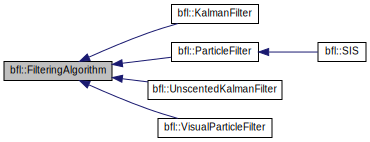
\includegraphics[width=350pt]{classbfl_1_1FilteringAlgorithm__inherit__graph}
\end{center}
\end{figure}
\subsection*{Public Member Functions}
\begin{DoxyCompactItemize}
\item 
virtual \mbox{\hyperlink{classbfl_1_1FilteringAlgorithm_ab286cc00b054717679fb13a3b709b1c4}{$\sim$\+Filtering\+Algorithm}} () noexcept
\item 
bool \mbox{\hyperlink{classbfl_1_1FilteringAlgorithm_a96651f8464190c0a56d79219a1017147}{boot}} ()
\item 
void \mbox{\hyperlink{classbfl_1_1FilteringAlgorithm_a009cbe5f4bbb16967f6c6ddcaed8fbb1}{run}} ()
\item 
bool \mbox{\hyperlink{classbfl_1_1FilteringAlgorithm_a40372c24fa050eb0274371172df0a244}{wait}} ()
\item 
void \mbox{\hyperlink{classbfl_1_1FilteringAlgorithm_a2403c62fbd7bd7f5cda56a84f5f30331}{reset}} ()
\item 
void \mbox{\hyperlink{classbfl_1_1FilteringAlgorithm_a6022859aa985474fb997343cc935b11e}{reboot}} ()
\item 
bool \mbox{\hyperlink{classbfl_1_1FilteringAlgorithm_a1dc912d89ee8f96d4f3e8209865c5308}{teardown}} ()
\item 
unsigned int \mbox{\hyperlink{classbfl_1_1FilteringAlgorithm_a8c43b1f3dac30934c0a03de348d4a29d}{get\+Filtering\+Step}} ()
\item 
bool \mbox{\hyperlink{classbfl_1_1FilteringAlgorithm_a5cfecab2c778620e2557237472bb1721}{is\+Running}} ()
\item 
virtual bool \mbox{\hyperlink{classbfl_1_1FilteringAlgorithm_ac8a718a614905d89d6a43bbbc70d68b2}{skip}} (const std\+::string \&what\+\_\+step, const bool status)=0
\end{DoxyCompactItemize}
\subsection*{Protected Member Functions}
\begin{DoxyCompactItemize}
\item 
virtual void \mbox{\hyperlink{classbfl_1_1FilteringAlgorithm_af2a072aa51407fe5544bdbb7ce466e2a}{initialization}} ()=0
\item 
virtual void \mbox{\hyperlink{classbfl_1_1FilteringAlgorithm_ab3bceb43b5810a4bf1da884b8a0b145a}{filtering\+Step}} ()=0
\item 
virtual void \mbox{\hyperlink{classbfl_1_1FilteringAlgorithm_acdfebf68405a427491e4dd9d020ae09b}{get\+Result}} ()=0
\item 
virtual bool \mbox{\hyperlink{classbfl_1_1FilteringAlgorithm_a5fc12882356f6906b102fbfff2bc4b7c}{run\+Condition}} ()=0
\end{DoxyCompactItemize}
\subsection*{Private Member Functions}
\begin{DoxyCompactItemize}
\item 
void \mbox{\hyperlink{classbfl_1_1FilteringAlgorithm_a139fe290f73939e72c88cb43c8ef7544}{filtering\+Recursion}} ()
\end{DoxyCompactItemize}
\subsection*{Private Attributes}
\begin{DoxyCompactItemize}
\item 
unsigned int \mbox{\hyperlink{classbfl_1_1FilteringAlgorithm_a1d08a5db263e415138d88c9a01535767}{filtering\+\_\+step\+\_\+}} = 0
\item 
std\+::thread \mbox{\hyperlink{classbfl_1_1FilteringAlgorithm_a2fa16711fd751628977afbbf9f7e9d6d}{filtering\+\_\+thread\+\_\+}}
\item 
std\+::mutex \mbox{\hyperlink{classbfl_1_1FilteringAlgorithm_a8983a40e915d3dbbc306d8f281ac449b}{mtx\+\_\+run\+\_\+}}
\item 
std\+::condition\+\_\+variable \mbox{\hyperlink{classbfl_1_1FilteringAlgorithm_ae92a6d82ce18c35516f42a7109c931af}{cv\+\_\+run\+\_\+}}
\item 
bool \mbox{\hyperlink{classbfl_1_1FilteringAlgorithm_a826eea2b551a2c2beab38394ed4c57c9}{run\+\_\+}} = false
\item 
bool \mbox{\hyperlink{classbfl_1_1FilteringAlgorithm_a4edf8ab29c4a1f8148ea276561299acb}{reset\+\_\+}} = false
\item 
bool \mbox{\hyperlink{classbfl_1_1FilteringAlgorithm_a3bc20cde7fc24767328f8a1ebd3e8cc8}{teardown\+\_\+}} = false
\end{DoxyCompactItemize}


\subsection{Detailed Description}


Definition at line 18 of file Filtering\+Algorithm.\+h.



\subsection{Constructor \& Destructor Documentation}
\mbox{\Hypertarget{classbfl_1_1FilteringAlgorithm_ab286cc00b054717679fb13a3b709b1c4}\label{classbfl_1_1FilteringAlgorithm_ab286cc00b054717679fb13a3b709b1c4}} 
\index{bfl\+::\+Filtering\+Algorithm@{bfl\+::\+Filtering\+Algorithm}!````~Filtering\+Algorithm@{$\sim$\+Filtering\+Algorithm}}
\index{````~Filtering\+Algorithm@{$\sim$\+Filtering\+Algorithm}!bfl\+::\+Filtering\+Algorithm@{bfl\+::\+Filtering\+Algorithm}}
\subsubsection{\texorpdfstring{$\sim$\+Filtering\+Algorithm()}{~FilteringAlgorithm()}}
{\footnotesize\ttfamily virtual bfl\+::\+Filtering\+Algorithm\+::$\sim$\+Filtering\+Algorithm (\begin{DoxyParamCaption}{ }\end{DoxyParamCaption})\hspace{0.3cm}{\ttfamily [inline]}, {\ttfamily [virtual]}, {\ttfamily [noexcept]}}



Definition at line 21 of file Filtering\+Algorithm.\+h.



\subsection{Member Function Documentation}
\mbox{\Hypertarget{classbfl_1_1FilteringAlgorithm_a96651f8464190c0a56d79219a1017147}\label{classbfl_1_1FilteringAlgorithm_a96651f8464190c0a56d79219a1017147}} 
\index{bfl\+::\+Filtering\+Algorithm@{bfl\+::\+Filtering\+Algorithm}!boot@{boot}}
\index{boot@{boot}!bfl\+::\+Filtering\+Algorithm@{bfl\+::\+Filtering\+Algorithm}}
\subsubsection{\texorpdfstring{boot()}{boot()}}
{\footnotesize\ttfamily bool Filtering\+Algorithm\+::boot (\begin{DoxyParamCaption}{ }\end{DoxyParamCaption})}



Definition at line 8 of file Filtering\+Algorithm.\+cpp.



References filtering\+\_\+thread\+\_\+, and filtering\+Recursion().

Here is the call graph for this function\+:
\nopagebreak
\begin{figure}[H]
\begin{center}
\leavevmode
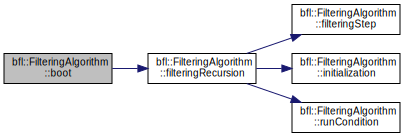
\includegraphics[width=350pt]{classbfl_1_1FilteringAlgorithm_a96651f8464190c0a56d79219a1017147_cgraph}
\end{center}
\end{figure}
\mbox{\Hypertarget{classbfl_1_1FilteringAlgorithm_a139fe290f73939e72c88cb43c8ef7544}\label{classbfl_1_1FilteringAlgorithm_a139fe290f73939e72c88cb43c8ef7544}} 
\index{bfl\+::\+Filtering\+Algorithm@{bfl\+::\+Filtering\+Algorithm}!filtering\+Recursion@{filtering\+Recursion}}
\index{filtering\+Recursion@{filtering\+Recursion}!bfl\+::\+Filtering\+Algorithm@{bfl\+::\+Filtering\+Algorithm}}
\subsubsection{\texorpdfstring{filtering\+Recursion()}{filteringRecursion()}}
{\footnotesize\ttfamily void Filtering\+Algorithm\+::filtering\+Recursion (\begin{DoxyParamCaption}{ }\end{DoxyParamCaption})\hspace{0.3cm}{\ttfamily [private]}}



Definition at line 98 of file Filtering\+Algorithm.\+cpp.



References cv\+\_\+run\+\_\+, filtering\+\_\+step\+\_\+, filtering\+Step(), initialization(), mtx\+\_\+run\+\_\+, reset\+\_\+, run\+\_\+, run\+Condition(), and teardown\+\_\+.



Referenced by boot().

Here is the call graph for this function\+:
\nopagebreak
\begin{figure}[H]
\begin{center}
\leavevmode
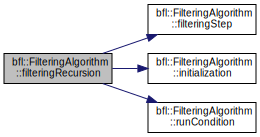
\includegraphics[width=332pt]{classbfl_1_1FilteringAlgorithm_a139fe290f73939e72c88cb43c8ef7544_cgraph}
\end{center}
\end{figure}
\mbox{\Hypertarget{classbfl_1_1FilteringAlgorithm_ab3bceb43b5810a4bf1da884b8a0b145a}\label{classbfl_1_1FilteringAlgorithm_ab3bceb43b5810a4bf1da884b8a0b145a}} 
\index{bfl\+::\+Filtering\+Algorithm@{bfl\+::\+Filtering\+Algorithm}!filtering\+Step@{filtering\+Step}}
\index{filtering\+Step@{filtering\+Step}!bfl\+::\+Filtering\+Algorithm@{bfl\+::\+Filtering\+Algorithm}}
\subsubsection{\texorpdfstring{filtering\+Step()}{filteringStep()}}
{\footnotesize\ttfamily virtual void bfl\+::\+Filtering\+Algorithm\+::filtering\+Step (\begin{DoxyParamCaption}{ }\end{DoxyParamCaption})\hspace{0.3cm}{\ttfamily [protected]}, {\ttfamily [pure virtual]}}



Implemented in \mbox{\hyperlink{classbfl_1_1SIS_a582f06cc5456d2cc6ed8f90087cbbb4c}{bfl\+::\+S\+IS}}, \mbox{\hyperlink{classbfl_1_1UnscentedKalmanFilter_a169451bb711a03ad2dc28a40e3ad867f}{bfl\+::\+Unscented\+Kalman\+Filter}}, and \mbox{\hyperlink{classbfl_1_1KalmanFilter_aac6bd54422cba06e34cb93cb8a659950}{bfl\+::\+Kalman\+Filter}}.



Referenced by filtering\+Recursion().

\mbox{\Hypertarget{classbfl_1_1FilteringAlgorithm_a8c43b1f3dac30934c0a03de348d4a29d}\label{classbfl_1_1FilteringAlgorithm_a8c43b1f3dac30934c0a03de348d4a29d}} 
\index{bfl\+::\+Filtering\+Algorithm@{bfl\+::\+Filtering\+Algorithm}!get\+Filtering\+Step@{get\+Filtering\+Step}}
\index{get\+Filtering\+Step@{get\+Filtering\+Step}!bfl\+::\+Filtering\+Algorithm@{bfl\+::\+Filtering\+Algorithm}}
\subsubsection{\texorpdfstring{get\+Filtering\+Step()}{getFilteringStep()}}
{\footnotesize\ttfamily unsigned int Filtering\+Algorithm\+::get\+Filtering\+Step (\begin{DoxyParamCaption}{ }\end{DoxyParamCaption})}



Definition at line 86 of file Filtering\+Algorithm.\+cpp.



References filtering\+\_\+step\+\_\+.

\mbox{\Hypertarget{classbfl_1_1FilteringAlgorithm_acdfebf68405a427491e4dd9d020ae09b}\label{classbfl_1_1FilteringAlgorithm_acdfebf68405a427491e4dd9d020ae09b}} 
\index{bfl\+::\+Filtering\+Algorithm@{bfl\+::\+Filtering\+Algorithm}!get\+Result@{get\+Result}}
\index{get\+Result@{get\+Result}!bfl\+::\+Filtering\+Algorithm@{bfl\+::\+Filtering\+Algorithm}}
\subsubsection{\texorpdfstring{get\+Result()}{getResult()}}
{\footnotesize\ttfamily virtual void bfl\+::\+Filtering\+Algorithm\+::get\+Result (\begin{DoxyParamCaption}{ }\end{DoxyParamCaption})\hspace{0.3cm}{\ttfamily [protected]}, {\ttfamily [pure virtual]}}



Implemented in \mbox{\hyperlink{classbfl_1_1SIS_a059da4c932379643ff7005fe4d0fda89}{bfl\+::\+S\+IS}}, \mbox{\hyperlink{classbfl_1_1UnscentedKalmanFilter_ad25c4f9143bbe834b3adfc81c78b6743}{bfl\+::\+Unscented\+Kalman\+Filter}}, and \mbox{\hyperlink{classbfl_1_1KalmanFilter_a24484fb845495f43628db19062937548}{bfl\+::\+Kalman\+Filter}}.

\mbox{\Hypertarget{classbfl_1_1FilteringAlgorithm_af2a072aa51407fe5544bdbb7ce466e2a}\label{classbfl_1_1FilteringAlgorithm_af2a072aa51407fe5544bdbb7ce466e2a}} 
\index{bfl\+::\+Filtering\+Algorithm@{bfl\+::\+Filtering\+Algorithm}!initialization@{initialization}}
\index{initialization@{initialization}!bfl\+::\+Filtering\+Algorithm@{bfl\+::\+Filtering\+Algorithm}}
\subsubsection{\texorpdfstring{initialization()}{initialization()}}
{\footnotesize\ttfamily virtual void bfl\+::\+Filtering\+Algorithm\+::initialization (\begin{DoxyParamCaption}{ }\end{DoxyParamCaption})\hspace{0.3cm}{\ttfamily [protected]}, {\ttfamily [pure virtual]}}



Implemented in \mbox{\hyperlink{classbfl_1_1SIS_aaf9f4a14d51804eddcd93aa8a5ccbba8}{bfl\+::\+S\+IS}}, \mbox{\hyperlink{classbfl_1_1UnscentedKalmanFilter_acd5cfc6344d9ce24fb980aa22ecf4895}{bfl\+::\+Unscented\+Kalman\+Filter}}, and \mbox{\hyperlink{classbfl_1_1KalmanFilter_a34482fcfad20be0559cea9c060c5f949}{bfl\+::\+Kalman\+Filter}}.



Referenced by filtering\+Recursion(), bfl\+::\+Visual\+Particle\+Filter\+::set\+Initialization(), and bfl\+::\+Particle\+Filter\+::set\+Initialization().

\mbox{\Hypertarget{classbfl_1_1FilteringAlgorithm_a5cfecab2c778620e2557237472bb1721}\label{classbfl_1_1FilteringAlgorithm_a5cfecab2c778620e2557237472bb1721}} 
\index{bfl\+::\+Filtering\+Algorithm@{bfl\+::\+Filtering\+Algorithm}!is\+Running@{is\+Running}}
\index{is\+Running@{is\+Running}!bfl\+::\+Filtering\+Algorithm@{bfl\+::\+Filtering\+Algorithm}}
\subsubsection{\texorpdfstring{is\+Running()}{isRunning()}}
{\footnotesize\ttfamily bool Filtering\+Algorithm\+::is\+Running (\begin{DoxyParamCaption}{ }\end{DoxyParamCaption})}



Definition at line 92 of file Filtering\+Algorithm.\+cpp.



References run\+\_\+.

\mbox{\Hypertarget{classbfl_1_1FilteringAlgorithm_a6022859aa985474fb997343cc935b11e}\label{classbfl_1_1FilteringAlgorithm_a6022859aa985474fb997343cc935b11e}} 
\index{bfl\+::\+Filtering\+Algorithm@{bfl\+::\+Filtering\+Algorithm}!reboot@{reboot}}
\index{reboot@{reboot}!bfl\+::\+Filtering\+Algorithm@{bfl\+::\+Filtering\+Algorithm}}
\subsubsection{\texorpdfstring{reboot()}{reboot()}}
{\footnotesize\ttfamily void Filtering\+Algorithm\+::reboot (\begin{DoxyParamCaption}{ }\end{DoxyParamCaption})}



Definition at line 66 of file Filtering\+Algorithm.\+cpp.



References cv\+\_\+run\+\_\+, mtx\+\_\+run\+\_\+, reset\+\_\+, and run\+\_\+.

\mbox{\Hypertarget{classbfl_1_1FilteringAlgorithm_a2403c62fbd7bd7f5cda56a84f5f30331}\label{classbfl_1_1FilteringAlgorithm_a2403c62fbd7bd7f5cda56a84f5f30331}} 
\index{bfl\+::\+Filtering\+Algorithm@{bfl\+::\+Filtering\+Algorithm}!reset@{reset}}
\index{reset@{reset}!bfl\+::\+Filtering\+Algorithm@{bfl\+::\+Filtering\+Algorithm}}
\subsubsection{\texorpdfstring{reset()}{reset()}}
{\footnotesize\ttfamily void Filtering\+Algorithm\+::reset (\begin{DoxyParamCaption}{ }\end{DoxyParamCaption})}



Definition at line 60 of file Filtering\+Algorithm.\+cpp.



References reset\+\_\+.

\mbox{\Hypertarget{classbfl_1_1FilteringAlgorithm_a009cbe5f4bbb16967f6c6ddcaed8fbb1}\label{classbfl_1_1FilteringAlgorithm_a009cbe5f4bbb16967f6c6ddcaed8fbb1}} 
\index{bfl\+::\+Filtering\+Algorithm@{bfl\+::\+Filtering\+Algorithm}!run@{run}}
\index{run@{run}!bfl\+::\+Filtering\+Algorithm@{bfl\+::\+Filtering\+Algorithm}}
\subsubsection{\texorpdfstring{run()}{run()}}
{\footnotesize\ttfamily void Filtering\+Algorithm\+::run (\begin{DoxyParamCaption}{ }\end{DoxyParamCaption})}



Definition at line 26 of file Filtering\+Algorithm.\+cpp.



References cv\+\_\+run\+\_\+, mtx\+\_\+run\+\_\+, and run\+\_\+.

\mbox{\Hypertarget{classbfl_1_1FilteringAlgorithm_a5fc12882356f6906b102fbfff2bc4b7c}\label{classbfl_1_1FilteringAlgorithm_a5fc12882356f6906b102fbfff2bc4b7c}} 
\index{bfl\+::\+Filtering\+Algorithm@{bfl\+::\+Filtering\+Algorithm}!run\+Condition@{run\+Condition}}
\index{run\+Condition@{run\+Condition}!bfl\+::\+Filtering\+Algorithm@{bfl\+::\+Filtering\+Algorithm}}
\subsubsection{\texorpdfstring{run\+Condition()}{runCondition()}}
{\footnotesize\ttfamily virtual bool bfl\+::\+Filtering\+Algorithm\+::run\+Condition (\begin{DoxyParamCaption}{ }\end{DoxyParamCaption})\hspace{0.3cm}{\ttfamily [protected]}, {\ttfamily [pure virtual]}}



Implemented in \mbox{\hyperlink{classbfl_1_1SIS_afb7cff1f7dae80e0e4ca84c925ca3ac3}{bfl\+::\+S\+IS}}.



Referenced by filtering\+Recursion().

\mbox{\Hypertarget{classbfl_1_1FilteringAlgorithm_ac8a718a614905d89d6a43bbbc70d68b2}\label{classbfl_1_1FilteringAlgorithm_ac8a718a614905d89d6a43bbbc70d68b2}} 
\index{bfl\+::\+Filtering\+Algorithm@{bfl\+::\+Filtering\+Algorithm}!skip@{skip}}
\index{skip@{skip}!bfl\+::\+Filtering\+Algorithm@{bfl\+::\+Filtering\+Algorithm}}
\subsubsection{\texorpdfstring{skip()}{skip()}}
{\footnotesize\ttfamily virtual bool bfl\+::\+Filtering\+Algorithm\+::skip (\begin{DoxyParamCaption}\item[{const std\+::string \&}]{what\+\_\+step,  }\item[{const bool}]{status }\end{DoxyParamCaption})\hspace{0.3cm}{\ttfamily [pure virtual]}}



Implemented in \mbox{\hyperlink{classbfl_1_1ParticleFilter_a2d7a5e7aaad179037273d35be229056d}{bfl\+::\+Particle\+Filter}}, and \mbox{\hyperlink{classbfl_1_1VisualParticleFilter_aab68e455c645bc1b7b8c3c2b476c2f9c}{bfl\+::\+Visual\+Particle\+Filter}}.

\mbox{\Hypertarget{classbfl_1_1FilteringAlgorithm_a1dc912d89ee8f96d4f3e8209865c5308}\label{classbfl_1_1FilteringAlgorithm_a1dc912d89ee8f96d4f3e8209865c5308}} 
\index{bfl\+::\+Filtering\+Algorithm@{bfl\+::\+Filtering\+Algorithm}!teardown@{teardown}}
\index{teardown@{teardown}!bfl\+::\+Filtering\+Algorithm@{bfl\+::\+Filtering\+Algorithm}}
\subsubsection{\texorpdfstring{teardown()}{teardown()}}
{\footnotesize\ttfamily bool Filtering\+Algorithm\+::teardown (\begin{DoxyParamCaption}{ }\end{DoxyParamCaption})}



Definition at line 75 of file Filtering\+Algorithm.\+cpp.



References teardown\+\_\+.

\mbox{\Hypertarget{classbfl_1_1FilteringAlgorithm_a40372c24fa050eb0274371172df0a244}\label{classbfl_1_1FilteringAlgorithm_a40372c24fa050eb0274371172df0a244}} 
\index{bfl\+::\+Filtering\+Algorithm@{bfl\+::\+Filtering\+Algorithm}!wait@{wait}}
\index{wait@{wait}!bfl\+::\+Filtering\+Algorithm@{bfl\+::\+Filtering\+Algorithm}}
\subsubsection{\texorpdfstring{wait()}{wait()}}
{\footnotesize\ttfamily bool Filtering\+Algorithm\+::wait (\begin{DoxyParamCaption}{ }\end{DoxyParamCaption})}



Definition at line 34 of file Filtering\+Algorithm.\+cpp.



References filtering\+\_\+thread\+\_\+.



\subsection{Member Data Documentation}
\mbox{\Hypertarget{classbfl_1_1FilteringAlgorithm_ae92a6d82ce18c35516f42a7109c931af}\label{classbfl_1_1FilteringAlgorithm_ae92a6d82ce18c35516f42a7109c931af}} 
\index{bfl\+::\+Filtering\+Algorithm@{bfl\+::\+Filtering\+Algorithm}!cv\+\_\+run\+\_\+@{cv\+\_\+run\+\_\+}}
\index{cv\+\_\+run\+\_\+@{cv\+\_\+run\+\_\+}!bfl\+::\+Filtering\+Algorithm@{bfl\+::\+Filtering\+Algorithm}}
\subsubsection{\texorpdfstring{cv\+\_\+run\+\_\+}{cv\_run\_}}
{\footnotesize\ttfamily std\+::condition\+\_\+variable bfl\+::\+Filtering\+Algorithm\+::cv\+\_\+run\+\_\+\hspace{0.3cm}{\ttfamily [private]}}



Definition at line 59 of file Filtering\+Algorithm.\+h.



Referenced by filtering\+Recursion(), reboot(), and run().

\mbox{\Hypertarget{classbfl_1_1FilteringAlgorithm_a1d08a5db263e415138d88c9a01535767}\label{classbfl_1_1FilteringAlgorithm_a1d08a5db263e415138d88c9a01535767}} 
\index{bfl\+::\+Filtering\+Algorithm@{bfl\+::\+Filtering\+Algorithm}!filtering\+\_\+step\+\_\+@{filtering\+\_\+step\+\_\+}}
\index{filtering\+\_\+step\+\_\+@{filtering\+\_\+step\+\_\+}!bfl\+::\+Filtering\+Algorithm@{bfl\+::\+Filtering\+Algorithm}}
\subsubsection{\texorpdfstring{filtering\+\_\+step\+\_\+}{filtering\_step\_}}
{\footnotesize\ttfamily unsigned int bfl\+::\+Filtering\+Algorithm\+::filtering\+\_\+step\+\_\+ = 0\hspace{0.3cm}{\ttfamily [private]}}



Definition at line 51 of file Filtering\+Algorithm.\+h.



Referenced by filtering\+Recursion(), and get\+Filtering\+Step().

\mbox{\Hypertarget{classbfl_1_1FilteringAlgorithm_a2fa16711fd751628977afbbf9f7e9d6d}\label{classbfl_1_1FilteringAlgorithm_a2fa16711fd751628977afbbf9f7e9d6d}} 
\index{bfl\+::\+Filtering\+Algorithm@{bfl\+::\+Filtering\+Algorithm}!filtering\+\_\+thread\+\_\+@{filtering\+\_\+thread\+\_\+}}
\index{filtering\+\_\+thread\+\_\+@{filtering\+\_\+thread\+\_\+}!bfl\+::\+Filtering\+Algorithm@{bfl\+::\+Filtering\+Algorithm}}
\subsubsection{\texorpdfstring{filtering\+\_\+thread\+\_\+}{filtering\_thread\_}}
{\footnotesize\ttfamily std\+::thread bfl\+::\+Filtering\+Algorithm\+::filtering\+\_\+thread\+\_\+\hspace{0.3cm}{\ttfamily [private]}}



Definition at line 53 of file Filtering\+Algorithm.\+h.



Referenced by boot(), and wait().

\mbox{\Hypertarget{classbfl_1_1FilteringAlgorithm_a8983a40e915d3dbbc306d8f281ac449b}\label{classbfl_1_1FilteringAlgorithm_a8983a40e915d3dbbc306d8f281ac449b}} 
\index{bfl\+::\+Filtering\+Algorithm@{bfl\+::\+Filtering\+Algorithm}!mtx\+\_\+run\+\_\+@{mtx\+\_\+run\+\_\+}}
\index{mtx\+\_\+run\+\_\+@{mtx\+\_\+run\+\_\+}!bfl\+::\+Filtering\+Algorithm@{bfl\+::\+Filtering\+Algorithm}}
\subsubsection{\texorpdfstring{mtx\+\_\+run\+\_\+}{mtx\_run\_}}
{\footnotesize\ttfamily std\+::mutex bfl\+::\+Filtering\+Algorithm\+::mtx\+\_\+run\+\_\+\hspace{0.3cm}{\ttfamily [private]}}



Definition at line 58 of file Filtering\+Algorithm.\+h.



Referenced by filtering\+Recursion(), reboot(), and run().

\mbox{\Hypertarget{classbfl_1_1FilteringAlgorithm_a4edf8ab29c4a1f8148ea276561299acb}\label{classbfl_1_1FilteringAlgorithm_a4edf8ab29c4a1f8148ea276561299acb}} 
\index{bfl\+::\+Filtering\+Algorithm@{bfl\+::\+Filtering\+Algorithm}!reset\+\_\+@{reset\+\_\+}}
\index{reset\+\_\+@{reset\+\_\+}!bfl\+::\+Filtering\+Algorithm@{bfl\+::\+Filtering\+Algorithm}}
\subsubsection{\texorpdfstring{reset\+\_\+}{reset\_}}
{\footnotesize\ttfamily bool bfl\+::\+Filtering\+Algorithm\+::reset\+\_\+ = false\hspace{0.3cm}{\ttfamily [private]}}



Definition at line 63 of file Filtering\+Algorithm.\+h.



Referenced by filtering\+Recursion(), reboot(), and reset().

\mbox{\Hypertarget{classbfl_1_1FilteringAlgorithm_a826eea2b551a2c2beab38394ed4c57c9}\label{classbfl_1_1FilteringAlgorithm_a826eea2b551a2c2beab38394ed4c57c9}} 
\index{bfl\+::\+Filtering\+Algorithm@{bfl\+::\+Filtering\+Algorithm}!run\+\_\+@{run\+\_\+}}
\index{run\+\_\+@{run\+\_\+}!bfl\+::\+Filtering\+Algorithm@{bfl\+::\+Filtering\+Algorithm}}
\subsubsection{\texorpdfstring{run\+\_\+}{run\_}}
{\footnotesize\ttfamily bool bfl\+::\+Filtering\+Algorithm\+::run\+\_\+ = false\hspace{0.3cm}{\ttfamily [private]}}



Definition at line 61 of file Filtering\+Algorithm.\+h.



Referenced by filtering\+Recursion(), is\+Running(), reboot(), and run().

\mbox{\Hypertarget{classbfl_1_1FilteringAlgorithm_a3bc20cde7fc24767328f8a1ebd3e8cc8}\label{classbfl_1_1FilteringAlgorithm_a3bc20cde7fc24767328f8a1ebd3e8cc8}} 
\index{bfl\+::\+Filtering\+Algorithm@{bfl\+::\+Filtering\+Algorithm}!teardown\+\_\+@{teardown\+\_\+}}
\index{teardown\+\_\+@{teardown\+\_\+}!bfl\+::\+Filtering\+Algorithm@{bfl\+::\+Filtering\+Algorithm}}
\subsubsection{\texorpdfstring{teardown\+\_\+}{teardown\_}}
{\footnotesize\ttfamily bool bfl\+::\+Filtering\+Algorithm\+::teardown\+\_\+ = false\hspace{0.3cm}{\ttfamily [private]}}



Definition at line 65 of file Filtering\+Algorithm.\+h.



Referenced by filtering\+Recursion(), and teardown().



The documentation for this class was generated from the following files\+:\begin{DoxyCompactItemize}
\item 
C\+:/\+Users/cfantacci/\+Git\+Hub/bayes-\/filters-\/lib/src/\+Bayes\+Filters/include/\+Bayes\+Filters/\mbox{\hyperlink{FilteringAlgorithm_8h}{Filtering\+Algorithm.\+h}}\item 
C\+:/\+Users/cfantacci/\+Git\+Hub/bayes-\/filters-\/lib/src/\+Bayes\+Filters/src/\mbox{\hyperlink{FilteringAlgorithm_8cpp}{Filtering\+Algorithm.\+cpp}}\end{DoxyCompactItemize}

\input{classbfl_1_1FilteringContext}
\input{classbfl_1_1HistoryBuffer}
\hypertarget{classbfl_1_1Initialization}{}\section{bfl\+:\+:Initialization Class Reference}
\label{classbfl_1_1Initialization}\index{bfl\+::\+Initialization@{bfl\+::\+Initialization}}


{\ttfamily \#include $<$Initialization.\+h$>$}

\subsection*{Public Member Functions}
\begin{DoxyCompactItemize}
\item 
virtual \mbox{\hyperlink{classbfl_1_1Initialization_a5ee48ad764e9deebe023964b9be32e33}{$\sim$\+Initialization}} () noexcept
\item 
virtual void \mbox{\hyperlink{classbfl_1_1Initialization_aabd4858e78115b904de19d7282f0aad7}{initialize}} (Eigen\+::\+Ref$<$ Eigen\+::\+Matrix\+Xf $>$ states, Eigen\+::\+Ref$<$ Eigen\+::\+Vector\+Xf $>$ weights)=0
\end{DoxyCompactItemize}


\subsection{Detailed Description}


Definition at line 11 of file Initialization.\+h.



\subsection{Constructor \& Destructor Documentation}
\mbox{\Hypertarget{classbfl_1_1Initialization_a5ee48ad764e9deebe023964b9be32e33}\label{classbfl_1_1Initialization_a5ee48ad764e9deebe023964b9be32e33}} 
\index{bfl\+::\+Initialization@{bfl\+::\+Initialization}!````~Initialization@{$\sim$\+Initialization}}
\index{````~Initialization@{$\sim$\+Initialization}!bfl\+::\+Initialization@{bfl\+::\+Initialization}}
\subsubsection{\texorpdfstring{$\sim$\+Initialization()}{~Initialization()}}
{\footnotesize\ttfamily virtual bfl\+::\+Initialization\+::$\sim$\+Initialization (\begin{DoxyParamCaption}{ }\end{DoxyParamCaption})\hspace{0.3cm}{\ttfamily [inline]}, {\ttfamily [virtual]}, {\ttfamily [noexcept]}}



Definition at line 14 of file Initialization.\+h.



\subsection{Member Function Documentation}
\mbox{\Hypertarget{classbfl_1_1Initialization_aabd4858e78115b904de19d7282f0aad7}\label{classbfl_1_1Initialization_aabd4858e78115b904de19d7282f0aad7}} 
\index{bfl\+::\+Initialization@{bfl\+::\+Initialization}!initialize@{initialize}}
\index{initialize@{initialize}!bfl\+::\+Initialization@{bfl\+::\+Initialization}}
\subsubsection{\texorpdfstring{initialize()}{initialize()}}
{\footnotesize\ttfamily virtual void bfl\+::\+Initialization\+::initialize (\begin{DoxyParamCaption}\item[{Eigen\+::\+Ref$<$ Eigen\+::\+Matrix\+Xf $>$}]{states,  }\item[{Eigen\+::\+Ref$<$ Eigen\+::\+Vector\+Xf $>$}]{weights }\end{DoxyParamCaption})\hspace{0.3cm}{\ttfamily [pure virtual]}}



The documentation for this class was generated from the following file\+:\begin{DoxyCompactItemize}
\item 
C\+:/\+Users/cfantacci/\+Git\+Hub/bayes-\/filters-\/lib/src/\+Bayes\+Filters/include/\+Bayes\+Filters/\mbox{\hyperlink{Initialization_8h}{Initialization.\+h}}\end{DoxyCompactItemize}

\hypertarget{classbfl_1_1KalmanFilter}{}\section{bfl\+:\+:Kalman\+Filter Class Reference}
\label{classbfl_1_1KalmanFilter}\index{bfl\+::\+Kalman\+Filter@{bfl\+::\+Kalman\+Filter}}


{\ttfamily \#include $<$Kalman\+Filter.\+h$>$}



Inheritance diagram for bfl\+:\+:Kalman\+Filter\+:
\nopagebreak
\begin{figure}[H]
\begin{center}
\leavevmode
\includegraphics[width=188pt]{classbfl_1_1KalmanFilter__inherit__graph}
\end{center}
\end{figure}
\subsection*{Public Member Functions}
\begin{DoxyCompactItemize}
\item 
\mbox{\hyperlink{classbfl_1_1KalmanFilter_aab2cc3677e9fcb19fff16b84c997f30a}{Kalman\+Filter}} ()
\item 
virtual \mbox{\hyperlink{classbfl_1_1KalmanFilter_ae400948b72785980cef6fe0794e481fe}{$\sim$\+Kalman\+Filter}} () noexcept
\item 
void \mbox{\hyperlink{classbfl_1_1KalmanFilter_a34482fcfad20be0559cea9c060c5f949}{initialization}} () override
\item 
void \mbox{\hyperlink{classbfl_1_1KalmanFilter_aac6bd54422cba06e34cb93cb8a659950}{filtering\+Step}} () override
\item 
void \mbox{\hyperlink{classbfl_1_1KalmanFilter_a24484fb845495f43628db19062937548}{get\+Result}} () override
\item 
bool \mbox{\hyperlink{classbfl_1_1FilteringAlgorithm_a96651f8464190c0a56d79219a1017147}{boot}} ()
\item 
void \mbox{\hyperlink{classbfl_1_1FilteringAlgorithm_a009cbe5f4bbb16967f6c6ddcaed8fbb1}{run}} ()
\item 
bool \mbox{\hyperlink{classbfl_1_1FilteringAlgorithm_a40372c24fa050eb0274371172df0a244}{wait}} ()
\item 
void \mbox{\hyperlink{classbfl_1_1FilteringAlgorithm_a2403c62fbd7bd7f5cda56a84f5f30331}{reset}} ()
\item 
void \mbox{\hyperlink{classbfl_1_1FilteringAlgorithm_a6022859aa985474fb997343cc935b11e}{reboot}} ()
\item 
bool \mbox{\hyperlink{classbfl_1_1FilteringAlgorithm_a1dc912d89ee8f96d4f3e8209865c5308}{teardown}} ()
\item 
unsigned int \mbox{\hyperlink{classbfl_1_1FilteringAlgorithm_a8c43b1f3dac30934c0a03de348d4a29d}{get\+Filtering\+Step}} ()
\item 
bool \mbox{\hyperlink{classbfl_1_1FilteringAlgorithm_a5cfecab2c778620e2557237472bb1721}{is\+Running}} ()
\item 
virtual bool \mbox{\hyperlink{classbfl_1_1FilteringAlgorithm_ac8a718a614905d89d6a43bbbc70d68b2}{skip}} (const std\+::string \&what\+\_\+step, const bool status)=0
\end{DoxyCompactItemize}
\subsection*{Protected Member Functions}
\begin{DoxyCompactItemize}
\item 
virtual bool \mbox{\hyperlink{classbfl_1_1FilteringAlgorithm_a5fc12882356f6906b102fbfff2bc4b7c}{run\+Condition}} ()=0
\end{DoxyCompactItemize}


\subsection{Detailed Description}


Definition at line 11 of file Kalman\+Filter.\+h.



\subsection{Constructor \& Destructor Documentation}
\mbox{\Hypertarget{classbfl_1_1KalmanFilter_aab2cc3677e9fcb19fff16b84c997f30a}\label{classbfl_1_1KalmanFilter_aab2cc3677e9fcb19fff16b84c997f30a}} 
\index{bfl\+::\+Kalman\+Filter@{bfl\+::\+Kalman\+Filter}!Kalman\+Filter@{Kalman\+Filter}}
\index{Kalman\+Filter@{Kalman\+Filter}!bfl\+::\+Kalman\+Filter@{bfl\+::\+Kalman\+Filter}}
\subsubsection{\texorpdfstring{Kalman\+Filter()}{KalmanFilter()}}
{\footnotesize\ttfamily Kalman\+Filter\+::\+Kalman\+Filter (\begin{DoxyParamCaption}{ }\end{DoxyParamCaption})}



Definition at line 6 of file Kalman\+Filter.\+cpp.

\mbox{\Hypertarget{classbfl_1_1KalmanFilter_ae400948b72785980cef6fe0794e481fe}\label{classbfl_1_1KalmanFilter_ae400948b72785980cef6fe0794e481fe}} 
\index{bfl\+::\+Kalman\+Filter@{bfl\+::\+Kalman\+Filter}!````~Kalman\+Filter@{$\sim$\+Kalman\+Filter}}
\index{````~Kalman\+Filter@{$\sim$\+Kalman\+Filter}!bfl\+::\+Kalman\+Filter@{bfl\+::\+Kalman\+Filter}}
\subsubsection{\texorpdfstring{$\sim$\+Kalman\+Filter()}{~KalmanFilter()}}
{\footnotesize\ttfamily Kalman\+Filter\+::$\sim$\+Kalman\+Filter (\begin{DoxyParamCaption}{ }\end{DoxyParamCaption})\hspace{0.3cm}{\ttfamily [virtual]}, {\ttfamily [noexcept]}}



Definition at line 9 of file Kalman\+Filter.\+cpp.



\subsection{Member Function Documentation}
\mbox{\Hypertarget{classbfl_1_1FilteringAlgorithm_a96651f8464190c0a56d79219a1017147}\label{classbfl_1_1FilteringAlgorithm_a96651f8464190c0a56d79219a1017147}} 
\index{bfl\+::\+Kalman\+Filter@{bfl\+::\+Kalman\+Filter}!boot@{boot}}
\index{boot@{boot}!bfl\+::\+Kalman\+Filter@{bfl\+::\+Kalman\+Filter}}
\subsubsection{\texorpdfstring{boot()}{boot()}}
{\footnotesize\ttfamily bool Filtering\+Algorithm\+::boot (\begin{DoxyParamCaption}{ }\end{DoxyParamCaption})\hspace{0.3cm}{\ttfamily [inherited]}}



Definition at line 8 of file Filtering\+Algorithm.\+cpp.



References bfl\+::\+Filtering\+Algorithm\+::filtering\+\_\+thread\+\_\+, and bfl\+::\+Filtering\+Algorithm\+::filtering\+Recursion().

Here is the call graph for this function\+:
\nopagebreak
\begin{figure}[H]
\begin{center}
\leavevmode
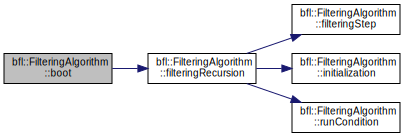
\includegraphics[width=350pt]{classbfl_1_1FilteringAlgorithm_a96651f8464190c0a56d79219a1017147_cgraph}
\end{center}
\end{figure}
\mbox{\Hypertarget{classbfl_1_1KalmanFilter_aac6bd54422cba06e34cb93cb8a659950}\label{classbfl_1_1KalmanFilter_aac6bd54422cba06e34cb93cb8a659950}} 
\index{bfl\+::\+Kalman\+Filter@{bfl\+::\+Kalman\+Filter}!filtering\+Step@{filtering\+Step}}
\index{filtering\+Step@{filtering\+Step}!bfl\+::\+Kalman\+Filter@{bfl\+::\+Kalman\+Filter}}
\subsubsection{\texorpdfstring{filtering\+Step()}{filteringStep()}}
{\footnotesize\ttfamily void Kalman\+Filter\+::filtering\+Step (\begin{DoxyParamCaption}{ }\end{DoxyParamCaption})\hspace{0.3cm}{\ttfamily [override]}, {\ttfamily [virtual]}}



Implements \mbox{\hyperlink{classbfl_1_1FilteringAlgorithm_ab3bceb43b5810a4bf1da884b8a0b145a}{bfl\+::\+Filtering\+Algorithm}}.



Definition at line 15 of file Kalman\+Filter.\+cpp.

\mbox{\Hypertarget{classbfl_1_1FilteringAlgorithm_a8c43b1f3dac30934c0a03de348d4a29d}\label{classbfl_1_1FilteringAlgorithm_a8c43b1f3dac30934c0a03de348d4a29d}} 
\index{bfl\+::\+Kalman\+Filter@{bfl\+::\+Kalman\+Filter}!get\+Filtering\+Step@{get\+Filtering\+Step}}
\index{get\+Filtering\+Step@{get\+Filtering\+Step}!bfl\+::\+Kalman\+Filter@{bfl\+::\+Kalman\+Filter}}
\subsubsection{\texorpdfstring{get\+Filtering\+Step()}{getFilteringStep()}}
{\footnotesize\ttfamily unsigned int Filtering\+Algorithm\+::get\+Filtering\+Step (\begin{DoxyParamCaption}{ }\end{DoxyParamCaption})\hspace{0.3cm}{\ttfamily [inherited]}}



Definition at line 86 of file Filtering\+Algorithm.\+cpp.



References bfl\+::\+Filtering\+Algorithm\+::filtering\+\_\+step\+\_\+.

\mbox{\Hypertarget{classbfl_1_1KalmanFilter_a24484fb845495f43628db19062937548}\label{classbfl_1_1KalmanFilter_a24484fb845495f43628db19062937548}} 
\index{bfl\+::\+Kalman\+Filter@{bfl\+::\+Kalman\+Filter}!get\+Result@{get\+Result}}
\index{get\+Result@{get\+Result}!bfl\+::\+Kalman\+Filter@{bfl\+::\+Kalman\+Filter}}
\subsubsection{\texorpdfstring{get\+Result()}{getResult()}}
{\footnotesize\ttfamily void Kalman\+Filter\+::get\+Result (\begin{DoxyParamCaption}{ }\end{DoxyParamCaption})\hspace{0.3cm}{\ttfamily [override]}, {\ttfamily [virtual]}}



Implements \mbox{\hyperlink{classbfl_1_1FilteringAlgorithm_acdfebf68405a427491e4dd9d020ae09b}{bfl\+::\+Filtering\+Algorithm}}.



Definition at line 18 of file Kalman\+Filter.\+cpp.

\mbox{\Hypertarget{classbfl_1_1KalmanFilter_a34482fcfad20be0559cea9c060c5f949}\label{classbfl_1_1KalmanFilter_a34482fcfad20be0559cea9c060c5f949}} 
\index{bfl\+::\+Kalman\+Filter@{bfl\+::\+Kalman\+Filter}!initialization@{initialization}}
\index{initialization@{initialization}!bfl\+::\+Kalman\+Filter@{bfl\+::\+Kalman\+Filter}}
\subsubsection{\texorpdfstring{initialization()}{initialization()}}
{\footnotesize\ttfamily void Kalman\+Filter\+::initialization (\begin{DoxyParamCaption}{ }\end{DoxyParamCaption})\hspace{0.3cm}{\ttfamily [override]}, {\ttfamily [virtual]}}



Implements \mbox{\hyperlink{classbfl_1_1FilteringAlgorithm_af2a072aa51407fe5544bdbb7ce466e2a}{bfl\+::\+Filtering\+Algorithm}}.



Definition at line 12 of file Kalman\+Filter.\+cpp.

\mbox{\Hypertarget{classbfl_1_1FilteringAlgorithm_a5cfecab2c778620e2557237472bb1721}\label{classbfl_1_1FilteringAlgorithm_a5cfecab2c778620e2557237472bb1721}} 
\index{bfl\+::\+Kalman\+Filter@{bfl\+::\+Kalman\+Filter}!is\+Running@{is\+Running}}
\index{is\+Running@{is\+Running}!bfl\+::\+Kalman\+Filter@{bfl\+::\+Kalman\+Filter}}
\subsubsection{\texorpdfstring{is\+Running()}{isRunning()}}
{\footnotesize\ttfamily bool Filtering\+Algorithm\+::is\+Running (\begin{DoxyParamCaption}{ }\end{DoxyParamCaption})\hspace{0.3cm}{\ttfamily [inherited]}}



Definition at line 92 of file Filtering\+Algorithm.\+cpp.



References bfl\+::\+Filtering\+Algorithm\+::run\+\_\+.

\mbox{\Hypertarget{classbfl_1_1FilteringAlgorithm_a6022859aa985474fb997343cc935b11e}\label{classbfl_1_1FilteringAlgorithm_a6022859aa985474fb997343cc935b11e}} 
\index{bfl\+::\+Kalman\+Filter@{bfl\+::\+Kalman\+Filter}!reboot@{reboot}}
\index{reboot@{reboot}!bfl\+::\+Kalman\+Filter@{bfl\+::\+Kalman\+Filter}}
\subsubsection{\texorpdfstring{reboot()}{reboot()}}
{\footnotesize\ttfamily void Filtering\+Algorithm\+::reboot (\begin{DoxyParamCaption}{ }\end{DoxyParamCaption})\hspace{0.3cm}{\ttfamily [inherited]}}



Definition at line 66 of file Filtering\+Algorithm.\+cpp.



References bfl\+::\+Filtering\+Algorithm\+::cv\+\_\+run\+\_\+, bfl\+::\+Filtering\+Algorithm\+::mtx\+\_\+run\+\_\+, bfl\+::\+Filtering\+Algorithm\+::reset\+\_\+, and bfl\+::\+Filtering\+Algorithm\+::run\+\_\+.

\mbox{\Hypertarget{classbfl_1_1FilteringAlgorithm_a2403c62fbd7bd7f5cda56a84f5f30331}\label{classbfl_1_1FilteringAlgorithm_a2403c62fbd7bd7f5cda56a84f5f30331}} 
\index{bfl\+::\+Kalman\+Filter@{bfl\+::\+Kalman\+Filter}!reset@{reset}}
\index{reset@{reset}!bfl\+::\+Kalman\+Filter@{bfl\+::\+Kalman\+Filter}}
\subsubsection{\texorpdfstring{reset()}{reset()}}
{\footnotesize\ttfamily void Filtering\+Algorithm\+::reset (\begin{DoxyParamCaption}{ }\end{DoxyParamCaption})\hspace{0.3cm}{\ttfamily [inherited]}}



Definition at line 60 of file Filtering\+Algorithm.\+cpp.



References bfl\+::\+Filtering\+Algorithm\+::reset\+\_\+.

\mbox{\Hypertarget{classbfl_1_1FilteringAlgorithm_a009cbe5f4bbb16967f6c6ddcaed8fbb1}\label{classbfl_1_1FilteringAlgorithm_a009cbe5f4bbb16967f6c6ddcaed8fbb1}} 
\index{bfl\+::\+Kalman\+Filter@{bfl\+::\+Kalman\+Filter}!run@{run}}
\index{run@{run}!bfl\+::\+Kalman\+Filter@{bfl\+::\+Kalman\+Filter}}
\subsubsection{\texorpdfstring{run()}{run()}}
{\footnotesize\ttfamily void Filtering\+Algorithm\+::run (\begin{DoxyParamCaption}{ }\end{DoxyParamCaption})\hspace{0.3cm}{\ttfamily [inherited]}}



Definition at line 26 of file Filtering\+Algorithm.\+cpp.



References bfl\+::\+Filtering\+Algorithm\+::cv\+\_\+run\+\_\+, bfl\+::\+Filtering\+Algorithm\+::mtx\+\_\+run\+\_\+, and bfl\+::\+Filtering\+Algorithm\+::run\+\_\+.

\mbox{\Hypertarget{classbfl_1_1FilteringAlgorithm_a5fc12882356f6906b102fbfff2bc4b7c}\label{classbfl_1_1FilteringAlgorithm_a5fc12882356f6906b102fbfff2bc4b7c}} 
\index{bfl\+::\+Kalman\+Filter@{bfl\+::\+Kalman\+Filter}!run\+Condition@{run\+Condition}}
\index{run\+Condition@{run\+Condition}!bfl\+::\+Kalman\+Filter@{bfl\+::\+Kalman\+Filter}}
\subsubsection{\texorpdfstring{run\+Condition()}{runCondition()}}
{\footnotesize\ttfamily virtual bool bfl\+::\+Filtering\+Algorithm\+::run\+Condition (\begin{DoxyParamCaption}{ }\end{DoxyParamCaption})\hspace{0.3cm}{\ttfamily [protected]}, {\ttfamily [pure virtual]}, {\ttfamily [inherited]}}



Implemented in \mbox{\hyperlink{classbfl_1_1SIS_afb7cff1f7dae80e0e4ca84c925ca3ac3}{bfl\+::\+S\+IS}}.



Referenced by bfl\+::\+Filtering\+Algorithm\+::filtering\+Recursion().

\mbox{\Hypertarget{classbfl_1_1FilteringAlgorithm_ac8a718a614905d89d6a43bbbc70d68b2}\label{classbfl_1_1FilteringAlgorithm_ac8a718a614905d89d6a43bbbc70d68b2}} 
\index{bfl\+::\+Kalman\+Filter@{bfl\+::\+Kalman\+Filter}!skip@{skip}}
\index{skip@{skip}!bfl\+::\+Kalman\+Filter@{bfl\+::\+Kalman\+Filter}}
\subsubsection{\texorpdfstring{skip()}{skip()}}
{\footnotesize\ttfamily virtual bool bfl\+::\+Filtering\+Algorithm\+::skip (\begin{DoxyParamCaption}\item[{const std\+::string \&}]{what\+\_\+step,  }\item[{const bool}]{status }\end{DoxyParamCaption})\hspace{0.3cm}{\ttfamily [pure virtual]}, {\ttfamily [inherited]}}



Implemented in \mbox{\hyperlink{classbfl_1_1ParticleFilter_a2d7a5e7aaad179037273d35be229056d}{bfl\+::\+Particle\+Filter}}, and \mbox{\hyperlink{classbfl_1_1VisualParticleFilter_aab68e455c645bc1b7b8c3c2b476c2f9c}{bfl\+::\+Visual\+Particle\+Filter}}.

\mbox{\Hypertarget{classbfl_1_1FilteringAlgorithm_a1dc912d89ee8f96d4f3e8209865c5308}\label{classbfl_1_1FilteringAlgorithm_a1dc912d89ee8f96d4f3e8209865c5308}} 
\index{bfl\+::\+Kalman\+Filter@{bfl\+::\+Kalman\+Filter}!teardown@{teardown}}
\index{teardown@{teardown}!bfl\+::\+Kalman\+Filter@{bfl\+::\+Kalman\+Filter}}
\subsubsection{\texorpdfstring{teardown()}{teardown()}}
{\footnotesize\ttfamily bool Filtering\+Algorithm\+::teardown (\begin{DoxyParamCaption}{ }\end{DoxyParamCaption})\hspace{0.3cm}{\ttfamily [inherited]}}



Definition at line 75 of file Filtering\+Algorithm.\+cpp.



References bfl\+::\+Filtering\+Algorithm\+::teardown\+\_\+.

\mbox{\Hypertarget{classbfl_1_1FilteringAlgorithm_a40372c24fa050eb0274371172df0a244}\label{classbfl_1_1FilteringAlgorithm_a40372c24fa050eb0274371172df0a244}} 
\index{bfl\+::\+Kalman\+Filter@{bfl\+::\+Kalman\+Filter}!wait@{wait}}
\index{wait@{wait}!bfl\+::\+Kalman\+Filter@{bfl\+::\+Kalman\+Filter}}
\subsubsection{\texorpdfstring{wait()}{wait()}}
{\footnotesize\ttfamily bool Filtering\+Algorithm\+::wait (\begin{DoxyParamCaption}{ }\end{DoxyParamCaption})\hspace{0.3cm}{\ttfamily [inherited]}}



Definition at line 34 of file Filtering\+Algorithm.\+cpp.



References bfl\+::\+Filtering\+Algorithm\+::filtering\+\_\+thread\+\_\+.



The documentation for this class was generated from the following files\+:\begin{DoxyCompactItemize}
\item 
C\+:/\+Users/cfantacci/\+Git\+Hub/bayes-\/filters-\/lib/src/\+Bayes\+Filters/include/\+Bayes\+Filters/\mbox{\hyperlink{KalmanFilter_8h}{Kalman\+Filter.\+h}}\item 
C\+:/\+Users/cfantacci/\+Git\+Hub/bayes-\/filters-\/lib/src/\+Bayes\+Filters/src/\mbox{\hyperlink{KalmanFilter_8cpp}{Kalman\+Filter.\+cpp}}\end{DoxyCompactItemize}

\hypertarget{classbfl_1_1LinearSensor}{}\section{bfl\+:\+:Linear\+Sensor Class Reference}
\label{classbfl_1_1LinearSensor}\index{bfl\+::\+Linear\+Sensor@{bfl\+::\+Linear\+Sensor}}


{\ttfamily \#include $<$Linear\+Sensor.\+h$>$}



Inheritance diagram for bfl\+:\+:Linear\+Sensor\+:
\nopagebreak
\begin{figure}[H]
\begin{center}
\leavevmode
\includegraphics[width=190pt]{classbfl_1_1LinearSensor__inherit__graph}
\end{center}
\end{figure}
\subsection*{Public Member Functions}
\begin{DoxyCompactItemize}
\item 
\mbox{\hyperlink{classbfl_1_1LinearSensor_a854aed4f95acda27e216c4a2415b55bf}{Linear\+Sensor}} (float sigma\+\_\+x, float sigma\+\_\+y, unsigned int seed) noexcept
\item 
\mbox{\hyperlink{classbfl_1_1LinearSensor_abbd0d6d3a0deb476e1bacaf646dac55f}{Linear\+Sensor}} (float sigma\+\_\+x, float sigma\+\_\+y) noexcept
\item 
\mbox{\hyperlink{classbfl_1_1LinearSensor_a97d9226a08646f7c97a0e1b0cc0cb672}{Linear\+Sensor}} () noexcept
\item 
\mbox{\hyperlink{classbfl_1_1LinearSensor_a18250e7dc68c624b40c6d5312ef516a1}{Linear\+Sensor}} (const \mbox{\hyperlink{classbfl_1_1LinearSensor}{Linear\+Sensor}} \&lin\+\_\+sense)
\item 
\mbox{\hyperlink{classbfl_1_1LinearSensor_a670ab864282594958582114039c11484}{Linear\+Sensor}} (\mbox{\hyperlink{classbfl_1_1LinearSensor}{Linear\+Sensor}} \&\&lin\+\_\+sense) noexcept
\item 
virtual \mbox{\hyperlink{classbfl_1_1LinearSensor_a667f4b3eb18dd9a45b60288aa4f57939}{$\sim$\+Linear\+Sensor}} () noexcept
\item 
\mbox{\hyperlink{classbfl_1_1LinearSensor}{Linear\+Sensor}} \& \mbox{\hyperlink{classbfl_1_1LinearSensor_a83054bf80986f7b1772e71fdb8b37040}{operator=}} (const \mbox{\hyperlink{classbfl_1_1LinearSensor}{Linear\+Sensor}} \&lin\+\_\+sense) noexcept
\item 
\mbox{\hyperlink{classbfl_1_1LinearSensor}{Linear\+Sensor}} \& \mbox{\hyperlink{classbfl_1_1LinearSensor_aa93327ef56a19a9712f736d12fbf2651}{operator=}} (\mbox{\hyperlink{classbfl_1_1LinearSensor}{Linear\+Sensor}} \&\&lin\+\_\+sense) noexcept
\item 
void \mbox{\hyperlink{classbfl_1_1LinearSensor_ae53acb6051164c0bcd32d5a6f88e5962}{observe}} (const Eigen\+::\+Ref$<$ const Eigen\+::\+Matrix\+Xf $>$ \&cur\+\_\+states, Eigen\+::\+Ref$<$ Eigen\+::\+Matrix\+Xf $>$ observations) override
\item 
void \mbox{\hyperlink{classbfl_1_1LinearSensor_a36f36ae6b935a8c535b553ff6a265f6a}{measure}} (const Eigen\+::\+Ref$<$ const Eigen\+::\+Matrix\+Xf $>$ \&cur\+\_\+states, Eigen\+::\+Ref$<$ Eigen\+::\+Matrix\+Xf $>$ measurements) override
\item 
Eigen\+::\+Matrix\+Xf \mbox{\hyperlink{classbfl_1_1LinearSensor_a5079f70d2a2995cff4ad3210dd1795f7}{get\+Noise\+Sample}} (const int num) override
\item 
Eigen\+::\+Matrix\+Xf \mbox{\hyperlink{classbfl_1_1LinearSensor_a7773e8de7eb58b07b1ca781b20d8537e}{get\+Noise\+Covariance\+Matrix}} () override
\item 
bool \mbox{\hyperlink{classbfl_1_1LinearSensor_a3d20baf95d4ea62c536c87e68238852f}{set\+Property}} (const std\+::string property) override
\end{DoxyCompactItemize}
\subsection*{Protected Attributes}
\begin{DoxyCompactItemize}
\item 
float \mbox{\hyperlink{classbfl_1_1LinearSensor_a3d9edc1da64faf44c02e6fb3b869bf3b}{sigma\+\_\+x\+\_\+}}
\item 
float \mbox{\hyperlink{classbfl_1_1LinearSensor_a6b017eefd02cd452f740af7ece2f0374}{sigma\+\_\+y\+\_\+}}
\item 
Eigen\+::\+Matrix\+Xf \mbox{\hyperlink{classbfl_1_1LinearSensor_ae6df14a628525b334062c104e85df7ff}{H\+\_\+}}
\item 
Eigen\+::\+Matrix2f \mbox{\hyperlink{classbfl_1_1LinearSensor_a3c8550ed25965c8e946a77602e44d87b}{R\+\_\+}}
\item 
Eigen\+::\+Matrix2f \mbox{\hyperlink{classbfl_1_1LinearSensor_ac061b358b032a56844a48cb2024fe694}{sqrt\+\_\+\+R\+\_\+}}
\item 
std\+::mt19937\+\_\+64 \mbox{\hyperlink{classbfl_1_1LinearSensor_a564abeae2ab7fb98886f0a7952181a75}{generator\+\_\+}}
\item 
std\+::normal\+\_\+distribution$<$ float $>$ \mbox{\hyperlink{classbfl_1_1LinearSensor_a5ef72350f0591e2f95d80cf5818a5366}{distribution\+\_\+}}
\item 
std\+::function$<$ float()$>$ \mbox{\hyperlink{classbfl_1_1LinearSensor_a9c3d6ac31fc2aeade2d47cf0c9677cb1}{gauss\+\_\+rnd\+\_\+sample\+\_\+}}
\end{DoxyCompactItemize}


\subsection{Detailed Description}


Definition at line 14 of file Linear\+Sensor.\+h.



\subsection{Constructor \& Destructor Documentation}
\mbox{\Hypertarget{classbfl_1_1LinearSensor_a854aed4f95acda27e216c4a2415b55bf}\label{classbfl_1_1LinearSensor_a854aed4f95acda27e216c4a2415b55bf}} 
\index{bfl\+::\+Linear\+Sensor@{bfl\+::\+Linear\+Sensor}!Linear\+Sensor@{Linear\+Sensor}}
\index{Linear\+Sensor@{Linear\+Sensor}!bfl\+::\+Linear\+Sensor@{bfl\+::\+Linear\+Sensor}}
\subsubsection{\texorpdfstring{Linear\+Sensor()}{LinearSensor()}\hspace{0.1cm}{\footnotesize\ttfamily [1/5]}}
{\footnotesize\ttfamily Linear\+Sensor\+::\+Linear\+Sensor (\begin{DoxyParamCaption}\item[{float}]{sigma\+\_\+x,  }\item[{float}]{sigma\+\_\+y,  }\item[{unsigned int}]{seed }\end{DoxyParamCaption})\hspace{0.3cm}{\ttfamily [noexcept]}}



Definition at line 10 of file Linear\+Sensor.\+cpp.

\mbox{\Hypertarget{classbfl_1_1LinearSensor_abbd0d6d3a0deb476e1bacaf646dac55f}\label{classbfl_1_1LinearSensor_abbd0d6d3a0deb476e1bacaf646dac55f}} 
\index{bfl\+::\+Linear\+Sensor@{bfl\+::\+Linear\+Sensor}!Linear\+Sensor@{Linear\+Sensor}}
\index{Linear\+Sensor@{Linear\+Sensor}!bfl\+::\+Linear\+Sensor@{bfl\+::\+Linear\+Sensor}}
\subsubsection{\texorpdfstring{Linear\+Sensor()}{LinearSensor()}\hspace{0.1cm}{\footnotesize\ttfamily [2/5]}}
{\footnotesize\ttfamily Linear\+Sensor\+::\+Linear\+Sensor (\begin{DoxyParamCaption}\item[{float}]{sigma\+\_\+x,  }\item[{float}]{sigma\+\_\+y }\end{DoxyParamCaption})\hspace{0.3cm}{\ttfamily [noexcept]}}



Definition at line 29 of file Linear\+Sensor.\+cpp.

\mbox{\Hypertarget{classbfl_1_1LinearSensor_a97d9226a08646f7c97a0e1b0cc0cb672}\label{classbfl_1_1LinearSensor_a97d9226a08646f7c97a0e1b0cc0cb672}} 
\index{bfl\+::\+Linear\+Sensor@{bfl\+::\+Linear\+Sensor}!Linear\+Sensor@{Linear\+Sensor}}
\index{Linear\+Sensor@{Linear\+Sensor}!bfl\+::\+Linear\+Sensor@{bfl\+::\+Linear\+Sensor}}
\subsubsection{\texorpdfstring{Linear\+Sensor()}{LinearSensor()}\hspace{0.1cm}{\footnotesize\ttfamily [3/5]}}
{\footnotesize\ttfamily Linear\+Sensor\+::\+Linear\+Sensor (\begin{DoxyParamCaption}{ }\end{DoxyParamCaption})\hspace{0.3cm}{\ttfamily [noexcept]}}



Definition at line 33 of file Linear\+Sensor.\+cpp.

\mbox{\Hypertarget{classbfl_1_1LinearSensor_a18250e7dc68c624b40c6d5312ef516a1}\label{classbfl_1_1LinearSensor_a18250e7dc68c624b40c6d5312ef516a1}} 
\index{bfl\+::\+Linear\+Sensor@{bfl\+::\+Linear\+Sensor}!Linear\+Sensor@{Linear\+Sensor}}
\index{Linear\+Sensor@{Linear\+Sensor}!bfl\+::\+Linear\+Sensor@{bfl\+::\+Linear\+Sensor}}
\subsubsection{\texorpdfstring{Linear\+Sensor()}{LinearSensor()}\hspace{0.1cm}{\footnotesize\ttfamily [4/5]}}
{\footnotesize\ttfamily Linear\+Sensor\+::\+Linear\+Sensor (\begin{DoxyParamCaption}\item[{const \mbox{\hyperlink{classbfl_1_1LinearSensor}{Linear\+Sensor}} \&}]{lin\+\_\+sense }\end{DoxyParamCaption})}



Definition at line 40 of file Linear\+Sensor.\+cpp.

\mbox{\Hypertarget{classbfl_1_1LinearSensor_a670ab864282594958582114039c11484}\label{classbfl_1_1LinearSensor_a670ab864282594958582114039c11484}} 
\index{bfl\+::\+Linear\+Sensor@{bfl\+::\+Linear\+Sensor}!Linear\+Sensor@{Linear\+Sensor}}
\index{Linear\+Sensor@{Linear\+Sensor}!bfl\+::\+Linear\+Sensor@{bfl\+::\+Linear\+Sensor}}
\subsubsection{\texorpdfstring{Linear\+Sensor()}{LinearSensor()}\hspace{0.1cm}{\footnotesize\ttfamily [5/5]}}
{\footnotesize\ttfamily Linear\+Sensor\+::\+Linear\+Sensor (\begin{DoxyParamCaption}\item[{\mbox{\hyperlink{classbfl_1_1LinearSensor}{Linear\+Sensor}} \&\&}]{lin\+\_\+sense }\end{DoxyParamCaption})\hspace{0.3cm}{\ttfamily [noexcept]}}



Definition at line 51 of file Linear\+Sensor.\+cpp.

\mbox{\Hypertarget{classbfl_1_1LinearSensor_a667f4b3eb18dd9a45b60288aa4f57939}\label{classbfl_1_1LinearSensor_a667f4b3eb18dd9a45b60288aa4f57939}} 
\index{bfl\+::\+Linear\+Sensor@{bfl\+::\+Linear\+Sensor}!````~Linear\+Sensor@{$\sim$\+Linear\+Sensor}}
\index{````~Linear\+Sensor@{$\sim$\+Linear\+Sensor}!bfl\+::\+Linear\+Sensor@{bfl\+::\+Linear\+Sensor}}
\subsubsection{\texorpdfstring{$\sim$\+Linear\+Sensor()}{~LinearSensor()}}
{\footnotesize\ttfamily Linear\+Sensor\+::$\sim$\+Linear\+Sensor (\begin{DoxyParamCaption}{ }\end{DoxyParamCaption})\hspace{0.3cm}{\ttfamily [virtual]}, {\ttfamily [noexcept]}}



Definition at line 37 of file Linear\+Sensor.\+cpp.



\subsection{Member Function Documentation}
\mbox{\Hypertarget{classbfl_1_1LinearSensor_a7773e8de7eb58b07b1ca781b20d8537e}\label{classbfl_1_1LinearSensor_a7773e8de7eb58b07b1ca781b20d8537e}} 
\index{bfl\+::\+Linear\+Sensor@{bfl\+::\+Linear\+Sensor}!get\+Noise\+Covariance\+Matrix@{get\+Noise\+Covariance\+Matrix}}
\index{get\+Noise\+Covariance\+Matrix@{get\+Noise\+Covariance\+Matrix}!bfl\+::\+Linear\+Sensor@{bfl\+::\+Linear\+Sensor}}
\subsubsection{\texorpdfstring{get\+Noise\+Covariance\+Matrix()}{getNoiseCovarianceMatrix()}}
{\footnotesize\ttfamily Matrix\+Xf Linear\+Sensor\+::get\+Noise\+Covariance\+Matrix (\begin{DoxyParamCaption}{ }\end{DoxyParamCaption})\hspace{0.3cm}{\ttfamily [override]}, {\ttfamily [virtual]}}



Implements \mbox{\hyperlink{classbfl_1_1ObservationModel_a63357b1456a4a5387e55d31ddb0b9b50}{bfl\+::\+Observation\+Model}}.



Definition at line 118 of file Linear\+Sensor.\+cpp.



References R\+\_\+.

\mbox{\Hypertarget{classbfl_1_1LinearSensor_a5079f70d2a2995cff4ad3210dd1795f7}\label{classbfl_1_1LinearSensor_a5079f70d2a2995cff4ad3210dd1795f7}} 
\index{bfl\+::\+Linear\+Sensor@{bfl\+::\+Linear\+Sensor}!get\+Noise\+Sample@{get\+Noise\+Sample}}
\index{get\+Noise\+Sample@{get\+Noise\+Sample}!bfl\+::\+Linear\+Sensor@{bfl\+::\+Linear\+Sensor}}
\subsubsection{\texorpdfstring{get\+Noise\+Sample()}{getNoiseSample()}}
{\footnotesize\ttfamily Matrix\+Xf Linear\+Sensor\+::get\+Noise\+Sample (\begin{DoxyParamCaption}\item[{const int}]{num }\end{DoxyParamCaption})\hspace{0.3cm}{\ttfamily [override]}, {\ttfamily [virtual]}}



Implements \mbox{\hyperlink{classbfl_1_1ObservationModel_a45e8cec2a18ef49bf586c8895c13a31b}{bfl\+::\+Observation\+Model}}.



Definition at line 108 of file Linear\+Sensor.\+cpp.



References gauss\+\_\+rnd\+\_\+sample\+\_\+, and sqrt\+\_\+\+R\+\_\+.



Referenced by measure().

\mbox{\Hypertarget{classbfl_1_1LinearSensor_a36f36ae6b935a8c535b553ff6a265f6a}\label{classbfl_1_1LinearSensor_a36f36ae6b935a8c535b553ff6a265f6a}} 
\index{bfl\+::\+Linear\+Sensor@{bfl\+::\+Linear\+Sensor}!measure@{measure}}
\index{measure@{measure}!bfl\+::\+Linear\+Sensor@{bfl\+::\+Linear\+Sensor}}
\subsubsection{\texorpdfstring{measure()}{measure()}}
{\footnotesize\ttfamily void Linear\+Sensor\+::measure (\begin{DoxyParamCaption}\item[{const Eigen\+::\+Ref$<$ const Eigen\+::\+Matrix\+Xf $>$ \&}]{cur\+\_\+states,  }\item[{Eigen\+::\+Ref$<$ Eigen\+::\+Matrix\+Xf $>$}]{measurements }\end{DoxyParamCaption})\hspace{0.3cm}{\ttfamily [override]}, {\ttfamily [virtual]}}



Implements \mbox{\hyperlink{classbfl_1_1ObservationModel_a0cde643e52b6c24d80d1b49e1b58f4c0}{bfl\+::\+Observation\+Model}}.



Definition at line 100 of file Linear\+Sensor.\+cpp.



References get\+Noise\+Sample(), and observe().

Here is the call graph for this function\+:
\nopagebreak
\begin{figure}[H]
\begin{center}
\leavevmode
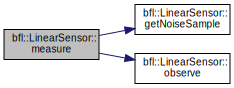
\includegraphics[width=306pt]{classbfl_1_1LinearSensor_a36f36ae6b935a8c535b553ff6a265f6a_cgraph}
\end{center}
\end{figure}
\mbox{\Hypertarget{classbfl_1_1LinearSensor_ae53acb6051164c0bcd32d5a6f88e5962}\label{classbfl_1_1LinearSensor_ae53acb6051164c0bcd32d5a6f88e5962}} 
\index{bfl\+::\+Linear\+Sensor@{bfl\+::\+Linear\+Sensor}!observe@{observe}}
\index{observe@{observe}!bfl\+::\+Linear\+Sensor@{bfl\+::\+Linear\+Sensor}}
\subsubsection{\texorpdfstring{observe()}{observe()}}
{\footnotesize\ttfamily void Linear\+Sensor\+::observe (\begin{DoxyParamCaption}\item[{const Eigen\+::\+Ref$<$ const Eigen\+::\+Matrix\+Xf $>$ \&}]{cur\+\_\+states,  }\item[{Eigen\+::\+Ref$<$ Eigen\+::\+Matrix\+Xf $>$}]{observations }\end{DoxyParamCaption})\hspace{0.3cm}{\ttfamily [override]}, {\ttfamily [virtual]}}



Implements \mbox{\hyperlink{classbfl_1_1ObservationModel_a2dd06fa6df453e491e1ab73e46f33d18}{bfl\+::\+Observation\+Model}}.



Definition at line 94 of file Linear\+Sensor.\+cpp.



References H\+\_\+.



Referenced by measure().

\mbox{\Hypertarget{classbfl_1_1LinearSensor_a83054bf80986f7b1772e71fdb8b37040}\label{classbfl_1_1LinearSensor_a83054bf80986f7b1772e71fdb8b37040}} 
\index{bfl\+::\+Linear\+Sensor@{bfl\+::\+Linear\+Sensor}!operator=@{operator=}}
\index{operator=@{operator=}!bfl\+::\+Linear\+Sensor@{bfl\+::\+Linear\+Sensor}}
\subsubsection{\texorpdfstring{operator=()}{operator=()}\hspace{0.1cm}{\footnotesize\ttfamily [1/2]}}
{\footnotesize\ttfamily \mbox{\hyperlink{classbfl_1_1LinearSensor}{Linear\+Sensor}} \& Linear\+Sensor\+::operator= (\begin{DoxyParamCaption}\item[{const \mbox{\hyperlink{classbfl_1_1LinearSensor}{Linear\+Sensor}} \&}]{lin\+\_\+sense }\end{DoxyParamCaption})\hspace{0.3cm}{\ttfamily [noexcept]}}



Definition at line 66 of file Linear\+Sensor.\+cpp.

\mbox{\Hypertarget{classbfl_1_1LinearSensor_aa93327ef56a19a9712f736d12fbf2651}\label{classbfl_1_1LinearSensor_aa93327ef56a19a9712f736d12fbf2651}} 
\index{bfl\+::\+Linear\+Sensor@{bfl\+::\+Linear\+Sensor}!operator=@{operator=}}
\index{operator=@{operator=}!bfl\+::\+Linear\+Sensor@{bfl\+::\+Linear\+Sensor}}
\subsubsection{\texorpdfstring{operator=()}{operator=()}\hspace{0.1cm}{\footnotesize\ttfamily [2/2]}}
{\footnotesize\ttfamily \mbox{\hyperlink{classbfl_1_1LinearSensor}{Linear\+Sensor}} \& Linear\+Sensor\+::operator= (\begin{DoxyParamCaption}\item[{\mbox{\hyperlink{classbfl_1_1LinearSensor}{Linear\+Sensor}} \&\&}]{lin\+\_\+sense }\end{DoxyParamCaption})\hspace{0.3cm}{\ttfamily [noexcept]}}



Definition at line 75 of file Linear\+Sensor.\+cpp.



References sigma\+\_\+x\+\_\+.

\mbox{\Hypertarget{classbfl_1_1LinearSensor_a3d20baf95d4ea62c536c87e68238852f}\label{classbfl_1_1LinearSensor_a3d20baf95d4ea62c536c87e68238852f}} 
\index{bfl\+::\+Linear\+Sensor@{bfl\+::\+Linear\+Sensor}!set\+Property@{set\+Property}}
\index{set\+Property@{set\+Property}!bfl\+::\+Linear\+Sensor@{bfl\+::\+Linear\+Sensor}}
\subsubsection{\texorpdfstring{set\+Property()}{setProperty()}}
{\footnotesize\ttfamily bool bfl\+::\+Linear\+Sensor\+::set\+Property (\begin{DoxyParamCaption}\item[{const std\+::string}]{property }\end{DoxyParamCaption})\hspace{0.3cm}{\ttfamily [inline]}, {\ttfamily [override]}, {\ttfamily [virtual]}}



Implements \mbox{\hyperlink{classbfl_1_1ObservationModel_a05991496674f63b6ea6c8a34da34194d}{bfl\+::\+Observation\+Model}}.



Definition at line 41 of file Linear\+Sensor.\+h.



\subsection{Member Data Documentation}
\mbox{\Hypertarget{classbfl_1_1LinearSensor_a5ef72350f0591e2f95d80cf5818a5366}\label{classbfl_1_1LinearSensor_a5ef72350f0591e2f95d80cf5818a5366}} 
\index{bfl\+::\+Linear\+Sensor@{bfl\+::\+Linear\+Sensor}!distribution\+\_\+@{distribution\+\_\+}}
\index{distribution\+\_\+@{distribution\+\_\+}!bfl\+::\+Linear\+Sensor@{bfl\+::\+Linear\+Sensor}}
\subsubsection{\texorpdfstring{distribution\+\_\+}{distribution\_}}
{\footnotesize\ttfamily std\+::normal\+\_\+distribution$<$float$>$ bfl\+::\+Linear\+Sensor\+::distribution\+\_\+\hspace{0.3cm}{\ttfamily [protected]}}



Definition at line 51 of file Linear\+Sensor.\+h.

\mbox{\Hypertarget{classbfl_1_1LinearSensor_a9c3d6ac31fc2aeade2d47cf0c9677cb1}\label{classbfl_1_1LinearSensor_a9c3d6ac31fc2aeade2d47cf0c9677cb1}} 
\index{bfl\+::\+Linear\+Sensor@{bfl\+::\+Linear\+Sensor}!gauss\+\_\+rnd\+\_\+sample\+\_\+@{gauss\+\_\+rnd\+\_\+sample\+\_\+}}
\index{gauss\+\_\+rnd\+\_\+sample\+\_\+@{gauss\+\_\+rnd\+\_\+sample\+\_\+}!bfl\+::\+Linear\+Sensor@{bfl\+::\+Linear\+Sensor}}
\subsubsection{\texorpdfstring{gauss\+\_\+rnd\+\_\+sample\+\_\+}{gauss\_rnd\_sample\_}}
{\footnotesize\ttfamily std\+::function$<$float()$>$ bfl\+::\+Linear\+Sensor\+::gauss\+\_\+rnd\+\_\+sample\+\_\+\hspace{0.3cm}{\ttfamily [protected]}}



Definition at line 52 of file Linear\+Sensor.\+h.



Referenced by get\+Noise\+Sample().

\mbox{\Hypertarget{classbfl_1_1LinearSensor_a564abeae2ab7fb98886f0a7952181a75}\label{classbfl_1_1LinearSensor_a564abeae2ab7fb98886f0a7952181a75}} 
\index{bfl\+::\+Linear\+Sensor@{bfl\+::\+Linear\+Sensor}!generator\+\_\+@{generator\+\_\+}}
\index{generator\+\_\+@{generator\+\_\+}!bfl\+::\+Linear\+Sensor@{bfl\+::\+Linear\+Sensor}}
\subsubsection{\texorpdfstring{generator\+\_\+}{generator\_}}
{\footnotesize\ttfamily std\+::mt19937\+\_\+64 bfl\+::\+Linear\+Sensor\+::generator\+\_\+\hspace{0.3cm}{\ttfamily [protected]}}



Definition at line 50 of file Linear\+Sensor.\+h.

\mbox{\Hypertarget{classbfl_1_1LinearSensor_ae6df14a628525b334062c104e85df7ff}\label{classbfl_1_1LinearSensor_ae6df14a628525b334062c104e85df7ff}} 
\index{bfl\+::\+Linear\+Sensor@{bfl\+::\+Linear\+Sensor}!H\+\_\+@{H\+\_\+}}
\index{H\+\_\+@{H\+\_\+}!bfl\+::\+Linear\+Sensor@{bfl\+::\+Linear\+Sensor}}
\subsubsection{\texorpdfstring{H\+\_\+}{H\_}}
{\footnotesize\ttfamily Eigen\+::\+Matrix\+Xf bfl\+::\+Linear\+Sensor\+::\+H\+\_\+\hspace{0.3cm}{\ttfamily [protected]}}



Definition at line 46 of file Linear\+Sensor.\+h.



Referenced by observe().

\mbox{\Hypertarget{classbfl_1_1LinearSensor_a3c8550ed25965c8e946a77602e44d87b}\label{classbfl_1_1LinearSensor_a3c8550ed25965c8e946a77602e44d87b}} 
\index{bfl\+::\+Linear\+Sensor@{bfl\+::\+Linear\+Sensor}!R\+\_\+@{R\+\_\+}}
\index{R\+\_\+@{R\+\_\+}!bfl\+::\+Linear\+Sensor@{bfl\+::\+Linear\+Sensor}}
\subsubsection{\texorpdfstring{R\+\_\+}{R\_}}
{\footnotesize\ttfamily Eigen\+::\+Matrix2f bfl\+::\+Linear\+Sensor\+::\+R\+\_\+\hspace{0.3cm}{\ttfamily [protected]}}



Definition at line 47 of file Linear\+Sensor.\+h.



Referenced by get\+Noise\+Covariance\+Matrix().

\mbox{\Hypertarget{classbfl_1_1LinearSensor_a3d9edc1da64faf44c02e6fb3b869bf3b}\label{classbfl_1_1LinearSensor_a3d9edc1da64faf44c02e6fb3b869bf3b}} 
\index{bfl\+::\+Linear\+Sensor@{bfl\+::\+Linear\+Sensor}!sigma\+\_\+x\+\_\+@{sigma\+\_\+x\+\_\+}}
\index{sigma\+\_\+x\+\_\+@{sigma\+\_\+x\+\_\+}!bfl\+::\+Linear\+Sensor@{bfl\+::\+Linear\+Sensor}}
\subsubsection{\texorpdfstring{sigma\+\_\+x\+\_\+}{sigma\_x\_}}
{\footnotesize\ttfamily float bfl\+::\+Linear\+Sensor\+::sigma\+\_\+x\+\_\+\hspace{0.3cm}{\ttfamily [protected]}}



Definition at line 41 of file Linear\+Sensor.\+h.



Referenced by operator=().

\mbox{\Hypertarget{classbfl_1_1LinearSensor_a6b017eefd02cd452f740af7ece2f0374}\label{classbfl_1_1LinearSensor_a6b017eefd02cd452f740af7ece2f0374}} 
\index{bfl\+::\+Linear\+Sensor@{bfl\+::\+Linear\+Sensor}!sigma\+\_\+y\+\_\+@{sigma\+\_\+y\+\_\+}}
\index{sigma\+\_\+y\+\_\+@{sigma\+\_\+y\+\_\+}!bfl\+::\+Linear\+Sensor@{bfl\+::\+Linear\+Sensor}}
\subsubsection{\texorpdfstring{sigma\+\_\+y\+\_\+}{sigma\_y\_}}
{\footnotesize\ttfamily float bfl\+::\+Linear\+Sensor\+::sigma\+\_\+y\+\_\+\hspace{0.3cm}{\ttfamily [protected]}}



Definition at line 45 of file Linear\+Sensor.\+h.

\mbox{\Hypertarget{classbfl_1_1LinearSensor_ac061b358b032a56844a48cb2024fe694}\label{classbfl_1_1LinearSensor_ac061b358b032a56844a48cb2024fe694}} 
\index{bfl\+::\+Linear\+Sensor@{bfl\+::\+Linear\+Sensor}!sqrt\+\_\+\+R\+\_\+@{sqrt\+\_\+\+R\+\_\+}}
\index{sqrt\+\_\+\+R\+\_\+@{sqrt\+\_\+\+R\+\_\+}!bfl\+::\+Linear\+Sensor@{bfl\+::\+Linear\+Sensor}}
\subsubsection{\texorpdfstring{sqrt\+\_\+\+R\+\_\+}{sqrt\_R\_}}
{\footnotesize\ttfamily Eigen\+::\+Matrix2f bfl\+::\+Linear\+Sensor\+::sqrt\+\_\+\+R\+\_\+\hspace{0.3cm}{\ttfamily [protected]}}



Definition at line 49 of file Linear\+Sensor.\+h.



Referenced by get\+Noise\+Sample().



The documentation for this class was generated from the following files\+:\begin{DoxyCompactItemize}
\item 
C\+:/\+Users/cfantacci/\+Git\+Hub/bayes-\/filters-\/lib/src/\+Bayes\+Filters/include/\+Bayes\+Filters/\mbox{\hyperlink{LinearSensor_8h}{Linear\+Sensor.\+h}}\item 
C\+:/\+Users/cfantacci/\+Git\+Hub/bayes-\/filters-\/lib/src/\+Bayes\+Filters/src/\mbox{\hyperlink{LinearSensor_8cpp}{Linear\+Sensor.\+cpp}}\end{DoxyCompactItemize}

\hypertarget{classbfl_1_1ObservationModel}{}\section{bfl\+:\+:Observation\+Model Class Reference}
\label{classbfl_1_1ObservationModel}\index{bfl\+::\+Observation\+Model@{bfl\+::\+Observation\+Model}}


{\ttfamily \#include $<$Observation\+Model.\+h$>$}



Inheritance diagram for bfl\+:\+:Observation\+Model\+:
\nopagebreak
\begin{figure}[H]
\begin{center}
\leavevmode
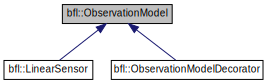
\includegraphics[width=340pt]{classbfl_1_1ObservationModel__inherit__graph}
\end{center}
\end{figure}
\subsection*{Public Member Functions}
\begin{DoxyCompactItemize}
\item 
virtual \mbox{\hyperlink{classbfl_1_1ObservationModel_ab4033bc78992bb350c9102f5e9d2fbc9}{$\sim$\+Observation\+Model}} () noexcept
\item 
virtual void \mbox{\hyperlink{classbfl_1_1ObservationModel_a2dd06fa6df453e491e1ab73e46f33d18}{observe}} (const Eigen\+::\+Ref$<$ const Eigen\+::\+Matrix\+Xf $>$ \&cur\+\_\+states, Eigen\+::\+Ref$<$ Eigen\+::\+Matrix\+Xf $>$ observations)=0
\item 
virtual void \mbox{\hyperlink{classbfl_1_1ObservationModel_a0cde643e52b6c24d80d1b49e1b58f4c0}{measure}} (const Eigen\+::\+Ref$<$ const Eigen\+::\+Matrix\+Xf $>$ \&cur\+\_\+states, Eigen\+::\+Ref$<$ Eigen\+::\+Matrix\+Xf $>$ measurements)=0
\item 
virtual Eigen\+::\+Matrix\+Xf \mbox{\hyperlink{classbfl_1_1ObservationModel_a45e8cec2a18ef49bf586c8895c13a31b}{get\+Noise\+Sample}} (const int num)=0
\item 
virtual Eigen\+::\+Matrix\+Xf \mbox{\hyperlink{classbfl_1_1ObservationModel_a63357b1456a4a5387e55d31ddb0b9b50}{get\+Noise\+Covariance\+Matrix}} ()=0
\item 
virtual bool \mbox{\hyperlink{classbfl_1_1ObservationModel_a05991496674f63b6ea6c8a34da34194d}{set\+Property}} (const std\+::string property)=0
\end{DoxyCompactItemize}


\subsection{Detailed Description}


Definition at line 12 of file Observation\+Model.\+h.



\subsection{Constructor \& Destructor Documentation}
\mbox{\Hypertarget{classbfl_1_1ObservationModel_ab4033bc78992bb350c9102f5e9d2fbc9}\label{classbfl_1_1ObservationModel_ab4033bc78992bb350c9102f5e9d2fbc9}} 
\index{bfl\+::\+Observation\+Model@{bfl\+::\+Observation\+Model}!````~Observation\+Model@{$\sim$\+Observation\+Model}}
\index{````~Observation\+Model@{$\sim$\+Observation\+Model}!bfl\+::\+Observation\+Model@{bfl\+::\+Observation\+Model}}
\subsubsection{\texorpdfstring{$\sim$\+Observation\+Model()}{~ObservationModel()}}
{\footnotesize\ttfamily virtual bfl\+::\+Observation\+Model\+::$\sim$\+Observation\+Model (\begin{DoxyParamCaption}{ }\end{DoxyParamCaption})\hspace{0.3cm}{\ttfamily [inline]}, {\ttfamily [virtual]}, {\ttfamily [noexcept]}}



Definition at line 15 of file Observation\+Model.\+h.



\subsection{Member Function Documentation}
\mbox{\Hypertarget{classbfl_1_1ObservationModel_a63357b1456a4a5387e55d31ddb0b9b50}\label{classbfl_1_1ObservationModel_a63357b1456a4a5387e55d31ddb0b9b50}} 
\index{bfl\+::\+Observation\+Model@{bfl\+::\+Observation\+Model}!get\+Noise\+Covariance\+Matrix@{get\+Noise\+Covariance\+Matrix}}
\index{get\+Noise\+Covariance\+Matrix@{get\+Noise\+Covariance\+Matrix}!bfl\+::\+Observation\+Model@{bfl\+::\+Observation\+Model}}
\subsubsection{\texorpdfstring{get\+Noise\+Covariance\+Matrix()}{getNoiseCovarianceMatrix()}}
{\footnotesize\ttfamily virtual Eigen\+::\+Matrix\+Xf bfl\+::\+Observation\+Model\+::get\+Noise\+Covariance\+Matrix (\begin{DoxyParamCaption}{ }\end{DoxyParamCaption})\hspace{0.3cm}{\ttfamily [pure virtual]}}



Implemented in \mbox{\hyperlink{classbfl_1_1LinearSensor_a7773e8de7eb58b07b1ca781b20d8537e}{bfl\+::\+Linear\+Sensor}}, and \mbox{\hyperlink{classbfl_1_1ObservationModelDecorator_a60faf028d6c83e02cf0a88c58064abf2}{bfl\+::\+Observation\+Model\+Decorator}}.

\mbox{\Hypertarget{classbfl_1_1ObservationModel_a45e8cec2a18ef49bf586c8895c13a31b}\label{classbfl_1_1ObservationModel_a45e8cec2a18ef49bf586c8895c13a31b}} 
\index{bfl\+::\+Observation\+Model@{bfl\+::\+Observation\+Model}!get\+Noise\+Sample@{get\+Noise\+Sample}}
\index{get\+Noise\+Sample@{get\+Noise\+Sample}!bfl\+::\+Observation\+Model@{bfl\+::\+Observation\+Model}}
\subsubsection{\texorpdfstring{get\+Noise\+Sample()}{getNoiseSample()}}
{\footnotesize\ttfamily virtual Eigen\+::\+Matrix\+Xf bfl\+::\+Observation\+Model\+::get\+Noise\+Sample (\begin{DoxyParamCaption}\item[{const int}]{num }\end{DoxyParamCaption})\hspace{0.3cm}{\ttfamily [pure virtual]}}



Implemented in \mbox{\hyperlink{classbfl_1_1LinearSensor_a5079f70d2a2995cff4ad3210dd1795f7}{bfl\+::\+Linear\+Sensor}}, and \mbox{\hyperlink{classbfl_1_1ObservationModelDecorator_a3e8cecfbd2402944d1f9e4682d5fd9a0}{bfl\+::\+Observation\+Model\+Decorator}}.

\mbox{\Hypertarget{classbfl_1_1ObservationModel_a0cde643e52b6c24d80d1b49e1b58f4c0}\label{classbfl_1_1ObservationModel_a0cde643e52b6c24d80d1b49e1b58f4c0}} 
\index{bfl\+::\+Observation\+Model@{bfl\+::\+Observation\+Model}!measure@{measure}}
\index{measure@{measure}!bfl\+::\+Observation\+Model@{bfl\+::\+Observation\+Model}}
\subsubsection{\texorpdfstring{measure()}{measure()}}
{\footnotesize\ttfamily virtual void bfl\+::\+Observation\+Model\+::measure (\begin{DoxyParamCaption}\item[{const Eigen\+::\+Ref$<$ const Eigen\+::\+Matrix\+Xf $>$ \&}]{cur\+\_\+states,  }\item[{Eigen\+::\+Ref$<$ Eigen\+::\+Matrix\+Xf $>$}]{measurements }\end{DoxyParamCaption})\hspace{0.3cm}{\ttfamily [pure virtual]}}



Implemented in \mbox{\hyperlink{classbfl_1_1LinearSensor_a36f36ae6b935a8c535b553ff6a265f6a}{bfl\+::\+Linear\+Sensor}}, and \mbox{\hyperlink{classbfl_1_1ObservationModelDecorator_a6b0da9bcfe0fd1beb119c79f83f8cc9a}{bfl\+::\+Observation\+Model\+Decorator}}.

\mbox{\Hypertarget{classbfl_1_1ObservationModel_a2dd06fa6df453e491e1ab73e46f33d18}\label{classbfl_1_1ObservationModel_a2dd06fa6df453e491e1ab73e46f33d18}} 
\index{bfl\+::\+Observation\+Model@{bfl\+::\+Observation\+Model}!observe@{observe}}
\index{observe@{observe}!bfl\+::\+Observation\+Model@{bfl\+::\+Observation\+Model}}
\subsubsection{\texorpdfstring{observe()}{observe()}}
{\footnotesize\ttfamily virtual void bfl\+::\+Observation\+Model\+::observe (\begin{DoxyParamCaption}\item[{const Eigen\+::\+Ref$<$ const Eigen\+::\+Matrix\+Xf $>$ \&}]{cur\+\_\+states,  }\item[{Eigen\+::\+Ref$<$ Eigen\+::\+Matrix\+Xf $>$}]{observations }\end{DoxyParamCaption})\hspace{0.3cm}{\ttfamily [pure virtual]}}



Implemented in \mbox{\hyperlink{classbfl_1_1LinearSensor_ae53acb6051164c0bcd32d5a6f88e5962}{bfl\+::\+Linear\+Sensor}}, and \mbox{\hyperlink{classbfl_1_1ObservationModelDecorator_aa2b83722ba591ab268def7a39e4e16b0}{bfl\+::\+Observation\+Model\+Decorator}}.

\mbox{\Hypertarget{classbfl_1_1ObservationModel_a05991496674f63b6ea6c8a34da34194d}\label{classbfl_1_1ObservationModel_a05991496674f63b6ea6c8a34da34194d}} 
\index{bfl\+::\+Observation\+Model@{bfl\+::\+Observation\+Model}!set\+Property@{set\+Property}}
\index{set\+Property@{set\+Property}!bfl\+::\+Observation\+Model@{bfl\+::\+Observation\+Model}}
\subsubsection{\texorpdfstring{set\+Property()}{setProperty()}}
{\footnotesize\ttfamily virtual bool bfl\+::\+Observation\+Model\+::set\+Property (\begin{DoxyParamCaption}\item[{const std\+::string}]{property }\end{DoxyParamCaption})\hspace{0.3cm}{\ttfamily [pure virtual]}}



Implemented in \mbox{\hyperlink{classbfl_1_1LinearSensor_a3d20baf95d4ea62c536c87e68238852f}{bfl\+::\+Linear\+Sensor}}, and \mbox{\hyperlink{classbfl_1_1ObservationModelDecorator_a0d6ab787754a56159e3d1bc6d56a961c}{bfl\+::\+Observation\+Model\+Decorator}}.



The documentation for this class was generated from the following file\+:\begin{DoxyCompactItemize}
\item 
C\+:/\+Users/cfantacci/\+Git\+Hub/bayes-\/filters-\/lib/src/\+Bayes\+Filters/include/\+Bayes\+Filters/\mbox{\hyperlink{ObservationModel_8h}{Observation\+Model.\+h}}\end{DoxyCompactItemize}

\hypertarget{classbfl_1_1ObservationModelDecorator}{}\section{bfl\+:\+:Observation\+Model\+Decorator Class Reference}
\label{classbfl_1_1ObservationModelDecorator}\index{bfl\+::\+Observation\+Model\+Decorator@{bfl\+::\+Observation\+Model\+Decorator}}


{\ttfamily \#include $<$Observation\+Model\+Decorator.\+h$>$}



Inheritance diagram for bfl\+:\+:Observation\+Model\+Decorator\+:
\nopagebreak
\begin{figure}[H]
\begin{center}
\leavevmode
\includegraphics[width=232pt]{classbfl_1_1ObservationModelDecorator__inherit__graph}
\end{center}
\end{figure}
\subsection*{Public Member Functions}
\begin{DoxyCompactItemize}
\item 
void \mbox{\hyperlink{classbfl_1_1ObservationModelDecorator_aa2b83722ba591ab268def7a39e4e16b0}{observe}} (const Eigen\+::\+Ref$<$ const Eigen\+::\+Matrix\+Xf $>$ \&cur\+\_\+states, Eigen\+::\+Ref$<$ Eigen\+::\+Matrix\+Xf $>$ observations) override
\item 
void \mbox{\hyperlink{classbfl_1_1ObservationModelDecorator_a6b0da9bcfe0fd1beb119c79f83f8cc9a}{measure}} (const Eigen\+::\+Ref$<$ const Eigen\+::\+Matrix\+Xf $>$ \&cur\+\_\+states, Eigen\+::\+Ref$<$ Eigen\+::\+Matrix\+Xf $>$ measurements) override
\item 
Eigen\+::\+Matrix\+Xf \mbox{\hyperlink{classbfl_1_1ObservationModelDecorator_a3e8cecfbd2402944d1f9e4682d5fd9a0}{get\+Noise\+Sample}} (const int num) override
\item 
Eigen\+::\+Matrix\+Xf \mbox{\hyperlink{classbfl_1_1ObservationModelDecorator_a60faf028d6c83e02cf0a88c58064abf2}{get\+Noise\+Covariance\+Matrix}} () override
\item 
bool \mbox{\hyperlink{classbfl_1_1ObservationModelDecorator_a0d6ab787754a56159e3d1bc6d56a961c}{set\+Property}} (const std\+::string property) override
\end{DoxyCompactItemize}
\subsection*{Protected Member Functions}
\begin{DoxyCompactItemize}
\item 
\mbox{\hyperlink{classbfl_1_1ObservationModelDecorator_ac48b0ef08d89cfddb689e0ecef2cb0f9}{Observation\+Model\+Decorator}} (std\+::unique\+\_\+ptr$<$ \mbox{\hyperlink{classbfl_1_1ObservationModel}{Observation\+Model}} $>$ observation\+\_\+model) noexcept
\item 
\mbox{\hyperlink{classbfl_1_1ObservationModelDecorator_a7ab0e6fdcd159a52886559e22ac475ba}{Observation\+Model\+Decorator}} (\mbox{\hyperlink{classbfl_1_1ObservationModelDecorator}{Observation\+Model\+Decorator}} \&\&observation\+\_\+model) noexcept
\item 
virtual \mbox{\hyperlink{classbfl_1_1ObservationModelDecorator_a3bad5ad9085e34b71557d9444c6280f4}{$\sim$\+Observation\+Model\+Decorator}} () noexcept
\item 
\mbox{\hyperlink{classbfl_1_1ObservationModelDecorator}{Observation\+Model\+Decorator}} \& \mbox{\hyperlink{classbfl_1_1ObservationModelDecorator_ade8f68b2598a40e9db26fcdbc0aa6638}{operator=}} (\mbox{\hyperlink{classbfl_1_1ObservationModelDecorator}{Observation\+Model\+Decorator}} \&\&observation\+\_\+model) noexcept
\end{DoxyCompactItemize}
\subsection*{Private Attributes}
\begin{DoxyCompactItemize}
\item 
std\+::unique\+\_\+ptr$<$ \mbox{\hyperlink{classbfl_1_1ObservationModel}{Observation\+Model}} $>$ \mbox{\hyperlink{classbfl_1_1ObservationModelDecorator_abec4efacd0bb8e55bb9a6aade1bb28ad}{observation\+\_\+model\+\_\+}}
\end{DoxyCompactItemize}


\subsection{Detailed Description}


Definition at line 13 of file Observation\+Model\+Decorator.\+h.



\subsection{Constructor \& Destructor Documentation}
\mbox{\Hypertarget{classbfl_1_1ObservationModelDecorator_ac48b0ef08d89cfddb689e0ecef2cb0f9}\label{classbfl_1_1ObservationModelDecorator_ac48b0ef08d89cfddb689e0ecef2cb0f9}} 
\index{bfl\+::\+Observation\+Model\+Decorator@{bfl\+::\+Observation\+Model\+Decorator}!Observation\+Model\+Decorator@{Observation\+Model\+Decorator}}
\index{Observation\+Model\+Decorator@{Observation\+Model\+Decorator}!bfl\+::\+Observation\+Model\+Decorator@{bfl\+::\+Observation\+Model\+Decorator}}
\subsubsection{\texorpdfstring{Observation\+Model\+Decorator()}{ObservationModelDecorator()}\hspace{0.1cm}{\footnotesize\ttfamily [1/2]}}
{\footnotesize\ttfamily Observation\+Model\+Decorator\+::\+Observation\+Model\+Decorator (\begin{DoxyParamCaption}\item[{std\+::unique\+\_\+ptr$<$ \mbox{\hyperlink{classbfl_1_1ObservationModel}{Observation\+Model}} $>$}]{observation\+\_\+model }\end{DoxyParamCaption})\hspace{0.3cm}{\ttfamily [protected]}, {\ttfamily [noexcept]}}



Definition at line 7 of file Observation\+Model\+Decorator.\+cpp.

\mbox{\Hypertarget{classbfl_1_1ObservationModelDecorator_a7ab0e6fdcd159a52886559e22ac475ba}\label{classbfl_1_1ObservationModelDecorator_a7ab0e6fdcd159a52886559e22ac475ba}} 
\index{bfl\+::\+Observation\+Model\+Decorator@{bfl\+::\+Observation\+Model\+Decorator}!Observation\+Model\+Decorator@{Observation\+Model\+Decorator}}
\index{Observation\+Model\+Decorator@{Observation\+Model\+Decorator}!bfl\+::\+Observation\+Model\+Decorator@{bfl\+::\+Observation\+Model\+Decorator}}
\subsubsection{\texorpdfstring{Observation\+Model\+Decorator()}{ObservationModelDecorator()}\hspace{0.1cm}{\footnotesize\ttfamily [2/2]}}
{\footnotesize\ttfamily Observation\+Model\+Decorator\+::\+Observation\+Model\+Decorator (\begin{DoxyParamCaption}\item[{\mbox{\hyperlink{classbfl_1_1ObservationModelDecorator}{Observation\+Model\+Decorator}} \&\&}]{observation\+\_\+model }\end{DoxyParamCaption})\hspace{0.3cm}{\ttfamily [protected]}, {\ttfamily [noexcept]}}



Definition at line 11 of file Observation\+Model\+Decorator.\+cpp.

\mbox{\Hypertarget{classbfl_1_1ObservationModelDecorator_a3bad5ad9085e34b71557d9444c6280f4}\label{classbfl_1_1ObservationModelDecorator_a3bad5ad9085e34b71557d9444c6280f4}} 
\index{bfl\+::\+Observation\+Model\+Decorator@{bfl\+::\+Observation\+Model\+Decorator}!````~Observation\+Model\+Decorator@{$\sim$\+Observation\+Model\+Decorator}}
\index{````~Observation\+Model\+Decorator@{$\sim$\+Observation\+Model\+Decorator}!bfl\+::\+Observation\+Model\+Decorator@{bfl\+::\+Observation\+Model\+Decorator}}
\subsubsection{\texorpdfstring{$\sim$\+Observation\+Model\+Decorator()}{~ObservationModelDecorator()}}
{\footnotesize\ttfamily Observation\+Model\+Decorator\+::$\sim$\+Observation\+Model\+Decorator (\begin{DoxyParamCaption}{ }\end{DoxyParamCaption})\hspace{0.3cm}{\ttfamily [protected]}, {\ttfamily [virtual]}, {\ttfamily [noexcept]}}



Definition at line 15 of file Observation\+Model\+Decorator.\+cpp.



\subsection{Member Function Documentation}
\mbox{\Hypertarget{classbfl_1_1ObservationModelDecorator_a60faf028d6c83e02cf0a88c58064abf2}\label{classbfl_1_1ObservationModelDecorator_a60faf028d6c83e02cf0a88c58064abf2}} 
\index{bfl\+::\+Observation\+Model\+Decorator@{bfl\+::\+Observation\+Model\+Decorator}!get\+Noise\+Covariance\+Matrix@{get\+Noise\+Covariance\+Matrix}}
\index{get\+Noise\+Covariance\+Matrix@{get\+Noise\+Covariance\+Matrix}!bfl\+::\+Observation\+Model\+Decorator@{bfl\+::\+Observation\+Model\+Decorator}}
\subsubsection{\texorpdfstring{get\+Noise\+Covariance\+Matrix()}{getNoiseCovarianceMatrix()}}
{\footnotesize\ttfamily Matrix\+Xf Observation\+Model\+Decorator\+::get\+Noise\+Covariance\+Matrix (\begin{DoxyParamCaption}{ }\end{DoxyParamCaption})\hspace{0.3cm}{\ttfamily [override]}, {\ttfamily [virtual]}}



Implements \mbox{\hyperlink{classbfl_1_1ObservationModel_a63357b1456a4a5387e55d31ddb0b9b50}{bfl\+::\+Observation\+Model}}.



Definition at line 44 of file Observation\+Model\+Decorator.\+cpp.

\mbox{\Hypertarget{classbfl_1_1ObservationModelDecorator_a3e8cecfbd2402944d1f9e4682d5fd9a0}\label{classbfl_1_1ObservationModelDecorator_a3e8cecfbd2402944d1f9e4682d5fd9a0}} 
\index{bfl\+::\+Observation\+Model\+Decorator@{bfl\+::\+Observation\+Model\+Decorator}!get\+Noise\+Sample@{get\+Noise\+Sample}}
\index{get\+Noise\+Sample@{get\+Noise\+Sample}!bfl\+::\+Observation\+Model\+Decorator@{bfl\+::\+Observation\+Model\+Decorator}}
\subsubsection{\texorpdfstring{get\+Noise\+Sample()}{getNoiseSample()}}
{\footnotesize\ttfamily Matrix\+Xf Observation\+Model\+Decorator\+::get\+Noise\+Sample (\begin{DoxyParamCaption}\item[{const int}]{num }\end{DoxyParamCaption})\hspace{0.3cm}{\ttfamily [override]}, {\ttfamily [virtual]}}



Implements \mbox{\hyperlink{classbfl_1_1ObservationModel_a45e8cec2a18ef49bf586c8895c13a31b}{bfl\+::\+Observation\+Model}}.



Definition at line 38 of file Observation\+Model\+Decorator.\+cpp.

\mbox{\Hypertarget{classbfl_1_1ObservationModelDecorator_a6b0da9bcfe0fd1beb119c79f83f8cc9a}\label{classbfl_1_1ObservationModelDecorator_a6b0da9bcfe0fd1beb119c79f83f8cc9a}} 
\index{bfl\+::\+Observation\+Model\+Decorator@{bfl\+::\+Observation\+Model\+Decorator}!measure@{measure}}
\index{measure@{measure}!bfl\+::\+Observation\+Model\+Decorator@{bfl\+::\+Observation\+Model\+Decorator}}
\subsubsection{\texorpdfstring{measure()}{measure()}}
{\footnotesize\ttfamily void Observation\+Model\+Decorator\+::measure (\begin{DoxyParamCaption}\item[{const Eigen\+::\+Ref$<$ const Eigen\+::\+Matrix\+Xf $>$ \&}]{cur\+\_\+states,  }\item[{Eigen\+::\+Ref$<$ Eigen\+::\+Matrix\+Xf $>$}]{measurements }\end{DoxyParamCaption})\hspace{0.3cm}{\ttfamily [override]}, {\ttfamily [virtual]}}



Implements \mbox{\hyperlink{classbfl_1_1ObservationModel_a0cde643e52b6c24d80d1b49e1b58f4c0}{bfl\+::\+Observation\+Model}}.



Definition at line 32 of file Observation\+Model\+Decorator.\+cpp.

\mbox{\Hypertarget{classbfl_1_1ObservationModelDecorator_aa2b83722ba591ab268def7a39e4e16b0}\label{classbfl_1_1ObservationModelDecorator_aa2b83722ba591ab268def7a39e4e16b0}} 
\index{bfl\+::\+Observation\+Model\+Decorator@{bfl\+::\+Observation\+Model\+Decorator}!observe@{observe}}
\index{observe@{observe}!bfl\+::\+Observation\+Model\+Decorator@{bfl\+::\+Observation\+Model\+Decorator}}
\subsubsection{\texorpdfstring{observe()}{observe()}}
{\footnotesize\ttfamily void Observation\+Model\+Decorator\+::observe (\begin{DoxyParamCaption}\item[{const Eigen\+::\+Ref$<$ const Eigen\+::\+Matrix\+Xf $>$ \&}]{cur\+\_\+states,  }\item[{Eigen\+::\+Ref$<$ Eigen\+::\+Matrix\+Xf $>$}]{observations }\end{DoxyParamCaption})\hspace{0.3cm}{\ttfamily [override]}, {\ttfamily [virtual]}}



Implements \mbox{\hyperlink{classbfl_1_1ObservationModel_a2dd06fa6df453e491e1ab73e46f33d18}{bfl\+::\+Observation\+Model}}.



Definition at line 26 of file Observation\+Model\+Decorator.\+cpp.

\mbox{\Hypertarget{classbfl_1_1ObservationModelDecorator_ade8f68b2598a40e9db26fcdbc0aa6638}\label{classbfl_1_1ObservationModelDecorator_ade8f68b2598a40e9db26fcdbc0aa6638}} 
\index{bfl\+::\+Observation\+Model\+Decorator@{bfl\+::\+Observation\+Model\+Decorator}!operator=@{operator=}}
\index{operator=@{operator=}!bfl\+::\+Observation\+Model\+Decorator@{bfl\+::\+Observation\+Model\+Decorator}}
\subsubsection{\texorpdfstring{operator=()}{operator=()}}
{\footnotesize\ttfamily \mbox{\hyperlink{classbfl_1_1ObservationModelDecorator}{Observation\+Model\+Decorator}} \& Observation\+Model\+Decorator\+::operator= (\begin{DoxyParamCaption}\item[{\mbox{\hyperlink{classbfl_1_1ObservationModelDecorator}{Observation\+Model\+Decorator}} \&\&}]{observation\+\_\+model }\end{DoxyParamCaption})\hspace{0.3cm}{\ttfamily [protected]}, {\ttfamily [noexcept]}}



Definition at line 18 of file Observation\+Model\+Decorator.\+cpp.

\mbox{\Hypertarget{classbfl_1_1ObservationModelDecorator_a0d6ab787754a56159e3d1bc6d56a961c}\label{classbfl_1_1ObservationModelDecorator_a0d6ab787754a56159e3d1bc6d56a961c}} 
\index{bfl\+::\+Observation\+Model\+Decorator@{bfl\+::\+Observation\+Model\+Decorator}!set\+Property@{set\+Property}}
\index{set\+Property@{set\+Property}!bfl\+::\+Observation\+Model\+Decorator@{bfl\+::\+Observation\+Model\+Decorator}}
\subsubsection{\texorpdfstring{set\+Property()}{setProperty()}}
{\footnotesize\ttfamily bool Observation\+Model\+Decorator\+::set\+Property (\begin{DoxyParamCaption}\item[{const std\+::string}]{property }\end{DoxyParamCaption})\hspace{0.3cm}{\ttfamily [override]}, {\ttfamily [virtual]}}



Implements \mbox{\hyperlink{classbfl_1_1ObservationModel_a05991496674f63b6ea6c8a34da34194d}{bfl\+::\+Observation\+Model}}.



Definition at line 50 of file Observation\+Model\+Decorator.\+cpp.



\subsection{Member Data Documentation}
\mbox{\Hypertarget{classbfl_1_1ObservationModelDecorator_abec4efacd0bb8e55bb9a6aade1bb28ad}\label{classbfl_1_1ObservationModelDecorator_abec4efacd0bb8e55bb9a6aade1bb28ad}} 
\index{bfl\+::\+Observation\+Model\+Decorator@{bfl\+::\+Observation\+Model\+Decorator}!observation\+\_\+model\+\_\+@{observation\+\_\+model\+\_\+}}
\index{observation\+\_\+model\+\_\+@{observation\+\_\+model\+\_\+}!bfl\+::\+Observation\+Model\+Decorator@{bfl\+::\+Observation\+Model\+Decorator}}
\subsubsection{\texorpdfstring{observation\+\_\+model\+\_\+}{observation\_model\_}}
{\footnotesize\ttfamily std\+::unique\+\_\+ptr$<$\mbox{\hyperlink{classbfl_1_1ObservationModel}{Observation\+Model}}$>$ bfl\+::\+Observation\+Model\+Decorator\+::observation\+\_\+model\+\_\+\hspace{0.3cm}{\ttfamily [private]}}



Definition at line 36 of file Observation\+Model\+Decorator.\+h.



The documentation for this class was generated from the following files\+:\begin{DoxyCompactItemize}
\item 
C\+:/\+Users/cfantacci/\+Git\+Hub/bayes-\/filters-\/lib/src/\+Bayes\+Filters/include/\+Bayes\+Filters/\mbox{\hyperlink{ObservationModelDecorator_8h}{Observation\+Model\+Decorator.\+h}}\item 
C\+:/\+Users/cfantacci/\+Git\+Hub/bayes-\/filters-\/lib/src/\+Bayes\+Filters/src/\mbox{\hyperlink{ObservationModelDecorator_8cpp}{Observation\+Model\+Decorator.\+cpp}}\end{DoxyCompactItemize}

\input{classbfl_1_1ParticleFilter}
\hypertarget{classbfl_1_1PFCorrection}{}\section{bfl\+:\+:P\+F\+Correction Class Reference}
\label{classbfl_1_1PFCorrection}\index{bfl\+::\+P\+F\+Correction@{bfl\+::\+P\+F\+Correction}}


{\ttfamily \#include $<$P\+F\+Correction.\+h$>$}



Inheritance diagram for bfl\+:\+:P\+F\+Correction\+:
\nopagebreak
\begin{figure}[H]
\begin{center}
\leavevmode
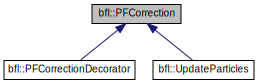
\includegraphics[width=330pt]{classbfl_1_1PFCorrection__inherit__graph}
\end{center}
\end{figure}
\subsection*{Public Member Functions}
\begin{DoxyCompactItemize}
\item 
virtual \mbox{\hyperlink{classbfl_1_1PFCorrection_aa26f1c91715ebccc1d3c25f673d32279}{$\sim$\+P\+F\+Correction}} () noexcept
\item 
void \mbox{\hyperlink{classbfl_1_1PFCorrection_a7d8e7f910fe5ebcb7d8ed678c6f38836}{correct}} (const Eigen\+::\+Ref$<$ const Eigen\+::\+Matrix\+Xf $>$ \&pred\+\_\+states, const Eigen\+::\+Ref$<$ const Eigen\+::\+Vector\+Xf $>$ \&pred\+\_\+weights, const Eigen\+::\+Ref$<$ const Eigen\+::\+Matrix\+Xf $>$ \&measurements, Eigen\+::\+Ref$<$ Eigen\+::\+Matrix\+Xf $>$ cor\+\_\+states, Eigen\+::\+Ref$<$ Eigen\+::\+Vector\+Xf $>$ cor\+\_\+weights)
\item 
virtual void \mbox{\hyperlink{classbfl_1_1PFCorrection_a22e803c147f8fb45b7b98c854a947057}{innovation}} (const Eigen\+::\+Ref$<$ const Eigen\+::\+Matrix\+Xf $>$ \&pred\+\_\+states, const Eigen\+::\+Ref$<$ const Eigen\+::\+Matrix\+Xf $>$ \&measurements, Eigen\+::\+Ref$<$ Eigen\+::\+Matrix\+Xf $>$ innovations)=0
\item 
virtual double \mbox{\hyperlink{classbfl_1_1PFCorrection_a4310e630d4c269bd66557e44e5deecb0}{likelihood}} (const Eigen\+::\+Ref$<$ const Eigen\+::\+Vector\+Xf $>$ \&\mbox{\hyperlink{classbfl_1_1PFCorrection_a22e803c147f8fb45b7b98c854a947057}{innovation}})=0
\item 
bool \mbox{\hyperlink{classbfl_1_1PFCorrection_ab25e625ea12fe257e0eb85d465835e62}{skip}} (const bool status)
\item 
virtual \mbox{\hyperlink{classbfl_1_1ObservationModel}{Observation\+Model}} \& \mbox{\hyperlink{classbfl_1_1PFCorrection_a3bc4010f306825d69014bee53cd262ad}{get\+Observation\+Model}} ()=0
\item 
virtual void \mbox{\hyperlink{classbfl_1_1PFCorrection_a437fcf552a85f427d1369d8e43e56144}{set\+Observation\+Model}} (std\+::unique\+\_\+ptr$<$ \mbox{\hyperlink{classbfl_1_1ObservationModel}{Observation\+Model}} $>$ observation\+\_\+model)=0
\end{DoxyCompactItemize}
\subsection*{Protected Member Functions}
\begin{DoxyCompactItemize}
\item 
\mbox{\hyperlink{classbfl_1_1PFCorrection_ae4be8c44771f209d79c549305cb63dcf}{P\+F\+Correction}} () noexcept
\item 
\mbox{\hyperlink{classbfl_1_1PFCorrection_a95a379a1b622c782020bdd06c59cca3f}{P\+F\+Correction}} (\mbox{\hyperlink{classbfl_1_1PFCorrection}{P\+F\+Correction}} \&\&pf\+\_\+correction) noexcept
\item 
virtual void \mbox{\hyperlink{classbfl_1_1PFCorrection_a3fb61b90d36bea3271c1c9e363c61229}{correct\+Step}} (const Eigen\+::\+Ref$<$ const Eigen\+::\+Matrix\+Xf $>$ \&pred\+\_\+states, const Eigen\+::\+Ref$<$ const Eigen\+::\+Vector\+Xf $>$ \&pred\+\_\+weights, const Eigen\+::\+Ref$<$ const Eigen\+::\+Matrix\+Xf $>$ \&measurements, Eigen\+::\+Ref$<$ Eigen\+::\+Matrix\+Xf $>$ cor\+\_\+states, Eigen\+::\+Ref$<$ Eigen\+::\+Vector\+Xf $>$ cor\+\_\+weights)=0
\end{DoxyCompactItemize}
\subsection*{Private Attributes}
\begin{DoxyCompactItemize}
\item 
bool \mbox{\hyperlink{classbfl_1_1PFCorrection_aac7b1063a3207bd00547ad5490bbc935}{skip\+\_\+}} = false
\end{DoxyCompactItemize}
\subsection*{Friends}
\begin{DoxyCompactItemize}
\item 
class \mbox{\hyperlink{classbfl_1_1PFCorrection_a58497dd469f7041f127774bccdc78022}{P\+F\+Correction\+Decorator}}
\end{DoxyCompactItemize}


\subsection{Detailed Description}


Definition at line 15 of file P\+F\+Correction.\+h.



\subsection{Constructor \& Destructor Documentation}
\mbox{\Hypertarget{classbfl_1_1PFCorrection_aa26f1c91715ebccc1d3c25f673d32279}\label{classbfl_1_1PFCorrection_aa26f1c91715ebccc1d3c25f673d32279}} 
\index{bfl\+::\+P\+F\+Correction@{bfl\+::\+P\+F\+Correction}!````~P\+F\+Correction@{$\sim$\+P\+F\+Correction}}
\index{````~P\+F\+Correction@{$\sim$\+P\+F\+Correction}!bfl\+::\+P\+F\+Correction@{bfl\+::\+P\+F\+Correction}}
\subsubsection{\texorpdfstring{$\sim$\+P\+F\+Correction()}{~PFCorrection()}}
{\footnotesize\ttfamily virtual bfl\+::\+P\+F\+Correction\+::$\sim$\+P\+F\+Correction (\begin{DoxyParamCaption}{ }\end{DoxyParamCaption})\hspace{0.3cm}{\ttfamily [inline]}, {\ttfamily [virtual]}, {\ttfamily [noexcept]}}



Definition at line 18 of file P\+F\+Correction.\+h.

\mbox{\Hypertarget{classbfl_1_1PFCorrection_ae4be8c44771f209d79c549305cb63dcf}\label{classbfl_1_1PFCorrection_ae4be8c44771f209d79c549305cb63dcf}} 
\index{bfl\+::\+P\+F\+Correction@{bfl\+::\+P\+F\+Correction}!P\+F\+Correction@{P\+F\+Correction}}
\index{P\+F\+Correction@{P\+F\+Correction}!bfl\+::\+P\+F\+Correction@{bfl\+::\+P\+F\+Correction}}
\subsubsection{\texorpdfstring{P\+F\+Correction()}{PFCorrection()}\hspace{0.1cm}{\footnotesize\ttfamily [1/2]}}
{\footnotesize\ttfamily P\+F\+Correction\+::\+P\+F\+Correction (\begin{DoxyParamCaption}{ }\end{DoxyParamCaption})\hspace{0.3cm}{\ttfamily [protected]}, {\ttfamily [noexcept]}}



Definition at line 7 of file P\+F\+Correction.\+cpp.

\mbox{\Hypertarget{classbfl_1_1PFCorrection_a95a379a1b622c782020bdd06c59cca3f}\label{classbfl_1_1PFCorrection_a95a379a1b622c782020bdd06c59cca3f}} 
\index{bfl\+::\+P\+F\+Correction@{bfl\+::\+P\+F\+Correction}!P\+F\+Correction@{P\+F\+Correction}}
\index{P\+F\+Correction@{P\+F\+Correction}!bfl\+::\+P\+F\+Correction@{bfl\+::\+P\+F\+Correction}}
\subsubsection{\texorpdfstring{P\+F\+Correction()}{PFCorrection()}\hspace{0.1cm}{\footnotesize\ttfamily [2/2]}}
{\footnotesize\ttfamily P\+F\+Correction\+::\+P\+F\+Correction (\begin{DoxyParamCaption}\item[{\mbox{\hyperlink{classbfl_1_1PFCorrection}{P\+F\+Correction}} \&\&}]{pf\+\_\+correction }\end{DoxyParamCaption})\hspace{0.3cm}{\ttfamily [protected]}, {\ttfamily [noexcept]}}



Definition at line 10 of file P\+F\+Correction.\+cpp.



\subsection{Member Function Documentation}
\mbox{\Hypertarget{classbfl_1_1PFCorrection_a7d8e7f910fe5ebcb7d8ed678c6f38836}\label{classbfl_1_1PFCorrection_a7d8e7f910fe5ebcb7d8ed678c6f38836}} 
\index{bfl\+::\+P\+F\+Correction@{bfl\+::\+P\+F\+Correction}!correct@{correct}}
\index{correct@{correct}!bfl\+::\+P\+F\+Correction@{bfl\+::\+P\+F\+Correction}}
\subsubsection{\texorpdfstring{correct()}{correct()}}
{\footnotesize\ttfamily void P\+F\+Correction\+::correct (\begin{DoxyParamCaption}\item[{const Eigen\+::\+Ref$<$ const Eigen\+::\+Matrix\+Xf $>$ \&}]{pred\+\_\+states,  }\item[{const Eigen\+::\+Ref$<$ const Eigen\+::\+Vector\+Xf $>$ \&}]{pred\+\_\+weights,  }\item[{const Eigen\+::\+Ref$<$ const Eigen\+::\+Matrix\+Xf $>$ \&}]{measurements,  }\item[{Eigen\+::\+Ref$<$ Eigen\+::\+Matrix\+Xf $>$}]{cor\+\_\+states,  }\item[{Eigen\+::\+Ref$<$ Eigen\+::\+Vector\+Xf $>$}]{cor\+\_\+weights }\end{DoxyParamCaption})}



Definition at line 17 of file P\+F\+Correction.\+cpp.

\mbox{\Hypertarget{classbfl_1_1PFCorrection_a3fb61b90d36bea3271c1c9e363c61229}\label{classbfl_1_1PFCorrection_a3fb61b90d36bea3271c1c9e363c61229}} 
\index{bfl\+::\+P\+F\+Correction@{bfl\+::\+P\+F\+Correction}!correct\+Step@{correct\+Step}}
\index{correct\+Step@{correct\+Step}!bfl\+::\+P\+F\+Correction@{bfl\+::\+P\+F\+Correction}}
\subsubsection{\texorpdfstring{correct\+Step()}{correctStep()}}
{\footnotesize\ttfamily virtual void bfl\+::\+P\+F\+Correction\+::correct\+Step (\begin{DoxyParamCaption}\item[{const Eigen\+::\+Ref$<$ const Eigen\+::\+Matrix\+Xf $>$ \&}]{pred\+\_\+states,  }\item[{const Eigen\+::\+Ref$<$ const Eigen\+::\+Vector\+Xf $>$ \&}]{pred\+\_\+weights,  }\item[{const Eigen\+::\+Ref$<$ const Eigen\+::\+Matrix\+Xf $>$ \&}]{measurements,  }\item[{Eigen\+::\+Ref$<$ Eigen\+::\+Matrix\+Xf $>$}]{cor\+\_\+states,  }\item[{Eigen\+::\+Ref$<$ Eigen\+::\+Vector\+Xf $>$}]{cor\+\_\+weights }\end{DoxyParamCaption})\hspace{0.3cm}{\ttfamily [protected]}, {\ttfamily [pure virtual]}}



Implemented in \mbox{\hyperlink{classbfl_1_1UpdateParticles_aa589f7fab7cd83f310c9dc17ee169dec}{bfl\+::\+Update\+Particles}}, and \mbox{\hyperlink{classbfl_1_1PFCorrectionDecorator_abb5ab0ef4245b67be546360a54416498}{bfl\+::\+P\+F\+Correction\+Decorator}}.

\mbox{\Hypertarget{classbfl_1_1PFCorrection_a3bc4010f306825d69014bee53cd262ad}\label{classbfl_1_1PFCorrection_a3bc4010f306825d69014bee53cd262ad}} 
\index{bfl\+::\+P\+F\+Correction@{bfl\+::\+P\+F\+Correction}!get\+Observation\+Model@{get\+Observation\+Model}}
\index{get\+Observation\+Model@{get\+Observation\+Model}!bfl\+::\+P\+F\+Correction@{bfl\+::\+P\+F\+Correction}}
\subsubsection{\texorpdfstring{get\+Observation\+Model()}{getObservationModel()}}
{\footnotesize\ttfamily virtual \mbox{\hyperlink{classbfl_1_1ObservationModel}{Observation\+Model}}\& bfl\+::\+P\+F\+Correction\+::get\+Observation\+Model (\begin{DoxyParamCaption}{ }\end{DoxyParamCaption})\hspace{0.3cm}{\ttfamily [pure virtual]}}



Implemented in \mbox{\hyperlink{classbfl_1_1UpdateParticles_a673781f8cadbd148cb9a67a3f8532b37}{bfl\+::\+Update\+Particles}}, and \mbox{\hyperlink{classbfl_1_1PFCorrectionDecorator_a7bafd701e4a97efc55ba7fea6125cc7f}{bfl\+::\+P\+F\+Correction\+Decorator}}.

\mbox{\Hypertarget{classbfl_1_1PFCorrection_a22e803c147f8fb45b7b98c854a947057}\label{classbfl_1_1PFCorrection_a22e803c147f8fb45b7b98c854a947057}} 
\index{bfl\+::\+P\+F\+Correction@{bfl\+::\+P\+F\+Correction}!innovation@{innovation}}
\index{innovation@{innovation}!bfl\+::\+P\+F\+Correction@{bfl\+::\+P\+F\+Correction}}
\subsubsection{\texorpdfstring{innovation()}{innovation()}}
{\footnotesize\ttfamily virtual void bfl\+::\+P\+F\+Correction\+::innovation (\begin{DoxyParamCaption}\item[{const Eigen\+::\+Ref$<$ const Eigen\+::\+Matrix\+Xf $>$ \&}]{pred\+\_\+states,  }\item[{const Eigen\+::\+Ref$<$ const Eigen\+::\+Matrix\+Xf $>$ \&}]{measurements,  }\item[{Eigen\+::\+Ref$<$ Eigen\+::\+Matrix\+Xf $>$}]{innovations }\end{DoxyParamCaption})\hspace{0.3cm}{\ttfamily [pure virtual]}}



Implemented in \mbox{\hyperlink{classbfl_1_1UpdateParticles_a8eb8aa7a1cbcf1b285401bc2b0dbed3e}{bfl\+::\+Update\+Particles}}, and \mbox{\hyperlink{classbfl_1_1PFCorrectionDecorator_ac468b6ca9f6991217b6771173c253b42}{bfl\+::\+P\+F\+Correction\+Decorator}}.

\mbox{\Hypertarget{classbfl_1_1PFCorrection_a4310e630d4c269bd66557e44e5deecb0}\label{classbfl_1_1PFCorrection_a4310e630d4c269bd66557e44e5deecb0}} 
\index{bfl\+::\+P\+F\+Correction@{bfl\+::\+P\+F\+Correction}!likelihood@{likelihood}}
\index{likelihood@{likelihood}!bfl\+::\+P\+F\+Correction@{bfl\+::\+P\+F\+Correction}}
\subsubsection{\texorpdfstring{likelihood()}{likelihood()}}
{\footnotesize\ttfamily virtual double bfl\+::\+P\+F\+Correction\+::likelihood (\begin{DoxyParamCaption}\item[{const Eigen\+::\+Ref$<$ const Eigen\+::\+Vector\+Xf $>$ \&}]{innovation }\end{DoxyParamCaption})\hspace{0.3cm}{\ttfamily [pure virtual]}}



Implemented in \mbox{\hyperlink{classbfl_1_1UpdateParticles_a262b9de317562f0361f2db68312b8e27}{bfl\+::\+Update\+Particles}}, and \mbox{\hyperlink{classbfl_1_1PFCorrectionDecorator_a39c3201dbd0821427b684228451faea5}{bfl\+::\+P\+F\+Correction\+Decorator}}.

\mbox{\Hypertarget{classbfl_1_1PFCorrection_a437fcf552a85f427d1369d8e43e56144}\label{classbfl_1_1PFCorrection_a437fcf552a85f427d1369d8e43e56144}} 
\index{bfl\+::\+P\+F\+Correction@{bfl\+::\+P\+F\+Correction}!set\+Observation\+Model@{set\+Observation\+Model}}
\index{set\+Observation\+Model@{set\+Observation\+Model}!bfl\+::\+P\+F\+Correction@{bfl\+::\+P\+F\+Correction}}
\subsubsection{\texorpdfstring{set\+Observation\+Model()}{setObservationModel()}}
{\footnotesize\ttfamily virtual void bfl\+::\+P\+F\+Correction\+::set\+Observation\+Model (\begin{DoxyParamCaption}\item[{std\+::unique\+\_\+ptr$<$ \mbox{\hyperlink{classbfl_1_1ObservationModel}{Observation\+Model}} $>$}]{observation\+\_\+model }\end{DoxyParamCaption})\hspace{0.3cm}{\ttfamily [pure virtual]}}



Implemented in \mbox{\hyperlink{classbfl_1_1UpdateParticles_a89e61d253d077f5c4ca0be6e3b56edd3}{bfl\+::\+Update\+Particles}}, and \mbox{\hyperlink{classbfl_1_1PFCorrectionDecorator_a2574837bfdfa72f3da92b4cdacfe5a89}{bfl\+::\+P\+F\+Correction\+Decorator}}.

\mbox{\Hypertarget{classbfl_1_1PFCorrection_ab25e625ea12fe257e0eb85d465835e62}\label{classbfl_1_1PFCorrection_ab25e625ea12fe257e0eb85d465835e62}} 
\index{bfl\+::\+P\+F\+Correction@{bfl\+::\+P\+F\+Correction}!skip@{skip}}
\index{skip@{skip}!bfl\+::\+P\+F\+Correction@{bfl\+::\+P\+F\+Correction}}
\subsubsection{\texorpdfstring{skip()}{skip()}}
{\footnotesize\ttfamily bool P\+F\+Correction\+::skip (\begin{DoxyParamCaption}\item[{const bool}]{status }\end{DoxyParamCaption})}



Definition at line 31 of file P\+F\+Correction.\+cpp.



\subsection{Friends And Related Function Documentation}
\mbox{\Hypertarget{classbfl_1_1PFCorrection_a58497dd469f7041f127774bccdc78022}\label{classbfl_1_1PFCorrection_a58497dd469f7041f127774bccdc78022}} 
\index{bfl\+::\+P\+F\+Correction@{bfl\+::\+P\+F\+Correction}!P\+F\+Correction\+Decorator@{P\+F\+Correction\+Decorator}}
\index{P\+F\+Correction\+Decorator@{P\+F\+Correction\+Decorator}!bfl\+::\+P\+F\+Correction@{bfl\+::\+P\+F\+Correction}}
\subsubsection{\texorpdfstring{P\+F\+Correction\+Decorator}{PFCorrectionDecorator}}
{\footnotesize\ttfamily friend class \mbox{\hyperlink{classbfl_1_1PFCorrectionDecorator}{P\+F\+Correction\+Decorator}}\hspace{0.3cm}{\ttfamily [friend]}}



Definition at line 48 of file P\+F\+Correction.\+h.



\subsection{Member Data Documentation}
\mbox{\Hypertarget{classbfl_1_1PFCorrection_aac7b1063a3207bd00547ad5490bbc935}\label{classbfl_1_1PFCorrection_aac7b1063a3207bd00547ad5490bbc935}} 
\index{bfl\+::\+P\+F\+Correction@{bfl\+::\+P\+F\+Correction}!skip\+\_\+@{skip\+\_\+}}
\index{skip\+\_\+@{skip\+\_\+}!bfl\+::\+P\+F\+Correction@{bfl\+::\+P\+F\+Correction}}
\subsubsection{\texorpdfstring{skip\+\_\+}{skip\_}}
{\footnotesize\ttfamily bool bfl\+::\+P\+F\+Correction\+::skip\+\_\+ = false\hspace{0.3cm}{\ttfamily [private]}}



Definition at line 46 of file P\+F\+Correction.\+h.



The documentation for this class was generated from the following files\+:\begin{DoxyCompactItemize}
\item 
C\+:/\+Users/cfantacci/\+Git\+Hub/bayes-\/filters-\/lib/src/\+Bayes\+Filters/include/\+Bayes\+Filters/\mbox{\hyperlink{PFCorrection_8h}{P\+F\+Correction.\+h}}\item 
C\+:/\+Users/cfantacci/\+Git\+Hub/bayes-\/filters-\/lib/src/\+Bayes\+Filters/src/\mbox{\hyperlink{PFCorrection_8cpp}{P\+F\+Correction.\+cpp}}\end{DoxyCompactItemize}

\hypertarget{classbfl_1_1PFCorrectionDecorator}{}\section{bfl\+:\+:P\+F\+Correction\+Decorator Class Reference}
\label{classbfl_1_1PFCorrectionDecorator}\index{bfl\+::\+P\+F\+Correction\+Decorator@{bfl\+::\+P\+F\+Correction\+Decorator}}


{\ttfamily \#include $<$P\+F\+Correction\+Decorator.\+h$>$}



Inheritance diagram for bfl\+:\+:P\+F\+Correction\+Decorator\+:
\nopagebreak
\begin{figure}[H]
\begin{center}
\leavevmode
\includegraphics[width=211pt]{classbfl_1_1PFCorrectionDecorator__inherit__graph}
\end{center}
\end{figure}
\subsection*{Public Member Functions}
\begin{DoxyCompactItemize}
\item 
void \mbox{\hyperlink{classbfl_1_1PFCorrectionDecorator_ac468b6ca9f6991217b6771173c253b42}{innovation}} (const Eigen\+::\+Ref$<$ const Eigen\+::\+Matrix\+Xf $>$ \&pred\+\_\+states, const Eigen\+::\+Ref$<$ const Eigen\+::\+Matrix\+Xf $>$ \&measurements, Eigen\+::\+Ref$<$ Eigen\+::\+Matrix\+Xf $>$ innovations) override
\item 
double \mbox{\hyperlink{classbfl_1_1PFCorrectionDecorator_a39c3201dbd0821427b684228451faea5}{likelihood}} (const Eigen\+::\+Ref$<$ const Eigen\+::\+Vector\+Xf $>$ \&\mbox{\hyperlink{classbfl_1_1PFCorrectionDecorator_ac468b6ca9f6991217b6771173c253b42}{innovation}}) override
\item 
virtual \mbox{\hyperlink{classbfl_1_1ObservationModel}{Observation\+Model}} \& \mbox{\hyperlink{classbfl_1_1PFCorrectionDecorator_a7bafd701e4a97efc55ba7fea6125cc7f}{get\+Observation\+Model}} () override
\item 
virtual void \mbox{\hyperlink{classbfl_1_1PFCorrectionDecorator_a2574837bfdfa72f3da92b4cdacfe5a89}{set\+Observation\+Model}} (std\+::unique\+\_\+ptr$<$ \mbox{\hyperlink{classbfl_1_1ObservationModel}{Observation\+Model}} $>$ observation\+\_\+model) override
\item 
void \mbox{\hyperlink{classbfl_1_1PFCorrection_a7d8e7f910fe5ebcb7d8ed678c6f38836}{correct}} (const Eigen\+::\+Ref$<$ const Eigen\+::\+Matrix\+Xf $>$ \&pred\+\_\+states, const Eigen\+::\+Ref$<$ const Eigen\+::\+Vector\+Xf $>$ \&pred\+\_\+weights, const Eigen\+::\+Ref$<$ const Eigen\+::\+Matrix\+Xf $>$ \&measurements, Eigen\+::\+Ref$<$ Eigen\+::\+Matrix\+Xf $>$ cor\+\_\+states, Eigen\+::\+Ref$<$ Eigen\+::\+Vector\+Xf $>$ cor\+\_\+weights)
\item 
bool \mbox{\hyperlink{classbfl_1_1PFCorrection_ab25e625ea12fe257e0eb85d465835e62}{skip}} (const bool status)
\end{DoxyCompactItemize}
\subsection*{Protected Member Functions}
\begin{DoxyCompactItemize}
\item 
\mbox{\hyperlink{classbfl_1_1PFCorrectionDecorator_af8114c391487685cc3187ac314a5e236}{P\+F\+Correction\+Decorator}} (std\+::unique\+\_\+ptr$<$ \mbox{\hyperlink{classbfl_1_1PFCorrection}{P\+F\+Correction}} $>$ correction) noexcept
\item 
\mbox{\hyperlink{classbfl_1_1PFCorrectionDecorator_a5cefe8664c7879daf5ce6679436d33a5}{P\+F\+Correction\+Decorator}} (\mbox{\hyperlink{classbfl_1_1PFCorrectionDecorator}{P\+F\+Correction\+Decorator}} \&\&correction) noexcept
\item 
virtual \mbox{\hyperlink{classbfl_1_1PFCorrectionDecorator_a2662b107e2199b27f84ff4da9e188915}{$\sim$\+P\+F\+Correction\+Decorator}} () noexcept
\item 
void \mbox{\hyperlink{classbfl_1_1PFCorrectionDecorator_abb5ab0ef4245b67be546360a54416498}{correct\+Step}} (const Eigen\+::\+Ref$<$ const Eigen\+::\+Matrix\+Xf $>$ \&pred\+\_\+states, const Eigen\+::\+Ref$<$ const Eigen\+::\+Vector\+Xf $>$ \&pred\+\_\+weights, const Eigen\+::\+Ref$<$ const Eigen\+::\+Matrix\+Xf $>$ \&measurements, Eigen\+::\+Ref$<$ Eigen\+::\+Matrix\+Xf $>$ cor\+\_\+states, Eigen\+::\+Ref$<$ Eigen\+::\+Vector\+Xf $>$ cor\+\_\+weights) override
\end{DoxyCompactItemize}
\subsection*{Private Attributes}
\begin{DoxyCompactItemize}
\item 
std\+::unique\+\_\+ptr$<$ \mbox{\hyperlink{classbfl_1_1PFCorrection}{P\+F\+Correction}} $>$ \mbox{\hyperlink{classbfl_1_1PFCorrectionDecorator_ac4a59d72d92138a22ca7894588b54c6a}{correction\+\_\+}}
\end{DoxyCompactItemize}


\subsection{Detailed Description}


Definition at line 13 of file P\+F\+Correction\+Decorator.\+h.



\subsection{Constructor \& Destructor Documentation}
\mbox{\Hypertarget{classbfl_1_1PFCorrectionDecorator_af8114c391487685cc3187ac314a5e236}\label{classbfl_1_1PFCorrectionDecorator_af8114c391487685cc3187ac314a5e236}} 
\index{bfl\+::\+P\+F\+Correction\+Decorator@{bfl\+::\+P\+F\+Correction\+Decorator}!P\+F\+Correction\+Decorator@{P\+F\+Correction\+Decorator}}
\index{P\+F\+Correction\+Decorator@{P\+F\+Correction\+Decorator}!bfl\+::\+P\+F\+Correction\+Decorator@{bfl\+::\+P\+F\+Correction\+Decorator}}
\subsubsection{\texorpdfstring{P\+F\+Correction\+Decorator()}{PFCorrectionDecorator()}\hspace{0.1cm}{\footnotesize\ttfamily [1/2]}}
{\footnotesize\ttfamily P\+F\+Correction\+Decorator\+::\+P\+F\+Correction\+Decorator (\begin{DoxyParamCaption}\item[{std\+::unique\+\_\+ptr$<$ \mbox{\hyperlink{classbfl_1_1PFCorrection}{P\+F\+Correction}} $>$}]{correction }\end{DoxyParamCaption})\hspace{0.3cm}{\ttfamily [protected]}, {\ttfamily [noexcept]}}



Definition at line 9 of file P\+F\+Correction\+Decorator.\+cpp.

\mbox{\Hypertarget{classbfl_1_1PFCorrectionDecorator_a5cefe8664c7879daf5ce6679436d33a5}\label{classbfl_1_1PFCorrectionDecorator_a5cefe8664c7879daf5ce6679436d33a5}} 
\index{bfl\+::\+P\+F\+Correction\+Decorator@{bfl\+::\+P\+F\+Correction\+Decorator}!P\+F\+Correction\+Decorator@{P\+F\+Correction\+Decorator}}
\index{P\+F\+Correction\+Decorator@{P\+F\+Correction\+Decorator}!bfl\+::\+P\+F\+Correction\+Decorator@{bfl\+::\+P\+F\+Correction\+Decorator}}
\subsubsection{\texorpdfstring{P\+F\+Correction\+Decorator()}{PFCorrectionDecorator()}\hspace{0.1cm}{\footnotesize\ttfamily [2/2]}}
{\footnotesize\ttfamily P\+F\+Correction\+Decorator\+::\+P\+F\+Correction\+Decorator (\begin{DoxyParamCaption}\item[{\mbox{\hyperlink{classbfl_1_1PFCorrectionDecorator}{P\+F\+Correction\+Decorator}} \&\&}]{correction }\end{DoxyParamCaption})\hspace{0.3cm}{\ttfamily [protected]}, {\ttfamily [noexcept]}}



Definition at line 13 of file P\+F\+Correction\+Decorator.\+cpp.

\mbox{\Hypertarget{classbfl_1_1PFCorrectionDecorator_a2662b107e2199b27f84ff4da9e188915}\label{classbfl_1_1PFCorrectionDecorator_a2662b107e2199b27f84ff4da9e188915}} 
\index{bfl\+::\+P\+F\+Correction\+Decorator@{bfl\+::\+P\+F\+Correction\+Decorator}!````~P\+F\+Correction\+Decorator@{$\sim$\+P\+F\+Correction\+Decorator}}
\index{````~P\+F\+Correction\+Decorator@{$\sim$\+P\+F\+Correction\+Decorator}!bfl\+::\+P\+F\+Correction\+Decorator@{bfl\+::\+P\+F\+Correction\+Decorator}}
\subsubsection{\texorpdfstring{$\sim$\+P\+F\+Correction\+Decorator()}{~PFCorrectionDecorator()}}
{\footnotesize\ttfamily P\+F\+Correction\+Decorator\+::$\sim$\+P\+F\+Correction\+Decorator (\begin{DoxyParamCaption}{ }\end{DoxyParamCaption})\hspace{0.3cm}{\ttfamily [protected]}, {\ttfamily [virtual]}, {\ttfamily [noexcept]}}



Definition at line 17 of file P\+F\+Correction\+Decorator.\+cpp.



\subsection{Member Function Documentation}
\mbox{\Hypertarget{classbfl_1_1PFCorrection_a7d8e7f910fe5ebcb7d8ed678c6f38836}\label{classbfl_1_1PFCorrection_a7d8e7f910fe5ebcb7d8ed678c6f38836}} 
\index{bfl\+::\+P\+F\+Correction\+Decorator@{bfl\+::\+P\+F\+Correction\+Decorator}!correct@{correct}}
\index{correct@{correct}!bfl\+::\+P\+F\+Correction\+Decorator@{bfl\+::\+P\+F\+Correction\+Decorator}}
\subsubsection{\texorpdfstring{correct()}{correct()}}
{\footnotesize\ttfamily void P\+F\+Correction\+::correct (\begin{DoxyParamCaption}\item[{const Eigen\+::\+Ref$<$ const Eigen\+::\+Matrix\+Xf $>$ \&}]{pred\+\_\+states,  }\item[{const Eigen\+::\+Ref$<$ const Eigen\+::\+Vector\+Xf $>$ \&}]{pred\+\_\+weights,  }\item[{const Eigen\+::\+Ref$<$ const Eigen\+::\+Matrix\+Xf $>$ \&}]{measurements,  }\item[{Eigen\+::\+Ref$<$ Eigen\+::\+Matrix\+Xf $>$}]{cor\+\_\+states,  }\item[{Eigen\+::\+Ref$<$ Eigen\+::\+Vector\+Xf $>$}]{cor\+\_\+weights }\end{DoxyParamCaption})\hspace{0.3cm}{\ttfamily [inherited]}}



Definition at line 17 of file P\+F\+Correction.\+cpp.

\mbox{\Hypertarget{classbfl_1_1PFCorrectionDecorator_abb5ab0ef4245b67be546360a54416498}\label{classbfl_1_1PFCorrectionDecorator_abb5ab0ef4245b67be546360a54416498}} 
\index{bfl\+::\+P\+F\+Correction\+Decorator@{bfl\+::\+P\+F\+Correction\+Decorator}!correct\+Step@{correct\+Step}}
\index{correct\+Step@{correct\+Step}!bfl\+::\+P\+F\+Correction\+Decorator@{bfl\+::\+P\+F\+Correction\+Decorator}}
\subsubsection{\texorpdfstring{correct\+Step()}{correctStep()}}
{\footnotesize\ttfamily void P\+F\+Correction\+Decorator\+::correct\+Step (\begin{DoxyParamCaption}\item[{const Eigen\+::\+Ref$<$ const Eigen\+::\+Matrix\+Xf $>$ \&}]{pred\+\_\+states,  }\item[{const Eigen\+::\+Ref$<$ const Eigen\+::\+Vector\+Xf $>$ \&}]{pred\+\_\+weights,  }\item[{const Eigen\+::\+Ref$<$ const Eigen\+::\+Matrix\+Xf $>$ \&}]{measurements,  }\item[{Eigen\+::\+Ref$<$ Eigen\+::\+Matrix\+Xf $>$}]{cor\+\_\+states,  }\item[{Eigen\+::\+Ref$<$ Eigen\+::\+Vector\+Xf $>$}]{cor\+\_\+weights }\end{DoxyParamCaption})\hspace{0.3cm}{\ttfamily [override]}, {\ttfamily [protected]}, {\ttfamily [virtual]}}



Implements \mbox{\hyperlink{classbfl_1_1PFCorrection_a3fb61b90d36bea3271c1c9e363c61229}{bfl\+::\+P\+F\+Correction}}.



Definition at line 44 of file P\+F\+Correction\+Decorator.\+cpp.

\mbox{\Hypertarget{classbfl_1_1PFCorrectionDecorator_a7bafd701e4a97efc55ba7fea6125cc7f}\label{classbfl_1_1PFCorrectionDecorator_a7bafd701e4a97efc55ba7fea6125cc7f}} 
\index{bfl\+::\+P\+F\+Correction\+Decorator@{bfl\+::\+P\+F\+Correction\+Decorator}!get\+Observation\+Model@{get\+Observation\+Model}}
\index{get\+Observation\+Model@{get\+Observation\+Model}!bfl\+::\+P\+F\+Correction\+Decorator@{bfl\+::\+P\+F\+Correction\+Decorator}}
\subsubsection{\texorpdfstring{get\+Observation\+Model()}{getObservationModel()}}
{\footnotesize\ttfamily \mbox{\hyperlink{classbfl_1_1ObservationModel}{Observation\+Model}} \& P\+F\+Correction\+Decorator\+::get\+Observation\+Model (\begin{DoxyParamCaption}{ }\end{DoxyParamCaption})\hspace{0.3cm}{\ttfamily [override]}, {\ttfamily [virtual]}}



Implements \mbox{\hyperlink{classbfl_1_1PFCorrection_a3bc4010f306825d69014bee53cd262ad}{bfl\+::\+P\+F\+Correction}}.



Definition at line 32 of file P\+F\+Correction\+Decorator.\+cpp.

\mbox{\Hypertarget{classbfl_1_1PFCorrectionDecorator_ac468b6ca9f6991217b6771173c253b42}\label{classbfl_1_1PFCorrectionDecorator_ac468b6ca9f6991217b6771173c253b42}} 
\index{bfl\+::\+P\+F\+Correction\+Decorator@{bfl\+::\+P\+F\+Correction\+Decorator}!innovation@{innovation}}
\index{innovation@{innovation}!bfl\+::\+P\+F\+Correction\+Decorator@{bfl\+::\+P\+F\+Correction\+Decorator}}
\subsubsection{\texorpdfstring{innovation()}{innovation()}}
{\footnotesize\ttfamily void P\+F\+Correction\+Decorator\+::innovation (\begin{DoxyParamCaption}\item[{const Eigen\+::\+Ref$<$ const Eigen\+::\+Matrix\+Xf $>$ \&}]{pred\+\_\+states,  }\item[{const Eigen\+::\+Ref$<$ const Eigen\+::\+Matrix\+Xf $>$ \&}]{measurements,  }\item[{Eigen\+::\+Ref$<$ Eigen\+::\+Matrix\+Xf $>$}]{innovations }\end{DoxyParamCaption})\hspace{0.3cm}{\ttfamily [override]}, {\ttfamily [virtual]}}



Implements \mbox{\hyperlink{classbfl_1_1PFCorrection_a22e803c147f8fb45b7b98c854a947057}{bfl\+::\+P\+F\+Correction}}.



Definition at line 20 of file P\+F\+Correction\+Decorator.\+cpp.

\mbox{\Hypertarget{classbfl_1_1PFCorrectionDecorator_a39c3201dbd0821427b684228451faea5}\label{classbfl_1_1PFCorrectionDecorator_a39c3201dbd0821427b684228451faea5}} 
\index{bfl\+::\+P\+F\+Correction\+Decorator@{bfl\+::\+P\+F\+Correction\+Decorator}!likelihood@{likelihood}}
\index{likelihood@{likelihood}!bfl\+::\+P\+F\+Correction\+Decorator@{bfl\+::\+P\+F\+Correction\+Decorator}}
\subsubsection{\texorpdfstring{likelihood()}{likelihood()}}
{\footnotesize\ttfamily double P\+F\+Correction\+Decorator\+::likelihood (\begin{DoxyParamCaption}\item[{const Eigen\+::\+Ref$<$ const Eigen\+::\+Vector\+Xf $>$ \&}]{innovation }\end{DoxyParamCaption})\hspace{0.3cm}{\ttfamily [override]}, {\ttfamily [virtual]}}



Implements \mbox{\hyperlink{classbfl_1_1PFCorrection_a4310e630d4c269bd66557e44e5deecb0}{bfl\+::\+P\+F\+Correction}}.



Definition at line 26 of file P\+F\+Correction\+Decorator.\+cpp.

\mbox{\Hypertarget{classbfl_1_1PFCorrectionDecorator_a2574837bfdfa72f3da92b4cdacfe5a89}\label{classbfl_1_1PFCorrectionDecorator_a2574837bfdfa72f3da92b4cdacfe5a89}} 
\index{bfl\+::\+P\+F\+Correction\+Decorator@{bfl\+::\+P\+F\+Correction\+Decorator}!set\+Observation\+Model@{set\+Observation\+Model}}
\index{set\+Observation\+Model@{set\+Observation\+Model}!bfl\+::\+P\+F\+Correction\+Decorator@{bfl\+::\+P\+F\+Correction\+Decorator}}
\subsubsection{\texorpdfstring{set\+Observation\+Model()}{setObservationModel()}}
{\footnotesize\ttfamily void P\+F\+Correction\+Decorator\+::set\+Observation\+Model (\begin{DoxyParamCaption}\item[{std\+::unique\+\_\+ptr$<$ \mbox{\hyperlink{classbfl_1_1ObservationModel}{Observation\+Model}} $>$}]{observation\+\_\+model }\end{DoxyParamCaption})\hspace{0.3cm}{\ttfamily [override]}, {\ttfamily [virtual]}}



Implements \mbox{\hyperlink{classbfl_1_1PFCorrection_a437fcf552a85f427d1369d8e43e56144}{bfl\+::\+P\+F\+Correction}}.



Definition at line 38 of file P\+F\+Correction\+Decorator.\+cpp.

\mbox{\Hypertarget{classbfl_1_1PFCorrection_ab25e625ea12fe257e0eb85d465835e62}\label{classbfl_1_1PFCorrection_ab25e625ea12fe257e0eb85d465835e62}} 
\index{bfl\+::\+P\+F\+Correction\+Decorator@{bfl\+::\+P\+F\+Correction\+Decorator}!skip@{skip}}
\index{skip@{skip}!bfl\+::\+P\+F\+Correction\+Decorator@{bfl\+::\+P\+F\+Correction\+Decorator}}
\subsubsection{\texorpdfstring{skip()}{skip()}}
{\footnotesize\ttfamily bool P\+F\+Correction\+::skip (\begin{DoxyParamCaption}\item[{const bool}]{status }\end{DoxyParamCaption})\hspace{0.3cm}{\ttfamily [inherited]}}



Definition at line 31 of file P\+F\+Correction.\+cpp.



\subsection{Member Data Documentation}
\mbox{\Hypertarget{classbfl_1_1PFCorrectionDecorator_ac4a59d72d92138a22ca7894588b54c6a}\label{classbfl_1_1PFCorrectionDecorator_ac4a59d72d92138a22ca7894588b54c6a}} 
\index{bfl\+::\+P\+F\+Correction\+Decorator@{bfl\+::\+P\+F\+Correction\+Decorator}!correction\+\_\+@{correction\+\_\+}}
\index{correction\+\_\+@{correction\+\_\+}!bfl\+::\+P\+F\+Correction\+Decorator@{bfl\+::\+P\+F\+Correction\+Decorator}}
\subsubsection{\texorpdfstring{correction\+\_\+}{correction\_}}
{\footnotesize\ttfamily std\+::unique\+\_\+ptr$<$\mbox{\hyperlink{classbfl_1_1PFCorrection}{P\+F\+Correction}}$>$ bfl\+::\+P\+F\+Correction\+Decorator\+::correction\+\_\+\hspace{0.3cm}{\ttfamily [private]}}



Definition at line 35 of file P\+F\+Correction\+Decorator.\+h.



The documentation for this class was generated from the following files\+:\begin{DoxyCompactItemize}
\item 
C\+:/\+Users/cfantacci/\+Git\+Hub/bayes-\/filters-\/lib/src/\+Bayes\+Filters/include/\+Bayes\+Filters/\mbox{\hyperlink{PFCorrectionDecorator_8h}{P\+F\+Correction\+Decorator.\+h}}\item 
C\+:/\+Users/cfantacci/\+Git\+Hub/bayes-\/filters-\/lib/src/\+Bayes\+Filters/src/\mbox{\hyperlink{PFCorrectionDecorator_8cpp}{P\+F\+Correction\+Decorator.\+cpp}}\end{DoxyCompactItemize}

\input{classbfl_1_1PFPrediction}
\input{classbfl_1_1PFPredictionDecorator}
\hypertarget{classbfl_1_1PFVisualCorrection}{}\section{bfl\+:\+:P\+F\+Visual\+Correction Class Reference}
\label{classbfl_1_1PFVisualCorrection}\index{bfl\+::\+P\+F\+Visual\+Correction@{bfl\+::\+P\+F\+Visual\+Correction}}


{\ttfamily \#include $<$P\+F\+Visual\+Correction.\+h$>$}



Inheritance diagram for bfl\+:\+:P\+F\+Visual\+Correction\+:
\nopagebreak
\begin{figure}[H]
\begin{center}
\leavevmode
\includegraphics[width=238pt]{classbfl_1_1PFVisualCorrection__inherit__graph}
\end{center}
\end{figure}
\subsection*{Public Member Functions}
\begin{DoxyCompactItemize}
\item 
virtual \mbox{\hyperlink{classbfl_1_1PFVisualCorrection_aa22ef40790e5d6b65d2cec4691c1d12b}{$\sim$\+P\+F\+Visual\+Correction}} () noexcept
\item 
void \mbox{\hyperlink{classbfl_1_1PFVisualCorrection_a85b68264ccaf46d5e68f8ea9c93d82cd}{correct}} (const Eigen\+::\+Ref$<$ const Eigen\+::\+Matrix\+Xf $>$ \&pred\+\_\+states, const Eigen\+::\+Ref$<$ const Eigen\+::\+Vector\+Xf $>$ \&pred\+\_\+weights, cv\+::\+Input\+Array measurements, Eigen\+::\+Ref$<$ Eigen\+::\+Matrix\+Xf $>$ cor\+\_\+states, Eigen\+::\+Ref$<$ Eigen\+::\+Vector\+Xf $>$ cor\+\_\+weights)
\item 
virtual void \mbox{\hyperlink{classbfl_1_1PFVisualCorrection_acbc20b602ce5277407bf6afe8d7b4b29}{innovation}} (const Eigen\+::\+Ref$<$ const Eigen\+::\+Matrix\+Xf $>$ \&pred\+\_\+states, cv\+::\+Input\+Array measurements, Eigen\+::\+Ref$<$ Eigen\+::\+Matrix\+Xf $>$ innovations)=0
\item 
virtual double \mbox{\hyperlink{classbfl_1_1PFVisualCorrection_a57527f43323af18321bd9654a4bb00d5}{likelihood}} (const Eigen\+::\+Ref$<$ const Eigen\+::\+Matrix\+Xf $>$ \&innovations)=0
\item 
bool \mbox{\hyperlink{classbfl_1_1PFVisualCorrection_afbe70e2ab0be5459c79fe4eabd27cf9f}{skip}} (const bool status)
\end{DoxyCompactItemize}
\subsection*{Protected Member Functions}
\begin{DoxyCompactItemize}
\item 
\mbox{\hyperlink{classbfl_1_1PFVisualCorrection_ae345f5daf39cbae54f4c6890c681d0b5}{P\+F\+Visual\+Correction}} () noexcept
\item 
\mbox{\hyperlink{classbfl_1_1PFVisualCorrection_ab20c769ebe03ff70324df73cb194e2db}{P\+F\+Visual\+Correction}} (\mbox{\hyperlink{classbfl_1_1PFVisualCorrection}{P\+F\+Visual\+Correction}} \&\&pf\+\_\+correction) noexcept
\item 
virtual void \mbox{\hyperlink{classbfl_1_1PFVisualCorrection_a44a0ad575d02b89d5571b15ce585cf8f}{correct\+Step}} (const Eigen\+::\+Ref$<$ const Eigen\+::\+Matrix\+Xf $>$ \&pred\+\_\+states, const Eigen\+::\+Ref$<$ const Eigen\+::\+Vector\+Xf $>$ \&pred\+\_\+weights, cv\+::\+Input\+Array measurements, Eigen\+::\+Ref$<$ Eigen\+::\+Matrix\+Xf $>$ cor\+\_\+states, Eigen\+::\+Ref$<$ Eigen\+::\+Vector\+Xf $>$ cor\+\_\+weights)=0
\end{DoxyCompactItemize}
\subsection*{Private Attributes}
\begin{DoxyCompactItemize}
\item 
bool \mbox{\hyperlink{classbfl_1_1PFVisualCorrection_ad0b76bc0a2506bf02f56d393ab09b2a4}{skip\+\_\+}} = false
\end{DoxyCompactItemize}
\subsection*{Friends}
\begin{DoxyCompactItemize}
\item 
class \mbox{\hyperlink{classbfl_1_1PFVisualCorrection_a4d2412d32e038a7e3df6ffe3aca5896e}{P\+F\+Visual\+Correction\+Decorator}}
\end{DoxyCompactItemize}


\subsection{Detailed Description}


Definition at line 16 of file P\+F\+Visual\+Correction.\+h.



\subsection{Constructor \& Destructor Documentation}
\mbox{\Hypertarget{classbfl_1_1PFVisualCorrection_aa22ef40790e5d6b65d2cec4691c1d12b}\label{classbfl_1_1PFVisualCorrection_aa22ef40790e5d6b65d2cec4691c1d12b}} 
\index{bfl\+::\+P\+F\+Visual\+Correction@{bfl\+::\+P\+F\+Visual\+Correction}!````~P\+F\+Visual\+Correction@{$\sim$\+P\+F\+Visual\+Correction}}
\index{````~P\+F\+Visual\+Correction@{$\sim$\+P\+F\+Visual\+Correction}!bfl\+::\+P\+F\+Visual\+Correction@{bfl\+::\+P\+F\+Visual\+Correction}}
\subsubsection{\texorpdfstring{$\sim$\+P\+F\+Visual\+Correction()}{~PFVisualCorrection()}}
{\footnotesize\ttfamily P\+F\+Visual\+Correction\+::$\sim$\+P\+F\+Visual\+Correction (\begin{DoxyParamCaption}{ }\end{DoxyParamCaption})\hspace{0.3cm}{\ttfamily [virtual]}, {\ttfamily [noexcept]}}



Definition at line 11 of file P\+F\+Visual\+Correction.\+cpp.

\mbox{\Hypertarget{classbfl_1_1PFVisualCorrection_ae345f5daf39cbae54f4c6890c681d0b5}\label{classbfl_1_1PFVisualCorrection_ae345f5daf39cbae54f4c6890c681d0b5}} 
\index{bfl\+::\+P\+F\+Visual\+Correction@{bfl\+::\+P\+F\+Visual\+Correction}!P\+F\+Visual\+Correction@{P\+F\+Visual\+Correction}}
\index{P\+F\+Visual\+Correction@{P\+F\+Visual\+Correction}!bfl\+::\+P\+F\+Visual\+Correction@{bfl\+::\+P\+F\+Visual\+Correction}}
\subsubsection{\texorpdfstring{P\+F\+Visual\+Correction()}{PFVisualCorrection()}\hspace{0.1cm}{\footnotesize\ttfamily [1/2]}}
{\footnotesize\ttfamily P\+F\+Visual\+Correction\+::\+P\+F\+Visual\+Correction (\begin{DoxyParamCaption}{ }\end{DoxyParamCaption})\hspace{0.3cm}{\ttfamily [protected]}, {\ttfamily [noexcept]}}



Definition at line 8 of file P\+F\+Visual\+Correction.\+cpp.

\mbox{\Hypertarget{classbfl_1_1PFVisualCorrection_ab20c769ebe03ff70324df73cb194e2db}\label{classbfl_1_1PFVisualCorrection_ab20c769ebe03ff70324df73cb194e2db}} 
\index{bfl\+::\+P\+F\+Visual\+Correction@{bfl\+::\+P\+F\+Visual\+Correction}!P\+F\+Visual\+Correction@{P\+F\+Visual\+Correction}}
\index{P\+F\+Visual\+Correction@{P\+F\+Visual\+Correction}!bfl\+::\+P\+F\+Visual\+Correction@{bfl\+::\+P\+F\+Visual\+Correction}}
\subsubsection{\texorpdfstring{P\+F\+Visual\+Correction()}{PFVisualCorrection()}\hspace{0.1cm}{\footnotesize\ttfamily [2/2]}}
{\footnotesize\ttfamily P\+F\+Visual\+Correction\+::\+P\+F\+Visual\+Correction (\begin{DoxyParamCaption}\item[{\mbox{\hyperlink{classbfl_1_1PFVisualCorrection}{P\+F\+Visual\+Correction}} \&\&}]{pf\+\_\+correction }\end{DoxyParamCaption})\hspace{0.3cm}{\ttfamily [protected]}, {\ttfamily [noexcept]}}



Definition at line 14 of file P\+F\+Visual\+Correction.\+cpp.



\subsection{Member Function Documentation}
\mbox{\Hypertarget{classbfl_1_1PFVisualCorrection_a85b68264ccaf46d5e68f8ea9c93d82cd}\label{classbfl_1_1PFVisualCorrection_a85b68264ccaf46d5e68f8ea9c93d82cd}} 
\index{bfl\+::\+P\+F\+Visual\+Correction@{bfl\+::\+P\+F\+Visual\+Correction}!correct@{correct}}
\index{correct@{correct}!bfl\+::\+P\+F\+Visual\+Correction@{bfl\+::\+P\+F\+Visual\+Correction}}
\subsubsection{\texorpdfstring{correct()}{correct()}}
{\footnotesize\ttfamily void P\+F\+Visual\+Correction\+::correct (\begin{DoxyParamCaption}\item[{const Eigen\+::\+Ref$<$ const Eigen\+::\+Matrix\+Xf $>$ \&}]{pred\+\_\+states,  }\item[{const Eigen\+::\+Ref$<$ const Eigen\+::\+Vector\+Xf $>$ \&}]{pred\+\_\+weights,  }\item[{cv\+::\+Input\+Array}]{measurements,  }\item[{Eigen\+::\+Ref$<$ Eigen\+::\+Matrix\+Xf $>$}]{cor\+\_\+states,  }\item[{Eigen\+::\+Ref$<$ Eigen\+::\+Vector\+Xf $>$}]{cor\+\_\+weights }\end{DoxyParamCaption})}



Definition at line 17 of file P\+F\+Visual\+Correction.\+cpp.

\mbox{\Hypertarget{classbfl_1_1PFVisualCorrection_a44a0ad575d02b89d5571b15ce585cf8f}\label{classbfl_1_1PFVisualCorrection_a44a0ad575d02b89d5571b15ce585cf8f}} 
\index{bfl\+::\+P\+F\+Visual\+Correction@{bfl\+::\+P\+F\+Visual\+Correction}!correct\+Step@{correct\+Step}}
\index{correct\+Step@{correct\+Step}!bfl\+::\+P\+F\+Visual\+Correction@{bfl\+::\+P\+F\+Visual\+Correction}}
\subsubsection{\texorpdfstring{correct\+Step()}{correctStep()}}
{\footnotesize\ttfamily virtual void bfl\+::\+P\+F\+Visual\+Correction\+::correct\+Step (\begin{DoxyParamCaption}\item[{const Eigen\+::\+Ref$<$ const Eigen\+::\+Matrix\+Xf $>$ \&}]{pred\+\_\+states,  }\item[{const Eigen\+::\+Ref$<$ const Eigen\+::\+Vector\+Xf $>$ \&}]{pred\+\_\+weights,  }\item[{cv\+::\+Input\+Array}]{measurements,  }\item[{Eigen\+::\+Ref$<$ Eigen\+::\+Matrix\+Xf $>$}]{cor\+\_\+states,  }\item[{Eigen\+::\+Ref$<$ Eigen\+::\+Vector\+Xf $>$}]{cor\+\_\+weights }\end{DoxyParamCaption})\hspace{0.3cm}{\ttfamily [protected]}, {\ttfamily [pure virtual]}}



Implemented in \mbox{\hyperlink{classbfl_1_1PFVisualCorrectionDecorator_a0e02eb41e938fc083c18bff3ddf9b6d3}{bfl\+::\+P\+F\+Visual\+Correction\+Decorator}}.

\mbox{\Hypertarget{classbfl_1_1PFVisualCorrection_acbc20b602ce5277407bf6afe8d7b4b29}\label{classbfl_1_1PFVisualCorrection_acbc20b602ce5277407bf6afe8d7b4b29}} 
\index{bfl\+::\+P\+F\+Visual\+Correction@{bfl\+::\+P\+F\+Visual\+Correction}!innovation@{innovation}}
\index{innovation@{innovation}!bfl\+::\+P\+F\+Visual\+Correction@{bfl\+::\+P\+F\+Visual\+Correction}}
\subsubsection{\texorpdfstring{innovation()}{innovation()}}
{\footnotesize\ttfamily virtual void bfl\+::\+P\+F\+Visual\+Correction\+::innovation (\begin{DoxyParamCaption}\item[{const Eigen\+::\+Ref$<$ const Eigen\+::\+Matrix\+Xf $>$ \&}]{pred\+\_\+states,  }\item[{cv\+::\+Input\+Array}]{measurements,  }\item[{Eigen\+::\+Ref$<$ Eigen\+::\+Matrix\+Xf $>$}]{innovations }\end{DoxyParamCaption})\hspace{0.3cm}{\ttfamily [pure virtual]}}



Implemented in \mbox{\hyperlink{classbfl_1_1PFVisualCorrectionDecorator_abf6fcd12be618e8eda474b4c9638760e}{bfl\+::\+P\+F\+Visual\+Correction\+Decorator}}.

\mbox{\Hypertarget{classbfl_1_1PFVisualCorrection_a57527f43323af18321bd9654a4bb00d5}\label{classbfl_1_1PFVisualCorrection_a57527f43323af18321bd9654a4bb00d5}} 
\index{bfl\+::\+P\+F\+Visual\+Correction@{bfl\+::\+P\+F\+Visual\+Correction}!likelihood@{likelihood}}
\index{likelihood@{likelihood}!bfl\+::\+P\+F\+Visual\+Correction@{bfl\+::\+P\+F\+Visual\+Correction}}
\subsubsection{\texorpdfstring{likelihood()}{likelihood()}}
{\footnotesize\ttfamily virtual double bfl\+::\+P\+F\+Visual\+Correction\+::likelihood (\begin{DoxyParamCaption}\item[{const Eigen\+::\+Ref$<$ const Eigen\+::\+Matrix\+Xf $>$ \&}]{innovations }\end{DoxyParamCaption})\hspace{0.3cm}{\ttfamily [pure virtual]}}



Implemented in \mbox{\hyperlink{classbfl_1_1PFVisualCorrectionDecorator_a6e1f993c57e8bdbb03ad6996aa122c6c}{bfl\+::\+P\+F\+Visual\+Correction\+Decorator}}.

\mbox{\Hypertarget{classbfl_1_1PFVisualCorrection_afbe70e2ab0be5459c79fe4eabd27cf9f}\label{classbfl_1_1PFVisualCorrection_afbe70e2ab0be5459c79fe4eabd27cf9f}} 
\index{bfl\+::\+P\+F\+Visual\+Correction@{bfl\+::\+P\+F\+Visual\+Correction}!skip@{skip}}
\index{skip@{skip}!bfl\+::\+P\+F\+Visual\+Correction@{bfl\+::\+P\+F\+Visual\+Correction}}
\subsubsection{\texorpdfstring{skip()}{skip()}}
{\footnotesize\ttfamily bool P\+F\+Visual\+Correction\+::skip (\begin{DoxyParamCaption}\item[{const bool}]{status }\end{DoxyParamCaption})}



Definition at line 31 of file P\+F\+Visual\+Correction.\+cpp.



\subsection{Friends And Related Function Documentation}
\mbox{\Hypertarget{classbfl_1_1PFVisualCorrection_a4d2412d32e038a7e3df6ffe3aca5896e}\label{classbfl_1_1PFVisualCorrection_a4d2412d32e038a7e3df6ffe3aca5896e}} 
\index{bfl\+::\+P\+F\+Visual\+Correction@{bfl\+::\+P\+F\+Visual\+Correction}!P\+F\+Visual\+Correction\+Decorator@{P\+F\+Visual\+Correction\+Decorator}}
\index{P\+F\+Visual\+Correction\+Decorator@{P\+F\+Visual\+Correction\+Decorator}!bfl\+::\+P\+F\+Visual\+Correction@{bfl\+::\+P\+F\+Visual\+Correction}}
\subsubsection{\texorpdfstring{P\+F\+Visual\+Correction\+Decorator}{PFVisualCorrectionDecorator}}
{\footnotesize\ttfamily friend class \mbox{\hyperlink{classbfl_1_1PFVisualCorrectionDecorator}{P\+F\+Visual\+Correction\+Decorator}}\hspace{0.3cm}{\ttfamily [friend]}}



Definition at line 42 of file P\+F\+Visual\+Correction.\+h.



\subsection{Member Data Documentation}
\mbox{\Hypertarget{classbfl_1_1PFVisualCorrection_ad0b76bc0a2506bf02f56d393ab09b2a4}\label{classbfl_1_1PFVisualCorrection_ad0b76bc0a2506bf02f56d393ab09b2a4}} 
\index{bfl\+::\+P\+F\+Visual\+Correction@{bfl\+::\+P\+F\+Visual\+Correction}!skip\+\_\+@{skip\+\_\+}}
\index{skip\+\_\+@{skip\+\_\+}!bfl\+::\+P\+F\+Visual\+Correction@{bfl\+::\+P\+F\+Visual\+Correction}}
\subsubsection{\texorpdfstring{skip\+\_\+}{skip\_}}
{\footnotesize\ttfamily bool bfl\+::\+P\+F\+Visual\+Correction\+::skip\+\_\+ = false\hspace{0.3cm}{\ttfamily [private]}}



Definition at line 40 of file P\+F\+Visual\+Correction.\+h.



The documentation for this class was generated from the following files\+:\begin{DoxyCompactItemize}
\item 
C\+:/\+Users/cfantacci/\+Git\+Hub/bayes-\/filters-\/lib/src/\+Bayes\+Filters/include/\+Bayes\+Filters/\mbox{\hyperlink{PFVisualCorrection_8h}{P\+F\+Visual\+Correction.\+h}}\item 
C\+:/\+Users/cfantacci/\+Git\+Hub/bayes-\/filters-\/lib/src/\+Bayes\+Filters/src/\mbox{\hyperlink{PFVisualCorrection_8cpp}{P\+F\+Visual\+Correction.\+cpp}}\end{DoxyCompactItemize}

\hypertarget{classbfl_1_1PFVisualCorrectionDecorator}{}\section{bfl\+:\+:P\+F\+Visual\+Correction\+Decorator Class Reference}
\label{classbfl_1_1PFVisualCorrectionDecorator}\index{bfl\+::\+P\+F\+Visual\+Correction\+Decorator@{bfl\+::\+P\+F\+Visual\+Correction\+Decorator}}


{\ttfamily \#include $<$P\+F\+Visual\+Correction\+Decorator.\+h$>$}



Inheritance diagram for bfl\+:\+:P\+F\+Visual\+Correction\+Decorator\+:
\nopagebreak
\begin{figure}[H]
\begin{center}
\leavevmode
\includegraphics[width=238pt]{classbfl_1_1PFVisualCorrectionDecorator__inherit__graph}
\end{center}
\end{figure}
\subsection*{Public Member Functions}
\begin{DoxyCompactItemize}
\item 
void \mbox{\hyperlink{classbfl_1_1PFVisualCorrectionDecorator_abf6fcd12be618e8eda474b4c9638760e}{innovation}} (const Eigen\+::\+Ref$<$ const Eigen\+::\+Matrix\+Xf $>$ \&pred\+\_\+states, cv\+::\+Input\+Array measurements, Eigen\+::\+Ref$<$ Eigen\+::\+Matrix\+Xf $>$ innovations) override
\item 
double \mbox{\hyperlink{classbfl_1_1PFVisualCorrectionDecorator_a6e1f993c57e8bdbb03ad6996aa122c6c}{likelihood}} (const Eigen\+::\+Ref$<$ const Eigen\+::\+Matrix\+Xf $>$ \&innovations) override
\item 
void \mbox{\hyperlink{classbfl_1_1PFVisualCorrection_a85b68264ccaf46d5e68f8ea9c93d82cd}{correct}} (const Eigen\+::\+Ref$<$ const Eigen\+::\+Matrix\+Xf $>$ \&pred\+\_\+states, const Eigen\+::\+Ref$<$ const Eigen\+::\+Vector\+Xf $>$ \&pred\+\_\+weights, cv\+::\+Input\+Array measurements, Eigen\+::\+Ref$<$ Eigen\+::\+Matrix\+Xf $>$ cor\+\_\+states, Eigen\+::\+Ref$<$ Eigen\+::\+Vector\+Xf $>$ cor\+\_\+weights)
\item 
bool \mbox{\hyperlink{classbfl_1_1PFVisualCorrection_afbe70e2ab0be5459c79fe4eabd27cf9f}{skip}} (const bool status)
\end{DoxyCompactItemize}
\subsection*{Protected Member Functions}
\begin{DoxyCompactItemize}
\item 
\mbox{\hyperlink{classbfl_1_1PFVisualCorrectionDecorator_acb09d9ba0fddbf4d6b9d27b407310fcb}{P\+F\+Visual\+Correction\+Decorator}} (std\+::unique\+\_\+ptr$<$ \mbox{\hyperlink{classbfl_1_1PFVisualCorrection}{P\+F\+Visual\+Correction}} $>$ visual\+\_\+correction) noexcept
\item 
\mbox{\hyperlink{classbfl_1_1PFVisualCorrectionDecorator_a5e4e3bb52979194052614e1868c971af}{P\+F\+Visual\+Correction\+Decorator}} (\mbox{\hyperlink{classbfl_1_1PFVisualCorrectionDecorator}{P\+F\+Visual\+Correction\+Decorator}} \&\&visual\+\_\+correction) noexcept
\item 
virtual \mbox{\hyperlink{classbfl_1_1PFVisualCorrectionDecorator_ae534cfef158d8c24d02262d2c037a375}{$\sim$\+P\+F\+Visual\+Correction\+Decorator}} () noexcept
\item 
void \mbox{\hyperlink{classbfl_1_1PFVisualCorrectionDecorator_a0e02eb41e938fc083c18bff3ddf9b6d3}{correct\+Step}} (const Eigen\+::\+Ref$<$ const Eigen\+::\+Matrix\+Xf $>$ \&pred\+\_\+states, const Eigen\+::\+Ref$<$ const Eigen\+::\+Vector\+Xf $>$ \&pred\+\_\+weights, cv\+::\+Input\+Array measurements, Eigen\+::\+Ref$<$ Eigen\+::\+Matrix\+Xf $>$ cor\+\_\+states, Eigen\+::\+Ref$<$ Eigen\+::\+Vector\+Xf $>$ cor\+\_\+weights) override
\end{DoxyCompactItemize}
\subsection*{Private Attributes}
\begin{DoxyCompactItemize}
\item 
std\+::unique\+\_\+ptr$<$ \mbox{\hyperlink{classbfl_1_1PFVisualCorrection}{P\+F\+Visual\+Correction}} $>$ \mbox{\hyperlink{classbfl_1_1PFVisualCorrectionDecorator_ae8d8e4e54e4b78b51f69a6a469d269f6}{visual\+\_\+correction\+\_\+}}
\end{DoxyCompactItemize}


\subsection{Detailed Description}


Definition at line 13 of file P\+F\+Visual\+Correction\+Decorator.\+h.



\subsection{Constructor \& Destructor Documentation}
\mbox{\Hypertarget{classbfl_1_1PFVisualCorrectionDecorator_acb09d9ba0fddbf4d6b9d27b407310fcb}\label{classbfl_1_1PFVisualCorrectionDecorator_acb09d9ba0fddbf4d6b9d27b407310fcb}} 
\index{bfl\+::\+P\+F\+Visual\+Correction\+Decorator@{bfl\+::\+P\+F\+Visual\+Correction\+Decorator}!P\+F\+Visual\+Correction\+Decorator@{P\+F\+Visual\+Correction\+Decorator}}
\index{P\+F\+Visual\+Correction\+Decorator@{P\+F\+Visual\+Correction\+Decorator}!bfl\+::\+P\+F\+Visual\+Correction\+Decorator@{bfl\+::\+P\+F\+Visual\+Correction\+Decorator}}
\subsubsection{\texorpdfstring{P\+F\+Visual\+Correction\+Decorator()}{PFVisualCorrectionDecorator()}\hspace{0.1cm}{\footnotesize\ttfamily [1/2]}}
{\footnotesize\ttfamily P\+F\+Visual\+Correction\+Decorator\+::\+P\+F\+Visual\+Correction\+Decorator (\begin{DoxyParamCaption}\item[{std\+::unique\+\_\+ptr$<$ \mbox{\hyperlink{classbfl_1_1PFVisualCorrection}{P\+F\+Visual\+Correction}} $>$}]{visual\+\_\+correction }\end{DoxyParamCaption})\hspace{0.3cm}{\ttfamily [protected]}, {\ttfamily [noexcept]}}



Definition at line 8 of file P\+F\+Visual\+Correction\+Decorator.\+cpp.

\mbox{\Hypertarget{classbfl_1_1PFVisualCorrectionDecorator_a5e4e3bb52979194052614e1868c971af}\label{classbfl_1_1PFVisualCorrectionDecorator_a5e4e3bb52979194052614e1868c971af}} 
\index{bfl\+::\+P\+F\+Visual\+Correction\+Decorator@{bfl\+::\+P\+F\+Visual\+Correction\+Decorator}!P\+F\+Visual\+Correction\+Decorator@{P\+F\+Visual\+Correction\+Decorator}}
\index{P\+F\+Visual\+Correction\+Decorator@{P\+F\+Visual\+Correction\+Decorator}!bfl\+::\+P\+F\+Visual\+Correction\+Decorator@{bfl\+::\+P\+F\+Visual\+Correction\+Decorator}}
\subsubsection{\texorpdfstring{P\+F\+Visual\+Correction\+Decorator()}{PFVisualCorrectionDecorator()}\hspace{0.1cm}{\footnotesize\ttfamily [2/2]}}
{\footnotesize\ttfamily P\+F\+Visual\+Correction\+Decorator\+::\+P\+F\+Visual\+Correction\+Decorator (\begin{DoxyParamCaption}\item[{\mbox{\hyperlink{classbfl_1_1PFVisualCorrectionDecorator}{P\+F\+Visual\+Correction\+Decorator}} \&\&}]{visual\+\_\+correction }\end{DoxyParamCaption})\hspace{0.3cm}{\ttfamily [protected]}, {\ttfamily [noexcept]}}



Definition at line 12 of file P\+F\+Visual\+Correction\+Decorator.\+cpp.

\mbox{\Hypertarget{classbfl_1_1PFVisualCorrectionDecorator_ae534cfef158d8c24d02262d2c037a375}\label{classbfl_1_1PFVisualCorrectionDecorator_ae534cfef158d8c24d02262d2c037a375}} 
\index{bfl\+::\+P\+F\+Visual\+Correction\+Decorator@{bfl\+::\+P\+F\+Visual\+Correction\+Decorator}!````~P\+F\+Visual\+Correction\+Decorator@{$\sim$\+P\+F\+Visual\+Correction\+Decorator}}
\index{````~P\+F\+Visual\+Correction\+Decorator@{$\sim$\+P\+F\+Visual\+Correction\+Decorator}!bfl\+::\+P\+F\+Visual\+Correction\+Decorator@{bfl\+::\+P\+F\+Visual\+Correction\+Decorator}}
\subsubsection{\texorpdfstring{$\sim$\+P\+F\+Visual\+Correction\+Decorator()}{~PFVisualCorrectionDecorator()}}
{\footnotesize\ttfamily P\+F\+Visual\+Correction\+Decorator\+::$\sim$\+P\+F\+Visual\+Correction\+Decorator (\begin{DoxyParamCaption}{ }\end{DoxyParamCaption})\hspace{0.3cm}{\ttfamily [protected]}, {\ttfamily [virtual]}, {\ttfamily [noexcept]}}



Definition at line 16 of file P\+F\+Visual\+Correction\+Decorator.\+cpp.



\subsection{Member Function Documentation}
\mbox{\Hypertarget{classbfl_1_1PFVisualCorrection_a85b68264ccaf46d5e68f8ea9c93d82cd}\label{classbfl_1_1PFVisualCorrection_a85b68264ccaf46d5e68f8ea9c93d82cd}} 
\index{bfl\+::\+P\+F\+Visual\+Correction\+Decorator@{bfl\+::\+P\+F\+Visual\+Correction\+Decorator}!correct@{correct}}
\index{correct@{correct}!bfl\+::\+P\+F\+Visual\+Correction\+Decorator@{bfl\+::\+P\+F\+Visual\+Correction\+Decorator}}
\subsubsection{\texorpdfstring{correct()}{correct()}}
{\footnotesize\ttfamily void P\+F\+Visual\+Correction\+::correct (\begin{DoxyParamCaption}\item[{const Eigen\+::\+Ref$<$ const Eigen\+::\+Matrix\+Xf $>$ \&}]{pred\+\_\+states,  }\item[{const Eigen\+::\+Ref$<$ const Eigen\+::\+Vector\+Xf $>$ \&}]{pred\+\_\+weights,  }\item[{cv\+::\+Input\+Array}]{measurements,  }\item[{Eigen\+::\+Ref$<$ Eigen\+::\+Matrix\+Xf $>$}]{cor\+\_\+states,  }\item[{Eigen\+::\+Ref$<$ Eigen\+::\+Vector\+Xf $>$}]{cor\+\_\+weights }\end{DoxyParamCaption})\hspace{0.3cm}{\ttfamily [inherited]}}



Definition at line 17 of file P\+F\+Visual\+Correction.\+cpp.

\mbox{\Hypertarget{classbfl_1_1PFVisualCorrectionDecorator_a0e02eb41e938fc083c18bff3ddf9b6d3}\label{classbfl_1_1PFVisualCorrectionDecorator_a0e02eb41e938fc083c18bff3ddf9b6d3}} 
\index{bfl\+::\+P\+F\+Visual\+Correction\+Decorator@{bfl\+::\+P\+F\+Visual\+Correction\+Decorator}!correct\+Step@{correct\+Step}}
\index{correct\+Step@{correct\+Step}!bfl\+::\+P\+F\+Visual\+Correction\+Decorator@{bfl\+::\+P\+F\+Visual\+Correction\+Decorator}}
\subsubsection{\texorpdfstring{correct\+Step()}{correctStep()}}
{\footnotesize\ttfamily void P\+F\+Visual\+Correction\+Decorator\+::correct\+Step (\begin{DoxyParamCaption}\item[{const Eigen\+::\+Ref$<$ const Eigen\+::\+Matrix\+Xf $>$ \&}]{pred\+\_\+states,  }\item[{const Eigen\+::\+Ref$<$ const Eigen\+::\+Vector\+Xf $>$ \&}]{pred\+\_\+weights,  }\item[{cv\+::\+Input\+Array}]{measurements,  }\item[{Eigen\+::\+Ref$<$ Eigen\+::\+Matrix\+Xf $>$}]{cor\+\_\+states,  }\item[{Eigen\+::\+Ref$<$ Eigen\+::\+Vector\+Xf $>$}]{cor\+\_\+weights }\end{DoxyParamCaption})\hspace{0.3cm}{\ttfamily [override]}, {\ttfamily [protected]}, {\ttfamily [virtual]}}



Implements \mbox{\hyperlink{classbfl_1_1PFVisualCorrection_a44a0ad575d02b89d5571b15ce585cf8f}{bfl\+::\+P\+F\+Visual\+Correction}}.



Definition at line 31 of file P\+F\+Visual\+Correction\+Decorator.\+cpp.

\mbox{\Hypertarget{classbfl_1_1PFVisualCorrectionDecorator_abf6fcd12be618e8eda474b4c9638760e}\label{classbfl_1_1PFVisualCorrectionDecorator_abf6fcd12be618e8eda474b4c9638760e}} 
\index{bfl\+::\+P\+F\+Visual\+Correction\+Decorator@{bfl\+::\+P\+F\+Visual\+Correction\+Decorator}!innovation@{innovation}}
\index{innovation@{innovation}!bfl\+::\+P\+F\+Visual\+Correction\+Decorator@{bfl\+::\+P\+F\+Visual\+Correction\+Decorator}}
\subsubsection{\texorpdfstring{innovation()}{innovation()}}
{\footnotesize\ttfamily void P\+F\+Visual\+Correction\+Decorator\+::innovation (\begin{DoxyParamCaption}\item[{const Eigen\+::\+Ref$<$ const Eigen\+::\+Matrix\+Xf $>$ \&}]{pred\+\_\+states,  }\item[{cv\+::\+Input\+Array}]{measurements,  }\item[{Eigen\+::\+Ref$<$ Eigen\+::\+Matrix\+Xf $>$}]{innovations }\end{DoxyParamCaption})\hspace{0.3cm}{\ttfamily [override]}, {\ttfamily [virtual]}}



Implements \mbox{\hyperlink{classbfl_1_1PFVisualCorrection_acbc20b602ce5277407bf6afe8d7b4b29}{bfl\+::\+P\+F\+Visual\+Correction}}.



Definition at line 19 of file P\+F\+Visual\+Correction\+Decorator.\+cpp.

\mbox{\Hypertarget{classbfl_1_1PFVisualCorrectionDecorator_a6e1f993c57e8bdbb03ad6996aa122c6c}\label{classbfl_1_1PFVisualCorrectionDecorator_a6e1f993c57e8bdbb03ad6996aa122c6c}} 
\index{bfl\+::\+P\+F\+Visual\+Correction\+Decorator@{bfl\+::\+P\+F\+Visual\+Correction\+Decorator}!likelihood@{likelihood}}
\index{likelihood@{likelihood}!bfl\+::\+P\+F\+Visual\+Correction\+Decorator@{bfl\+::\+P\+F\+Visual\+Correction\+Decorator}}
\subsubsection{\texorpdfstring{likelihood()}{likelihood()}}
{\footnotesize\ttfamily double P\+F\+Visual\+Correction\+Decorator\+::likelihood (\begin{DoxyParamCaption}\item[{const Eigen\+::\+Ref$<$ const Eigen\+::\+Matrix\+Xf $>$ \&}]{innovations }\end{DoxyParamCaption})\hspace{0.3cm}{\ttfamily [override]}, {\ttfamily [virtual]}}



Implements \mbox{\hyperlink{classbfl_1_1PFVisualCorrection_a57527f43323af18321bd9654a4bb00d5}{bfl\+::\+P\+F\+Visual\+Correction}}.



Definition at line 25 of file P\+F\+Visual\+Correction\+Decorator.\+cpp.

\mbox{\Hypertarget{classbfl_1_1PFVisualCorrection_afbe70e2ab0be5459c79fe4eabd27cf9f}\label{classbfl_1_1PFVisualCorrection_afbe70e2ab0be5459c79fe4eabd27cf9f}} 
\index{bfl\+::\+P\+F\+Visual\+Correction\+Decorator@{bfl\+::\+P\+F\+Visual\+Correction\+Decorator}!skip@{skip}}
\index{skip@{skip}!bfl\+::\+P\+F\+Visual\+Correction\+Decorator@{bfl\+::\+P\+F\+Visual\+Correction\+Decorator}}
\subsubsection{\texorpdfstring{skip()}{skip()}}
{\footnotesize\ttfamily bool P\+F\+Visual\+Correction\+::skip (\begin{DoxyParamCaption}\item[{const bool}]{status }\end{DoxyParamCaption})\hspace{0.3cm}{\ttfamily [inherited]}}



Definition at line 31 of file P\+F\+Visual\+Correction.\+cpp.



\subsection{Member Data Documentation}
\mbox{\Hypertarget{classbfl_1_1PFVisualCorrectionDecorator_ae8d8e4e54e4b78b51f69a6a469d269f6}\label{classbfl_1_1PFVisualCorrectionDecorator_ae8d8e4e54e4b78b51f69a6a469d269f6}} 
\index{bfl\+::\+P\+F\+Visual\+Correction\+Decorator@{bfl\+::\+P\+F\+Visual\+Correction\+Decorator}!visual\+\_\+correction\+\_\+@{visual\+\_\+correction\+\_\+}}
\index{visual\+\_\+correction\+\_\+@{visual\+\_\+correction\+\_\+}!bfl\+::\+P\+F\+Visual\+Correction\+Decorator@{bfl\+::\+P\+F\+Visual\+Correction\+Decorator}}
\subsubsection{\texorpdfstring{visual\+\_\+correction\+\_\+}{visual\_correction\_}}
{\footnotesize\ttfamily std\+::unique\+\_\+ptr$<$\mbox{\hyperlink{classbfl_1_1PFVisualCorrection}{P\+F\+Visual\+Correction}}$>$ bfl\+::\+P\+F\+Visual\+Correction\+Decorator\+::visual\+\_\+correction\+\_\+\hspace{0.3cm}{\ttfamily [private]}}



Definition at line 31 of file P\+F\+Visual\+Correction\+Decorator.\+h.



The documentation for this class was generated from the following files\+:\begin{DoxyCompactItemize}
\item 
C\+:/\+Users/cfantacci/\+Git\+Hub/bayes-\/filters-\/lib/src/\+Bayes\+Filters/include/\+Bayes\+Filters/\mbox{\hyperlink{PFVisualCorrectionDecorator_8h}{P\+F\+Visual\+Correction\+Decorator.\+h}}\item 
C\+:/\+Users/cfantacci/\+Git\+Hub/bayes-\/filters-\/lib/src/\+Bayes\+Filters/src/\mbox{\hyperlink{PFVisualCorrectionDecorator_8cpp}{P\+F\+Visual\+Correction\+Decorator.\+cpp}}\end{DoxyCompactItemize}

\input{classbfl_1_1Resampling}
\hypertarget{classbfl_1_1ResamplingWithPrior}{}\section{bfl\+:\+:Resampling\+With\+Prior Class Reference}
\label{classbfl_1_1ResamplingWithPrior}\index{bfl\+::\+Resampling\+With\+Prior@{bfl\+::\+Resampling\+With\+Prior}}


{\ttfamily \#include $<$Resampling\+With\+Prior.\+h$>$}



Inheritance diagram for bfl\+:\+:Resampling\+With\+Prior\+:
\nopagebreak
\begin{figure}[H]
\begin{center}
\leavevmode
\includegraphics[width=204pt]{classbfl_1_1ResamplingWithPrior__inherit__graph}
\end{center}
\end{figure}
\subsection*{Public Member Functions}
\begin{DoxyCompactItemize}
\item 
\mbox{\hyperlink{classbfl_1_1ResamplingWithPrior_a48293e554e60451e5d455ad1a13dda44}{Resampling\+With\+Prior}} (std\+::unique\+\_\+ptr$<$ \mbox{\hyperlink{classbfl_1_1Initialization}{bfl\+::\+Initialization}} $>$ init\+\_\+model, const double prior\+\_\+ratio, const unsigned int seed) noexcept
\item 
\mbox{\hyperlink{classbfl_1_1ResamplingWithPrior_a82ab650342bfcf94a302072827994db9}{Resampling\+With\+Prior}} (std\+::unique\+\_\+ptr$<$ \mbox{\hyperlink{classbfl_1_1Initialization}{bfl\+::\+Initialization}} $>$ init\+\_\+model, const double prior\+\_\+ratio) noexcept
\item 
\mbox{\hyperlink{classbfl_1_1ResamplingWithPrior_a768d0bf1834f48d067a230b9554cb8cb}{Resampling\+With\+Prior}} (std\+::unique\+\_\+ptr$<$ \mbox{\hyperlink{classbfl_1_1Initialization}{bfl\+::\+Initialization}} $>$ init\+\_\+model) noexcept
\item 
\mbox{\hyperlink{classbfl_1_1ResamplingWithPrior_a8b813e6d3d80b914d06fdc60e46c3a53}{Resampling\+With\+Prior}} (\mbox{\hyperlink{classbfl_1_1ResamplingWithPrior}{Resampling\+With\+Prior}} \&\&resampling) noexcept
\item 
virtual \mbox{\hyperlink{classbfl_1_1ResamplingWithPrior_a686fa89037df955d6e657f2364644462}{$\sim$\+Resampling\+With\+Prior}} () noexcept
\item 
\mbox{\hyperlink{classbfl_1_1ResamplingWithPrior}{Resampling\+With\+Prior}} \& \mbox{\hyperlink{classbfl_1_1ResamplingWithPrior_a79ed56028dc2f97f0fb400a481998010}{operator=}} (\mbox{\hyperlink{classbfl_1_1ResamplingWithPrior}{Resampling\+With\+Prior}} \&\&resampling) noexcept
\item 
void \mbox{\hyperlink{classbfl_1_1ResamplingWithPrior_a440090305ac024e1f5ad06fd36cccd34}{resample}} (const Eigen\+::\+Ref$<$ const Eigen\+::\+Matrix\+Xf $>$ \&pred\+\_\+particles, const Eigen\+::\+Ref$<$ const Eigen\+::\+Vector\+Xf $>$ \&cor\+\_\+weights, Eigen\+::\+Ref$<$ Eigen\+::\+Matrix\+Xf $>$ res\+\_\+particles, Eigen\+::\+Ref$<$ Eigen\+::\+Vector\+Xf $>$ res\+\_\+weights, Eigen\+::\+Ref$<$ Eigen\+::\+Vector\+Xf $>$ res\+\_\+parents) override
\item 
virtual float \mbox{\hyperlink{classbfl_1_1Resampling_aacbdbcf3f6c8620785ed6446928cd1f1}{neff}} (const Eigen\+::\+Ref$<$ const Eigen\+::\+Vector\+Xf $>$ \&cor\+\_\+weights)
\end{DoxyCompactItemize}
\subsection*{Protected Attributes}
\begin{DoxyCompactItemize}
\item 
std\+::unique\+\_\+ptr$<$ \mbox{\hyperlink{classbfl_1_1Initialization}{bfl\+::\+Initialization}} $>$ \mbox{\hyperlink{classbfl_1_1ResamplingWithPrior_ae5902ab0af10d76ddb9c12a15db42947}{init\+\_\+model\+\_\+}}
\item 
double \mbox{\hyperlink{classbfl_1_1ResamplingWithPrior_a5f2d0d6f948348428a992232de091c66}{prior\+\_\+ratio\+\_\+}} = 0.\+5
\end{DoxyCompactItemize}
\subsection*{Private Member Functions}
\begin{DoxyCompactItemize}
\item 
std\+::vector$<$ unsigned int $>$ \mbox{\hyperlink{classbfl_1_1ResamplingWithPrior_a9b96b3b950fccbabc6964a0443bc1a1c}{sort\+\_\+indices}} (const Eigen\+::\+Ref$<$ const Eigen\+::\+Vector\+Xf $>$ \&vector)
\end{DoxyCompactItemize}


\subsection{Detailed Description}


Definition at line 16 of file Resampling\+With\+Prior.\+h.



\subsection{Constructor \& Destructor Documentation}
\mbox{\Hypertarget{classbfl_1_1ResamplingWithPrior_a48293e554e60451e5d455ad1a13dda44}\label{classbfl_1_1ResamplingWithPrior_a48293e554e60451e5d455ad1a13dda44}} 
\index{bfl\+::\+Resampling\+With\+Prior@{bfl\+::\+Resampling\+With\+Prior}!Resampling\+With\+Prior@{Resampling\+With\+Prior}}
\index{Resampling\+With\+Prior@{Resampling\+With\+Prior}!bfl\+::\+Resampling\+With\+Prior@{bfl\+::\+Resampling\+With\+Prior}}
\subsubsection{\texorpdfstring{Resampling\+With\+Prior()}{ResamplingWithPrior()}\hspace{0.1cm}{\footnotesize\ttfamily [1/4]}}
{\footnotesize\ttfamily Resampling\+With\+Prior\+::\+Resampling\+With\+Prior (\begin{DoxyParamCaption}\item[{std\+::unique\+\_\+ptr$<$ \mbox{\hyperlink{classbfl_1_1Initialization}{bfl\+::\+Initialization}} $>$}]{init\+\_\+model,  }\item[{const double}]{prior\+\_\+ratio,  }\item[{const unsigned int}]{seed }\end{DoxyParamCaption})\hspace{0.3cm}{\ttfamily [noexcept]}}



Definition at line 11 of file Resampling\+With\+Prior.\+cpp.

\mbox{\Hypertarget{classbfl_1_1ResamplingWithPrior_a82ab650342bfcf94a302072827994db9}\label{classbfl_1_1ResamplingWithPrior_a82ab650342bfcf94a302072827994db9}} 
\index{bfl\+::\+Resampling\+With\+Prior@{bfl\+::\+Resampling\+With\+Prior}!Resampling\+With\+Prior@{Resampling\+With\+Prior}}
\index{Resampling\+With\+Prior@{Resampling\+With\+Prior}!bfl\+::\+Resampling\+With\+Prior@{bfl\+::\+Resampling\+With\+Prior}}
\subsubsection{\texorpdfstring{Resampling\+With\+Prior()}{ResamplingWithPrior()}\hspace{0.1cm}{\footnotesize\ttfamily [2/4]}}
{\footnotesize\ttfamily bfl\+::\+Resampling\+With\+Prior\+::\+Resampling\+With\+Prior (\begin{DoxyParamCaption}\item[{std\+::unique\+\_\+ptr$<$ \mbox{\hyperlink{classbfl_1_1Initialization}{bfl\+::\+Initialization}} $>$}]{init\+\_\+model,  }\item[{const double}]{prior\+\_\+ratio }\end{DoxyParamCaption})\hspace{0.3cm}{\ttfamily [noexcept]}}

\mbox{\Hypertarget{classbfl_1_1ResamplingWithPrior_a768d0bf1834f48d067a230b9554cb8cb}\label{classbfl_1_1ResamplingWithPrior_a768d0bf1834f48d067a230b9554cb8cb}} 
\index{bfl\+::\+Resampling\+With\+Prior@{bfl\+::\+Resampling\+With\+Prior}!Resampling\+With\+Prior@{Resampling\+With\+Prior}}
\index{Resampling\+With\+Prior@{Resampling\+With\+Prior}!bfl\+::\+Resampling\+With\+Prior@{bfl\+::\+Resampling\+With\+Prior}}
\subsubsection{\texorpdfstring{Resampling\+With\+Prior()}{ResamplingWithPrior()}\hspace{0.1cm}{\footnotesize\ttfamily [3/4]}}
{\footnotesize\ttfamily bfl\+::\+Resampling\+With\+Prior\+::\+Resampling\+With\+Prior (\begin{DoxyParamCaption}\item[{std\+::unique\+\_\+ptr$<$ \mbox{\hyperlink{classbfl_1_1Initialization}{bfl\+::\+Initialization}} $>$}]{init\+\_\+model }\end{DoxyParamCaption})\hspace{0.3cm}{\ttfamily [noexcept]}}

\mbox{\Hypertarget{classbfl_1_1ResamplingWithPrior_a8b813e6d3d80b914d06fdc60e46c3a53}\label{classbfl_1_1ResamplingWithPrior_a8b813e6d3d80b914d06fdc60e46c3a53}} 
\index{bfl\+::\+Resampling\+With\+Prior@{bfl\+::\+Resampling\+With\+Prior}!Resampling\+With\+Prior@{Resampling\+With\+Prior}}
\index{Resampling\+With\+Prior@{Resampling\+With\+Prior}!bfl\+::\+Resampling\+With\+Prior@{bfl\+::\+Resampling\+With\+Prior}}
\subsubsection{\texorpdfstring{Resampling\+With\+Prior()}{ResamplingWithPrior()}\hspace{0.1cm}{\footnotesize\ttfamily [4/4]}}
{\footnotesize\ttfamily Resampling\+With\+Prior\+::\+Resampling\+With\+Prior (\begin{DoxyParamCaption}\item[{\mbox{\hyperlink{classbfl_1_1ResamplingWithPrior}{Resampling\+With\+Prior}} \&\&}]{resampling }\end{DoxyParamCaption})\hspace{0.3cm}{\ttfamily [noexcept]}}



Definition at line 28 of file Resampling\+With\+Prior.\+cpp.

\mbox{\Hypertarget{classbfl_1_1ResamplingWithPrior_a686fa89037df955d6e657f2364644462}\label{classbfl_1_1ResamplingWithPrior_a686fa89037df955d6e657f2364644462}} 
\index{bfl\+::\+Resampling\+With\+Prior@{bfl\+::\+Resampling\+With\+Prior}!````~Resampling\+With\+Prior@{$\sim$\+Resampling\+With\+Prior}}
\index{````~Resampling\+With\+Prior@{$\sim$\+Resampling\+With\+Prior}!bfl\+::\+Resampling\+With\+Prior@{bfl\+::\+Resampling\+With\+Prior}}
\subsubsection{\texorpdfstring{$\sim$\+Resampling\+With\+Prior()}{~ResamplingWithPrior()}}
{\footnotesize\ttfamily Resampling\+With\+Prior\+::$\sim$\+Resampling\+With\+Prior (\begin{DoxyParamCaption}{ }\end{DoxyParamCaption})\hspace{0.3cm}{\ttfamily [virtual]}, {\ttfamily [noexcept]}}



Definition at line 37 of file Resampling\+With\+Prior.\+cpp.



\subsection{Member Function Documentation}
\mbox{\Hypertarget{classbfl_1_1Resampling_aacbdbcf3f6c8620785ed6446928cd1f1}\label{classbfl_1_1Resampling_aacbdbcf3f6c8620785ed6446928cd1f1}} 
\index{bfl\+::\+Resampling\+With\+Prior@{bfl\+::\+Resampling\+With\+Prior}!neff@{neff}}
\index{neff@{neff}!bfl\+::\+Resampling\+With\+Prior@{bfl\+::\+Resampling\+With\+Prior}}
\subsubsection{\texorpdfstring{neff()}{neff()}}
{\footnotesize\ttfamily float Resampling\+::neff (\begin{DoxyParamCaption}\item[{const Eigen\+::\+Ref$<$ const Eigen\+::\+Vector\+Xf $>$ \&}]{cor\+\_\+weights }\end{DoxyParamCaption})\hspace{0.3cm}{\ttfamily [virtual]}, {\ttfamily [inherited]}}



Definition at line 80 of file Resampling.\+cpp.

\mbox{\Hypertarget{classbfl_1_1ResamplingWithPrior_a79ed56028dc2f97f0fb400a481998010}\label{classbfl_1_1ResamplingWithPrior_a79ed56028dc2f97f0fb400a481998010}} 
\index{bfl\+::\+Resampling\+With\+Prior@{bfl\+::\+Resampling\+With\+Prior}!operator=@{operator=}}
\index{operator=@{operator=}!bfl\+::\+Resampling\+With\+Prior@{bfl\+::\+Resampling\+With\+Prior}}
\subsubsection{\texorpdfstring{operator=()}{operator=()}}
{\footnotesize\ttfamily \mbox{\hyperlink{classbfl_1_1ResamplingWithPrior}{Resampling\+With\+Prior}} \& Resampling\+With\+Prior\+::operator= (\begin{DoxyParamCaption}\item[{\mbox{\hyperlink{classbfl_1_1ResamplingWithPrior}{Resampling\+With\+Prior}} \&\&}]{resampling }\end{DoxyParamCaption})\hspace{0.3cm}{\ttfamily [noexcept]}}



Definition at line 40 of file Resampling\+With\+Prior.\+cpp.



References bfl\+::\+Resampling\+::operator=().

Here is the call graph for this function\+:
\nopagebreak
\begin{figure}[H]
\begin{center}
\leavevmode
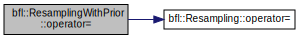
\includegraphics[width=350pt]{classbfl_1_1ResamplingWithPrior_a79ed56028dc2f97f0fb400a481998010_cgraph}
\end{center}
\end{figure}
\mbox{\Hypertarget{classbfl_1_1ResamplingWithPrior_a440090305ac024e1f5ad06fd36cccd34}\label{classbfl_1_1ResamplingWithPrior_a440090305ac024e1f5ad06fd36cccd34}} 
\index{bfl\+::\+Resampling\+With\+Prior@{bfl\+::\+Resampling\+With\+Prior}!resample@{resample}}
\index{resample@{resample}!bfl\+::\+Resampling\+With\+Prior@{bfl\+::\+Resampling\+With\+Prior}}
\subsubsection{\texorpdfstring{resample()}{resample()}}
{\footnotesize\ttfamily void Resampling\+With\+Prior\+::resample (\begin{DoxyParamCaption}\item[{const Eigen\+::\+Ref$<$ const Eigen\+::\+Matrix\+Xf $>$ \&}]{pred\+\_\+particles,  }\item[{const Eigen\+::\+Ref$<$ const Eigen\+::\+Vector\+Xf $>$ \&}]{cor\+\_\+weights,  }\item[{Eigen\+::\+Ref$<$ Eigen\+::\+Matrix\+Xf $>$}]{res\+\_\+particles,  }\item[{Eigen\+::\+Ref$<$ Eigen\+::\+Vector\+Xf $>$}]{res\+\_\+weights,  }\item[{Eigen\+::\+Ref$<$ Eigen\+::\+Vector\+Xf $>$}]{res\+\_\+parents }\end{DoxyParamCaption})\hspace{0.3cm}{\ttfamily [override]}, {\ttfamily [virtual]}}



Reimplemented from \mbox{\hyperlink{classbfl_1_1Resampling_a6b5a246250f1d193b3316c10bdc689f6}{bfl\+::\+Resampling}}.



Definition at line 53 of file Resampling\+With\+Prior.\+cpp.



References bfl\+::\+Resampling\+::resample().

Here is the call graph for this function\+:
\nopagebreak
\begin{figure}[H]
\begin{center}
\leavevmode
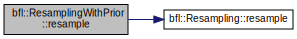
\includegraphics[width=350pt]{classbfl_1_1ResamplingWithPrior_a440090305ac024e1f5ad06fd36cccd34_cgraph}
\end{center}
\end{figure}
\mbox{\Hypertarget{classbfl_1_1ResamplingWithPrior_a9b96b3b950fccbabc6964a0443bc1a1c}\label{classbfl_1_1ResamplingWithPrior_a9b96b3b950fccbabc6964a0443bc1a1c}} 
\index{bfl\+::\+Resampling\+With\+Prior@{bfl\+::\+Resampling\+With\+Prior}!sort\+\_\+indices@{sort\+\_\+indices}}
\index{sort\+\_\+indices@{sort\+\_\+indices}!bfl\+::\+Resampling\+With\+Prior@{bfl\+::\+Resampling\+With\+Prior}}
\subsubsection{\texorpdfstring{sort\+\_\+indices()}{sort\_indices()}}
{\footnotesize\ttfamily std\+::vector$<$ unsigned int $>$ Resampling\+With\+Prior\+::sort\+\_\+indices (\begin{DoxyParamCaption}\item[{const Eigen\+::\+Ref$<$ const Eigen\+::\+Vector\+Xf $>$ \&}]{vector }\end{DoxyParamCaption})\hspace{0.3cm}{\ttfamily [private]}}



Definition at line 87 of file Resampling\+With\+Prior.\+cpp.



\subsection{Member Data Documentation}
\mbox{\Hypertarget{classbfl_1_1ResamplingWithPrior_ae5902ab0af10d76ddb9c12a15db42947}\label{classbfl_1_1ResamplingWithPrior_ae5902ab0af10d76ddb9c12a15db42947}} 
\index{bfl\+::\+Resampling\+With\+Prior@{bfl\+::\+Resampling\+With\+Prior}!init\+\_\+model\+\_\+@{init\+\_\+model\+\_\+}}
\index{init\+\_\+model\+\_\+@{init\+\_\+model\+\_\+}!bfl\+::\+Resampling\+With\+Prior@{bfl\+::\+Resampling\+With\+Prior}}
\subsubsection{\texorpdfstring{init\+\_\+model\+\_\+}{init\_model\_}}
{\footnotesize\ttfamily std\+::unique\+\_\+ptr$<$\mbox{\hyperlink{classbfl_1_1Initialization}{bfl\+::\+Initialization}}$>$ bfl\+::\+Resampling\+With\+Prior\+::init\+\_\+model\+\_\+\hspace{0.3cm}{\ttfamily [protected]}}



Definition at line 36 of file Resampling\+With\+Prior.\+h.

\mbox{\Hypertarget{classbfl_1_1ResamplingWithPrior_a5f2d0d6f948348428a992232de091c66}\label{classbfl_1_1ResamplingWithPrior_a5f2d0d6f948348428a992232de091c66}} 
\index{bfl\+::\+Resampling\+With\+Prior@{bfl\+::\+Resampling\+With\+Prior}!prior\+\_\+ratio\+\_\+@{prior\+\_\+ratio\+\_\+}}
\index{prior\+\_\+ratio\+\_\+@{prior\+\_\+ratio\+\_\+}!bfl\+::\+Resampling\+With\+Prior@{bfl\+::\+Resampling\+With\+Prior}}
\subsubsection{\texorpdfstring{prior\+\_\+ratio\+\_\+}{prior\_ratio\_}}
{\footnotesize\ttfamily double bfl\+::\+Resampling\+With\+Prior\+::prior\+\_\+ratio\+\_\+ = 0.\+5\hspace{0.3cm}{\ttfamily [protected]}}



Definition at line 38 of file Resampling\+With\+Prior.\+h.



The documentation for this class was generated from the following files\+:\begin{DoxyCompactItemize}
\item 
C\+:/\+Users/cfantacci/\+Git\+Hub/bayes-\/filters-\/lib/src/\+Bayes\+Filters/include/\+Bayes\+Filters/\mbox{\hyperlink{ResamplingWithPrior_8h}{Resampling\+With\+Prior.\+h}}\item 
C\+:/\+Users/cfantacci/\+Git\+Hub/bayes-\/filters-\/lib/src/\+Bayes\+Filters/src/\mbox{\hyperlink{ResamplingWithPrior_8cpp}{Resampling\+With\+Prior.\+cpp}}\end{DoxyCompactItemize}

\hypertarget{classbfl_1_1SIS}{}\section{bfl\+:\+:S\+IS Class Reference}
\label{classbfl_1_1SIS}\index{bfl\+::\+S\+IS@{bfl\+::\+S\+IS}}


{\ttfamily \#include $<$S\+I\+S.\+h$>$}



Inheritance diagram for bfl\+:\+:S\+IS\+:
\nopagebreak
\begin{figure}[H]
\begin{center}
\leavevmode
\includegraphics[width=188pt]{classbfl_1_1SIS__inherit__graph}
\end{center}
\end{figure}
\subsection*{Public Member Functions}
\begin{DoxyCompactItemize}
\item 
\mbox{\hyperlink{classbfl_1_1SIS_a65cd523b660bd8f41e112841aaf45c0d}{S\+IS}} () noexcept
\item 
\mbox{\hyperlink{classbfl_1_1SIS_af66e323d22b28f497152f2e3a65290ff}{S\+IS}} (\mbox{\hyperlink{classbfl_1_1SIS}{S\+IS}} \&\&sir\+\_\+pf) noexcept
\item 
virtual \mbox{\hyperlink{classbfl_1_1SIS_afe51d2eb915e0813ee4dc804a680566b}{$\sim$\+S\+IS}} () noexcept
\item 
\mbox{\hyperlink{classbfl_1_1SIS}{S\+IS}} \& \mbox{\hyperlink{classbfl_1_1SIS_a32458a24446df8126ace63f21de2bf02}{operator=}} (\mbox{\hyperlink{classbfl_1_1SIS}{S\+IS}} \&\&sir\+\_\+pf) noexcept
\item 
void \mbox{\hyperlink{classbfl_1_1SIS_aaf9f4a14d51804eddcd93aa8a5ccbba8}{initialization}} () override
\item 
void \mbox{\hyperlink{classbfl_1_1SIS_a582f06cc5456d2cc6ed8f90087cbbb4c}{filtering\+Step}} () override
\item 
void \mbox{\hyperlink{classbfl_1_1SIS_a059da4c932379643ff7005fe4d0fda89}{get\+Result}} () override
\item 
bool \mbox{\hyperlink{classbfl_1_1SIS_afb7cff1f7dae80e0e4ca84c925ca3ac3}{run\+Condition}} () override
\item 
void \mbox{\hyperlink{classbfl_1_1ParticleFilter_abfeb75fd575802f362039c26169eed8b}{set\+Initialization}} (std\+::unique\+\_\+ptr$<$ \mbox{\hyperlink{classbfl_1_1Initialization}{Initialization}} $>$ prediction)
\item 
void \mbox{\hyperlink{classbfl_1_1ParticleFilter_a213811368143c1f498c87be70cf02379}{set\+Prediction}} (std\+::unique\+\_\+ptr$<$ \mbox{\hyperlink{classbfl_1_1PFPrediction}{P\+F\+Prediction}} $>$ prediction)
\item 
void \mbox{\hyperlink{classbfl_1_1ParticleFilter_a3d2935addf4481325a3fe8b99fe4d07a}{set\+Correction}} (std\+::unique\+\_\+ptr$<$ \mbox{\hyperlink{classbfl_1_1PFCorrection}{P\+F\+Correction}} $>$ correction)
\item 
void \mbox{\hyperlink{classbfl_1_1ParticleFilter_ad1618ed06b6e6e143e309e2267b970ee}{set\+Resampling}} (std\+::unique\+\_\+ptr$<$ \mbox{\hyperlink{classbfl_1_1Resampling}{Resampling}} $>$ resampling)
\item 
virtual bool \mbox{\hyperlink{classbfl_1_1ParticleFilter_a2d7a5e7aaad179037273d35be229056d}{skip}} (const std\+::string \&what\+\_\+step, const bool status) override
\item 
bool \mbox{\hyperlink{classbfl_1_1FilteringAlgorithm_a96651f8464190c0a56d79219a1017147}{boot}} ()
\item 
void \mbox{\hyperlink{classbfl_1_1FilteringAlgorithm_a009cbe5f4bbb16967f6c6ddcaed8fbb1}{run}} ()
\item 
bool \mbox{\hyperlink{classbfl_1_1FilteringAlgorithm_a40372c24fa050eb0274371172df0a244}{wait}} ()
\item 
void \mbox{\hyperlink{classbfl_1_1FilteringAlgorithm_a2403c62fbd7bd7f5cda56a84f5f30331}{reset}} ()
\item 
void \mbox{\hyperlink{classbfl_1_1FilteringAlgorithm_a6022859aa985474fb997343cc935b11e}{reboot}} ()
\item 
bool \mbox{\hyperlink{classbfl_1_1FilteringAlgorithm_a1dc912d89ee8f96d4f3e8209865c5308}{teardown}} ()
\item 
unsigned int \mbox{\hyperlink{classbfl_1_1FilteringAlgorithm_a8c43b1f3dac30934c0a03de348d4a29d}{get\+Filtering\+Step}} ()
\item 
bool \mbox{\hyperlink{classbfl_1_1FilteringAlgorithm_a5cfecab2c778620e2557237472bb1721}{is\+Running}} ()
\end{DoxyCompactItemize}
\subsection*{Protected Attributes}
\begin{DoxyCompactItemize}
\item 
int \mbox{\hyperlink{classbfl_1_1SIS_a37062438b43e40eeaa631d17052e6c15}{simulation\+\_\+time\+\_\+}}
\item 
int \mbox{\hyperlink{classbfl_1_1SIS_a7daac4c6a2e6412d8498fda361074740}{num\+\_\+particle\+\_\+}}
\item 
int \mbox{\hyperlink{classbfl_1_1SIS_a162ac45707d6039272c1aa7b4827f274}{surv\+\_\+x\+\_\+}}
\item 
int \mbox{\hyperlink{classbfl_1_1SIS_af39569c2ba7035387556e8a31ca633e8}{surv\+\_\+y\+\_\+}}
\item 
Eigen\+::\+Matrix\+Xf \mbox{\hyperlink{classbfl_1_1SIS_a05ad3f95a4402f875aa2cf98c20f0ac6}{object\+\_\+}}
\item 
Eigen\+::\+Matrix\+Xf \mbox{\hyperlink{classbfl_1_1SIS_aed940f18871c4b12b70bf720bc671184}{measurement\+\_\+}}
\item 
Eigen\+::\+Matrix\+Xf \mbox{\hyperlink{classbfl_1_1SIS_a489ce9127eff33afdecab341774662dd}{pred\+\_\+particle\+\_\+}}
\item 
Eigen\+::\+Vector\+Xf \mbox{\hyperlink{classbfl_1_1SIS_a736b0b1a524f96273201f82d153f55d2}{pred\+\_\+weight\+\_\+}}
\item 
Eigen\+::\+Matrix\+Xf \mbox{\hyperlink{classbfl_1_1SIS_aa4d63e8986156c13cc721c9c94c983d6}{cor\+\_\+particle\+\_\+}}
\item 
Eigen\+::\+Vector\+Xf \mbox{\hyperlink{classbfl_1_1SIS_a3e39c33d92371409b992fb4b856d48c0}{cor\+\_\+weight\+\_\+}}
\item 
std\+::vector$<$ Eigen\+::\+Matrix\+Xf $>$ \mbox{\hyperlink{classbfl_1_1SIS_a153d27bbf73332c052085d286455e435}{result\+\_\+pred\+\_\+particle\+\_\+}}
\item 
std\+::vector$<$ Eigen\+::\+Vector\+Xf $>$ \mbox{\hyperlink{classbfl_1_1SIS_a9af5a5fc5ee16acb826093a1acc7330d}{result\+\_\+pred\+\_\+weight\+\_\+}}
\item 
std\+::vector$<$ Eigen\+::\+Matrix\+Xf $>$ \mbox{\hyperlink{classbfl_1_1SIS_ad1a6248ef476eac5f624780676e96a15}{result\+\_\+cor\+\_\+particle\+\_\+}}
\item 
std\+::vector$<$ Eigen\+::\+Vector\+Xf $>$ \mbox{\hyperlink{classbfl_1_1SIS_a41ae49a78766ccbb0356ff2cdc2fe7ee}{result\+\_\+cor\+\_\+weight\+\_\+}}
\item 
std\+::unique\+\_\+ptr$<$ \mbox{\hyperlink{classbfl_1_1Initialization}{Initialization}} $>$ \mbox{\hyperlink{classbfl_1_1ParticleFilter_a5aff690b4287811912a62548188a0dda}{initialization\+\_\+}}
\item 
std\+::unique\+\_\+ptr$<$ \mbox{\hyperlink{classbfl_1_1PFPrediction}{P\+F\+Prediction}} $>$ \mbox{\hyperlink{classbfl_1_1ParticleFilter_ab86f707d29a823423fe35de37e8f9d8e}{prediction\+\_\+}}
\item 
std\+::unique\+\_\+ptr$<$ \mbox{\hyperlink{classbfl_1_1PFCorrection}{P\+F\+Correction}} $>$ \mbox{\hyperlink{classbfl_1_1ParticleFilter_a691428357c812ba009e995175778c173}{correction\+\_\+}}
\item 
std\+::unique\+\_\+ptr$<$ \mbox{\hyperlink{classbfl_1_1Resampling}{Resampling}} $>$ \mbox{\hyperlink{classbfl_1_1ParticleFilter_a9b0b855942fa4fb847443b10fe26c589}{resampling\+\_\+}}
\end{DoxyCompactItemize}


\subsection{Detailed Description}


Definition at line 18 of file S\+I\+S.\+h.



\subsection{Constructor \& Destructor Documentation}
\mbox{\Hypertarget{classbfl_1_1SIS_a65cd523b660bd8f41e112841aaf45c0d}\label{classbfl_1_1SIS_a65cd523b660bd8f41e112841aaf45c0d}} 
\index{bfl\+::\+S\+IS@{bfl\+::\+S\+IS}!S\+IS@{S\+IS}}
\index{S\+IS@{S\+IS}!bfl\+::\+S\+IS@{bfl\+::\+S\+IS}}
\subsubsection{\texorpdfstring{S\+I\+S()}{SIS()}\hspace{0.1cm}{\footnotesize\ttfamily [1/2]}}
{\footnotesize\ttfamily S\+I\+S\+::\+S\+IS (\begin{DoxyParamCaption}{ }\end{DoxyParamCaption})\hspace{0.3cm}{\ttfamily [noexcept]}}



Definition at line 13 of file S\+I\+S.\+cpp.

\mbox{\Hypertarget{classbfl_1_1SIS_af66e323d22b28f497152f2e3a65290ff}\label{classbfl_1_1SIS_af66e323d22b28f497152f2e3a65290ff}} 
\index{bfl\+::\+S\+IS@{bfl\+::\+S\+IS}!S\+IS@{S\+IS}}
\index{S\+IS@{S\+IS}!bfl\+::\+S\+IS@{bfl\+::\+S\+IS}}
\subsubsection{\texorpdfstring{S\+I\+S()}{SIS()}\hspace{0.1cm}{\footnotesize\ttfamily [2/2]}}
{\footnotesize\ttfamily S\+I\+S\+::\+S\+IS (\begin{DoxyParamCaption}\item[{\mbox{\hyperlink{classbfl_1_1SIS}{S\+IS}} \&\&}]{sir\+\_\+pf }\end{DoxyParamCaption})\hspace{0.3cm}{\ttfamily [noexcept]}}



Definition at line 19 of file S\+I\+S.\+cpp.

\mbox{\Hypertarget{classbfl_1_1SIS_afe51d2eb915e0813ee4dc804a680566b}\label{classbfl_1_1SIS_afe51d2eb915e0813ee4dc804a680566b}} 
\index{bfl\+::\+S\+IS@{bfl\+::\+S\+IS}!````~S\+IS@{$\sim$\+S\+IS}}
\index{````~S\+IS@{$\sim$\+S\+IS}!bfl\+::\+S\+IS@{bfl\+::\+S\+IS}}
\subsubsection{\texorpdfstring{$\sim$\+S\+I\+S()}{~SIS()}}
{\footnotesize\ttfamily S\+I\+S\+::$\sim$\+S\+IS (\begin{DoxyParamCaption}{ }\end{DoxyParamCaption})\hspace{0.3cm}{\ttfamily [virtual]}, {\ttfamily [noexcept]}}



Definition at line 16 of file S\+I\+S.\+cpp.



\subsection{Member Function Documentation}
\mbox{\Hypertarget{classbfl_1_1FilteringAlgorithm_a96651f8464190c0a56d79219a1017147}\label{classbfl_1_1FilteringAlgorithm_a96651f8464190c0a56d79219a1017147}} 
\index{bfl\+::\+S\+IS@{bfl\+::\+S\+IS}!boot@{boot}}
\index{boot@{boot}!bfl\+::\+S\+IS@{bfl\+::\+S\+IS}}
\subsubsection{\texorpdfstring{boot()}{boot()}}
{\footnotesize\ttfamily bool Filtering\+Algorithm\+::boot (\begin{DoxyParamCaption}{ }\end{DoxyParamCaption})\hspace{0.3cm}{\ttfamily [inherited]}}



Definition at line 8 of file Filtering\+Algorithm.\+cpp.



References bfl\+::\+Filtering\+Algorithm\+::filtering\+\_\+thread\+\_\+, and bfl\+::\+Filtering\+Algorithm\+::filtering\+Recursion().

Here is the call graph for this function\+:
\nopagebreak
\begin{figure}[H]
\begin{center}
\leavevmode
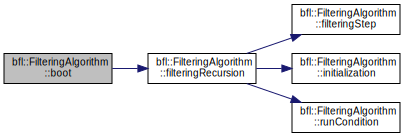
\includegraphics[width=350pt]{classbfl_1_1FilteringAlgorithm_a96651f8464190c0a56d79219a1017147_cgraph}
\end{center}
\end{figure}
\mbox{\Hypertarget{classbfl_1_1SIS_a582f06cc5456d2cc6ed8f90087cbbb4c}\label{classbfl_1_1SIS_a582f06cc5456d2cc6ed8f90087cbbb4c}} 
\index{bfl\+::\+S\+IS@{bfl\+::\+S\+IS}!filtering\+Step@{filtering\+Step}}
\index{filtering\+Step@{filtering\+Step}!bfl\+::\+S\+IS@{bfl\+::\+S\+IS}}
\subsubsection{\texorpdfstring{filtering\+Step()}{filteringStep()}}
{\footnotesize\ttfamily void S\+I\+S\+::filtering\+Step (\begin{DoxyParamCaption}{ }\end{DoxyParamCaption})\hspace{0.3cm}{\ttfamily [override]}, {\ttfamily [virtual]}}



Implements \mbox{\hyperlink{classbfl_1_1FilteringAlgorithm_ab3bceb43b5810a4bf1da884b8a0b145a}{bfl\+::\+Filtering\+Algorithm}}.



Definition at line 73 of file S\+I\+S.\+cpp.

\mbox{\Hypertarget{classbfl_1_1FilteringAlgorithm_a8c43b1f3dac30934c0a03de348d4a29d}\label{classbfl_1_1FilteringAlgorithm_a8c43b1f3dac30934c0a03de348d4a29d}} 
\index{bfl\+::\+S\+IS@{bfl\+::\+S\+IS}!get\+Filtering\+Step@{get\+Filtering\+Step}}
\index{get\+Filtering\+Step@{get\+Filtering\+Step}!bfl\+::\+S\+IS@{bfl\+::\+S\+IS}}
\subsubsection{\texorpdfstring{get\+Filtering\+Step()}{getFilteringStep()}}
{\footnotesize\ttfamily unsigned int Filtering\+Algorithm\+::get\+Filtering\+Step (\begin{DoxyParamCaption}{ }\end{DoxyParamCaption})\hspace{0.3cm}{\ttfamily [inherited]}}



Definition at line 86 of file Filtering\+Algorithm.\+cpp.



References bfl\+::\+Filtering\+Algorithm\+::filtering\+\_\+step\+\_\+.

\mbox{\Hypertarget{classbfl_1_1SIS_a059da4c932379643ff7005fe4d0fda89}\label{classbfl_1_1SIS_a059da4c932379643ff7005fe4d0fda89}} 
\index{bfl\+::\+S\+IS@{bfl\+::\+S\+IS}!get\+Result@{get\+Result}}
\index{get\+Result@{get\+Result}!bfl\+::\+S\+IS@{bfl\+::\+S\+IS}}
\subsubsection{\texorpdfstring{get\+Result()}{getResult()}}
{\footnotesize\ttfamily void S\+I\+S\+::get\+Result (\begin{DoxyParamCaption}{ }\end{DoxyParamCaption})\hspace{0.3cm}{\ttfamily [override]}, {\ttfamily [virtual]}}



Implements \mbox{\hyperlink{classbfl_1_1FilteringAlgorithm_acdfebf68405a427491e4dd9d020ae09b}{bfl\+::\+Filtering\+Algorithm}}.



Definition at line 111 of file S\+I\+S.\+cpp.

\mbox{\Hypertarget{classbfl_1_1SIS_aaf9f4a14d51804eddcd93aa8a5ccbba8}\label{classbfl_1_1SIS_aaf9f4a14d51804eddcd93aa8a5ccbba8}} 
\index{bfl\+::\+S\+IS@{bfl\+::\+S\+IS}!initialization@{initialization}}
\index{initialization@{initialization}!bfl\+::\+S\+IS@{bfl\+::\+S\+IS}}
\subsubsection{\texorpdfstring{initialization()}{initialization()}}
{\footnotesize\ttfamily void S\+I\+S\+::initialization (\begin{DoxyParamCaption}{ }\end{DoxyParamCaption})\hspace{0.3cm}{\ttfamily [override]}, {\ttfamily [virtual]}}



Implements \mbox{\hyperlink{classbfl_1_1FilteringAlgorithm_af2a072aa51407fe5544bdbb7ce466e2a}{bfl\+::\+Filtering\+Algorithm}}.



Definition at line 31 of file S\+I\+S.\+cpp.

\mbox{\Hypertarget{classbfl_1_1FilteringAlgorithm_a5cfecab2c778620e2557237472bb1721}\label{classbfl_1_1FilteringAlgorithm_a5cfecab2c778620e2557237472bb1721}} 
\index{bfl\+::\+S\+IS@{bfl\+::\+S\+IS}!is\+Running@{is\+Running}}
\index{is\+Running@{is\+Running}!bfl\+::\+S\+IS@{bfl\+::\+S\+IS}}
\subsubsection{\texorpdfstring{is\+Running()}{isRunning()}}
{\footnotesize\ttfamily bool Filtering\+Algorithm\+::is\+Running (\begin{DoxyParamCaption}{ }\end{DoxyParamCaption})\hspace{0.3cm}{\ttfamily [inherited]}}



Definition at line 92 of file Filtering\+Algorithm.\+cpp.



References bfl\+::\+Filtering\+Algorithm\+::run\+\_\+.

\mbox{\Hypertarget{classbfl_1_1SIS_a32458a24446df8126ace63f21de2bf02}\label{classbfl_1_1SIS_a32458a24446df8126ace63f21de2bf02}} 
\index{bfl\+::\+S\+IS@{bfl\+::\+S\+IS}!operator=@{operator=}}
\index{operator=@{operator=}!bfl\+::\+S\+IS@{bfl\+::\+S\+IS}}
\subsubsection{\texorpdfstring{operator=()}{operator=()}}
{\footnotesize\ttfamily \mbox{\hyperlink{classbfl_1_1SIS}{S\+IS}} \& S\+I\+S\+::operator= (\begin{DoxyParamCaption}\item[{\mbox{\hyperlink{classbfl_1_1SIS}{S\+IS}} \&\&}]{sir\+\_\+pf }\end{DoxyParamCaption})\hspace{0.3cm}{\ttfamily [noexcept]}}



Definition at line 23 of file S\+I\+S.\+cpp.



References bfl\+::\+Particle\+Filter\+::operator=().

Here is the call graph for this function\+:
\nopagebreak
\begin{figure}[H]
\begin{center}
\leavevmode
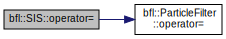
\includegraphics[width=298pt]{classbfl_1_1SIS_a32458a24446df8126ace63f21de2bf02_cgraph}
\end{center}
\end{figure}
\mbox{\Hypertarget{classbfl_1_1FilteringAlgorithm_a6022859aa985474fb997343cc935b11e}\label{classbfl_1_1FilteringAlgorithm_a6022859aa985474fb997343cc935b11e}} 
\index{bfl\+::\+S\+IS@{bfl\+::\+S\+IS}!reboot@{reboot}}
\index{reboot@{reboot}!bfl\+::\+S\+IS@{bfl\+::\+S\+IS}}
\subsubsection{\texorpdfstring{reboot()}{reboot()}}
{\footnotesize\ttfamily void Filtering\+Algorithm\+::reboot (\begin{DoxyParamCaption}{ }\end{DoxyParamCaption})\hspace{0.3cm}{\ttfamily [inherited]}}



Definition at line 66 of file Filtering\+Algorithm.\+cpp.



References bfl\+::\+Filtering\+Algorithm\+::cv\+\_\+run\+\_\+, bfl\+::\+Filtering\+Algorithm\+::mtx\+\_\+run\+\_\+, bfl\+::\+Filtering\+Algorithm\+::reset\+\_\+, and bfl\+::\+Filtering\+Algorithm\+::run\+\_\+.

\mbox{\Hypertarget{classbfl_1_1FilteringAlgorithm_a2403c62fbd7bd7f5cda56a84f5f30331}\label{classbfl_1_1FilteringAlgorithm_a2403c62fbd7bd7f5cda56a84f5f30331}} 
\index{bfl\+::\+S\+IS@{bfl\+::\+S\+IS}!reset@{reset}}
\index{reset@{reset}!bfl\+::\+S\+IS@{bfl\+::\+S\+IS}}
\subsubsection{\texorpdfstring{reset()}{reset()}}
{\footnotesize\ttfamily void Filtering\+Algorithm\+::reset (\begin{DoxyParamCaption}{ }\end{DoxyParamCaption})\hspace{0.3cm}{\ttfamily [inherited]}}



Definition at line 60 of file Filtering\+Algorithm.\+cpp.



References bfl\+::\+Filtering\+Algorithm\+::reset\+\_\+.

\mbox{\Hypertarget{classbfl_1_1FilteringAlgorithm_a009cbe5f4bbb16967f6c6ddcaed8fbb1}\label{classbfl_1_1FilteringAlgorithm_a009cbe5f4bbb16967f6c6ddcaed8fbb1}} 
\index{bfl\+::\+S\+IS@{bfl\+::\+S\+IS}!run@{run}}
\index{run@{run}!bfl\+::\+S\+IS@{bfl\+::\+S\+IS}}
\subsubsection{\texorpdfstring{run()}{run()}}
{\footnotesize\ttfamily void Filtering\+Algorithm\+::run (\begin{DoxyParamCaption}{ }\end{DoxyParamCaption})\hspace{0.3cm}{\ttfamily [inherited]}}



Definition at line 26 of file Filtering\+Algorithm.\+cpp.



References bfl\+::\+Filtering\+Algorithm\+::cv\+\_\+run\+\_\+, bfl\+::\+Filtering\+Algorithm\+::mtx\+\_\+run\+\_\+, and bfl\+::\+Filtering\+Algorithm\+::run\+\_\+.

\mbox{\Hypertarget{classbfl_1_1SIS_afb7cff1f7dae80e0e4ca84c925ca3ac3}\label{classbfl_1_1SIS_afb7cff1f7dae80e0e4ca84c925ca3ac3}} 
\index{bfl\+::\+S\+IS@{bfl\+::\+S\+IS}!run\+Condition@{run\+Condition}}
\index{run\+Condition@{run\+Condition}!bfl\+::\+S\+IS@{bfl\+::\+S\+IS}}
\subsubsection{\texorpdfstring{run\+Condition()}{runCondition()}}
{\footnotesize\ttfamily bool bfl\+::\+S\+I\+S\+::run\+Condition (\begin{DoxyParamCaption}{ }\end{DoxyParamCaption})\hspace{0.3cm}{\ttfamily [inline]}, {\ttfamily [override]}, {\ttfamily [virtual]}}



Implements \mbox{\hyperlink{classbfl_1_1FilteringAlgorithm_a5fc12882356f6906b102fbfff2bc4b7c}{bfl\+::\+Filtering\+Algorithm}}.



Definition at line 35 of file S\+I\+S.\+h.

\mbox{\Hypertarget{classbfl_1_1ParticleFilter_a3d2935addf4481325a3fe8b99fe4d07a}\label{classbfl_1_1ParticleFilter_a3d2935addf4481325a3fe8b99fe4d07a}} 
\index{bfl\+::\+S\+IS@{bfl\+::\+S\+IS}!set\+Correction@{set\+Correction}}
\index{set\+Correction@{set\+Correction}!bfl\+::\+S\+IS@{bfl\+::\+S\+IS}}
\subsubsection{\texorpdfstring{set\+Correction()}{setCorrection()}}
{\footnotesize\ttfamily void Particle\+Filter\+::set\+Correction (\begin{DoxyParamCaption}\item[{std\+::unique\+\_\+ptr$<$ \mbox{\hyperlink{classbfl_1_1PFCorrection}{P\+F\+Correction}} $>$}]{correction }\end{DoxyParamCaption})\hspace{0.3cm}{\ttfamily [inherited]}}



Definition at line 42 of file Particle\+Filter.\+cpp.



References bfl\+::\+Particle\+Filter\+::correction\+\_\+.

\mbox{\Hypertarget{classbfl_1_1ParticleFilter_abfeb75fd575802f362039c26169eed8b}\label{classbfl_1_1ParticleFilter_abfeb75fd575802f362039c26169eed8b}} 
\index{bfl\+::\+S\+IS@{bfl\+::\+S\+IS}!set\+Initialization@{set\+Initialization}}
\index{set\+Initialization@{set\+Initialization}!bfl\+::\+S\+IS@{bfl\+::\+S\+IS}}
\subsubsection{\texorpdfstring{set\+Initialization()}{setInitialization()}}
{\footnotesize\ttfamily void Particle\+Filter\+::set\+Initialization (\begin{DoxyParamCaption}\item[{std\+::unique\+\_\+ptr$<$ \mbox{\hyperlink{classbfl_1_1Initialization}{Initialization}} $>$}]{prediction }\end{DoxyParamCaption})\hspace{0.3cm}{\ttfamily [inherited]}}



Definition at line 30 of file Particle\+Filter.\+cpp.



References bfl\+::\+Filtering\+Algorithm\+::initialization(), and bfl\+::\+Particle\+Filter\+::initialization\+\_\+.

Here is the call graph for this function\+:
\nopagebreak
\begin{figure}[H]
\begin{center}
\leavevmode
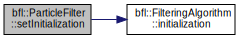
\includegraphics[width=311pt]{classbfl_1_1ParticleFilter_abfeb75fd575802f362039c26169eed8b_cgraph}
\end{center}
\end{figure}
\mbox{\Hypertarget{classbfl_1_1ParticleFilter_a213811368143c1f498c87be70cf02379}\label{classbfl_1_1ParticleFilter_a213811368143c1f498c87be70cf02379}} 
\index{bfl\+::\+S\+IS@{bfl\+::\+S\+IS}!set\+Prediction@{set\+Prediction}}
\index{set\+Prediction@{set\+Prediction}!bfl\+::\+S\+IS@{bfl\+::\+S\+IS}}
\subsubsection{\texorpdfstring{set\+Prediction()}{setPrediction()}}
{\footnotesize\ttfamily void Particle\+Filter\+::set\+Prediction (\begin{DoxyParamCaption}\item[{std\+::unique\+\_\+ptr$<$ \mbox{\hyperlink{classbfl_1_1PFPrediction}{P\+F\+Prediction}} $>$}]{prediction }\end{DoxyParamCaption})\hspace{0.3cm}{\ttfamily [inherited]}}



Definition at line 36 of file Particle\+Filter.\+cpp.



References bfl\+::\+Particle\+Filter\+::prediction\+\_\+.

\mbox{\Hypertarget{classbfl_1_1ParticleFilter_ad1618ed06b6e6e143e309e2267b970ee}\label{classbfl_1_1ParticleFilter_ad1618ed06b6e6e143e309e2267b970ee}} 
\index{bfl\+::\+S\+IS@{bfl\+::\+S\+IS}!set\+Resampling@{set\+Resampling}}
\index{set\+Resampling@{set\+Resampling}!bfl\+::\+S\+IS@{bfl\+::\+S\+IS}}
\subsubsection{\texorpdfstring{set\+Resampling()}{setResampling()}}
{\footnotesize\ttfamily void Particle\+Filter\+::set\+Resampling (\begin{DoxyParamCaption}\item[{std\+::unique\+\_\+ptr$<$ \mbox{\hyperlink{classbfl_1_1Resampling}{Resampling}} $>$}]{resampling }\end{DoxyParamCaption})\hspace{0.3cm}{\ttfamily [inherited]}}



Definition at line 48 of file Particle\+Filter.\+cpp.



References bfl\+::\+Particle\+Filter\+::resampling\+\_\+.

\mbox{\Hypertarget{classbfl_1_1ParticleFilter_a2d7a5e7aaad179037273d35be229056d}\label{classbfl_1_1ParticleFilter_a2d7a5e7aaad179037273d35be229056d}} 
\index{bfl\+::\+S\+IS@{bfl\+::\+S\+IS}!skip@{skip}}
\index{skip@{skip}!bfl\+::\+S\+IS@{bfl\+::\+S\+IS}}
\subsubsection{\texorpdfstring{skip()}{skip()}}
{\footnotesize\ttfamily bool Particle\+Filter\+::skip (\begin{DoxyParamCaption}\item[{const std\+::string \&}]{what\+\_\+step,  }\item[{const bool}]{status }\end{DoxyParamCaption})\hspace{0.3cm}{\ttfamily [override]}, {\ttfamily [virtual]}, {\ttfamily [inherited]}}



Implements \mbox{\hyperlink{classbfl_1_1FilteringAlgorithm_ac8a718a614905d89d6a43bbbc70d68b2}{bfl\+::\+Filtering\+Algorithm}}.



Definition at line 54 of file Particle\+Filter.\+cpp.



References bfl\+::\+Particle\+Filter\+::correction\+\_\+, and bfl\+::\+Particle\+Filter\+::prediction\+\_\+.

\mbox{\Hypertarget{classbfl_1_1FilteringAlgorithm_a1dc912d89ee8f96d4f3e8209865c5308}\label{classbfl_1_1FilteringAlgorithm_a1dc912d89ee8f96d4f3e8209865c5308}} 
\index{bfl\+::\+S\+IS@{bfl\+::\+S\+IS}!teardown@{teardown}}
\index{teardown@{teardown}!bfl\+::\+S\+IS@{bfl\+::\+S\+IS}}
\subsubsection{\texorpdfstring{teardown()}{teardown()}}
{\footnotesize\ttfamily bool Filtering\+Algorithm\+::teardown (\begin{DoxyParamCaption}{ }\end{DoxyParamCaption})\hspace{0.3cm}{\ttfamily [inherited]}}



Definition at line 75 of file Filtering\+Algorithm.\+cpp.



References bfl\+::\+Filtering\+Algorithm\+::teardown\+\_\+.

\mbox{\Hypertarget{classbfl_1_1FilteringAlgorithm_a40372c24fa050eb0274371172df0a244}\label{classbfl_1_1FilteringAlgorithm_a40372c24fa050eb0274371172df0a244}} 
\index{bfl\+::\+S\+IS@{bfl\+::\+S\+IS}!wait@{wait}}
\index{wait@{wait}!bfl\+::\+S\+IS@{bfl\+::\+S\+IS}}
\subsubsection{\texorpdfstring{wait()}{wait()}}
{\footnotesize\ttfamily bool Filtering\+Algorithm\+::wait (\begin{DoxyParamCaption}{ }\end{DoxyParamCaption})\hspace{0.3cm}{\ttfamily [inherited]}}



Definition at line 34 of file Filtering\+Algorithm.\+cpp.



References bfl\+::\+Filtering\+Algorithm\+::filtering\+\_\+thread\+\_\+.



\subsection{Member Data Documentation}
\mbox{\Hypertarget{classbfl_1_1SIS_aa4d63e8986156c13cc721c9c94c983d6}\label{classbfl_1_1SIS_aa4d63e8986156c13cc721c9c94c983d6}} 
\index{bfl\+::\+S\+IS@{bfl\+::\+S\+IS}!cor\+\_\+particle\+\_\+@{cor\+\_\+particle\+\_\+}}
\index{cor\+\_\+particle\+\_\+@{cor\+\_\+particle\+\_\+}!bfl\+::\+S\+IS@{bfl\+::\+S\+IS}}
\subsubsection{\texorpdfstring{cor\+\_\+particle\+\_\+}{cor\_particle\_}}
{\footnotesize\ttfamily Eigen\+::\+Matrix\+Xf bfl\+::\+S\+I\+S\+::cor\+\_\+particle\+\_\+\hspace{0.3cm}{\ttfamily [protected]}}



Definition at line 49 of file S\+I\+S.\+h.

\mbox{\Hypertarget{classbfl_1_1SIS_a3e39c33d92371409b992fb4b856d48c0}\label{classbfl_1_1SIS_a3e39c33d92371409b992fb4b856d48c0}} 
\index{bfl\+::\+S\+IS@{bfl\+::\+S\+IS}!cor\+\_\+weight\+\_\+@{cor\+\_\+weight\+\_\+}}
\index{cor\+\_\+weight\+\_\+@{cor\+\_\+weight\+\_\+}!bfl\+::\+S\+IS@{bfl\+::\+S\+IS}}
\subsubsection{\texorpdfstring{cor\+\_\+weight\+\_\+}{cor\_weight\_}}
{\footnotesize\ttfamily Eigen\+::\+Vector\+Xf bfl\+::\+S\+I\+S\+::cor\+\_\+weight\+\_\+\hspace{0.3cm}{\ttfamily [protected]}}



Definition at line 50 of file S\+I\+S.\+h.

\mbox{\Hypertarget{classbfl_1_1ParticleFilter_a691428357c812ba009e995175778c173}\label{classbfl_1_1ParticleFilter_a691428357c812ba009e995175778c173}} 
\index{bfl\+::\+S\+IS@{bfl\+::\+S\+IS}!correction\+\_\+@{correction\+\_\+}}
\index{correction\+\_\+@{correction\+\_\+}!bfl\+::\+S\+IS@{bfl\+::\+S\+IS}}
\subsubsection{\texorpdfstring{correction\+\_\+}{correction\_}}
{\footnotesize\ttfamily std\+::unique\+\_\+ptr$<$\mbox{\hyperlink{classbfl_1_1PFCorrection}{P\+F\+Correction}}$>$ bfl\+::\+Particle\+Filter\+::correction\+\_\+\hspace{0.3cm}{\ttfamily [protected]}, {\ttfamily [inherited]}}



Definition at line 41 of file Particle\+Filter.\+h.



Referenced by bfl\+::\+Particle\+Filter\+::set\+Correction(), and bfl\+::\+Particle\+Filter\+::skip().

\mbox{\Hypertarget{classbfl_1_1ParticleFilter_a5aff690b4287811912a62548188a0dda}\label{classbfl_1_1ParticleFilter_a5aff690b4287811912a62548188a0dda}} 
\index{bfl\+::\+S\+IS@{bfl\+::\+S\+IS}!initialization\+\_\+@{initialization\+\_\+}}
\index{initialization\+\_\+@{initialization\+\_\+}!bfl\+::\+S\+IS@{bfl\+::\+S\+IS}}
\subsubsection{\texorpdfstring{initialization\+\_\+}{initialization\_}}
{\footnotesize\ttfamily std\+::unique\+\_\+ptr$<$\mbox{\hyperlink{classbfl_1_1Initialization}{Initialization}}$>$ bfl\+::\+Particle\+Filter\+::initialization\+\_\+\hspace{0.3cm}{\ttfamily [protected]}, {\ttfamily [inherited]}}



Definition at line 39 of file Particle\+Filter.\+h.



Referenced by bfl\+::\+Particle\+Filter\+::set\+Initialization().

\mbox{\Hypertarget{classbfl_1_1SIS_aed940f18871c4b12b70bf720bc671184}\label{classbfl_1_1SIS_aed940f18871c4b12b70bf720bc671184}} 
\index{bfl\+::\+S\+IS@{bfl\+::\+S\+IS}!measurement\+\_\+@{measurement\+\_\+}}
\index{measurement\+\_\+@{measurement\+\_\+}!bfl\+::\+S\+IS@{bfl\+::\+S\+IS}}
\subsubsection{\texorpdfstring{measurement\+\_\+}{measurement\_}}
{\footnotesize\ttfamily Eigen\+::\+Matrix\+Xf bfl\+::\+S\+I\+S\+::measurement\+\_\+\hspace{0.3cm}{\ttfamily [protected]}}



Definition at line 44 of file S\+I\+S.\+h.

\mbox{\Hypertarget{classbfl_1_1SIS_a7daac4c6a2e6412d8498fda361074740}\label{classbfl_1_1SIS_a7daac4c6a2e6412d8498fda361074740}} 
\index{bfl\+::\+S\+IS@{bfl\+::\+S\+IS}!num\+\_\+particle\+\_\+@{num\+\_\+particle\+\_\+}}
\index{num\+\_\+particle\+\_\+@{num\+\_\+particle\+\_\+}!bfl\+::\+S\+IS@{bfl\+::\+S\+IS}}
\subsubsection{\texorpdfstring{num\+\_\+particle\+\_\+}{num\_particle\_}}
{\footnotesize\ttfamily int bfl\+::\+S\+I\+S\+::num\+\_\+particle\+\_\+\hspace{0.3cm}{\ttfamily [protected]}}



Definition at line 39 of file S\+I\+S.\+h.

\mbox{\Hypertarget{classbfl_1_1SIS_a05ad3f95a4402f875aa2cf98c20f0ac6}\label{classbfl_1_1SIS_a05ad3f95a4402f875aa2cf98c20f0ac6}} 
\index{bfl\+::\+S\+IS@{bfl\+::\+S\+IS}!object\+\_\+@{object\+\_\+}}
\index{object\+\_\+@{object\+\_\+}!bfl\+::\+S\+IS@{bfl\+::\+S\+IS}}
\subsubsection{\texorpdfstring{object\+\_\+}{object\_}}
{\footnotesize\ttfamily Eigen\+::\+Matrix\+Xf bfl\+::\+S\+I\+S\+::object\+\_\+\hspace{0.3cm}{\ttfamily [protected]}}



Definition at line 43 of file S\+I\+S.\+h.

\mbox{\Hypertarget{classbfl_1_1SIS_a489ce9127eff33afdecab341774662dd}\label{classbfl_1_1SIS_a489ce9127eff33afdecab341774662dd}} 
\index{bfl\+::\+S\+IS@{bfl\+::\+S\+IS}!pred\+\_\+particle\+\_\+@{pred\+\_\+particle\+\_\+}}
\index{pred\+\_\+particle\+\_\+@{pred\+\_\+particle\+\_\+}!bfl\+::\+S\+IS@{bfl\+::\+S\+IS}}
\subsubsection{\texorpdfstring{pred\+\_\+particle\+\_\+}{pred\_particle\_}}
{\footnotesize\ttfamily Eigen\+::\+Matrix\+Xf bfl\+::\+S\+I\+S\+::pred\+\_\+particle\+\_\+\hspace{0.3cm}{\ttfamily [protected]}}



Definition at line 46 of file S\+I\+S.\+h.

\mbox{\Hypertarget{classbfl_1_1SIS_a736b0b1a524f96273201f82d153f55d2}\label{classbfl_1_1SIS_a736b0b1a524f96273201f82d153f55d2}} 
\index{bfl\+::\+S\+IS@{bfl\+::\+S\+IS}!pred\+\_\+weight\+\_\+@{pred\+\_\+weight\+\_\+}}
\index{pred\+\_\+weight\+\_\+@{pred\+\_\+weight\+\_\+}!bfl\+::\+S\+IS@{bfl\+::\+S\+IS}}
\subsubsection{\texorpdfstring{pred\+\_\+weight\+\_\+}{pred\_weight\_}}
{\footnotesize\ttfamily Eigen\+::\+Vector\+Xf bfl\+::\+S\+I\+S\+::pred\+\_\+weight\+\_\+\hspace{0.3cm}{\ttfamily [protected]}}



Definition at line 47 of file S\+I\+S.\+h.

\mbox{\Hypertarget{classbfl_1_1ParticleFilter_ab86f707d29a823423fe35de37e8f9d8e}\label{classbfl_1_1ParticleFilter_ab86f707d29a823423fe35de37e8f9d8e}} 
\index{bfl\+::\+S\+IS@{bfl\+::\+S\+IS}!prediction\+\_\+@{prediction\+\_\+}}
\index{prediction\+\_\+@{prediction\+\_\+}!bfl\+::\+S\+IS@{bfl\+::\+S\+IS}}
\subsubsection{\texorpdfstring{prediction\+\_\+}{prediction\_}}
{\footnotesize\ttfamily std\+::unique\+\_\+ptr$<$\mbox{\hyperlink{classbfl_1_1PFPrediction}{P\+F\+Prediction}}$>$ bfl\+::\+Particle\+Filter\+::prediction\+\_\+\hspace{0.3cm}{\ttfamily [protected]}, {\ttfamily [inherited]}}



Definition at line 40 of file Particle\+Filter.\+h.



Referenced by bfl\+::\+Particle\+Filter\+::set\+Prediction(), and bfl\+::\+Particle\+Filter\+::skip().

\mbox{\Hypertarget{classbfl_1_1ParticleFilter_a9b0b855942fa4fb847443b10fe26c589}\label{classbfl_1_1ParticleFilter_a9b0b855942fa4fb847443b10fe26c589}} 
\index{bfl\+::\+S\+IS@{bfl\+::\+S\+IS}!resampling\+\_\+@{resampling\+\_\+}}
\index{resampling\+\_\+@{resampling\+\_\+}!bfl\+::\+S\+IS@{bfl\+::\+S\+IS}}
\subsubsection{\texorpdfstring{resampling\+\_\+}{resampling\_}}
{\footnotesize\ttfamily std\+::unique\+\_\+ptr$<$\mbox{\hyperlink{classbfl_1_1Resampling}{Resampling}}$>$ bfl\+::\+Particle\+Filter\+::resampling\+\_\+\hspace{0.3cm}{\ttfamily [protected]}, {\ttfamily [inherited]}}



Definition at line 42 of file Particle\+Filter.\+h.



Referenced by bfl\+::\+Particle\+Filter\+::set\+Resampling().

\mbox{\Hypertarget{classbfl_1_1SIS_ad1a6248ef476eac5f624780676e96a15}\label{classbfl_1_1SIS_ad1a6248ef476eac5f624780676e96a15}} 
\index{bfl\+::\+S\+IS@{bfl\+::\+S\+IS}!result\+\_\+cor\+\_\+particle\+\_\+@{result\+\_\+cor\+\_\+particle\+\_\+}}
\index{result\+\_\+cor\+\_\+particle\+\_\+@{result\+\_\+cor\+\_\+particle\+\_\+}!bfl\+::\+S\+IS@{bfl\+::\+S\+IS}}
\subsubsection{\texorpdfstring{result\+\_\+cor\+\_\+particle\+\_\+}{result\_cor\_particle\_}}
{\footnotesize\ttfamily std\+::vector$<$Eigen\+::\+Matrix\+Xf$>$ bfl\+::\+S\+I\+S\+::result\+\_\+cor\+\_\+particle\+\_\+\hspace{0.3cm}{\ttfamily [protected]}}



Definition at line 55 of file S\+I\+S.\+h.

\mbox{\Hypertarget{classbfl_1_1SIS_a41ae49a78766ccbb0356ff2cdc2fe7ee}\label{classbfl_1_1SIS_a41ae49a78766ccbb0356ff2cdc2fe7ee}} 
\index{bfl\+::\+S\+IS@{bfl\+::\+S\+IS}!result\+\_\+cor\+\_\+weight\+\_\+@{result\+\_\+cor\+\_\+weight\+\_\+}}
\index{result\+\_\+cor\+\_\+weight\+\_\+@{result\+\_\+cor\+\_\+weight\+\_\+}!bfl\+::\+S\+IS@{bfl\+::\+S\+IS}}
\subsubsection{\texorpdfstring{result\+\_\+cor\+\_\+weight\+\_\+}{result\_cor\_weight\_}}
{\footnotesize\ttfamily std\+::vector$<$Eigen\+::\+Vector\+Xf$>$ bfl\+::\+S\+I\+S\+::result\+\_\+cor\+\_\+weight\+\_\+\hspace{0.3cm}{\ttfamily [protected]}}



Definition at line 56 of file S\+I\+S.\+h.

\mbox{\Hypertarget{classbfl_1_1SIS_a153d27bbf73332c052085d286455e435}\label{classbfl_1_1SIS_a153d27bbf73332c052085d286455e435}} 
\index{bfl\+::\+S\+IS@{bfl\+::\+S\+IS}!result\+\_\+pred\+\_\+particle\+\_\+@{result\+\_\+pred\+\_\+particle\+\_\+}}
\index{result\+\_\+pred\+\_\+particle\+\_\+@{result\+\_\+pred\+\_\+particle\+\_\+}!bfl\+::\+S\+IS@{bfl\+::\+S\+IS}}
\subsubsection{\texorpdfstring{result\+\_\+pred\+\_\+particle\+\_\+}{result\_pred\_particle\_}}
{\footnotesize\ttfamily std\+::vector$<$Eigen\+::\+Matrix\+Xf$>$ bfl\+::\+S\+I\+S\+::result\+\_\+pred\+\_\+particle\+\_\+\hspace{0.3cm}{\ttfamily [protected]}}



Definition at line 52 of file S\+I\+S.\+h.

\mbox{\Hypertarget{classbfl_1_1SIS_a9af5a5fc5ee16acb826093a1acc7330d}\label{classbfl_1_1SIS_a9af5a5fc5ee16acb826093a1acc7330d}} 
\index{bfl\+::\+S\+IS@{bfl\+::\+S\+IS}!result\+\_\+pred\+\_\+weight\+\_\+@{result\+\_\+pred\+\_\+weight\+\_\+}}
\index{result\+\_\+pred\+\_\+weight\+\_\+@{result\+\_\+pred\+\_\+weight\+\_\+}!bfl\+::\+S\+IS@{bfl\+::\+S\+IS}}
\subsubsection{\texorpdfstring{result\+\_\+pred\+\_\+weight\+\_\+}{result\_pred\_weight\_}}
{\footnotesize\ttfamily std\+::vector$<$Eigen\+::\+Vector\+Xf$>$ bfl\+::\+S\+I\+S\+::result\+\_\+pred\+\_\+weight\+\_\+\hspace{0.3cm}{\ttfamily [protected]}}



Definition at line 53 of file S\+I\+S.\+h.

\mbox{\Hypertarget{classbfl_1_1SIS_a37062438b43e40eeaa631d17052e6c15}\label{classbfl_1_1SIS_a37062438b43e40eeaa631d17052e6c15}} 
\index{bfl\+::\+S\+IS@{bfl\+::\+S\+IS}!simulation\+\_\+time\+\_\+@{simulation\+\_\+time\+\_\+}}
\index{simulation\+\_\+time\+\_\+@{simulation\+\_\+time\+\_\+}!bfl\+::\+S\+IS@{bfl\+::\+S\+IS}}
\subsubsection{\texorpdfstring{simulation\+\_\+time\+\_\+}{simulation\_time\_}}
{\footnotesize\ttfamily int bfl\+::\+S\+I\+S\+::simulation\+\_\+time\+\_\+\hspace{0.3cm}{\ttfamily [protected]}}



Definition at line 35 of file S\+I\+S.\+h.

\mbox{\Hypertarget{classbfl_1_1SIS_a162ac45707d6039272c1aa7b4827f274}\label{classbfl_1_1SIS_a162ac45707d6039272c1aa7b4827f274}} 
\index{bfl\+::\+S\+IS@{bfl\+::\+S\+IS}!surv\+\_\+x\+\_\+@{surv\+\_\+x\+\_\+}}
\index{surv\+\_\+x\+\_\+@{surv\+\_\+x\+\_\+}!bfl\+::\+S\+IS@{bfl\+::\+S\+IS}}
\subsubsection{\texorpdfstring{surv\+\_\+x\+\_\+}{surv\_x\_}}
{\footnotesize\ttfamily int bfl\+::\+S\+I\+S\+::surv\+\_\+x\+\_\+\hspace{0.3cm}{\ttfamily [protected]}}



Definition at line 40 of file S\+I\+S.\+h.

\mbox{\Hypertarget{classbfl_1_1SIS_af39569c2ba7035387556e8a31ca633e8}\label{classbfl_1_1SIS_af39569c2ba7035387556e8a31ca633e8}} 
\index{bfl\+::\+S\+IS@{bfl\+::\+S\+IS}!surv\+\_\+y\+\_\+@{surv\+\_\+y\+\_\+}}
\index{surv\+\_\+y\+\_\+@{surv\+\_\+y\+\_\+}!bfl\+::\+S\+IS@{bfl\+::\+S\+IS}}
\subsubsection{\texorpdfstring{surv\+\_\+y\+\_\+}{surv\_y\_}}
{\footnotesize\ttfamily int bfl\+::\+S\+I\+S\+::surv\+\_\+y\+\_\+\hspace{0.3cm}{\ttfamily [protected]}}



Definition at line 41 of file S\+I\+S.\+h.



The documentation for this class was generated from the following files\+:\begin{DoxyCompactItemize}
\item 
C\+:/\+Users/cfantacci/\+Git\+Hub/bayes-\/filters-\/lib/src/\+Bayes\+Filters/include/\+Bayes\+Filters/\mbox{\hyperlink{SIS_8h}{S\+I\+S.\+h}}\item 
C\+:/\+Users/cfantacci/\+Git\+Hub/bayes-\/filters-\/lib/src/\+Bayes\+Filters/src/\mbox{\hyperlink{SIS_8cpp}{S\+I\+S.\+cpp}}\end{DoxyCompactItemize}

\hypertarget{classbfl_1_1StateModel}{}\section{bfl\+:\+:State\+Model Class Reference}
\label{classbfl_1_1StateModel}\index{bfl\+::\+State\+Model@{bfl\+::\+State\+Model}}


{\ttfamily \#include $<$State\+Model.\+h$>$}



Inheritance diagram for bfl\+:\+:State\+Model\+:
\nopagebreak
\begin{figure}[H]
\begin{center}
\leavevmode
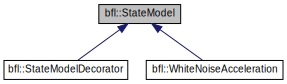
\includegraphics[width=350pt]{classbfl_1_1StateModel__inherit__graph}
\end{center}
\end{figure}
\subsection*{Public Member Functions}
\begin{DoxyCompactItemize}
\item 
virtual \mbox{\hyperlink{classbfl_1_1StateModel_ae07722f42306f297da2e55ce8cb0214a}{$\sim$\+State\+Model}} () noexcept
\item 
virtual void \mbox{\hyperlink{classbfl_1_1StateModel_a47a625abb7df9b7afa689ccb9aa11aee}{propagate}} (const Eigen\+::\+Ref$<$ const Eigen\+::\+Matrix\+Xf $>$ \&cur\+\_\+states, Eigen\+::\+Ref$<$ Eigen\+::\+Matrix\+Xf $>$ prop\+\_\+states)=0
\item 
virtual void \mbox{\hyperlink{classbfl_1_1StateModel_a3601485697ae3445ec7ca753dbeb035c}{motion}} (const Eigen\+::\+Ref$<$ const Eigen\+::\+Matrix\+Xf $>$ \&cur\+\_\+states, Eigen\+::\+Ref$<$ Eigen\+::\+Matrix\+Xf $>$ mot\+\_\+states)=0
\item 
virtual Eigen\+::\+Matrix\+Xf \mbox{\hyperlink{classbfl_1_1StateModel_ab1f0aa4c804b7de86c68294de3df76ee}{get\+Noise\+Sample}} (const int num)=0
\item 
virtual Eigen\+::\+Matrix\+Xf \mbox{\hyperlink{classbfl_1_1StateModel_a606efee8bf37606833c1ac75f2fbb357}{get\+Noise\+Covariance\+Matrix}} ()=0
\item 
virtual bool \mbox{\hyperlink{classbfl_1_1StateModel_ac86dcdad8f0bbfab39a23e592779feaa}{set\+Property}} (const std\+::string \&property)=0
\end{DoxyCompactItemize}


\subsection{Detailed Description}


Definition at line 11 of file State\+Model.\+h.



\subsection{Constructor \& Destructor Documentation}
\mbox{\Hypertarget{classbfl_1_1StateModel_ae07722f42306f297da2e55ce8cb0214a}\label{classbfl_1_1StateModel_ae07722f42306f297da2e55ce8cb0214a}} 
\index{bfl\+::\+State\+Model@{bfl\+::\+State\+Model}!````~State\+Model@{$\sim$\+State\+Model}}
\index{````~State\+Model@{$\sim$\+State\+Model}!bfl\+::\+State\+Model@{bfl\+::\+State\+Model}}
\subsubsection{\texorpdfstring{$\sim$\+State\+Model()}{~StateModel()}}
{\footnotesize\ttfamily virtual bfl\+::\+State\+Model\+::$\sim$\+State\+Model (\begin{DoxyParamCaption}{ }\end{DoxyParamCaption})\hspace{0.3cm}{\ttfamily [inline]}, {\ttfamily [virtual]}, {\ttfamily [noexcept]}}



Definition at line 14 of file State\+Model.\+h.



\subsection{Member Function Documentation}
\mbox{\Hypertarget{classbfl_1_1StateModel_a606efee8bf37606833c1ac75f2fbb357}\label{classbfl_1_1StateModel_a606efee8bf37606833c1ac75f2fbb357}} 
\index{bfl\+::\+State\+Model@{bfl\+::\+State\+Model}!get\+Noise\+Covariance\+Matrix@{get\+Noise\+Covariance\+Matrix}}
\index{get\+Noise\+Covariance\+Matrix@{get\+Noise\+Covariance\+Matrix}!bfl\+::\+State\+Model@{bfl\+::\+State\+Model}}
\subsubsection{\texorpdfstring{get\+Noise\+Covariance\+Matrix()}{getNoiseCovarianceMatrix()}}
{\footnotesize\ttfamily virtual Eigen\+::\+Matrix\+Xf bfl\+::\+State\+Model\+::get\+Noise\+Covariance\+Matrix (\begin{DoxyParamCaption}{ }\end{DoxyParamCaption})\hspace{0.3cm}{\ttfamily [pure virtual]}}



Implemented in \mbox{\hyperlink{classbfl_1_1WhiteNoiseAcceleration_a09c79104b153e6fb610bb2f1c6405636}{bfl\+::\+White\+Noise\+Acceleration}}, and \mbox{\hyperlink{classbfl_1_1StateModelDecorator_a1c64652f48c9463a2fa9b9e85d5ef0cf}{bfl\+::\+State\+Model\+Decorator}}.

\mbox{\Hypertarget{classbfl_1_1StateModel_ab1f0aa4c804b7de86c68294de3df76ee}\label{classbfl_1_1StateModel_ab1f0aa4c804b7de86c68294de3df76ee}} 
\index{bfl\+::\+State\+Model@{bfl\+::\+State\+Model}!get\+Noise\+Sample@{get\+Noise\+Sample}}
\index{get\+Noise\+Sample@{get\+Noise\+Sample}!bfl\+::\+State\+Model@{bfl\+::\+State\+Model}}
\subsubsection{\texorpdfstring{get\+Noise\+Sample()}{getNoiseSample()}}
{\footnotesize\ttfamily virtual Eigen\+::\+Matrix\+Xf bfl\+::\+State\+Model\+::get\+Noise\+Sample (\begin{DoxyParamCaption}\item[{const int}]{num }\end{DoxyParamCaption})\hspace{0.3cm}{\ttfamily [pure virtual]}}



Implemented in \mbox{\hyperlink{classbfl_1_1WhiteNoiseAcceleration_ac4bf4116d3a88435b9d070cbc8736656}{bfl\+::\+White\+Noise\+Acceleration}}, and \mbox{\hyperlink{classbfl_1_1StateModelDecorator_a3e29bad844203ffc3fe0c2bc445377e5}{bfl\+::\+State\+Model\+Decorator}}.

\mbox{\Hypertarget{classbfl_1_1StateModel_a3601485697ae3445ec7ca753dbeb035c}\label{classbfl_1_1StateModel_a3601485697ae3445ec7ca753dbeb035c}} 
\index{bfl\+::\+State\+Model@{bfl\+::\+State\+Model}!motion@{motion}}
\index{motion@{motion}!bfl\+::\+State\+Model@{bfl\+::\+State\+Model}}
\subsubsection{\texorpdfstring{motion()}{motion()}}
{\footnotesize\ttfamily virtual void bfl\+::\+State\+Model\+::motion (\begin{DoxyParamCaption}\item[{const Eigen\+::\+Ref$<$ const Eigen\+::\+Matrix\+Xf $>$ \&}]{cur\+\_\+states,  }\item[{Eigen\+::\+Ref$<$ Eigen\+::\+Matrix\+Xf $>$}]{mot\+\_\+states }\end{DoxyParamCaption})\hspace{0.3cm}{\ttfamily [pure virtual]}}



Implemented in \mbox{\hyperlink{classbfl_1_1WhiteNoiseAcceleration_addb79c08bdf08b89629bdcd24e46d1b8}{bfl\+::\+White\+Noise\+Acceleration}}, and \mbox{\hyperlink{classbfl_1_1StateModelDecorator_a0a645d8be4085ec13d9715a41c84a9b3}{bfl\+::\+State\+Model\+Decorator}}.

\mbox{\Hypertarget{classbfl_1_1StateModel_a47a625abb7df9b7afa689ccb9aa11aee}\label{classbfl_1_1StateModel_a47a625abb7df9b7afa689ccb9aa11aee}} 
\index{bfl\+::\+State\+Model@{bfl\+::\+State\+Model}!propagate@{propagate}}
\index{propagate@{propagate}!bfl\+::\+State\+Model@{bfl\+::\+State\+Model}}
\subsubsection{\texorpdfstring{propagate()}{propagate()}}
{\footnotesize\ttfamily virtual void bfl\+::\+State\+Model\+::propagate (\begin{DoxyParamCaption}\item[{const Eigen\+::\+Ref$<$ const Eigen\+::\+Matrix\+Xf $>$ \&}]{cur\+\_\+states,  }\item[{Eigen\+::\+Ref$<$ Eigen\+::\+Matrix\+Xf $>$}]{prop\+\_\+states }\end{DoxyParamCaption})\hspace{0.3cm}{\ttfamily [pure virtual]}}



Implemented in \mbox{\hyperlink{classbfl_1_1WhiteNoiseAcceleration_a1c2f938f535c20c78447a69c76c6896b}{bfl\+::\+White\+Noise\+Acceleration}}, and \mbox{\hyperlink{classbfl_1_1StateModelDecorator_a3780afac5fc0e542cf4517c2057f9957}{bfl\+::\+State\+Model\+Decorator}}.

\mbox{\Hypertarget{classbfl_1_1StateModel_ac86dcdad8f0bbfab39a23e592779feaa}\label{classbfl_1_1StateModel_ac86dcdad8f0bbfab39a23e592779feaa}} 
\index{bfl\+::\+State\+Model@{bfl\+::\+State\+Model}!set\+Property@{set\+Property}}
\index{set\+Property@{set\+Property}!bfl\+::\+State\+Model@{bfl\+::\+State\+Model}}
\subsubsection{\texorpdfstring{set\+Property()}{setProperty()}}
{\footnotesize\ttfamily virtual bool bfl\+::\+State\+Model\+::set\+Property (\begin{DoxyParamCaption}\item[{const std\+::string \&}]{property }\end{DoxyParamCaption})\hspace{0.3cm}{\ttfamily [pure virtual]}}



Implemented in \mbox{\hyperlink{classbfl_1_1WhiteNoiseAcceleration_a0203b47074e0680852f53dcba8a7a627}{bfl\+::\+White\+Noise\+Acceleration}}, and \mbox{\hyperlink{classbfl_1_1StateModelDecorator_ad292f3b665c1adf20a1f32dc8a065fec}{bfl\+::\+State\+Model\+Decorator}}.



The documentation for this class was generated from the following file\+:\begin{DoxyCompactItemize}
\item 
C\+:/\+Users/cfantacci/\+Git\+Hub/bayes-\/filters-\/lib/src/\+Bayes\+Filters/include/\+Bayes\+Filters/\mbox{\hyperlink{StateModel_8h}{State\+Model.\+h}}\end{DoxyCompactItemize}

\hypertarget{classbfl_1_1StateModelDecorator}{}\section{bfl\+:\+:State\+Model\+Decorator Class Reference}
\label{classbfl_1_1StateModelDecorator}\index{bfl\+::\+State\+Model\+Decorator@{bfl\+::\+State\+Model\+Decorator}}


{\ttfamily \#include $<$State\+Model\+Decorator.\+h$>$}



Inheritance diagram for bfl\+:\+:State\+Model\+Decorator\+:
\nopagebreak
\begin{figure}[H]
\begin{center}
\leavevmode
\includegraphics[width=204pt]{classbfl_1_1StateModelDecorator__inherit__graph}
\end{center}
\end{figure}
\subsection*{Public Member Functions}
\begin{DoxyCompactItemize}
\item 
void \mbox{\hyperlink{classbfl_1_1StateModelDecorator_a3780afac5fc0e542cf4517c2057f9957}{propagate}} (const Eigen\+::\+Ref$<$ const Eigen\+::\+Matrix\+Xf $>$ \&cur\+\_\+states, Eigen\+::\+Ref$<$ Eigen\+::\+Matrix\+Xf $>$ prop\+\_\+states) override
\item 
void \mbox{\hyperlink{classbfl_1_1StateModelDecorator_a0a645d8be4085ec13d9715a41c84a9b3}{motion}} (const Eigen\+::\+Ref$<$ const Eigen\+::\+Matrix\+Xf $>$ \&cur\+\_\+states, Eigen\+::\+Ref$<$ Eigen\+::\+Matrix\+Xf $>$ mot\+\_\+states) override
\item 
Eigen\+::\+Matrix\+Xf \mbox{\hyperlink{classbfl_1_1StateModelDecorator_a3e29bad844203ffc3fe0c2bc445377e5}{get\+Noise\+Sample}} (const int num) override
\item 
Eigen\+::\+Matrix\+Xf \mbox{\hyperlink{classbfl_1_1StateModelDecorator_a1c64652f48c9463a2fa9b9e85d5ef0cf}{get\+Noise\+Covariance\+Matrix}} () override
\item 
bool \mbox{\hyperlink{classbfl_1_1StateModelDecorator_ad292f3b665c1adf20a1f32dc8a065fec}{set\+Property}} (const std\+::string \&property) override
\end{DoxyCompactItemize}
\subsection*{Protected Member Functions}
\begin{DoxyCompactItemize}
\item 
\mbox{\hyperlink{classbfl_1_1StateModelDecorator_aeb562beb07afb133ca101245f7f16af8}{State\+Model\+Decorator}} (std\+::unique\+\_\+ptr$<$ \mbox{\hyperlink{classbfl_1_1StateModel}{State\+Model}} $>$ state\+\_\+model) noexcept
\item 
\mbox{\hyperlink{classbfl_1_1StateModelDecorator_a29a4fd2af9aa020b85cc73b672c87bfd}{State\+Model\+Decorator}} (\mbox{\hyperlink{classbfl_1_1StateModelDecorator}{State\+Model\+Decorator}} \&\&state\+\_\+model) noexcept
\item 
virtual \mbox{\hyperlink{classbfl_1_1StateModelDecorator_a5bcacbbecd5354161dee32eaaec8bfae}{$\sim$\+State\+Model\+Decorator}} () noexcept
\item 
\mbox{\hyperlink{classbfl_1_1StateModelDecorator}{State\+Model\+Decorator}} \& \mbox{\hyperlink{classbfl_1_1StateModelDecorator_a5f7ab9c56ebbf7f653014933d688339b}{operator=}} (\mbox{\hyperlink{classbfl_1_1StateModelDecorator}{State\+Model\+Decorator}} \&\&state\+\_\+model) noexcept
\end{DoxyCompactItemize}
\subsection*{Private Attributes}
\begin{DoxyCompactItemize}
\item 
std\+::unique\+\_\+ptr$<$ \mbox{\hyperlink{classbfl_1_1StateModel}{State\+Model}} $>$ \mbox{\hyperlink{classbfl_1_1StateModelDecorator_acd7df6c203047dfa16ef78dd34c1b769}{state\+\_\+model\+\_\+}}
\end{DoxyCompactItemize}


\subsection{Detailed Description}


Definition at line 13 of file State\+Model\+Decorator.\+h.



\subsection{Constructor \& Destructor Documentation}
\mbox{\Hypertarget{classbfl_1_1StateModelDecorator_aeb562beb07afb133ca101245f7f16af8}\label{classbfl_1_1StateModelDecorator_aeb562beb07afb133ca101245f7f16af8}} 
\index{bfl\+::\+State\+Model\+Decorator@{bfl\+::\+State\+Model\+Decorator}!State\+Model\+Decorator@{State\+Model\+Decorator}}
\index{State\+Model\+Decorator@{State\+Model\+Decorator}!bfl\+::\+State\+Model\+Decorator@{bfl\+::\+State\+Model\+Decorator}}
\subsubsection{\texorpdfstring{State\+Model\+Decorator()}{StateModelDecorator()}\hspace{0.1cm}{\footnotesize\ttfamily [1/2]}}
{\footnotesize\ttfamily State\+Model\+Decorator\+::\+State\+Model\+Decorator (\begin{DoxyParamCaption}\item[{std\+::unique\+\_\+ptr$<$ \mbox{\hyperlink{classbfl_1_1StateModel}{State\+Model}} $>$}]{state\+\_\+model }\end{DoxyParamCaption})\hspace{0.3cm}{\ttfamily [protected]}, {\ttfamily [noexcept]}}



Definition at line 7 of file State\+Model\+Decorator.\+cpp.

\mbox{\Hypertarget{classbfl_1_1StateModelDecorator_a29a4fd2af9aa020b85cc73b672c87bfd}\label{classbfl_1_1StateModelDecorator_a29a4fd2af9aa020b85cc73b672c87bfd}} 
\index{bfl\+::\+State\+Model\+Decorator@{bfl\+::\+State\+Model\+Decorator}!State\+Model\+Decorator@{State\+Model\+Decorator}}
\index{State\+Model\+Decorator@{State\+Model\+Decorator}!bfl\+::\+State\+Model\+Decorator@{bfl\+::\+State\+Model\+Decorator}}
\subsubsection{\texorpdfstring{State\+Model\+Decorator()}{StateModelDecorator()}\hspace{0.1cm}{\footnotesize\ttfamily [2/2]}}
{\footnotesize\ttfamily State\+Model\+Decorator\+::\+State\+Model\+Decorator (\begin{DoxyParamCaption}\item[{\mbox{\hyperlink{classbfl_1_1StateModelDecorator}{State\+Model\+Decorator}} \&\&}]{state\+\_\+model }\end{DoxyParamCaption})\hspace{0.3cm}{\ttfamily [protected]}, {\ttfamily [noexcept]}}



Definition at line 11 of file State\+Model\+Decorator.\+cpp.

\mbox{\Hypertarget{classbfl_1_1StateModelDecorator_a5bcacbbecd5354161dee32eaaec8bfae}\label{classbfl_1_1StateModelDecorator_a5bcacbbecd5354161dee32eaaec8bfae}} 
\index{bfl\+::\+State\+Model\+Decorator@{bfl\+::\+State\+Model\+Decorator}!````~State\+Model\+Decorator@{$\sim$\+State\+Model\+Decorator}}
\index{````~State\+Model\+Decorator@{$\sim$\+State\+Model\+Decorator}!bfl\+::\+State\+Model\+Decorator@{bfl\+::\+State\+Model\+Decorator}}
\subsubsection{\texorpdfstring{$\sim$\+State\+Model\+Decorator()}{~StateModelDecorator()}}
{\footnotesize\ttfamily State\+Model\+Decorator\+::$\sim$\+State\+Model\+Decorator (\begin{DoxyParamCaption}{ }\end{DoxyParamCaption})\hspace{0.3cm}{\ttfamily [protected]}, {\ttfamily [virtual]}, {\ttfamily [noexcept]}}



Definition at line 15 of file State\+Model\+Decorator.\+cpp.



\subsection{Member Function Documentation}
\mbox{\Hypertarget{classbfl_1_1StateModelDecorator_a1c64652f48c9463a2fa9b9e85d5ef0cf}\label{classbfl_1_1StateModelDecorator_a1c64652f48c9463a2fa9b9e85d5ef0cf}} 
\index{bfl\+::\+State\+Model\+Decorator@{bfl\+::\+State\+Model\+Decorator}!get\+Noise\+Covariance\+Matrix@{get\+Noise\+Covariance\+Matrix}}
\index{get\+Noise\+Covariance\+Matrix@{get\+Noise\+Covariance\+Matrix}!bfl\+::\+State\+Model\+Decorator@{bfl\+::\+State\+Model\+Decorator}}
\subsubsection{\texorpdfstring{get\+Noise\+Covariance\+Matrix()}{getNoiseCovarianceMatrix()}}
{\footnotesize\ttfamily Matrix\+Xf State\+Model\+Decorator\+::get\+Noise\+Covariance\+Matrix (\begin{DoxyParamCaption}{ }\end{DoxyParamCaption})\hspace{0.3cm}{\ttfamily [override]}, {\ttfamily [virtual]}}



Implements \mbox{\hyperlink{classbfl_1_1StateModel_a606efee8bf37606833c1ac75f2fbb357}{bfl\+::\+State\+Model}}.



Definition at line 44 of file State\+Model\+Decorator.\+cpp.

\mbox{\Hypertarget{classbfl_1_1StateModelDecorator_a3e29bad844203ffc3fe0c2bc445377e5}\label{classbfl_1_1StateModelDecorator_a3e29bad844203ffc3fe0c2bc445377e5}} 
\index{bfl\+::\+State\+Model\+Decorator@{bfl\+::\+State\+Model\+Decorator}!get\+Noise\+Sample@{get\+Noise\+Sample}}
\index{get\+Noise\+Sample@{get\+Noise\+Sample}!bfl\+::\+State\+Model\+Decorator@{bfl\+::\+State\+Model\+Decorator}}
\subsubsection{\texorpdfstring{get\+Noise\+Sample()}{getNoiseSample()}}
{\footnotesize\ttfamily Matrix\+Xf State\+Model\+Decorator\+::get\+Noise\+Sample (\begin{DoxyParamCaption}\item[{const int}]{num }\end{DoxyParamCaption})\hspace{0.3cm}{\ttfamily [override]}, {\ttfamily [virtual]}}



Implements \mbox{\hyperlink{classbfl_1_1StateModel_ab1f0aa4c804b7de86c68294de3df76ee}{bfl\+::\+State\+Model}}.



Definition at line 38 of file State\+Model\+Decorator.\+cpp.

\mbox{\Hypertarget{classbfl_1_1StateModelDecorator_a0a645d8be4085ec13d9715a41c84a9b3}\label{classbfl_1_1StateModelDecorator_a0a645d8be4085ec13d9715a41c84a9b3}} 
\index{bfl\+::\+State\+Model\+Decorator@{bfl\+::\+State\+Model\+Decorator}!motion@{motion}}
\index{motion@{motion}!bfl\+::\+State\+Model\+Decorator@{bfl\+::\+State\+Model\+Decorator}}
\subsubsection{\texorpdfstring{motion()}{motion()}}
{\footnotesize\ttfamily void State\+Model\+Decorator\+::motion (\begin{DoxyParamCaption}\item[{const Eigen\+::\+Ref$<$ const Eigen\+::\+Matrix\+Xf $>$ \&}]{cur\+\_\+states,  }\item[{Eigen\+::\+Ref$<$ Eigen\+::\+Matrix\+Xf $>$}]{mot\+\_\+states }\end{DoxyParamCaption})\hspace{0.3cm}{\ttfamily [override]}, {\ttfamily [virtual]}}



Implements \mbox{\hyperlink{classbfl_1_1StateModel_a3601485697ae3445ec7ca753dbeb035c}{bfl\+::\+State\+Model}}.



Definition at line 32 of file State\+Model\+Decorator.\+cpp.

\mbox{\Hypertarget{classbfl_1_1StateModelDecorator_a5f7ab9c56ebbf7f653014933d688339b}\label{classbfl_1_1StateModelDecorator_a5f7ab9c56ebbf7f653014933d688339b}} 
\index{bfl\+::\+State\+Model\+Decorator@{bfl\+::\+State\+Model\+Decorator}!operator=@{operator=}}
\index{operator=@{operator=}!bfl\+::\+State\+Model\+Decorator@{bfl\+::\+State\+Model\+Decorator}}
\subsubsection{\texorpdfstring{operator=()}{operator=()}}
{\footnotesize\ttfamily \mbox{\hyperlink{classbfl_1_1StateModelDecorator}{State\+Model\+Decorator}} \& State\+Model\+Decorator\+::operator= (\begin{DoxyParamCaption}\item[{\mbox{\hyperlink{classbfl_1_1StateModelDecorator}{State\+Model\+Decorator}} \&\&}]{state\+\_\+model }\end{DoxyParamCaption})\hspace{0.3cm}{\ttfamily [protected]}, {\ttfamily [noexcept]}}



Definition at line 18 of file State\+Model\+Decorator.\+cpp.

\mbox{\Hypertarget{classbfl_1_1StateModelDecorator_a3780afac5fc0e542cf4517c2057f9957}\label{classbfl_1_1StateModelDecorator_a3780afac5fc0e542cf4517c2057f9957}} 
\index{bfl\+::\+State\+Model\+Decorator@{bfl\+::\+State\+Model\+Decorator}!propagate@{propagate}}
\index{propagate@{propagate}!bfl\+::\+State\+Model\+Decorator@{bfl\+::\+State\+Model\+Decorator}}
\subsubsection{\texorpdfstring{propagate()}{propagate()}}
{\footnotesize\ttfamily void State\+Model\+Decorator\+::propagate (\begin{DoxyParamCaption}\item[{const Eigen\+::\+Ref$<$ const Eigen\+::\+Matrix\+Xf $>$ \&}]{cur\+\_\+states,  }\item[{Eigen\+::\+Ref$<$ Eigen\+::\+Matrix\+Xf $>$}]{prop\+\_\+states }\end{DoxyParamCaption})\hspace{0.3cm}{\ttfamily [override]}, {\ttfamily [virtual]}}



Implements \mbox{\hyperlink{classbfl_1_1StateModel_a47a625abb7df9b7afa689ccb9aa11aee}{bfl\+::\+State\+Model}}.



Definition at line 26 of file State\+Model\+Decorator.\+cpp.

\mbox{\Hypertarget{classbfl_1_1StateModelDecorator_ad292f3b665c1adf20a1f32dc8a065fec}\label{classbfl_1_1StateModelDecorator_ad292f3b665c1adf20a1f32dc8a065fec}} 
\index{bfl\+::\+State\+Model\+Decorator@{bfl\+::\+State\+Model\+Decorator}!set\+Property@{set\+Property}}
\index{set\+Property@{set\+Property}!bfl\+::\+State\+Model\+Decorator@{bfl\+::\+State\+Model\+Decorator}}
\subsubsection{\texorpdfstring{set\+Property()}{setProperty()}}
{\footnotesize\ttfamily bool State\+Model\+Decorator\+::set\+Property (\begin{DoxyParamCaption}\item[{const std\+::string \&}]{property }\end{DoxyParamCaption})\hspace{0.3cm}{\ttfamily [override]}, {\ttfamily [virtual]}}



Implements \mbox{\hyperlink{classbfl_1_1StateModel_ac86dcdad8f0bbfab39a23e592779feaa}{bfl\+::\+State\+Model}}.



Definition at line 50 of file State\+Model\+Decorator.\+cpp.



\subsection{Member Data Documentation}
\mbox{\Hypertarget{classbfl_1_1StateModelDecorator_acd7df6c203047dfa16ef78dd34c1b769}\label{classbfl_1_1StateModelDecorator_acd7df6c203047dfa16ef78dd34c1b769}} 
\index{bfl\+::\+State\+Model\+Decorator@{bfl\+::\+State\+Model\+Decorator}!state\+\_\+model\+\_\+@{state\+\_\+model\+\_\+}}
\index{state\+\_\+model\+\_\+@{state\+\_\+model\+\_\+}!bfl\+::\+State\+Model\+Decorator@{bfl\+::\+State\+Model\+Decorator}}
\subsubsection{\texorpdfstring{state\+\_\+model\+\_\+}{state\_model\_}}
{\footnotesize\ttfamily std\+::unique\+\_\+ptr$<$\mbox{\hyperlink{classbfl_1_1StateModel}{State\+Model}}$>$ bfl\+::\+State\+Model\+Decorator\+::state\+\_\+model\+\_\+\hspace{0.3cm}{\ttfamily [private]}}



Definition at line 36 of file State\+Model\+Decorator.\+h.



The documentation for this class was generated from the following files\+:\begin{DoxyCompactItemize}
\item 
C\+:/\+Users/cfantacci/\+Git\+Hub/bayes-\/filters-\/lib/src/\+Bayes\+Filters/include/\+Bayes\+Filters/\mbox{\hyperlink{StateModelDecorator_8h}{State\+Model\+Decorator.\+h}}\item 
C\+:/\+Users/cfantacci/\+Git\+Hub/bayes-\/filters-\/lib/src/\+Bayes\+Filters/src/\mbox{\hyperlink{StateModelDecorator_8cpp}{State\+Model\+Decorator.\+cpp}}\end{DoxyCompactItemize}

\hypertarget{classbfl_1_1UnscentedKalmanFilter}{}\section{bfl\+:\+:Unscented\+Kalman\+Filter Class Reference}
\label{classbfl_1_1UnscentedKalmanFilter}\index{bfl\+::\+Unscented\+Kalman\+Filter@{bfl\+::\+Unscented\+Kalman\+Filter}}


{\ttfamily \#include $<$Unscented\+Kalman\+Filter.\+h$>$}



Inheritance diagram for bfl\+:\+:Unscented\+Kalman\+Filter\+:
\nopagebreak
\begin{figure}[H]
\begin{center}
\leavevmode
\includegraphics[width=214pt]{classbfl_1_1UnscentedKalmanFilter__inherit__graph}
\end{center}
\end{figure}
\subsection*{Public Member Functions}
\begin{DoxyCompactItemize}
\item 
\mbox{\hyperlink{classbfl_1_1UnscentedKalmanFilter_a18a80ca47ed5440b116e1abd8be406b6}{Unscented\+Kalman\+Filter}} ()
\item 
virtual \mbox{\hyperlink{classbfl_1_1UnscentedKalmanFilter_ac3b1c8406622c7295da808fe95e4c170}{$\sim$\+Unscented\+Kalman\+Filter}} () noexcept
\item 
void \mbox{\hyperlink{classbfl_1_1UnscentedKalmanFilter_acd5cfc6344d9ce24fb980aa22ecf4895}{initialization}} () override
\item 
void \mbox{\hyperlink{classbfl_1_1UnscentedKalmanFilter_a169451bb711a03ad2dc28a40e3ad867f}{filtering\+Step}} () override
\item 
void \mbox{\hyperlink{classbfl_1_1UnscentedKalmanFilter_ad25c4f9143bbe834b3adfc81c78b6743}{get\+Result}} () override
\item 
bool \mbox{\hyperlink{classbfl_1_1FilteringAlgorithm_a96651f8464190c0a56d79219a1017147}{boot}} ()
\item 
void \mbox{\hyperlink{classbfl_1_1FilteringAlgorithm_a009cbe5f4bbb16967f6c6ddcaed8fbb1}{run}} ()
\item 
bool \mbox{\hyperlink{classbfl_1_1FilteringAlgorithm_a40372c24fa050eb0274371172df0a244}{wait}} ()
\item 
void \mbox{\hyperlink{classbfl_1_1FilteringAlgorithm_a2403c62fbd7bd7f5cda56a84f5f30331}{reset}} ()
\item 
void \mbox{\hyperlink{classbfl_1_1FilteringAlgorithm_a6022859aa985474fb997343cc935b11e}{reboot}} ()
\item 
bool \mbox{\hyperlink{classbfl_1_1FilteringAlgorithm_a1dc912d89ee8f96d4f3e8209865c5308}{teardown}} ()
\item 
unsigned int \mbox{\hyperlink{classbfl_1_1FilteringAlgorithm_a8c43b1f3dac30934c0a03de348d4a29d}{get\+Filtering\+Step}} ()
\item 
bool \mbox{\hyperlink{classbfl_1_1FilteringAlgorithm_a5cfecab2c778620e2557237472bb1721}{is\+Running}} ()
\item 
virtual bool \mbox{\hyperlink{classbfl_1_1FilteringAlgorithm_ac8a718a614905d89d6a43bbbc70d68b2}{skip}} (const std\+::string \&what\+\_\+step, const bool status)=0
\end{DoxyCompactItemize}
\subsection*{Protected Member Functions}
\begin{DoxyCompactItemize}
\item 
virtual bool \mbox{\hyperlink{classbfl_1_1FilteringAlgorithm_a5fc12882356f6906b102fbfff2bc4b7c}{run\+Condition}} ()=0
\end{DoxyCompactItemize}


\subsection{Detailed Description}


Definition at line 11 of file Unscented\+Kalman\+Filter.\+h.



\subsection{Constructor \& Destructor Documentation}
\mbox{\Hypertarget{classbfl_1_1UnscentedKalmanFilter_a18a80ca47ed5440b116e1abd8be406b6}\label{classbfl_1_1UnscentedKalmanFilter_a18a80ca47ed5440b116e1abd8be406b6}} 
\index{bfl\+::\+Unscented\+Kalman\+Filter@{bfl\+::\+Unscented\+Kalman\+Filter}!Unscented\+Kalman\+Filter@{Unscented\+Kalman\+Filter}}
\index{Unscented\+Kalman\+Filter@{Unscented\+Kalman\+Filter}!bfl\+::\+Unscented\+Kalman\+Filter@{bfl\+::\+Unscented\+Kalman\+Filter}}
\subsubsection{\texorpdfstring{Unscented\+Kalman\+Filter()}{UnscentedKalmanFilter()}}
{\footnotesize\ttfamily Unscented\+Kalman\+Filter\+::\+Unscented\+Kalman\+Filter (\begin{DoxyParamCaption}{ }\end{DoxyParamCaption})}



Definition at line 6 of file Unscented\+Kalman\+Filter.\+cpp.

\mbox{\Hypertarget{classbfl_1_1UnscentedKalmanFilter_ac3b1c8406622c7295da808fe95e4c170}\label{classbfl_1_1UnscentedKalmanFilter_ac3b1c8406622c7295da808fe95e4c170}} 
\index{bfl\+::\+Unscented\+Kalman\+Filter@{bfl\+::\+Unscented\+Kalman\+Filter}!````~Unscented\+Kalman\+Filter@{$\sim$\+Unscented\+Kalman\+Filter}}
\index{````~Unscented\+Kalman\+Filter@{$\sim$\+Unscented\+Kalman\+Filter}!bfl\+::\+Unscented\+Kalman\+Filter@{bfl\+::\+Unscented\+Kalman\+Filter}}
\subsubsection{\texorpdfstring{$\sim$\+Unscented\+Kalman\+Filter()}{~UnscentedKalmanFilter()}}
{\footnotesize\ttfamily Unscented\+Kalman\+Filter\+::$\sim$\+Unscented\+Kalman\+Filter (\begin{DoxyParamCaption}{ }\end{DoxyParamCaption})\hspace{0.3cm}{\ttfamily [virtual]}, {\ttfamily [noexcept]}}



Definition at line 9 of file Unscented\+Kalman\+Filter.\+cpp.



\subsection{Member Function Documentation}
\mbox{\Hypertarget{classbfl_1_1FilteringAlgorithm_a96651f8464190c0a56d79219a1017147}\label{classbfl_1_1FilteringAlgorithm_a96651f8464190c0a56d79219a1017147}} 
\index{bfl\+::\+Unscented\+Kalman\+Filter@{bfl\+::\+Unscented\+Kalman\+Filter}!boot@{boot}}
\index{boot@{boot}!bfl\+::\+Unscented\+Kalman\+Filter@{bfl\+::\+Unscented\+Kalman\+Filter}}
\subsubsection{\texorpdfstring{boot()}{boot()}}
{\footnotesize\ttfamily bool Filtering\+Algorithm\+::boot (\begin{DoxyParamCaption}{ }\end{DoxyParamCaption})\hspace{0.3cm}{\ttfamily [inherited]}}



Definition at line 8 of file Filtering\+Algorithm.\+cpp.



References bfl\+::\+Filtering\+Algorithm\+::filtering\+\_\+thread\+\_\+, and bfl\+::\+Filtering\+Algorithm\+::filtering\+Recursion().

Here is the call graph for this function\+:
\nopagebreak
\begin{figure}[H]
\begin{center}
\leavevmode
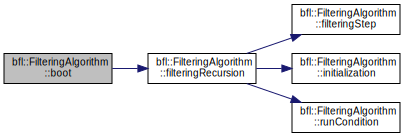
\includegraphics[width=350pt]{classbfl_1_1FilteringAlgorithm_a96651f8464190c0a56d79219a1017147_cgraph}
\end{center}
\end{figure}
\mbox{\Hypertarget{classbfl_1_1UnscentedKalmanFilter_a169451bb711a03ad2dc28a40e3ad867f}\label{classbfl_1_1UnscentedKalmanFilter_a169451bb711a03ad2dc28a40e3ad867f}} 
\index{bfl\+::\+Unscented\+Kalman\+Filter@{bfl\+::\+Unscented\+Kalman\+Filter}!filtering\+Step@{filtering\+Step}}
\index{filtering\+Step@{filtering\+Step}!bfl\+::\+Unscented\+Kalman\+Filter@{bfl\+::\+Unscented\+Kalman\+Filter}}
\subsubsection{\texorpdfstring{filtering\+Step()}{filteringStep()}}
{\footnotesize\ttfamily void Unscented\+Kalman\+Filter\+::filtering\+Step (\begin{DoxyParamCaption}{ }\end{DoxyParamCaption})\hspace{0.3cm}{\ttfamily [override]}, {\ttfamily [virtual]}}



Implements \mbox{\hyperlink{classbfl_1_1FilteringAlgorithm_ab3bceb43b5810a4bf1da884b8a0b145a}{bfl\+::\+Filtering\+Algorithm}}.



Definition at line 15 of file Unscented\+Kalman\+Filter.\+cpp.

\mbox{\Hypertarget{classbfl_1_1FilteringAlgorithm_a8c43b1f3dac30934c0a03de348d4a29d}\label{classbfl_1_1FilteringAlgorithm_a8c43b1f3dac30934c0a03de348d4a29d}} 
\index{bfl\+::\+Unscented\+Kalman\+Filter@{bfl\+::\+Unscented\+Kalman\+Filter}!get\+Filtering\+Step@{get\+Filtering\+Step}}
\index{get\+Filtering\+Step@{get\+Filtering\+Step}!bfl\+::\+Unscented\+Kalman\+Filter@{bfl\+::\+Unscented\+Kalman\+Filter}}
\subsubsection{\texorpdfstring{get\+Filtering\+Step()}{getFilteringStep()}}
{\footnotesize\ttfamily unsigned int Filtering\+Algorithm\+::get\+Filtering\+Step (\begin{DoxyParamCaption}{ }\end{DoxyParamCaption})\hspace{0.3cm}{\ttfamily [inherited]}}



Definition at line 86 of file Filtering\+Algorithm.\+cpp.



References bfl\+::\+Filtering\+Algorithm\+::filtering\+\_\+step\+\_\+.

\mbox{\Hypertarget{classbfl_1_1UnscentedKalmanFilter_ad25c4f9143bbe834b3adfc81c78b6743}\label{classbfl_1_1UnscentedKalmanFilter_ad25c4f9143bbe834b3adfc81c78b6743}} 
\index{bfl\+::\+Unscented\+Kalman\+Filter@{bfl\+::\+Unscented\+Kalman\+Filter}!get\+Result@{get\+Result}}
\index{get\+Result@{get\+Result}!bfl\+::\+Unscented\+Kalman\+Filter@{bfl\+::\+Unscented\+Kalman\+Filter}}
\subsubsection{\texorpdfstring{get\+Result()}{getResult()}}
{\footnotesize\ttfamily void Unscented\+Kalman\+Filter\+::get\+Result (\begin{DoxyParamCaption}{ }\end{DoxyParamCaption})\hspace{0.3cm}{\ttfamily [override]}, {\ttfamily [virtual]}}



Implements \mbox{\hyperlink{classbfl_1_1FilteringAlgorithm_acdfebf68405a427491e4dd9d020ae09b}{bfl\+::\+Filtering\+Algorithm}}.



Definition at line 18 of file Unscented\+Kalman\+Filter.\+cpp.

\mbox{\Hypertarget{classbfl_1_1UnscentedKalmanFilter_acd5cfc6344d9ce24fb980aa22ecf4895}\label{classbfl_1_1UnscentedKalmanFilter_acd5cfc6344d9ce24fb980aa22ecf4895}} 
\index{bfl\+::\+Unscented\+Kalman\+Filter@{bfl\+::\+Unscented\+Kalman\+Filter}!initialization@{initialization}}
\index{initialization@{initialization}!bfl\+::\+Unscented\+Kalman\+Filter@{bfl\+::\+Unscented\+Kalman\+Filter}}
\subsubsection{\texorpdfstring{initialization()}{initialization()}}
{\footnotesize\ttfamily void Unscented\+Kalman\+Filter\+::initialization (\begin{DoxyParamCaption}{ }\end{DoxyParamCaption})\hspace{0.3cm}{\ttfamily [override]}, {\ttfamily [virtual]}}



Implements \mbox{\hyperlink{classbfl_1_1FilteringAlgorithm_af2a072aa51407fe5544bdbb7ce466e2a}{bfl\+::\+Filtering\+Algorithm}}.



Definition at line 12 of file Unscented\+Kalman\+Filter.\+cpp.

\mbox{\Hypertarget{classbfl_1_1FilteringAlgorithm_a5cfecab2c778620e2557237472bb1721}\label{classbfl_1_1FilteringAlgorithm_a5cfecab2c778620e2557237472bb1721}} 
\index{bfl\+::\+Unscented\+Kalman\+Filter@{bfl\+::\+Unscented\+Kalman\+Filter}!is\+Running@{is\+Running}}
\index{is\+Running@{is\+Running}!bfl\+::\+Unscented\+Kalman\+Filter@{bfl\+::\+Unscented\+Kalman\+Filter}}
\subsubsection{\texorpdfstring{is\+Running()}{isRunning()}}
{\footnotesize\ttfamily bool Filtering\+Algorithm\+::is\+Running (\begin{DoxyParamCaption}{ }\end{DoxyParamCaption})\hspace{0.3cm}{\ttfamily [inherited]}}



Definition at line 92 of file Filtering\+Algorithm.\+cpp.



References bfl\+::\+Filtering\+Algorithm\+::run\+\_\+.

\mbox{\Hypertarget{classbfl_1_1FilteringAlgorithm_a6022859aa985474fb997343cc935b11e}\label{classbfl_1_1FilteringAlgorithm_a6022859aa985474fb997343cc935b11e}} 
\index{bfl\+::\+Unscented\+Kalman\+Filter@{bfl\+::\+Unscented\+Kalman\+Filter}!reboot@{reboot}}
\index{reboot@{reboot}!bfl\+::\+Unscented\+Kalman\+Filter@{bfl\+::\+Unscented\+Kalman\+Filter}}
\subsubsection{\texorpdfstring{reboot()}{reboot()}}
{\footnotesize\ttfamily void Filtering\+Algorithm\+::reboot (\begin{DoxyParamCaption}{ }\end{DoxyParamCaption})\hspace{0.3cm}{\ttfamily [inherited]}}



Definition at line 66 of file Filtering\+Algorithm.\+cpp.



References bfl\+::\+Filtering\+Algorithm\+::cv\+\_\+run\+\_\+, bfl\+::\+Filtering\+Algorithm\+::mtx\+\_\+run\+\_\+, bfl\+::\+Filtering\+Algorithm\+::reset\+\_\+, and bfl\+::\+Filtering\+Algorithm\+::run\+\_\+.

\mbox{\Hypertarget{classbfl_1_1FilteringAlgorithm_a2403c62fbd7bd7f5cda56a84f5f30331}\label{classbfl_1_1FilteringAlgorithm_a2403c62fbd7bd7f5cda56a84f5f30331}} 
\index{bfl\+::\+Unscented\+Kalman\+Filter@{bfl\+::\+Unscented\+Kalman\+Filter}!reset@{reset}}
\index{reset@{reset}!bfl\+::\+Unscented\+Kalman\+Filter@{bfl\+::\+Unscented\+Kalman\+Filter}}
\subsubsection{\texorpdfstring{reset()}{reset()}}
{\footnotesize\ttfamily void Filtering\+Algorithm\+::reset (\begin{DoxyParamCaption}{ }\end{DoxyParamCaption})\hspace{0.3cm}{\ttfamily [inherited]}}



Definition at line 60 of file Filtering\+Algorithm.\+cpp.



References bfl\+::\+Filtering\+Algorithm\+::reset\+\_\+.

\mbox{\Hypertarget{classbfl_1_1FilteringAlgorithm_a009cbe5f4bbb16967f6c6ddcaed8fbb1}\label{classbfl_1_1FilteringAlgorithm_a009cbe5f4bbb16967f6c6ddcaed8fbb1}} 
\index{bfl\+::\+Unscented\+Kalman\+Filter@{bfl\+::\+Unscented\+Kalman\+Filter}!run@{run}}
\index{run@{run}!bfl\+::\+Unscented\+Kalman\+Filter@{bfl\+::\+Unscented\+Kalman\+Filter}}
\subsubsection{\texorpdfstring{run()}{run()}}
{\footnotesize\ttfamily void Filtering\+Algorithm\+::run (\begin{DoxyParamCaption}{ }\end{DoxyParamCaption})\hspace{0.3cm}{\ttfamily [inherited]}}



Definition at line 26 of file Filtering\+Algorithm.\+cpp.



References bfl\+::\+Filtering\+Algorithm\+::cv\+\_\+run\+\_\+, bfl\+::\+Filtering\+Algorithm\+::mtx\+\_\+run\+\_\+, and bfl\+::\+Filtering\+Algorithm\+::run\+\_\+.

\mbox{\Hypertarget{classbfl_1_1FilteringAlgorithm_a5fc12882356f6906b102fbfff2bc4b7c}\label{classbfl_1_1FilteringAlgorithm_a5fc12882356f6906b102fbfff2bc4b7c}} 
\index{bfl\+::\+Unscented\+Kalman\+Filter@{bfl\+::\+Unscented\+Kalman\+Filter}!run\+Condition@{run\+Condition}}
\index{run\+Condition@{run\+Condition}!bfl\+::\+Unscented\+Kalman\+Filter@{bfl\+::\+Unscented\+Kalman\+Filter}}
\subsubsection{\texorpdfstring{run\+Condition()}{runCondition()}}
{\footnotesize\ttfamily virtual bool bfl\+::\+Filtering\+Algorithm\+::run\+Condition (\begin{DoxyParamCaption}{ }\end{DoxyParamCaption})\hspace{0.3cm}{\ttfamily [protected]}, {\ttfamily [pure virtual]}, {\ttfamily [inherited]}}



Implemented in \mbox{\hyperlink{classbfl_1_1SIS_afb7cff1f7dae80e0e4ca84c925ca3ac3}{bfl\+::\+S\+IS}}.



Referenced by bfl\+::\+Filtering\+Algorithm\+::filtering\+Recursion().

\mbox{\Hypertarget{classbfl_1_1FilteringAlgorithm_ac8a718a614905d89d6a43bbbc70d68b2}\label{classbfl_1_1FilteringAlgorithm_ac8a718a614905d89d6a43bbbc70d68b2}} 
\index{bfl\+::\+Unscented\+Kalman\+Filter@{bfl\+::\+Unscented\+Kalman\+Filter}!skip@{skip}}
\index{skip@{skip}!bfl\+::\+Unscented\+Kalman\+Filter@{bfl\+::\+Unscented\+Kalman\+Filter}}
\subsubsection{\texorpdfstring{skip()}{skip()}}
{\footnotesize\ttfamily virtual bool bfl\+::\+Filtering\+Algorithm\+::skip (\begin{DoxyParamCaption}\item[{const std\+::string \&}]{what\+\_\+step,  }\item[{const bool}]{status }\end{DoxyParamCaption})\hspace{0.3cm}{\ttfamily [pure virtual]}, {\ttfamily [inherited]}}



Implemented in \mbox{\hyperlink{classbfl_1_1ParticleFilter_a2d7a5e7aaad179037273d35be229056d}{bfl\+::\+Particle\+Filter}}, and \mbox{\hyperlink{classbfl_1_1VisualParticleFilter_aab68e455c645bc1b7b8c3c2b476c2f9c}{bfl\+::\+Visual\+Particle\+Filter}}.

\mbox{\Hypertarget{classbfl_1_1FilteringAlgorithm_a1dc912d89ee8f96d4f3e8209865c5308}\label{classbfl_1_1FilteringAlgorithm_a1dc912d89ee8f96d4f3e8209865c5308}} 
\index{bfl\+::\+Unscented\+Kalman\+Filter@{bfl\+::\+Unscented\+Kalman\+Filter}!teardown@{teardown}}
\index{teardown@{teardown}!bfl\+::\+Unscented\+Kalman\+Filter@{bfl\+::\+Unscented\+Kalman\+Filter}}
\subsubsection{\texorpdfstring{teardown()}{teardown()}}
{\footnotesize\ttfamily bool Filtering\+Algorithm\+::teardown (\begin{DoxyParamCaption}{ }\end{DoxyParamCaption})\hspace{0.3cm}{\ttfamily [inherited]}}



Definition at line 75 of file Filtering\+Algorithm.\+cpp.



References bfl\+::\+Filtering\+Algorithm\+::teardown\+\_\+.

\mbox{\Hypertarget{classbfl_1_1FilteringAlgorithm_a40372c24fa050eb0274371172df0a244}\label{classbfl_1_1FilteringAlgorithm_a40372c24fa050eb0274371172df0a244}} 
\index{bfl\+::\+Unscented\+Kalman\+Filter@{bfl\+::\+Unscented\+Kalman\+Filter}!wait@{wait}}
\index{wait@{wait}!bfl\+::\+Unscented\+Kalman\+Filter@{bfl\+::\+Unscented\+Kalman\+Filter}}
\subsubsection{\texorpdfstring{wait()}{wait()}}
{\footnotesize\ttfamily bool Filtering\+Algorithm\+::wait (\begin{DoxyParamCaption}{ }\end{DoxyParamCaption})\hspace{0.3cm}{\ttfamily [inherited]}}



Definition at line 34 of file Filtering\+Algorithm.\+cpp.



References bfl\+::\+Filtering\+Algorithm\+::filtering\+\_\+thread\+\_\+.



The documentation for this class was generated from the following files\+:\begin{DoxyCompactItemize}
\item 
C\+:/\+Users/cfantacci/\+Git\+Hub/bayes-\/filters-\/lib/src/\+Bayes\+Filters/include/\+Bayes\+Filters/\mbox{\hyperlink{UnscentedKalmanFilter_8h}{Unscented\+Kalman\+Filter.\+h}}\item 
C\+:/\+Users/cfantacci/\+Git\+Hub/bayes-\/filters-\/lib/src/\+Bayes\+Filters/src/\mbox{\hyperlink{UnscentedKalmanFilter_8cpp}{Unscented\+Kalman\+Filter.\+cpp}}\end{DoxyCompactItemize}

\hypertarget{classbfl_1_1UpdateParticles}{}\section{bfl\+:\+:Update\+Particles Class Reference}
\label{classbfl_1_1UpdateParticles}\index{bfl\+::\+Update\+Particles@{bfl\+::\+Update\+Particles}}


{\ttfamily \#include $<$Update\+Particles.\+h$>$}



Inheritance diagram for bfl\+:\+:Update\+Particles\+:
\nopagebreak
\begin{figure}[H]
\begin{center}
\leavevmode
\includegraphics[width=181pt]{classbfl_1_1UpdateParticles__inherit__graph}
\end{center}
\end{figure}
\subsection*{Public Member Functions}
\begin{DoxyCompactItemize}
\item 
\mbox{\hyperlink{classbfl_1_1UpdateParticles_a7fdb4642d8a970b29f9fe70b6ece7152}{Update\+Particles}} () noexcept
\item 
\mbox{\hyperlink{classbfl_1_1UpdateParticles_ab905b2a4ac01d30c83e9092d524f0869}{Update\+Particles}} (\mbox{\hyperlink{classbfl_1_1UpdateParticles}{Update\+Particles}} \&\&pf\+\_\+correction) noexcept
\item 
virtual \mbox{\hyperlink{classbfl_1_1UpdateParticles_acd80b6402832fb4f2b8375505e26fa31}{$\sim$\+Update\+Particles}} () noexcept
\item 
void \mbox{\hyperlink{classbfl_1_1UpdateParticles_a8eb8aa7a1cbcf1b285401bc2b0dbed3e}{innovation}} (const Eigen\+::\+Ref$<$ const Eigen\+::\+Matrix\+Xf $>$ \&pred\+\_\+states, const Eigen\+::\+Ref$<$ const Eigen\+::\+Matrix\+Xf $>$ \&measurements, Eigen\+::\+Ref$<$ Eigen\+::\+Matrix\+Xf $>$ innovations) override
\item 
double \mbox{\hyperlink{classbfl_1_1UpdateParticles_a262b9de317562f0361f2db68312b8e27}{likelihood}} (const Eigen\+::\+Ref$<$ const Eigen\+::\+Vector\+Xf $>$ \&\mbox{\hyperlink{classbfl_1_1UpdateParticles_a8eb8aa7a1cbcf1b285401bc2b0dbed3e}{innovation}}) override
\item 
virtual \mbox{\hyperlink{classbfl_1_1ObservationModel}{Observation\+Model}} \& \mbox{\hyperlink{classbfl_1_1UpdateParticles_a673781f8cadbd148cb9a67a3f8532b37}{get\+Observation\+Model}} () override
\item 
virtual void \mbox{\hyperlink{classbfl_1_1UpdateParticles_a89e61d253d077f5c4ca0be6e3b56edd3}{set\+Observation\+Model}} (std\+::unique\+\_\+ptr$<$ \mbox{\hyperlink{classbfl_1_1ObservationModel}{Observation\+Model}} $>$ observation\+\_\+model) override
\item 
void \mbox{\hyperlink{classbfl_1_1PFCorrection_a7d8e7f910fe5ebcb7d8ed678c6f38836}{correct}} (const Eigen\+::\+Ref$<$ const Eigen\+::\+Matrix\+Xf $>$ \&pred\+\_\+states, const Eigen\+::\+Ref$<$ const Eigen\+::\+Vector\+Xf $>$ \&pred\+\_\+weights, const Eigen\+::\+Ref$<$ const Eigen\+::\+Matrix\+Xf $>$ \&measurements, Eigen\+::\+Ref$<$ Eigen\+::\+Matrix\+Xf $>$ cor\+\_\+states, Eigen\+::\+Ref$<$ Eigen\+::\+Vector\+Xf $>$ cor\+\_\+weights)
\item 
bool \mbox{\hyperlink{classbfl_1_1PFCorrection_ab25e625ea12fe257e0eb85d465835e62}{skip}} (const bool status)
\end{DoxyCompactItemize}
\subsection*{Protected Member Functions}
\begin{DoxyCompactItemize}
\item 
void \mbox{\hyperlink{classbfl_1_1UpdateParticles_aa589f7fab7cd83f310c9dc17ee169dec}{correct\+Step}} (const Eigen\+::\+Ref$<$ const Eigen\+::\+Matrix\+Xf $>$ \&pred\+\_\+states, const Eigen\+::\+Ref$<$ const Eigen\+::\+Vector\+Xf $>$ \&pred\+\_\+weights, const Eigen\+::\+Ref$<$ const Eigen\+::\+Matrix\+Xf $>$ \&measurements, Eigen\+::\+Ref$<$ Eigen\+::\+Matrix\+Xf $>$ cor\+\_\+states, Eigen\+::\+Ref$<$ Eigen\+::\+Vector\+Xf $>$ cor\+\_\+weights) override
\end{DoxyCompactItemize}
\subsection*{Protected Attributes}
\begin{DoxyCompactItemize}
\item 
std\+::unique\+\_\+ptr$<$ \mbox{\hyperlink{classbfl_1_1ObservationModel}{Observation\+Model}} $>$ \mbox{\hyperlink{classbfl_1_1UpdateParticles_a6414b89b3c7bf79d04c996512d63ae6c}{observation\+\_\+model\+\_\+}}
\end{DoxyCompactItemize}


\subsection{Detailed Description}


Definition at line 14 of file Update\+Particles.\+h.



\subsection{Constructor \& Destructor Documentation}
\mbox{\Hypertarget{classbfl_1_1UpdateParticles_a7fdb4642d8a970b29f9fe70b6ece7152}\label{classbfl_1_1UpdateParticles_a7fdb4642d8a970b29f9fe70b6ece7152}} 
\index{bfl\+::\+Update\+Particles@{bfl\+::\+Update\+Particles}!Update\+Particles@{Update\+Particles}}
\index{Update\+Particles@{Update\+Particles}!bfl\+::\+Update\+Particles@{bfl\+::\+Update\+Particles}}
\subsubsection{\texorpdfstring{Update\+Particles()}{UpdateParticles()}\hspace{0.1cm}{\footnotesize\ttfamily [1/2]}}
{\footnotesize\ttfamily Update\+Particles\+::\+Update\+Particles (\begin{DoxyParamCaption}{ }\end{DoxyParamCaption})\hspace{0.3cm}{\ttfamily [noexcept]}}



Definition at line 10 of file Update\+Particles.\+cpp.

\mbox{\Hypertarget{classbfl_1_1UpdateParticles_ab905b2a4ac01d30c83e9092d524f0869}\label{classbfl_1_1UpdateParticles_ab905b2a4ac01d30c83e9092d524f0869}} 
\index{bfl\+::\+Update\+Particles@{bfl\+::\+Update\+Particles}!Update\+Particles@{Update\+Particles}}
\index{Update\+Particles@{Update\+Particles}!bfl\+::\+Update\+Particles@{bfl\+::\+Update\+Particles}}
\subsubsection{\texorpdfstring{Update\+Particles()}{UpdateParticles()}\hspace{0.1cm}{\footnotesize\ttfamily [2/2]}}
{\footnotesize\ttfamily Update\+Particles\+::\+Update\+Particles (\begin{DoxyParamCaption}\item[{\mbox{\hyperlink{classbfl_1_1UpdateParticles}{Update\+Particles}} \&\&}]{pf\+\_\+correction }\end{DoxyParamCaption})\hspace{0.3cm}{\ttfamily [noexcept]}}



Definition at line 13 of file Update\+Particles.\+cpp.

\mbox{\Hypertarget{classbfl_1_1UpdateParticles_acd80b6402832fb4f2b8375505e26fa31}\label{classbfl_1_1UpdateParticles_acd80b6402832fb4f2b8375505e26fa31}} 
\index{bfl\+::\+Update\+Particles@{bfl\+::\+Update\+Particles}!````~Update\+Particles@{$\sim$\+Update\+Particles}}
\index{````~Update\+Particles@{$\sim$\+Update\+Particles}!bfl\+::\+Update\+Particles@{bfl\+::\+Update\+Particles}}
\subsubsection{\texorpdfstring{$\sim$\+Update\+Particles()}{~UpdateParticles()}}
{\footnotesize\ttfamily Update\+Particles\+::$\sim$\+Update\+Particles (\begin{DoxyParamCaption}{ }\end{DoxyParamCaption})\hspace{0.3cm}{\ttfamily [virtual]}, {\ttfamily [noexcept]}}



Definition at line 17 of file Update\+Particles.\+cpp.



\subsection{Member Function Documentation}
\mbox{\Hypertarget{classbfl_1_1PFCorrection_a7d8e7f910fe5ebcb7d8ed678c6f38836}\label{classbfl_1_1PFCorrection_a7d8e7f910fe5ebcb7d8ed678c6f38836}} 
\index{bfl\+::\+Update\+Particles@{bfl\+::\+Update\+Particles}!correct@{correct}}
\index{correct@{correct}!bfl\+::\+Update\+Particles@{bfl\+::\+Update\+Particles}}
\subsubsection{\texorpdfstring{correct()}{correct()}}
{\footnotesize\ttfamily void P\+F\+Correction\+::correct (\begin{DoxyParamCaption}\item[{const Eigen\+::\+Ref$<$ const Eigen\+::\+Matrix\+Xf $>$ \&}]{pred\+\_\+states,  }\item[{const Eigen\+::\+Ref$<$ const Eigen\+::\+Vector\+Xf $>$ \&}]{pred\+\_\+weights,  }\item[{const Eigen\+::\+Ref$<$ const Eigen\+::\+Matrix\+Xf $>$ \&}]{measurements,  }\item[{Eigen\+::\+Ref$<$ Eigen\+::\+Matrix\+Xf $>$}]{cor\+\_\+states,  }\item[{Eigen\+::\+Ref$<$ Eigen\+::\+Vector\+Xf $>$}]{cor\+\_\+weights }\end{DoxyParamCaption})\hspace{0.3cm}{\ttfamily [inherited]}}



Definition at line 17 of file P\+F\+Correction.\+cpp.

\mbox{\Hypertarget{classbfl_1_1UpdateParticles_aa589f7fab7cd83f310c9dc17ee169dec}\label{classbfl_1_1UpdateParticles_aa589f7fab7cd83f310c9dc17ee169dec}} 
\index{bfl\+::\+Update\+Particles@{bfl\+::\+Update\+Particles}!correct\+Step@{correct\+Step}}
\index{correct\+Step@{correct\+Step}!bfl\+::\+Update\+Particles@{bfl\+::\+Update\+Particles}}
\subsubsection{\texorpdfstring{correct\+Step()}{correctStep()}}
{\footnotesize\ttfamily void Update\+Particles\+::correct\+Step (\begin{DoxyParamCaption}\item[{const Eigen\+::\+Ref$<$ const Eigen\+::\+Matrix\+Xf $>$ \&}]{pred\+\_\+states,  }\item[{const Eigen\+::\+Ref$<$ const Eigen\+::\+Vector\+Xf $>$ \&}]{pred\+\_\+weights,  }\item[{const Eigen\+::\+Ref$<$ const Eigen\+::\+Matrix\+Xf $>$ \&}]{measurements,  }\item[{Eigen\+::\+Ref$<$ Eigen\+::\+Matrix\+Xf $>$}]{cor\+\_\+states,  }\item[{Eigen\+::\+Ref$<$ Eigen\+::\+Vector\+Xf $>$}]{cor\+\_\+weights }\end{DoxyParamCaption})\hspace{0.3cm}{\ttfamily [override]}, {\ttfamily [protected]}, {\ttfamily [virtual]}}



Implements \mbox{\hyperlink{classbfl_1_1PFCorrection_a3fb61b90d36bea3271c1c9e363c61229}{bfl\+::\+P\+F\+Correction}}.



Definition at line 20 of file Update\+Particles.\+cpp.

\mbox{\Hypertarget{classbfl_1_1UpdateParticles_a673781f8cadbd148cb9a67a3f8532b37}\label{classbfl_1_1UpdateParticles_a673781f8cadbd148cb9a67a3f8532b37}} 
\index{bfl\+::\+Update\+Particles@{bfl\+::\+Update\+Particles}!get\+Observation\+Model@{get\+Observation\+Model}}
\index{get\+Observation\+Model@{get\+Observation\+Model}!bfl\+::\+Update\+Particles@{bfl\+::\+Update\+Particles}}
\subsubsection{\texorpdfstring{get\+Observation\+Model()}{getObservationModel()}}
{\footnotesize\ttfamily \mbox{\hyperlink{classbfl_1_1ObservationModel}{Observation\+Model}} \& Update\+Particles\+::get\+Observation\+Model (\begin{DoxyParamCaption}{ }\end{DoxyParamCaption})\hspace{0.3cm}{\ttfamily [override]}, {\ttfamily [virtual]}}



Implements \mbox{\hyperlink{classbfl_1_1PFCorrection_a3bc4010f306825d69014bee53cd262ad}{bfl\+::\+P\+F\+Correction}}.



Definition at line 48 of file Update\+Particles.\+cpp.

\mbox{\Hypertarget{classbfl_1_1UpdateParticles_a8eb8aa7a1cbcf1b285401bc2b0dbed3e}\label{classbfl_1_1UpdateParticles_a8eb8aa7a1cbcf1b285401bc2b0dbed3e}} 
\index{bfl\+::\+Update\+Particles@{bfl\+::\+Update\+Particles}!innovation@{innovation}}
\index{innovation@{innovation}!bfl\+::\+Update\+Particles@{bfl\+::\+Update\+Particles}}
\subsubsection{\texorpdfstring{innovation()}{innovation()}}
{\footnotesize\ttfamily void Update\+Particles\+::innovation (\begin{DoxyParamCaption}\item[{const Eigen\+::\+Ref$<$ const Eigen\+::\+Matrix\+Xf $>$ \&}]{pred\+\_\+states,  }\item[{const Eigen\+::\+Ref$<$ const Eigen\+::\+Matrix\+Xf $>$ \&}]{measurements,  }\item[{Eigen\+::\+Ref$<$ Eigen\+::\+Matrix\+Xf $>$}]{innovations }\end{DoxyParamCaption})\hspace{0.3cm}{\ttfamily [override]}, {\ttfamily [virtual]}}



Implements \mbox{\hyperlink{classbfl_1_1PFCorrection_a22e803c147f8fb45b7b98c854a947057}{bfl\+::\+P\+F\+Correction}}.



Definition at line 33 of file Update\+Particles.\+cpp.

\mbox{\Hypertarget{classbfl_1_1UpdateParticles_a262b9de317562f0361f2db68312b8e27}\label{classbfl_1_1UpdateParticles_a262b9de317562f0361f2db68312b8e27}} 
\index{bfl\+::\+Update\+Particles@{bfl\+::\+Update\+Particles}!likelihood@{likelihood}}
\index{likelihood@{likelihood}!bfl\+::\+Update\+Particles@{bfl\+::\+Update\+Particles}}
\subsubsection{\texorpdfstring{likelihood()}{likelihood()}}
{\footnotesize\ttfamily double Update\+Particles\+::likelihood (\begin{DoxyParamCaption}\item[{const Eigen\+::\+Ref$<$ const Eigen\+::\+Vector\+Xf $>$ \&}]{innovation }\end{DoxyParamCaption})\hspace{0.3cm}{\ttfamily [override]}, {\ttfamily [virtual]}}



Implements \mbox{\hyperlink{classbfl_1_1PFCorrection_a4310e630d4c269bd66557e44e5deecb0}{bfl\+::\+P\+F\+Correction}}.



Definition at line 42 of file Update\+Particles.\+cpp.

\mbox{\Hypertarget{classbfl_1_1UpdateParticles_a89e61d253d077f5c4ca0be6e3b56edd3}\label{classbfl_1_1UpdateParticles_a89e61d253d077f5c4ca0be6e3b56edd3}} 
\index{bfl\+::\+Update\+Particles@{bfl\+::\+Update\+Particles}!set\+Observation\+Model@{set\+Observation\+Model}}
\index{set\+Observation\+Model@{set\+Observation\+Model}!bfl\+::\+Update\+Particles@{bfl\+::\+Update\+Particles}}
\subsubsection{\texorpdfstring{set\+Observation\+Model()}{setObservationModel()}}
{\footnotesize\ttfamily void Update\+Particles\+::set\+Observation\+Model (\begin{DoxyParamCaption}\item[{std\+::unique\+\_\+ptr$<$ \mbox{\hyperlink{classbfl_1_1ObservationModel}{Observation\+Model}} $>$}]{observation\+\_\+model }\end{DoxyParamCaption})\hspace{0.3cm}{\ttfamily [override]}, {\ttfamily [virtual]}}



Implements \mbox{\hyperlink{classbfl_1_1PFCorrection_a437fcf552a85f427d1369d8e43e56144}{bfl\+::\+P\+F\+Correction}}.



Definition at line 54 of file Update\+Particles.\+cpp.

\mbox{\Hypertarget{classbfl_1_1PFCorrection_ab25e625ea12fe257e0eb85d465835e62}\label{classbfl_1_1PFCorrection_ab25e625ea12fe257e0eb85d465835e62}} 
\index{bfl\+::\+Update\+Particles@{bfl\+::\+Update\+Particles}!skip@{skip}}
\index{skip@{skip}!bfl\+::\+Update\+Particles@{bfl\+::\+Update\+Particles}}
\subsubsection{\texorpdfstring{skip()}{skip()}}
{\footnotesize\ttfamily bool P\+F\+Correction\+::skip (\begin{DoxyParamCaption}\item[{const bool}]{status }\end{DoxyParamCaption})\hspace{0.3cm}{\ttfamily [inherited]}}



Definition at line 31 of file P\+F\+Correction.\+cpp.



\subsection{Member Data Documentation}
\mbox{\Hypertarget{classbfl_1_1UpdateParticles_a6414b89b3c7bf79d04c996512d63ae6c}\label{classbfl_1_1UpdateParticles_a6414b89b3c7bf79d04c996512d63ae6c}} 
\index{bfl\+::\+Update\+Particles@{bfl\+::\+Update\+Particles}!observation\+\_\+model\+\_\+@{observation\+\_\+model\+\_\+}}
\index{observation\+\_\+model\+\_\+@{observation\+\_\+model\+\_\+}!bfl\+::\+Update\+Particles@{bfl\+::\+Update\+Particles}}
\subsubsection{\texorpdfstring{observation\+\_\+model\+\_\+}{observation\_model\_}}
{\footnotesize\ttfamily std\+::unique\+\_\+ptr$<$\mbox{\hyperlink{classbfl_1_1ObservationModel}{Observation\+Model}}$>$ bfl\+::\+Update\+Particles\+::observation\+\_\+model\+\_\+\hspace{0.3cm}{\ttfamily [protected]}}



Definition at line 36 of file Update\+Particles.\+h.



The documentation for this class was generated from the following files\+:\begin{DoxyCompactItemize}
\item 
C\+:/\+Users/cfantacci/\+Git\+Hub/bayes-\/filters-\/lib/src/\+Bayes\+Filters/include/\+Bayes\+Filters/\mbox{\hyperlink{UpdateParticles_8h}{Update\+Particles.\+h}}\item 
C\+:/\+Users/cfantacci/\+Git\+Hub/bayes-\/filters-\/lib/src/\+Bayes\+Filters/src/\mbox{\hyperlink{UpdateParticles_8cpp}{Update\+Particles.\+cpp}}\end{DoxyCompactItemize}

\hypertarget{classbfl_1_1VisualObservationModel}{}\section{bfl\+:\+:Visual\+Observation\+Model Class Reference}
\label{classbfl_1_1VisualObservationModel}\index{bfl\+::\+Visual\+Observation\+Model@{bfl\+::\+Visual\+Observation\+Model}}


{\ttfamily \#include $<$Visual\+Observation\+Model.\+h$>$}

\subsection*{Public Member Functions}
\begin{DoxyCompactItemize}
\item 
virtual \mbox{\hyperlink{classbfl_1_1VisualObservationModel_a71efc17b5dd4a1edf09cd8f858cd8145}{$\sim$\+Visual\+Observation\+Model}} () noexcept
\item 
virtual void \mbox{\hyperlink{classbfl_1_1VisualObservationModel_aa85438d953ae87839b8bd1064817cfa7}{observe}} (const Eigen\+::\+Ref$<$ const Eigen\+::\+Matrix\+Xf $>$ \&cur\+\_\+states, cv\+::\+Output\+Array observations)=0
\item 
virtual bool \mbox{\hyperlink{classbfl_1_1VisualObservationModel_a06a81257554785084b6cb9488e9d89c6}{set\+Property}} (const std\+::string property)=0
\end{DoxyCompactItemize}


\subsection{Detailed Description}


Definition at line 13 of file Visual\+Observation\+Model.\+h.



\subsection{Constructor \& Destructor Documentation}
\mbox{\Hypertarget{classbfl_1_1VisualObservationModel_a71efc17b5dd4a1edf09cd8f858cd8145}\label{classbfl_1_1VisualObservationModel_a71efc17b5dd4a1edf09cd8f858cd8145}} 
\index{bfl\+::\+Visual\+Observation\+Model@{bfl\+::\+Visual\+Observation\+Model}!````~Visual\+Observation\+Model@{$\sim$\+Visual\+Observation\+Model}}
\index{````~Visual\+Observation\+Model@{$\sim$\+Visual\+Observation\+Model}!bfl\+::\+Visual\+Observation\+Model@{bfl\+::\+Visual\+Observation\+Model}}
\subsubsection{\texorpdfstring{$\sim$\+Visual\+Observation\+Model()}{~VisualObservationModel()}}
{\footnotesize\ttfamily virtual bfl\+::\+Visual\+Observation\+Model\+::$\sim$\+Visual\+Observation\+Model (\begin{DoxyParamCaption}{ }\end{DoxyParamCaption})\hspace{0.3cm}{\ttfamily [inline]}, {\ttfamily [virtual]}, {\ttfamily [noexcept]}}



Definition at line 16 of file Visual\+Observation\+Model.\+h.



\subsection{Member Function Documentation}
\mbox{\Hypertarget{classbfl_1_1VisualObservationModel_aa85438d953ae87839b8bd1064817cfa7}\label{classbfl_1_1VisualObservationModel_aa85438d953ae87839b8bd1064817cfa7}} 
\index{bfl\+::\+Visual\+Observation\+Model@{bfl\+::\+Visual\+Observation\+Model}!observe@{observe}}
\index{observe@{observe}!bfl\+::\+Visual\+Observation\+Model@{bfl\+::\+Visual\+Observation\+Model}}
\subsubsection{\texorpdfstring{observe()}{observe()}}
{\footnotesize\ttfamily virtual void bfl\+::\+Visual\+Observation\+Model\+::observe (\begin{DoxyParamCaption}\item[{const Eigen\+::\+Ref$<$ const Eigen\+::\+Matrix\+Xf $>$ \&}]{cur\+\_\+states,  }\item[{cv\+::\+Output\+Array}]{observations }\end{DoxyParamCaption})\hspace{0.3cm}{\ttfamily [pure virtual]}}

\mbox{\Hypertarget{classbfl_1_1VisualObservationModel_a06a81257554785084b6cb9488e9d89c6}\label{classbfl_1_1VisualObservationModel_a06a81257554785084b6cb9488e9d89c6}} 
\index{bfl\+::\+Visual\+Observation\+Model@{bfl\+::\+Visual\+Observation\+Model}!set\+Property@{set\+Property}}
\index{set\+Property@{set\+Property}!bfl\+::\+Visual\+Observation\+Model@{bfl\+::\+Visual\+Observation\+Model}}
\subsubsection{\texorpdfstring{set\+Property()}{setProperty()}}
{\footnotesize\ttfamily virtual bool bfl\+::\+Visual\+Observation\+Model\+::set\+Property (\begin{DoxyParamCaption}\item[{const std\+::string}]{property }\end{DoxyParamCaption})\hspace{0.3cm}{\ttfamily [pure virtual]}}



The documentation for this class was generated from the following file\+:\begin{DoxyCompactItemize}
\item 
C\+:/\+Users/cfantacci/\+Git\+Hub/bayes-\/filters-\/lib/src/\+Bayes\+Filters/include/\+Bayes\+Filters/\mbox{\hyperlink{VisualObservationModel_8h}{Visual\+Observation\+Model.\+h}}\end{DoxyCompactItemize}

\hypertarget{classbfl_1_1VisualParticleFilter}{}\section{bfl\+:\+:Visual\+Particle\+Filter Class Reference}
\label{classbfl_1_1VisualParticleFilter}\index{bfl\+::\+Visual\+Particle\+Filter@{bfl\+::\+Visual\+Particle\+Filter}}


{\ttfamily \#include $<$Visual\+Particle\+Filter.\+h$>$}



Inheritance diagram for bfl\+:\+:Visual\+Particle\+Filter\+:
\nopagebreak
\begin{figure}[H]
\begin{center}
\leavevmode
\includegraphics[width=194pt]{classbfl_1_1VisualParticleFilter__inherit__graph}
\end{center}
\end{figure}
\subsection*{Public Member Functions}
\begin{DoxyCompactItemize}
\item 
void \mbox{\hyperlink{classbfl_1_1VisualParticleFilter_ac254d164f51ddbef8c79f8f1a7863a8d}{set\+Initialization}} (std\+::unique\+\_\+ptr$<$ \mbox{\hyperlink{classbfl_1_1Initialization}{Initialization}} $>$ prediction)
\item 
void \mbox{\hyperlink{classbfl_1_1VisualParticleFilter_addc3e844aa3fe41fb2241eb2215d0c63}{set\+Prediction}} (std\+::unique\+\_\+ptr$<$ \mbox{\hyperlink{classbfl_1_1PFPrediction}{P\+F\+Prediction}} $>$ prediction)
\item 
void \mbox{\hyperlink{classbfl_1_1VisualParticleFilter_a77d03652f07d323b35aa478b0327b2f7}{set\+Correction}} (std\+::unique\+\_\+ptr$<$ \mbox{\hyperlink{classbfl_1_1PFVisualCorrection}{P\+F\+Visual\+Correction}} $>$ correction)
\item 
void \mbox{\hyperlink{classbfl_1_1VisualParticleFilter_a4e42410d311df91ee14e31790ada3674}{set\+Resampling}} (std\+::unique\+\_\+ptr$<$ \mbox{\hyperlink{classbfl_1_1Resampling}{Resampling}} $>$ resampling)
\item 
virtual bool \mbox{\hyperlink{classbfl_1_1VisualParticleFilter_aab68e455c645bc1b7b8c3c2b476c2f9c}{skip}} (const std\+::string \&what\+\_\+step, const bool status) override
\item 
bool \mbox{\hyperlink{classbfl_1_1FilteringAlgorithm_a96651f8464190c0a56d79219a1017147}{boot}} ()
\item 
void \mbox{\hyperlink{classbfl_1_1FilteringAlgorithm_a009cbe5f4bbb16967f6c6ddcaed8fbb1}{run}} ()
\item 
bool \mbox{\hyperlink{classbfl_1_1FilteringAlgorithm_a40372c24fa050eb0274371172df0a244}{wait}} ()
\item 
void \mbox{\hyperlink{classbfl_1_1FilteringAlgorithm_a2403c62fbd7bd7f5cda56a84f5f30331}{reset}} ()
\item 
void \mbox{\hyperlink{classbfl_1_1FilteringAlgorithm_a6022859aa985474fb997343cc935b11e}{reboot}} ()
\item 
bool \mbox{\hyperlink{classbfl_1_1FilteringAlgorithm_a1dc912d89ee8f96d4f3e8209865c5308}{teardown}} ()
\item 
unsigned int \mbox{\hyperlink{classbfl_1_1FilteringAlgorithm_a8c43b1f3dac30934c0a03de348d4a29d}{get\+Filtering\+Step}} ()
\item 
bool \mbox{\hyperlink{classbfl_1_1FilteringAlgorithm_a5cfecab2c778620e2557237472bb1721}{is\+Running}} ()
\end{DoxyCompactItemize}
\subsection*{Protected Member Functions}
\begin{DoxyCompactItemize}
\item 
\mbox{\hyperlink{classbfl_1_1VisualParticleFilter_adaebe32968f0b6f5bccf40894433baf4}{Visual\+Particle\+Filter}} () noexcept
\item 
virtual \mbox{\hyperlink{classbfl_1_1VisualParticleFilter_abee57310e0ac87faacb3e8684a6f7884}{$\sim$\+Visual\+Particle\+Filter}} () noexcept
\item 
\mbox{\hyperlink{classbfl_1_1VisualParticleFilter_ae26350633cde8798ed98f62728c98c5c}{Visual\+Particle\+Filter}} (\mbox{\hyperlink{classbfl_1_1VisualParticleFilter}{Visual\+Particle\+Filter}} \&\&pf) noexcept
\item 
\mbox{\hyperlink{classbfl_1_1VisualParticleFilter}{Visual\+Particle\+Filter}} \& \mbox{\hyperlink{classbfl_1_1VisualParticleFilter_a3044d7450e02d074207c61347b2c948f}{operator=}} (\mbox{\hyperlink{classbfl_1_1VisualParticleFilter}{Visual\+Particle\+Filter}} \&\&pf) noexcept
\item 
virtual void \mbox{\hyperlink{classbfl_1_1FilteringAlgorithm_af2a072aa51407fe5544bdbb7ce466e2a}{initialization}} ()=0
\item 
virtual void \mbox{\hyperlink{classbfl_1_1FilteringAlgorithm_ab3bceb43b5810a4bf1da884b8a0b145a}{filtering\+Step}} ()=0
\item 
virtual void \mbox{\hyperlink{classbfl_1_1FilteringAlgorithm_acdfebf68405a427491e4dd9d020ae09b}{get\+Result}} ()=0
\item 
virtual bool \mbox{\hyperlink{classbfl_1_1FilteringAlgorithm_a5fc12882356f6906b102fbfff2bc4b7c}{run\+Condition}} ()=0
\end{DoxyCompactItemize}
\subsection*{Protected Attributes}
\begin{DoxyCompactItemize}
\item 
std\+::unique\+\_\+ptr$<$ \mbox{\hyperlink{classbfl_1_1Initialization}{Initialization}} $>$ \mbox{\hyperlink{classbfl_1_1VisualParticleFilter_abe1c7110a109cd18adc923e23179f531}{initialization\+\_\+}}
\item 
std\+::unique\+\_\+ptr$<$ \mbox{\hyperlink{classbfl_1_1PFPrediction}{P\+F\+Prediction}} $>$ \mbox{\hyperlink{classbfl_1_1VisualParticleFilter_a3c2ffe1f100e4fb4979922fa76b41494}{prediction\+\_\+}}
\item 
std\+::unique\+\_\+ptr$<$ \mbox{\hyperlink{classbfl_1_1PFVisualCorrection}{P\+F\+Visual\+Correction}} $>$ \mbox{\hyperlink{classbfl_1_1VisualParticleFilter_af267eeba1c05e0961545ec9c4efc0bbf}{correction\+\_\+}}
\item 
std\+::unique\+\_\+ptr$<$ \mbox{\hyperlink{classbfl_1_1Resampling}{Resampling}} $>$ \mbox{\hyperlink{classbfl_1_1VisualParticleFilter_aa0b7a55de5ccd0ffb6ebdf765bf73e07}{resampling\+\_\+}}
\end{DoxyCompactItemize}


\subsection{Detailed Description}


Definition at line 17 of file Visual\+Particle\+Filter.\+h.



\subsection{Constructor \& Destructor Documentation}
\mbox{\Hypertarget{classbfl_1_1VisualParticleFilter_adaebe32968f0b6f5bccf40894433baf4}\label{classbfl_1_1VisualParticleFilter_adaebe32968f0b6f5bccf40894433baf4}} 
\index{bfl\+::\+Visual\+Particle\+Filter@{bfl\+::\+Visual\+Particle\+Filter}!Visual\+Particle\+Filter@{Visual\+Particle\+Filter}}
\index{Visual\+Particle\+Filter@{Visual\+Particle\+Filter}!bfl\+::\+Visual\+Particle\+Filter@{bfl\+::\+Visual\+Particle\+Filter}}
\subsubsection{\texorpdfstring{Visual\+Particle\+Filter()}{VisualParticleFilter()}\hspace{0.1cm}{\footnotesize\ttfamily [1/2]}}
{\footnotesize\ttfamily Visual\+Particle\+Filter\+::\+Visual\+Particle\+Filter (\begin{DoxyParamCaption}{ }\end{DoxyParamCaption})\hspace{0.3cm}{\ttfamily [protected]}, {\ttfamily [noexcept]}}



Definition at line 6 of file Visual\+Particle\+Filter.\+cpp.

\mbox{\Hypertarget{classbfl_1_1VisualParticleFilter_abee57310e0ac87faacb3e8684a6f7884}\label{classbfl_1_1VisualParticleFilter_abee57310e0ac87faacb3e8684a6f7884}} 
\index{bfl\+::\+Visual\+Particle\+Filter@{bfl\+::\+Visual\+Particle\+Filter}!````~Visual\+Particle\+Filter@{$\sim$\+Visual\+Particle\+Filter}}
\index{````~Visual\+Particle\+Filter@{$\sim$\+Visual\+Particle\+Filter}!bfl\+::\+Visual\+Particle\+Filter@{bfl\+::\+Visual\+Particle\+Filter}}
\subsubsection{\texorpdfstring{$\sim$\+Visual\+Particle\+Filter()}{~VisualParticleFilter()}}
{\footnotesize\ttfamily Visual\+Particle\+Filter\+::$\sim$\+Visual\+Particle\+Filter (\begin{DoxyParamCaption}{ }\end{DoxyParamCaption})\hspace{0.3cm}{\ttfamily [protected]}, {\ttfamily [virtual]}, {\ttfamily [noexcept]}}



Definition at line 9 of file Visual\+Particle\+Filter.\+cpp.

\mbox{\Hypertarget{classbfl_1_1VisualParticleFilter_ae26350633cde8798ed98f62728c98c5c}\label{classbfl_1_1VisualParticleFilter_ae26350633cde8798ed98f62728c98c5c}} 
\index{bfl\+::\+Visual\+Particle\+Filter@{bfl\+::\+Visual\+Particle\+Filter}!Visual\+Particle\+Filter@{Visual\+Particle\+Filter}}
\index{Visual\+Particle\+Filter@{Visual\+Particle\+Filter}!bfl\+::\+Visual\+Particle\+Filter@{bfl\+::\+Visual\+Particle\+Filter}}
\subsubsection{\texorpdfstring{Visual\+Particle\+Filter()}{VisualParticleFilter()}\hspace{0.1cm}{\footnotesize\ttfamily [2/2]}}
{\footnotesize\ttfamily Visual\+Particle\+Filter\+::\+Visual\+Particle\+Filter (\begin{DoxyParamCaption}\item[{\mbox{\hyperlink{classbfl_1_1VisualParticleFilter}{Visual\+Particle\+Filter}} \&\&}]{pf }\end{DoxyParamCaption})\hspace{0.3cm}{\ttfamily [protected]}, {\ttfamily [noexcept]}}



Definition at line 12 of file Visual\+Particle\+Filter.\+cpp.



\subsection{Member Function Documentation}
\mbox{\Hypertarget{classbfl_1_1FilteringAlgorithm_a96651f8464190c0a56d79219a1017147}\label{classbfl_1_1FilteringAlgorithm_a96651f8464190c0a56d79219a1017147}} 
\index{bfl\+::\+Visual\+Particle\+Filter@{bfl\+::\+Visual\+Particle\+Filter}!boot@{boot}}
\index{boot@{boot}!bfl\+::\+Visual\+Particle\+Filter@{bfl\+::\+Visual\+Particle\+Filter}}
\subsubsection{\texorpdfstring{boot()}{boot()}}
{\footnotesize\ttfamily bool Filtering\+Algorithm\+::boot (\begin{DoxyParamCaption}{ }\end{DoxyParamCaption})\hspace{0.3cm}{\ttfamily [inherited]}}



Definition at line 8 of file Filtering\+Algorithm.\+cpp.



References bfl\+::\+Filtering\+Algorithm\+::filtering\+\_\+thread\+\_\+, and bfl\+::\+Filtering\+Algorithm\+::filtering\+Recursion().

Here is the call graph for this function\+:
\nopagebreak
\begin{figure}[H]
\begin{center}
\leavevmode
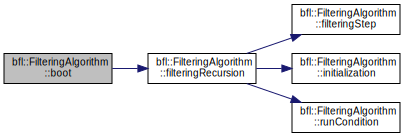
\includegraphics[width=350pt]{classbfl_1_1FilteringAlgorithm_a96651f8464190c0a56d79219a1017147_cgraph}
\end{center}
\end{figure}
\mbox{\Hypertarget{classbfl_1_1FilteringAlgorithm_ab3bceb43b5810a4bf1da884b8a0b145a}\label{classbfl_1_1FilteringAlgorithm_ab3bceb43b5810a4bf1da884b8a0b145a}} 
\index{bfl\+::\+Visual\+Particle\+Filter@{bfl\+::\+Visual\+Particle\+Filter}!filtering\+Step@{filtering\+Step}}
\index{filtering\+Step@{filtering\+Step}!bfl\+::\+Visual\+Particle\+Filter@{bfl\+::\+Visual\+Particle\+Filter}}
\subsubsection{\texorpdfstring{filtering\+Step()}{filteringStep()}}
{\footnotesize\ttfamily virtual void bfl\+::\+Filtering\+Algorithm\+::filtering\+Step (\begin{DoxyParamCaption}{ }\end{DoxyParamCaption})\hspace{0.3cm}{\ttfamily [protected]}, {\ttfamily [pure virtual]}, {\ttfamily [inherited]}}



Implemented in \mbox{\hyperlink{classbfl_1_1SIS_a582f06cc5456d2cc6ed8f90087cbbb4c}{bfl\+::\+S\+IS}}, \mbox{\hyperlink{classbfl_1_1UnscentedKalmanFilter_a169451bb711a03ad2dc28a40e3ad867f}{bfl\+::\+Unscented\+Kalman\+Filter}}, and \mbox{\hyperlink{classbfl_1_1KalmanFilter_aac6bd54422cba06e34cb93cb8a659950}{bfl\+::\+Kalman\+Filter}}.



Referenced by bfl\+::\+Filtering\+Algorithm\+::filtering\+Recursion().

\mbox{\Hypertarget{classbfl_1_1FilteringAlgorithm_a8c43b1f3dac30934c0a03de348d4a29d}\label{classbfl_1_1FilteringAlgorithm_a8c43b1f3dac30934c0a03de348d4a29d}} 
\index{bfl\+::\+Visual\+Particle\+Filter@{bfl\+::\+Visual\+Particle\+Filter}!get\+Filtering\+Step@{get\+Filtering\+Step}}
\index{get\+Filtering\+Step@{get\+Filtering\+Step}!bfl\+::\+Visual\+Particle\+Filter@{bfl\+::\+Visual\+Particle\+Filter}}
\subsubsection{\texorpdfstring{get\+Filtering\+Step()}{getFilteringStep()}}
{\footnotesize\ttfamily unsigned int Filtering\+Algorithm\+::get\+Filtering\+Step (\begin{DoxyParamCaption}{ }\end{DoxyParamCaption})\hspace{0.3cm}{\ttfamily [inherited]}}



Definition at line 86 of file Filtering\+Algorithm.\+cpp.



References bfl\+::\+Filtering\+Algorithm\+::filtering\+\_\+step\+\_\+.

\mbox{\Hypertarget{classbfl_1_1FilteringAlgorithm_acdfebf68405a427491e4dd9d020ae09b}\label{classbfl_1_1FilteringAlgorithm_acdfebf68405a427491e4dd9d020ae09b}} 
\index{bfl\+::\+Visual\+Particle\+Filter@{bfl\+::\+Visual\+Particle\+Filter}!get\+Result@{get\+Result}}
\index{get\+Result@{get\+Result}!bfl\+::\+Visual\+Particle\+Filter@{bfl\+::\+Visual\+Particle\+Filter}}
\subsubsection{\texorpdfstring{get\+Result()}{getResult()}}
{\footnotesize\ttfamily virtual void bfl\+::\+Filtering\+Algorithm\+::get\+Result (\begin{DoxyParamCaption}{ }\end{DoxyParamCaption})\hspace{0.3cm}{\ttfamily [protected]}, {\ttfamily [pure virtual]}, {\ttfamily [inherited]}}



Implemented in \mbox{\hyperlink{classbfl_1_1SIS_a059da4c932379643ff7005fe4d0fda89}{bfl\+::\+S\+IS}}, \mbox{\hyperlink{classbfl_1_1UnscentedKalmanFilter_ad25c4f9143bbe834b3adfc81c78b6743}{bfl\+::\+Unscented\+Kalman\+Filter}}, and \mbox{\hyperlink{classbfl_1_1KalmanFilter_a24484fb845495f43628db19062937548}{bfl\+::\+Kalman\+Filter}}.

\mbox{\Hypertarget{classbfl_1_1FilteringAlgorithm_af2a072aa51407fe5544bdbb7ce466e2a}\label{classbfl_1_1FilteringAlgorithm_af2a072aa51407fe5544bdbb7ce466e2a}} 
\index{bfl\+::\+Visual\+Particle\+Filter@{bfl\+::\+Visual\+Particle\+Filter}!initialization@{initialization}}
\index{initialization@{initialization}!bfl\+::\+Visual\+Particle\+Filter@{bfl\+::\+Visual\+Particle\+Filter}}
\subsubsection{\texorpdfstring{initialization()}{initialization()}}
{\footnotesize\ttfamily virtual void bfl\+::\+Filtering\+Algorithm\+::initialization (\begin{DoxyParamCaption}{ }\end{DoxyParamCaption})\hspace{0.3cm}{\ttfamily [protected]}, {\ttfamily [pure virtual]}, {\ttfamily [inherited]}}



Implemented in \mbox{\hyperlink{classbfl_1_1SIS_aaf9f4a14d51804eddcd93aa8a5ccbba8}{bfl\+::\+S\+IS}}, \mbox{\hyperlink{classbfl_1_1UnscentedKalmanFilter_acd5cfc6344d9ce24fb980aa22ecf4895}{bfl\+::\+Unscented\+Kalman\+Filter}}, and \mbox{\hyperlink{classbfl_1_1KalmanFilter_a34482fcfad20be0559cea9c060c5f949}{bfl\+::\+Kalman\+Filter}}.



Referenced by bfl\+::\+Filtering\+Algorithm\+::filtering\+Recursion(), set\+Initialization(), and bfl\+::\+Particle\+Filter\+::set\+Initialization().

\mbox{\Hypertarget{classbfl_1_1FilteringAlgorithm_a5cfecab2c778620e2557237472bb1721}\label{classbfl_1_1FilteringAlgorithm_a5cfecab2c778620e2557237472bb1721}} 
\index{bfl\+::\+Visual\+Particle\+Filter@{bfl\+::\+Visual\+Particle\+Filter}!is\+Running@{is\+Running}}
\index{is\+Running@{is\+Running}!bfl\+::\+Visual\+Particle\+Filter@{bfl\+::\+Visual\+Particle\+Filter}}
\subsubsection{\texorpdfstring{is\+Running()}{isRunning()}}
{\footnotesize\ttfamily bool Filtering\+Algorithm\+::is\+Running (\begin{DoxyParamCaption}{ }\end{DoxyParamCaption})\hspace{0.3cm}{\ttfamily [inherited]}}



Definition at line 92 of file Filtering\+Algorithm.\+cpp.



References bfl\+::\+Filtering\+Algorithm\+::run\+\_\+.

\mbox{\Hypertarget{classbfl_1_1VisualParticleFilter_a3044d7450e02d074207c61347b2c948f}\label{classbfl_1_1VisualParticleFilter_a3044d7450e02d074207c61347b2c948f}} 
\index{bfl\+::\+Visual\+Particle\+Filter@{bfl\+::\+Visual\+Particle\+Filter}!operator=@{operator=}}
\index{operator=@{operator=}!bfl\+::\+Visual\+Particle\+Filter@{bfl\+::\+Visual\+Particle\+Filter}}
\subsubsection{\texorpdfstring{operator=()}{operator=()}}
{\footnotesize\ttfamily \mbox{\hyperlink{classbfl_1_1VisualParticleFilter}{Visual\+Particle\+Filter}} \& Visual\+Particle\+Filter\+::operator= (\begin{DoxyParamCaption}\item[{\mbox{\hyperlink{classbfl_1_1VisualParticleFilter}{Visual\+Particle\+Filter}} \&\&}]{pf }\end{DoxyParamCaption})\hspace{0.3cm}{\ttfamily [protected]}, {\ttfamily [noexcept]}}



Definition at line 19 of file Visual\+Particle\+Filter.\+cpp.

\mbox{\Hypertarget{classbfl_1_1FilteringAlgorithm_a6022859aa985474fb997343cc935b11e}\label{classbfl_1_1FilteringAlgorithm_a6022859aa985474fb997343cc935b11e}} 
\index{bfl\+::\+Visual\+Particle\+Filter@{bfl\+::\+Visual\+Particle\+Filter}!reboot@{reboot}}
\index{reboot@{reboot}!bfl\+::\+Visual\+Particle\+Filter@{bfl\+::\+Visual\+Particle\+Filter}}
\subsubsection{\texorpdfstring{reboot()}{reboot()}}
{\footnotesize\ttfamily void Filtering\+Algorithm\+::reboot (\begin{DoxyParamCaption}{ }\end{DoxyParamCaption})\hspace{0.3cm}{\ttfamily [inherited]}}



Definition at line 66 of file Filtering\+Algorithm.\+cpp.



References bfl\+::\+Filtering\+Algorithm\+::cv\+\_\+run\+\_\+, bfl\+::\+Filtering\+Algorithm\+::mtx\+\_\+run\+\_\+, bfl\+::\+Filtering\+Algorithm\+::reset\+\_\+, and bfl\+::\+Filtering\+Algorithm\+::run\+\_\+.

\mbox{\Hypertarget{classbfl_1_1FilteringAlgorithm_a2403c62fbd7bd7f5cda56a84f5f30331}\label{classbfl_1_1FilteringAlgorithm_a2403c62fbd7bd7f5cda56a84f5f30331}} 
\index{bfl\+::\+Visual\+Particle\+Filter@{bfl\+::\+Visual\+Particle\+Filter}!reset@{reset}}
\index{reset@{reset}!bfl\+::\+Visual\+Particle\+Filter@{bfl\+::\+Visual\+Particle\+Filter}}
\subsubsection{\texorpdfstring{reset()}{reset()}}
{\footnotesize\ttfamily void Filtering\+Algorithm\+::reset (\begin{DoxyParamCaption}{ }\end{DoxyParamCaption})\hspace{0.3cm}{\ttfamily [inherited]}}



Definition at line 60 of file Filtering\+Algorithm.\+cpp.



References bfl\+::\+Filtering\+Algorithm\+::reset\+\_\+.

\mbox{\Hypertarget{classbfl_1_1FilteringAlgorithm_a009cbe5f4bbb16967f6c6ddcaed8fbb1}\label{classbfl_1_1FilteringAlgorithm_a009cbe5f4bbb16967f6c6ddcaed8fbb1}} 
\index{bfl\+::\+Visual\+Particle\+Filter@{bfl\+::\+Visual\+Particle\+Filter}!run@{run}}
\index{run@{run}!bfl\+::\+Visual\+Particle\+Filter@{bfl\+::\+Visual\+Particle\+Filter}}
\subsubsection{\texorpdfstring{run()}{run()}}
{\footnotesize\ttfamily void Filtering\+Algorithm\+::run (\begin{DoxyParamCaption}{ }\end{DoxyParamCaption})\hspace{0.3cm}{\ttfamily [inherited]}}



Definition at line 26 of file Filtering\+Algorithm.\+cpp.



References bfl\+::\+Filtering\+Algorithm\+::cv\+\_\+run\+\_\+, bfl\+::\+Filtering\+Algorithm\+::mtx\+\_\+run\+\_\+, and bfl\+::\+Filtering\+Algorithm\+::run\+\_\+.

\mbox{\Hypertarget{classbfl_1_1FilteringAlgorithm_a5fc12882356f6906b102fbfff2bc4b7c}\label{classbfl_1_1FilteringAlgorithm_a5fc12882356f6906b102fbfff2bc4b7c}} 
\index{bfl\+::\+Visual\+Particle\+Filter@{bfl\+::\+Visual\+Particle\+Filter}!run\+Condition@{run\+Condition}}
\index{run\+Condition@{run\+Condition}!bfl\+::\+Visual\+Particle\+Filter@{bfl\+::\+Visual\+Particle\+Filter}}
\subsubsection{\texorpdfstring{run\+Condition()}{runCondition()}}
{\footnotesize\ttfamily virtual bool bfl\+::\+Filtering\+Algorithm\+::run\+Condition (\begin{DoxyParamCaption}{ }\end{DoxyParamCaption})\hspace{0.3cm}{\ttfamily [protected]}, {\ttfamily [pure virtual]}, {\ttfamily [inherited]}}



Implemented in \mbox{\hyperlink{classbfl_1_1SIS_afb7cff1f7dae80e0e4ca84c925ca3ac3}{bfl\+::\+S\+IS}}.



Referenced by bfl\+::\+Filtering\+Algorithm\+::filtering\+Recursion().

\mbox{\Hypertarget{classbfl_1_1VisualParticleFilter_a77d03652f07d323b35aa478b0327b2f7}\label{classbfl_1_1VisualParticleFilter_a77d03652f07d323b35aa478b0327b2f7}} 
\index{bfl\+::\+Visual\+Particle\+Filter@{bfl\+::\+Visual\+Particle\+Filter}!set\+Correction@{set\+Correction}}
\index{set\+Correction@{set\+Correction}!bfl\+::\+Visual\+Particle\+Filter@{bfl\+::\+Visual\+Particle\+Filter}}
\subsubsection{\texorpdfstring{set\+Correction()}{setCorrection()}}
{\footnotesize\ttfamily void Visual\+Particle\+Filter\+::set\+Correction (\begin{DoxyParamCaption}\item[{std\+::unique\+\_\+ptr$<$ \mbox{\hyperlink{classbfl_1_1PFVisualCorrection}{P\+F\+Visual\+Correction}} $>$}]{correction }\end{DoxyParamCaption})}



Definition at line 42 of file Visual\+Particle\+Filter.\+cpp.



References correction\+\_\+.

\mbox{\Hypertarget{classbfl_1_1VisualParticleFilter_ac254d164f51ddbef8c79f8f1a7863a8d}\label{classbfl_1_1VisualParticleFilter_ac254d164f51ddbef8c79f8f1a7863a8d}} 
\index{bfl\+::\+Visual\+Particle\+Filter@{bfl\+::\+Visual\+Particle\+Filter}!set\+Initialization@{set\+Initialization}}
\index{set\+Initialization@{set\+Initialization}!bfl\+::\+Visual\+Particle\+Filter@{bfl\+::\+Visual\+Particle\+Filter}}
\subsubsection{\texorpdfstring{set\+Initialization()}{setInitialization()}}
{\footnotesize\ttfamily void Visual\+Particle\+Filter\+::set\+Initialization (\begin{DoxyParamCaption}\item[{std\+::unique\+\_\+ptr$<$ \mbox{\hyperlink{classbfl_1_1Initialization}{Initialization}} $>$}]{prediction }\end{DoxyParamCaption})}



Definition at line 30 of file Visual\+Particle\+Filter.\+cpp.



References bfl\+::\+Filtering\+Algorithm\+::initialization(), and initialization\+\_\+.

Here is the call graph for this function\+:
\nopagebreak
\begin{figure}[H]
\begin{center}
\leavevmode
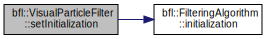
\includegraphics[width=338pt]{classbfl_1_1VisualParticleFilter_ac254d164f51ddbef8c79f8f1a7863a8d_cgraph}
\end{center}
\end{figure}
\mbox{\Hypertarget{classbfl_1_1VisualParticleFilter_addc3e844aa3fe41fb2241eb2215d0c63}\label{classbfl_1_1VisualParticleFilter_addc3e844aa3fe41fb2241eb2215d0c63}} 
\index{bfl\+::\+Visual\+Particle\+Filter@{bfl\+::\+Visual\+Particle\+Filter}!set\+Prediction@{set\+Prediction}}
\index{set\+Prediction@{set\+Prediction}!bfl\+::\+Visual\+Particle\+Filter@{bfl\+::\+Visual\+Particle\+Filter}}
\subsubsection{\texorpdfstring{set\+Prediction()}{setPrediction()}}
{\footnotesize\ttfamily void Visual\+Particle\+Filter\+::set\+Prediction (\begin{DoxyParamCaption}\item[{std\+::unique\+\_\+ptr$<$ \mbox{\hyperlink{classbfl_1_1PFPrediction}{P\+F\+Prediction}} $>$}]{prediction }\end{DoxyParamCaption})}



Definition at line 36 of file Visual\+Particle\+Filter.\+cpp.



References prediction\+\_\+.

\mbox{\Hypertarget{classbfl_1_1VisualParticleFilter_a4e42410d311df91ee14e31790ada3674}\label{classbfl_1_1VisualParticleFilter_a4e42410d311df91ee14e31790ada3674}} 
\index{bfl\+::\+Visual\+Particle\+Filter@{bfl\+::\+Visual\+Particle\+Filter}!set\+Resampling@{set\+Resampling}}
\index{set\+Resampling@{set\+Resampling}!bfl\+::\+Visual\+Particle\+Filter@{bfl\+::\+Visual\+Particle\+Filter}}
\subsubsection{\texorpdfstring{set\+Resampling()}{setResampling()}}
{\footnotesize\ttfamily void Visual\+Particle\+Filter\+::set\+Resampling (\begin{DoxyParamCaption}\item[{std\+::unique\+\_\+ptr$<$ \mbox{\hyperlink{classbfl_1_1Resampling}{Resampling}} $>$}]{resampling }\end{DoxyParamCaption})}



Definition at line 48 of file Visual\+Particle\+Filter.\+cpp.



References resampling\+\_\+.

\mbox{\Hypertarget{classbfl_1_1VisualParticleFilter_aab68e455c645bc1b7b8c3c2b476c2f9c}\label{classbfl_1_1VisualParticleFilter_aab68e455c645bc1b7b8c3c2b476c2f9c}} 
\index{bfl\+::\+Visual\+Particle\+Filter@{bfl\+::\+Visual\+Particle\+Filter}!skip@{skip}}
\index{skip@{skip}!bfl\+::\+Visual\+Particle\+Filter@{bfl\+::\+Visual\+Particle\+Filter}}
\subsubsection{\texorpdfstring{skip()}{skip()}}
{\footnotesize\ttfamily bool Visual\+Particle\+Filter\+::skip (\begin{DoxyParamCaption}\item[{const std\+::string \&}]{what\+\_\+step,  }\item[{const bool}]{status }\end{DoxyParamCaption})\hspace{0.3cm}{\ttfamily [override]}, {\ttfamily [virtual]}}



Implements \mbox{\hyperlink{classbfl_1_1FilteringAlgorithm_ac8a718a614905d89d6a43bbbc70d68b2}{bfl\+::\+Filtering\+Algorithm}}.



Definition at line 54 of file Visual\+Particle\+Filter.\+cpp.



References correction\+\_\+, and prediction\+\_\+.

\mbox{\Hypertarget{classbfl_1_1FilteringAlgorithm_a1dc912d89ee8f96d4f3e8209865c5308}\label{classbfl_1_1FilteringAlgorithm_a1dc912d89ee8f96d4f3e8209865c5308}} 
\index{bfl\+::\+Visual\+Particle\+Filter@{bfl\+::\+Visual\+Particle\+Filter}!teardown@{teardown}}
\index{teardown@{teardown}!bfl\+::\+Visual\+Particle\+Filter@{bfl\+::\+Visual\+Particle\+Filter}}
\subsubsection{\texorpdfstring{teardown()}{teardown()}}
{\footnotesize\ttfamily bool Filtering\+Algorithm\+::teardown (\begin{DoxyParamCaption}{ }\end{DoxyParamCaption})\hspace{0.3cm}{\ttfamily [inherited]}}



Definition at line 75 of file Filtering\+Algorithm.\+cpp.



References bfl\+::\+Filtering\+Algorithm\+::teardown\+\_\+.

\mbox{\Hypertarget{classbfl_1_1FilteringAlgorithm_a40372c24fa050eb0274371172df0a244}\label{classbfl_1_1FilteringAlgorithm_a40372c24fa050eb0274371172df0a244}} 
\index{bfl\+::\+Visual\+Particle\+Filter@{bfl\+::\+Visual\+Particle\+Filter}!wait@{wait}}
\index{wait@{wait}!bfl\+::\+Visual\+Particle\+Filter@{bfl\+::\+Visual\+Particle\+Filter}}
\subsubsection{\texorpdfstring{wait()}{wait()}}
{\footnotesize\ttfamily bool Filtering\+Algorithm\+::wait (\begin{DoxyParamCaption}{ }\end{DoxyParamCaption})\hspace{0.3cm}{\ttfamily [inherited]}}



Definition at line 34 of file Filtering\+Algorithm.\+cpp.



References bfl\+::\+Filtering\+Algorithm\+::filtering\+\_\+thread\+\_\+.



\subsection{Member Data Documentation}
\mbox{\Hypertarget{classbfl_1_1VisualParticleFilter_af267eeba1c05e0961545ec9c4efc0bbf}\label{classbfl_1_1VisualParticleFilter_af267eeba1c05e0961545ec9c4efc0bbf}} 
\index{bfl\+::\+Visual\+Particle\+Filter@{bfl\+::\+Visual\+Particle\+Filter}!correction\+\_\+@{correction\+\_\+}}
\index{correction\+\_\+@{correction\+\_\+}!bfl\+::\+Visual\+Particle\+Filter@{bfl\+::\+Visual\+Particle\+Filter}}
\subsubsection{\texorpdfstring{correction\+\_\+}{correction\_}}
{\footnotesize\ttfamily std\+::unique\+\_\+ptr$<$\mbox{\hyperlink{classbfl_1_1PFVisualCorrection}{P\+F\+Visual\+Correction}}$>$ bfl\+::\+Visual\+Particle\+Filter\+::correction\+\_\+\hspace{0.3cm}{\ttfamily [protected]}}



Definition at line 41 of file Visual\+Particle\+Filter.\+h.



Referenced by set\+Correction(), and skip().

\mbox{\Hypertarget{classbfl_1_1VisualParticleFilter_abe1c7110a109cd18adc923e23179f531}\label{classbfl_1_1VisualParticleFilter_abe1c7110a109cd18adc923e23179f531}} 
\index{bfl\+::\+Visual\+Particle\+Filter@{bfl\+::\+Visual\+Particle\+Filter}!initialization\+\_\+@{initialization\+\_\+}}
\index{initialization\+\_\+@{initialization\+\_\+}!bfl\+::\+Visual\+Particle\+Filter@{bfl\+::\+Visual\+Particle\+Filter}}
\subsubsection{\texorpdfstring{initialization\+\_\+}{initialization\_}}
{\footnotesize\ttfamily std\+::unique\+\_\+ptr$<$\mbox{\hyperlink{classbfl_1_1Initialization}{Initialization}}$>$ bfl\+::\+Visual\+Particle\+Filter\+::initialization\+\_\+\hspace{0.3cm}{\ttfamily [protected]}}



Definition at line 39 of file Visual\+Particle\+Filter.\+h.



Referenced by set\+Initialization().

\mbox{\Hypertarget{classbfl_1_1VisualParticleFilter_a3c2ffe1f100e4fb4979922fa76b41494}\label{classbfl_1_1VisualParticleFilter_a3c2ffe1f100e4fb4979922fa76b41494}} 
\index{bfl\+::\+Visual\+Particle\+Filter@{bfl\+::\+Visual\+Particle\+Filter}!prediction\+\_\+@{prediction\+\_\+}}
\index{prediction\+\_\+@{prediction\+\_\+}!bfl\+::\+Visual\+Particle\+Filter@{bfl\+::\+Visual\+Particle\+Filter}}
\subsubsection{\texorpdfstring{prediction\+\_\+}{prediction\_}}
{\footnotesize\ttfamily std\+::unique\+\_\+ptr$<$\mbox{\hyperlink{classbfl_1_1PFPrediction}{P\+F\+Prediction}}$>$ bfl\+::\+Visual\+Particle\+Filter\+::prediction\+\_\+\hspace{0.3cm}{\ttfamily [protected]}}



Definition at line 40 of file Visual\+Particle\+Filter.\+h.



Referenced by set\+Prediction(), and skip().

\mbox{\Hypertarget{classbfl_1_1VisualParticleFilter_aa0b7a55de5ccd0ffb6ebdf765bf73e07}\label{classbfl_1_1VisualParticleFilter_aa0b7a55de5ccd0ffb6ebdf765bf73e07}} 
\index{bfl\+::\+Visual\+Particle\+Filter@{bfl\+::\+Visual\+Particle\+Filter}!resampling\+\_\+@{resampling\+\_\+}}
\index{resampling\+\_\+@{resampling\+\_\+}!bfl\+::\+Visual\+Particle\+Filter@{bfl\+::\+Visual\+Particle\+Filter}}
\subsubsection{\texorpdfstring{resampling\+\_\+}{resampling\_}}
{\footnotesize\ttfamily std\+::unique\+\_\+ptr$<$\mbox{\hyperlink{classbfl_1_1Resampling}{Resampling}}$>$ bfl\+::\+Visual\+Particle\+Filter\+::resampling\+\_\+\hspace{0.3cm}{\ttfamily [protected]}}



Definition at line 42 of file Visual\+Particle\+Filter.\+h.



Referenced by set\+Resampling().



The documentation for this class was generated from the following files\+:\begin{DoxyCompactItemize}
\item 
C\+:/\+Users/cfantacci/\+Git\+Hub/bayes-\/filters-\/lib/src/\+Bayes\+Filters/include/\+Bayes\+Filters/\mbox{\hyperlink{VisualParticleFilter_8h}{Visual\+Particle\+Filter.\+h}}\item 
C\+:/\+Users/cfantacci/\+Git\+Hub/bayes-\/filters-\/lib/src/\+Bayes\+Filters/src/\mbox{\hyperlink{VisualParticleFilter_8cpp}{Visual\+Particle\+Filter.\+cpp}}\end{DoxyCompactItemize}

\hypertarget{classbfl_1_1WhiteNoiseAcceleration}{}\section{bfl\+:\+:White\+Noise\+Acceleration Class Reference}
\label{classbfl_1_1WhiteNoiseAcceleration}\index{bfl\+::\+White\+Noise\+Acceleration@{bfl\+::\+White\+Noise\+Acceleration}}


{\ttfamily \#include $<$White\+Noise\+Acceleration.\+h$>$}



Inheritance diagram for bfl\+:\+:White\+Noise\+Acceleration\+:
\nopagebreak
\begin{figure}[H]
\begin{center}
\leavevmode
\includegraphics[width=217pt]{classbfl_1_1WhiteNoiseAcceleration__inherit__graph}
\end{center}
\end{figure}
\subsection*{Public Member Functions}
\begin{DoxyCompactItemize}
\item 
\mbox{\hyperlink{classbfl_1_1WhiteNoiseAcceleration_a5eb5d6b767ad37ecc93e0ce1dd944e8a}{White\+Noise\+Acceleration}} (float T, float tilde\+\_\+q, unsigned int seed) noexcept
\item 
\mbox{\hyperlink{classbfl_1_1WhiteNoiseAcceleration_a689e238bdbd0ccaf488e8a1c9e897825}{White\+Noise\+Acceleration}} (float T, float tilde\+\_\+q) noexcept
\item 
\mbox{\hyperlink{classbfl_1_1WhiteNoiseAcceleration_aae68b94c0d82a6fa594e0e1feba7e272}{White\+Noise\+Acceleration}} () noexcept
\item 
\mbox{\hyperlink{classbfl_1_1WhiteNoiseAcceleration_ac01e4702a8fbce92a7fd0adf74472e5a}{White\+Noise\+Acceleration}} (const \mbox{\hyperlink{classbfl_1_1WhiteNoiseAcceleration}{White\+Noise\+Acceleration}} \&wna)
\item 
\mbox{\hyperlink{classbfl_1_1WhiteNoiseAcceleration_a74f0f6d44c76e10627765d405de96af6}{White\+Noise\+Acceleration}} (\mbox{\hyperlink{classbfl_1_1WhiteNoiseAcceleration}{White\+Noise\+Acceleration}} \&\&wna) noexcept
\item 
virtual \mbox{\hyperlink{classbfl_1_1WhiteNoiseAcceleration_a17d13fe4ece8cb6db9f2423ff48f817d}{$\sim$\+White\+Noise\+Acceleration}} () noexcept
\item 
\mbox{\hyperlink{classbfl_1_1WhiteNoiseAcceleration}{White\+Noise\+Acceleration}} \& \mbox{\hyperlink{classbfl_1_1WhiteNoiseAcceleration_a6f69d09499e7a4746bd823db5fc5ceec}{operator=}} (const \mbox{\hyperlink{classbfl_1_1WhiteNoiseAcceleration}{White\+Noise\+Acceleration}} \&wna)
\item 
\mbox{\hyperlink{classbfl_1_1WhiteNoiseAcceleration}{White\+Noise\+Acceleration}} \& \mbox{\hyperlink{classbfl_1_1WhiteNoiseAcceleration_a4562a1dfc45dd143f7d05fea98e38f42}{operator=}} (\mbox{\hyperlink{classbfl_1_1WhiteNoiseAcceleration}{White\+Noise\+Acceleration}} \&\&wna) noexcept
\item 
void \mbox{\hyperlink{classbfl_1_1WhiteNoiseAcceleration_a1c2f938f535c20c78447a69c76c6896b}{propagate}} (const Eigen\+::\+Ref$<$ const Eigen\+::\+Matrix\+Xf $>$ \&cur\+\_\+states, Eigen\+::\+Ref$<$ Eigen\+::\+Matrix\+Xf $>$ prop\+\_\+states) override
\item 
void \mbox{\hyperlink{classbfl_1_1WhiteNoiseAcceleration_addb79c08bdf08b89629bdcd24e46d1b8}{motion}} (const Eigen\+::\+Ref$<$ const Eigen\+::\+Matrix\+Xf $>$ \&cur\+\_\+states, Eigen\+::\+Ref$<$ Eigen\+::\+Matrix\+Xf $>$ prop\+\_\+states) override
\item 
Eigen\+::\+Matrix\+Xf \mbox{\hyperlink{classbfl_1_1WhiteNoiseAcceleration_ac4bf4116d3a88435b9d070cbc8736656}{get\+Noise\+Sample}} (const int num) override
\item 
Eigen\+::\+Matrix\+Xf \mbox{\hyperlink{classbfl_1_1WhiteNoiseAcceleration_a09c79104b153e6fb610bb2f1c6405636}{get\+Noise\+Covariance\+Matrix}} () override
\item 
bool \mbox{\hyperlink{classbfl_1_1WhiteNoiseAcceleration_a0203b47074e0680852f53dcba8a7a627}{set\+Property}} (const std\+::string \&property) override
\end{DoxyCompactItemize}
\subsection*{Protected Attributes}
\begin{DoxyCompactItemize}
\item 
float \mbox{\hyperlink{classbfl_1_1WhiteNoiseAcceleration_a7d1674033e2b6b1b8f245e910163aa0a}{T\+\_\+}}
\item 
Eigen\+::\+Matrix4f \mbox{\hyperlink{classbfl_1_1WhiteNoiseAcceleration_a02c209c5ca35170a096fc4ebe6754193}{F\+\_\+}}
\item 
Eigen\+::\+Matrix4f \mbox{\hyperlink{classbfl_1_1WhiteNoiseAcceleration_ad65c6f3766d7dd6d4b01bd84c3f0862d}{Q\+\_\+}}
\item 
float \mbox{\hyperlink{classbfl_1_1WhiteNoiseAcceleration_a5025cf01732a8ed99f4057fa6726f03e}{tilde\+\_\+q\+\_\+}}
\item 
Eigen\+::\+Matrix4f \mbox{\hyperlink{classbfl_1_1WhiteNoiseAcceleration_a209890197d296e25b22f0a04eec9bb0b}{sqrt\+\_\+\+Q\+\_\+}}
\item 
std\+::mt19937\+\_\+64 \mbox{\hyperlink{classbfl_1_1WhiteNoiseAcceleration_a53532f567190af8a0baa579e3bd4e362}{generator\+\_\+}}
\item 
std\+::normal\+\_\+distribution$<$ float $>$ \mbox{\hyperlink{classbfl_1_1WhiteNoiseAcceleration_ad6d1649c319820d8f7cc9eb65666542f}{distribution\+\_\+}}
\item 
std\+::function$<$ float()$>$ \mbox{\hyperlink{classbfl_1_1WhiteNoiseAcceleration_a18feb2398836b38928e8e9fe367d5ab6}{gauss\+\_\+rnd\+\_\+sample\+\_\+}}
\end{DoxyCompactItemize}


\subsection{Detailed Description}


Definition at line 14 of file White\+Noise\+Acceleration.\+h.



\subsection{Constructor \& Destructor Documentation}
\mbox{\Hypertarget{classbfl_1_1WhiteNoiseAcceleration_a5eb5d6b767ad37ecc93e0ce1dd944e8a}\label{classbfl_1_1WhiteNoiseAcceleration_a5eb5d6b767ad37ecc93e0ce1dd944e8a}} 
\index{bfl\+::\+White\+Noise\+Acceleration@{bfl\+::\+White\+Noise\+Acceleration}!White\+Noise\+Acceleration@{White\+Noise\+Acceleration}}
\index{White\+Noise\+Acceleration@{White\+Noise\+Acceleration}!bfl\+::\+White\+Noise\+Acceleration@{bfl\+::\+White\+Noise\+Acceleration}}
\subsubsection{\texorpdfstring{White\+Noise\+Acceleration()}{WhiteNoiseAcceleration()}\hspace{0.1cm}{\footnotesize\ttfamily [1/5]}}
{\footnotesize\ttfamily White\+Noise\+Acceleration\+::\+White\+Noise\+Acceleration (\begin{DoxyParamCaption}\item[{float}]{T,  }\item[{float}]{tilde\+\_\+q,  }\item[{unsigned int}]{seed }\end{DoxyParamCaption})\hspace{0.3cm}{\ttfamily [noexcept]}}



Definition at line 12 of file White\+Noise\+Acceleration.\+cpp.

\mbox{\Hypertarget{classbfl_1_1WhiteNoiseAcceleration_a689e238bdbd0ccaf488e8a1c9e897825}\label{classbfl_1_1WhiteNoiseAcceleration_a689e238bdbd0ccaf488e8a1c9e897825}} 
\index{bfl\+::\+White\+Noise\+Acceleration@{bfl\+::\+White\+Noise\+Acceleration}!White\+Noise\+Acceleration@{White\+Noise\+Acceleration}}
\index{White\+Noise\+Acceleration@{White\+Noise\+Acceleration}!bfl\+::\+White\+Noise\+Acceleration@{bfl\+::\+White\+Noise\+Acceleration}}
\subsubsection{\texorpdfstring{White\+Noise\+Acceleration()}{WhiteNoiseAcceleration()}\hspace{0.1cm}{\footnotesize\ttfamily [2/5]}}
{\footnotesize\ttfamily White\+Noise\+Acceleration\+::\+White\+Noise\+Acceleration (\begin{DoxyParamCaption}\item[{float}]{T,  }\item[{float}]{tilde\+\_\+q }\end{DoxyParamCaption})\hspace{0.3cm}{\ttfamily [noexcept]}}



Definition at line 34 of file White\+Noise\+Acceleration.\+cpp.

\mbox{\Hypertarget{classbfl_1_1WhiteNoiseAcceleration_aae68b94c0d82a6fa594e0e1feba7e272}\label{classbfl_1_1WhiteNoiseAcceleration_aae68b94c0d82a6fa594e0e1feba7e272}} 
\index{bfl\+::\+White\+Noise\+Acceleration@{bfl\+::\+White\+Noise\+Acceleration}!White\+Noise\+Acceleration@{White\+Noise\+Acceleration}}
\index{White\+Noise\+Acceleration@{White\+Noise\+Acceleration}!bfl\+::\+White\+Noise\+Acceleration@{bfl\+::\+White\+Noise\+Acceleration}}
\subsubsection{\texorpdfstring{White\+Noise\+Acceleration()}{WhiteNoiseAcceleration()}\hspace{0.1cm}{\footnotesize\ttfamily [3/5]}}
{\footnotesize\ttfamily White\+Noise\+Acceleration\+::\+White\+Noise\+Acceleration (\begin{DoxyParamCaption}{ }\end{DoxyParamCaption})\hspace{0.3cm}{\ttfamily [noexcept]}}



Definition at line 38 of file White\+Noise\+Acceleration.\+cpp.

\mbox{\Hypertarget{classbfl_1_1WhiteNoiseAcceleration_ac01e4702a8fbce92a7fd0adf74472e5a}\label{classbfl_1_1WhiteNoiseAcceleration_ac01e4702a8fbce92a7fd0adf74472e5a}} 
\index{bfl\+::\+White\+Noise\+Acceleration@{bfl\+::\+White\+Noise\+Acceleration}!White\+Noise\+Acceleration@{White\+Noise\+Acceleration}}
\index{White\+Noise\+Acceleration@{White\+Noise\+Acceleration}!bfl\+::\+White\+Noise\+Acceleration@{bfl\+::\+White\+Noise\+Acceleration}}
\subsubsection{\texorpdfstring{White\+Noise\+Acceleration()}{WhiteNoiseAcceleration()}\hspace{0.1cm}{\footnotesize\ttfamily [4/5]}}
{\footnotesize\ttfamily White\+Noise\+Acceleration\+::\+White\+Noise\+Acceleration (\begin{DoxyParamCaption}\item[{const \mbox{\hyperlink{classbfl_1_1WhiteNoiseAcceleration}{White\+Noise\+Acceleration}} \&}]{wna }\end{DoxyParamCaption})}



Definition at line 45 of file White\+Noise\+Acceleration.\+cpp.

\mbox{\Hypertarget{classbfl_1_1WhiteNoiseAcceleration_a74f0f6d44c76e10627765d405de96af6}\label{classbfl_1_1WhiteNoiseAcceleration_a74f0f6d44c76e10627765d405de96af6}} 
\index{bfl\+::\+White\+Noise\+Acceleration@{bfl\+::\+White\+Noise\+Acceleration}!White\+Noise\+Acceleration@{White\+Noise\+Acceleration}}
\index{White\+Noise\+Acceleration@{White\+Noise\+Acceleration}!bfl\+::\+White\+Noise\+Acceleration@{bfl\+::\+White\+Noise\+Acceleration}}
\subsubsection{\texorpdfstring{White\+Noise\+Acceleration()}{WhiteNoiseAcceleration()}\hspace{0.1cm}{\footnotesize\ttfamily [5/5]}}
{\footnotesize\ttfamily White\+Noise\+Acceleration\+::\+White\+Noise\+Acceleration (\begin{DoxyParamCaption}\item[{\mbox{\hyperlink{classbfl_1_1WhiteNoiseAcceleration}{White\+Noise\+Acceleration}} \&\&}]{wna }\end{DoxyParamCaption})\hspace{0.3cm}{\ttfamily [noexcept]}}



Definition at line 50 of file White\+Noise\+Acceleration.\+cpp.

\mbox{\Hypertarget{classbfl_1_1WhiteNoiseAcceleration_a17d13fe4ece8cb6db9f2423ff48f817d}\label{classbfl_1_1WhiteNoiseAcceleration_a17d13fe4ece8cb6db9f2423ff48f817d}} 
\index{bfl\+::\+White\+Noise\+Acceleration@{bfl\+::\+White\+Noise\+Acceleration}!````~White\+Noise\+Acceleration@{$\sim$\+White\+Noise\+Acceleration}}
\index{````~White\+Noise\+Acceleration@{$\sim$\+White\+Noise\+Acceleration}!bfl\+::\+White\+Noise\+Acceleration@{bfl\+::\+White\+Noise\+Acceleration}}
\subsubsection{\texorpdfstring{$\sim$\+White\+Noise\+Acceleration()}{~WhiteNoiseAcceleration()}}
{\footnotesize\ttfamily White\+Noise\+Acceleration\+::$\sim$\+White\+Noise\+Acceleration (\begin{DoxyParamCaption}{ }\end{DoxyParamCaption})\hspace{0.3cm}{\ttfamily [virtual]}, {\ttfamily [noexcept]}}



Definition at line 42 of file White\+Noise\+Acceleration.\+cpp.



\subsection{Member Function Documentation}
\mbox{\Hypertarget{classbfl_1_1WhiteNoiseAcceleration_a09c79104b153e6fb610bb2f1c6405636}\label{classbfl_1_1WhiteNoiseAcceleration_a09c79104b153e6fb610bb2f1c6405636}} 
\index{bfl\+::\+White\+Noise\+Acceleration@{bfl\+::\+White\+Noise\+Acceleration}!get\+Noise\+Covariance\+Matrix@{get\+Noise\+Covariance\+Matrix}}
\index{get\+Noise\+Covariance\+Matrix@{get\+Noise\+Covariance\+Matrix}!bfl\+::\+White\+Noise\+Acceleration@{bfl\+::\+White\+Noise\+Acceleration}}
\subsubsection{\texorpdfstring{get\+Noise\+Covariance\+Matrix()}{getNoiseCovarianceMatrix()}}
{\footnotesize\ttfamily Matrix\+Xf White\+Noise\+Acceleration\+::get\+Noise\+Covariance\+Matrix (\begin{DoxyParamCaption}{ }\end{DoxyParamCaption})\hspace{0.3cm}{\ttfamily [override]}, {\ttfamily [virtual]}}



Implements \mbox{\hyperlink{classbfl_1_1StateModel_a606efee8bf37606833c1ac75f2fbb357}{bfl\+::\+State\+Model}}.



Definition at line 111 of file White\+Noise\+Acceleration.\+cpp.



References Q\+\_\+.

\mbox{\Hypertarget{classbfl_1_1WhiteNoiseAcceleration_ac4bf4116d3a88435b9d070cbc8736656}\label{classbfl_1_1WhiteNoiseAcceleration_ac4bf4116d3a88435b9d070cbc8736656}} 
\index{bfl\+::\+White\+Noise\+Acceleration@{bfl\+::\+White\+Noise\+Acceleration}!get\+Noise\+Sample@{get\+Noise\+Sample}}
\index{get\+Noise\+Sample@{get\+Noise\+Sample}!bfl\+::\+White\+Noise\+Acceleration@{bfl\+::\+White\+Noise\+Acceleration}}
\subsubsection{\texorpdfstring{get\+Noise\+Sample()}{getNoiseSample()}}
{\footnotesize\ttfamily Matrix\+Xf White\+Noise\+Acceleration\+::get\+Noise\+Sample (\begin{DoxyParamCaption}\item[{const int}]{num }\end{DoxyParamCaption})\hspace{0.3cm}{\ttfamily [override]}, {\ttfamily [virtual]}}



Implements \mbox{\hyperlink{classbfl_1_1StateModel_ab1f0aa4c804b7de86c68294de3df76ee}{bfl\+::\+State\+Model}}.



Definition at line 101 of file White\+Noise\+Acceleration.\+cpp.



References gauss\+\_\+rnd\+\_\+sample\+\_\+, and sqrt\+\_\+\+Q\+\_\+.



Referenced by motion().

\mbox{\Hypertarget{classbfl_1_1WhiteNoiseAcceleration_addb79c08bdf08b89629bdcd24e46d1b8}\label{classbfl_1_1WhiteNoiseAcceleration_addb79c08bdf08b89629bdcd24e46d1b8}} 
\index{bfl\+::\+White\+Noise\+Acceleration@{bfl\+::\+White\+Noise\+Acceleration}!motion@{motion}}
\index{motion@{motion}!bfl\+::\+White\+Noise\+Acceleration@{bfl\+::\+White\+Noise\+Acceleration}}
\subsubsection{\texorpdfstring{motion()}{motion()}}
{\footnotesize\ttfamily void White\+Noise\+Acceleration\+::motion (\begin{DoxyParamCaption}\item[{const Eigen\+::\+Ref$<$ const Eigen\+::\+Matrix\+Xf $>$ \&}]{cur\+\_\+states,  }\item[{Eigen\+::\+Ref$<$ Eigen\+::\+Matrix\+Xf $>$}]{prop\+\_\+states }\end{DoxyParamCaption})\hspace{0.3cm}{\ttfamily [override]}, {\ttfamily [virtual]}}



Implements \mbox{\hyperlink{classbfl_1_1StateModel_a3601485697ae3445ec7ca753dbeb035c}{bfl\+::\+State\+Model}}.



Definition at line 93 of file White\+Noise\+Acceleration.\+cpp.



References get\+Noise\+Sample(), and propagate().

Here is the call graph for this function\+:
\nopagebreak
\begin{figure}[H]
\begin{center}
\leavevmode
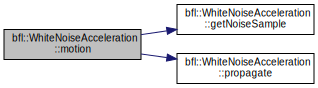
\includegraphics[width=350pt]{classbfl_1_1WhiteNoiseAcceleration_addb79c08bdf08b89629bdcd24e46d1b8_cgraph}
\end{center}
\end{figure}
\mbox{\Hypertarget{classbfl_1_1WhiteNoiseAcceleration_a6f69d09499e7a4746bd823db5fc5ceec}\label{classbfl_1_1WhiteNoiseAcceleration_a6f69d09499e7a4746bd823db5fc5ceec}} 
\index{bfl\+::\+White\+Noise\+Acceleration@{bfl\+::\+White\+Noise\+Acceleration}!operator=@{operator=}}
\index{operator=@{operator=}!bfl\+::\+White\+Noise\+Acceleration@{bfl\+::\+White\+Noise\+Acceleration}}
\subsubsection{\texorpdfstring{operator=()}{operator=()}\hspace{0.1cm}{\footnotesize\ttfamily [1/2]}}
{\footnotesize\ttfamily \mbox{\hyperlink{classbfl_1_1WhiteNoiseAcceleration}{White\+Noise\+Acceleration}} \& White\+Noise\+Acceleration\+::operator= (\begin{DoxyParamCaption}\item[{const \mbox{\hyperlink{classbfl_1_1WhiteNoiseAcceleration}{White\+Noise\+Acceleration}} \&}]{wna }\end{DoxyParamCaption})}



Definition at line 59 of file White\+Noise\+Acceleration.\+cpp.

\mbox{\Hypertarget{classbfl_1_1WhiteNoiseAcceleration_a4562a1dfc45dd143f7d05fea98e38f42}\label{classbfl_1_1WhiteNoiseAcceleration_a4562a1dfc45dd143f7d05fea98e38f42}} 
\index{bfl\+::\+White\+Noise\+Acceleration@{bfl\+::\+White\+Noise\+Acceleration}!operator=@{operator=}}
\index{operator=@{operator=}!bfl\+::\+White\+Noise\+Acceleration@{bfl\+::\+White\+Noise\+Acceleration}}
\subsubsection{\texorpdfstring{operator=()}{operator=()}\hspace{0.1cm}{\footnotesize\ttfamily [2/2]}}
{\footnotesize\ttfamily \mbox{\hyperlink{classbfl_1_1WhiteNoiseAcceleration}{White\+Noise\+Acceleration}} \& White\+Noise\+Acceleration\+::operator= (\begin{DoxyParamCaption}\item[{\mbox{\hyperlink{classbfl_1_1WhiteNoiseAcceleration}{White\+Noise\+Acceleration}} \&\&}]{wna }\end{DoxyParamCaption})\hspace{0.3cm}{\ttfamily [noexcept]}}



Definition at line 68 of file White\+Noise\+Acceleration.\+cpp.



References T\+\_\+.

\mbox{\Hypertarget{classbfl_1_1WhiteNoiseAcceleration_a1c2f938f535c20c78447a69c76c6896b}\label{classbfl_1_1WhiteNoiseAcceleration_a1c2f938f535c20c78447a69c76c6896b}} 
\index{bfl\+::\+White\+Noise\+Acceleration@{bfl\+::\+White\+Noise\+Acceleration}!propagate@{propagate}}
\index{propagate@{propagate}!bfl\+::\+White\+Noise\+Acceleration@{bfl\+::\+White\+Noise\+Acceleration}}
\subsubsection{\texorpdfstring{propagate()}{propagate()}}
{\footnotesize\ttfamily void White\+Noise\+Acceleration\+::propagate (\begin{DoxyParamCaption}\item[{const Eigen\+::\+Ref$<$ const Eigen\+::\+Matrix\+Xf $>$ \&}]{cur\+\_\+states,  }\item[{Eigen\+::\+Ref$<$ Eigen\+::\+Matrix\+Xf $>$}]{prop\+\_\+states }\end{DoxyParamCaption})\hspace{0.3cm}{\ttfamily [override]}, {\ttfamily [virtual]}}



Implements \mbox{\hyperlink{classbfl_1_1StateModel_a47a625abb7df9b7afa689ccb9aa11aee}{bfl\+::\+State\+Model}}.



Definition at line 87 of file White\+Noise\+Acceleration.\+cpp.



References F\+\_\+.



Referenced by motion().

\mbox{\Hypertarget{classbfl_1_1WhiteNoiseAcceleration_a0203b47074e0680852f53dcba8a7a627}\label{classbfl_1_1WhiteNoiseAcceleration_a0203b47074e0680852f53dcba8a7a627}} 
\index{bfl\+::\+White\+Noise\+Acceleration@{bfl\+::\+White\+Noise\+Acceleration}!set\+Property@{set\+Property}}
\index{set\+Property@{set\+Property}!bfl\+::\+White\+Noise\+Acceleration@{bfl\+::\+White\+Noise\+Acceleration}}
\subsubsection{\texorpdfstring{set\+Property()}{setProperty()}}
{\footnotesize\ttfamily bool bfl\+::\+White\+Noise\+Acceleration\+::set\+Property (\begin{DoxyParamCaption}\item[{const std\+::string \&}]{property }\end{DoxyParamCaption})\hspace{0.3cm}{\ttfamily [inline]}, {\ttfamily [override]}, {\ttfamily [virtual]}}



Implements \mbox{\hyperlink{classbfl_1_1StateModel_ac86dcdad8f0bbfab39a23e592779feaa}{bfl\+::\+State\+Model}}.



Definition at line 41 of file White\+Noise\+Acceleration.\+h.



\subsection{Member Data Documentation}
\mbox{\Hypertarget{classbfl_1_1WhiteNoiseAcceleration_ad6d1649c319820d8f7cc9eb65666542f}\label{classbfl_1_1WhiteNoiseAcceleration_ad6d1649c319820d8f7cc9eb65666542f}} 
\index{bfl\+::\+White\+Noise\+Acceleration@{bfl\+::\+White\+Noise\+Acceleration}!distribution\+\_\+@{distribution\+\_\+}}
\index{distribution\+\_\+@{distribution\+\_\+}!bfl\+::\+White\+Noise\+Acceleration@{bfl\+::\+White\+Noise\+Acceleration}}
\subsubsection{\texorpdfstring{distribution\+\_\+}{distribution\_}}
{\footnotesize\ttfamily std\+::normal\+\_\+distribution$<$float$>$ bfl\+::\+White\+Noise\+Acceleration\+::distribution\+\_\+\hspace{0.3cm}{\ttfamily [protected]}}



Definition at line 51 of file White\+Noise\+Acceleration.\+h.

\mbox{\Hypertarget{classbfl_1_1WhiteNoiseAcceleration_a02c209c5ca35170a096fc4ebe6754193}\label{classbfl_1_1WhiteNoiseAcceleration_a02c209c5ca35170a096fc4ebe6754193}} 
\index{bfl\+::\+White\+Noise\+Acceleration@{bfl\+::\+White\+Noise\+Acceleration}!F\+\_\+@{F\+\_\+}}
\index{F\+\_\+@{F\+\_\+}!bfl\+::\+White\+Noise\+Acceleration@{bfl\+::\+White\+Noise\+Acceleration}}
\subsubsection{\texorpdfstring{F\+\_\+}{F\_}}
{\footnotesize\ttfamily Eigen\+::\+Matrix4f bfl\+::\+White\+Noise\+Acceleration\+::\+F\+\_\+\hspace{0.3cm}{\ttfamily [protected]}}



Definition at line 45 of file White\+Noise\+Acceleration.\+h.



Referenced by propagate().

\mbox{\Hypertarget{classbfl_1_1WhiteNoiseAcceleration_a18feb2398836b38928e8e9fe367d5ab6}\label{classbfl_1_1WhiteNoiseAcceleration_a18feb2398836b38928e8e9fe367d5ab6}} 
\index{bfl\+::\+White\+Noise\+Acceleration@{bfl\+::\+White\+Noise\+Acceleration}!gauss\+\_\+rnd\+\_\+sample\+\_\+@{gauss\+\_\+rnd\+\_\+sample\+\_\+}}
\index{gauss\+\_\+rnd\+\_\+sample\+\_\+@{gauss\+\_\+rnd\+\_\+sample\+\_\+}!bfl\+::\+White\+Noise\+Acceleration@{bfl\+::\+White\+Noise\+Acceleration}}
\subsubsection{\texorpdfstring{gauss\+\_\+rnd\+\_\+sample\+\_\+}{gauss\_rnd\_sample\_}}
{\footnotesize\ttfamily std\+::function$<$float()$>$ bfl\+::\+White\+Noise\+Acceleration\+::gauss\+\_\+rnd\+\_\+sample\+\_\+\hspace{0.3cm}{\ttfamily [protected]}}



Definition at line 52 of file White\+Noise\+Acceleration.\+h.



Referenced by get\+Noise\+Sample().

\mbox{\Hypertarget{classbfl_1_1WhiteNoiseAcceleration_a53532f567190af8a0baa579e3bd4e362}\label{classbfl_1_1WhiteNoiseAcceleration_a53532f567190af8a0baa579e3bd4e362}} 
\index{bfl\+::\+White\+Noise\+Acceleration@{bfl\+::\+White\+Noise\+Acceleration}!generator\+\_\+@{generator\+\_\+}}
\index{generator\+\_\+@{generator\+\_\+}!bfl\+::\+White\+Noise\+Acceleration@{bfl\+::\+White\+Noise\+Acceleration}}
\subsubsection{\texorpdfstring{generator\+\_\+}{generator\_}}
{\footnotesize\ttfamily std\+::mt19937\+\_\+64 bfl\+::\+White\+Noise\+Acceleration\+::generator\+\_\+\hspace{0.3cm}{\ttfamily [protected]}}



Definition at line 50 of file White\+Noise\+Acceleration.\+h.

\mbox{\Hypertarget{classbfl_1_1WhiteNoiseAcceleration_ad65c6f3766d7dd6d4b01bd84c3f0862d}\label{classbfl_1_1WhiteNoiseAcceleration_ad65c6f3766d7dd6d4b01bd84c3f0862d}} 
\index{bfl\+::\+White\+Noise\+Acceleration@{bfl\+::\+White\+Noise\+Acceleration}!Q\+\_\+@{Q\+\_\+}}
\index{Q\+\_\+@{Q\+\_\+}!bfl\+::\+White\+Noise\+Acceleration@{bfl\+::\+White\+Noise\+Acceleration}}
\subsubsection{\texorpdfstring{Q\+\_\+}{Q\_}}
{\footnotesize\ttfamily Eigen\+::\+Matrix4f bfl\+::\+White\+Noise\+Acceleration\+::\+Q\+\_\+\hspace{0.3cm}{\ttfamily [protected]}}



Definition at line 46 of file White\+Noise\+Acceleration.\+h.



Referenced by get\+Noise\+Covariance\+Matrix().

\mbox{\Hypertarget{classbfl_1_1WhiteNoiseAcceleration_a209890197d296e25b22f0a04eec9bb0b}\label{classbfl_1_1WhiteNoiseAcceleration_a209890197d296e25b22f0a04eec9bb0b}} 
\index{bfl\+::\+White\+Noise\+Acceleration@{bfl\+::\+White\+Noise\+Acceleration}!sqrt\+\_\+\+Q\+\_\+@{sqrt\+\_\+\+Q\+\_\+}}
\index{sqrt\+\_\+\+Q\+\_\+@{sqrt\+\_\+\+Q\+\_\+}!bfl\+::\+White\+Noise\+Acceleration@{bfl\+::\+White\+Noise\+Acceleration}}
\subsubsection{\texorpdfstring{sqrt\+\_\+\+Q\+\_\+}{sqrt\_Q\_}}
{\footnotesize\ttfamily Eigen\+::\+Matrix4f bfl\+::\+White\+Noise\+Acceleration\+::sqrt\+\_\+\+Q\+\_\+\hspace{0.3cm}{\ttfamily [protected]}}



Definition at line 49 of file White\+Noise\+Acceleration.\+h.



Referenced by get\+Noise\+Sample().

\mbox{\Hypertarget{classbfl_1_1WhiteNoiseAcceleration_a7d1674033e2b6b1b8f245e910163aa0a}\label{classbfl_1_1WhiteNoiseAcceleration_a7d1674033e2b6b1b8f245e910163aa0a}} 
\index{bfl\+::\+White\+Noise\+Acceleration@{bfl\+::\+White\+Noise\+Acceleration}!T\+\_\+@{T\+\_\+}}
\index{T\+\_\+@{T\+\_\+}!bfl\+::\+White\+Noise\+Acceleration@{bfl\+::\+White\+Noise\+Acceleration}}
\subsubsection{\texorpdfstring{T\+\_\+}{T\_}}
{\footnotesize\ttfamily float bfl\+::\+White\+Noise\+Acceleration\+::\+T\+\_\+\hspace{0.3cm}{\ttfamily [protected]}}



Definition at line 41 of file White\+Noise\+Acceleration.\+h.



Referenced by operator=().

\mbox{\Hypertarget{classbfl_1_1WhiteNoiseAcceleration_a5025cf01732a8ed99f4057fa6726f03e}\label{classbfl_1_1WhiteNoiseAcceleration_a5025cf01732a8ed99f4057fa6726f03e}} 
\index{bfl\+::\+White\+Noise\+Acceleration@{bfl\+::\+White\+Noise\+Acceleration}!tilde\+\_\+q\+\_\+@{tilde\+\_\+q\+\_\+}}
\index{tilde\+\_\+q\+\_\+@{tilde\+\_\+q\+\_\+}!bfl\+::\+White\+Noise\+Acceleration@{bfl\+::\+White\+Noise\+Acceleration}}
\subsubsection{\texorpdfstring{tilde\+\_\+q\+\_\+}{tilde\_q\_}}
{\footnotesize\ttfamily float bfl\+::\+White\+Noise\+Acceleration\+::tilde\+\_\+q\+\_\+\hspace{0.3cm}{\ttfamily [protected]}}



Definition at line 47 of file White\+Noise\+Acceleration.\+h.



The documentation for this class was generated from the following files\+:\begin{DoxyCompactItemize}
\item 
C\+:/\+Users/cfantacci/\+Git\+Hub/bayes-\/filters-\/lib/src/\+Bayes\+Filters/include/\+Bayes\+Filters/\mbox{\hyperlink{WhiteNoiseAcceleration_8h}{White\+Noise\+Acceleration.\+h}}\item 
C\+:/\+Users/cfantacci/\+Git\+Hub/bayes-\/filters-\/lib/src/\+Bayes\+Filters/src/\mbox{\hyperlink{WhiteNoiseAcceleration_8cpp}{White\+Noise\+Acceleration.\+cpp}}\end{DoxyCompactItemize}

\chapter{File Documentation}
\input{ex__decorator_8md}
\hypertarget{ex__dummy__filter_8md}{}\section{ex\+\_\+dummy\+\_\+filter.\+md File Reference}
\label{ex__dummy__filter_8md}\index{ex\+\_\+dummy\+\_\+filter.\+md@{ex\+\_\+dummy\+\_\+filter.\+md}}

\hypertarget{ex__sis__pf_8md}{}\section{ex\+\_\+sis\+\_\+pf.\+md File Reference}
\label{ex__sis__pf_8md}\index{ex\+\_\+sis\+\_\+pf.\+md@{ex\+\_\+sis\+\_\+pf.\+md}}

\input{mainpage_8md}
\hypertarget{AuxiliaryFunction_8h}{}\section{C\+:/\+Users/cfantacci/\+Git\+Hub/bayes-\/filters-\/lib/src/\+Bayes\+Filters/include/\+Bayes\+Filters/\+Auxiliary\+Function.h File Reference}
\label{AuxiliaryFunction_8h}\index{C\+:/\+Users/cfantacci/\+Git\+Hub/bayes-\/filters-\/lib/src/\+Bayes\+Filters/include/\+Bayes\+Filters/\+Auxiliary\+Function.\+h@{C\+:/\+Users/cfantacci/\+Git\+Hub/bayes-\/filters-\/lib/src/\+Bayes\+Filters/include/\+Bayes\+Filters/\+Auxiliary\+Function.\+h}}
This graph shows which files directly or indirectly include this file\+:
\nopagebreak
\begin{figure}[H]
\begin{center}
\leavevmode
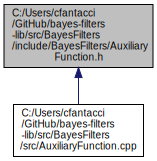
\includegraphics[width=229pt]{AuxiliaryFunction_8h__dep__incl}
\end{center}
\end{figure}

\hypertarget{DrawParticles_8h}{}\section{C\+:/\+Users/cfantacci/\+Git\+Hub/bayes-\/filters-\/lib/src/\+Bayes\+Filters/include/\+Bayes\+Filters/\+Draw\+Particles.h File Reference}
\label{DrawParticles_8h}\index{C\+:/\+Users/cfantacci/\+Git\+Hub/bayes-\/filters-\/lib/src/\+Bayes\+Filters/include/\+Bayes\+Filters/\+Draw\+Particles.\+h@{C\+:/\+Users/cfantacci/\+Git\+Hub/bayes-\/filters-\/lib/src/\+Bayes\+Filters/include/\+Bayes\+Filters/\+Draw\+Particles.\+h}}
{\ttfamily \#include \char`\"{}P\+F\+Prediction.\+h\char`\"{}}\newline
{\ttfamily \#include $<$random$>$}\newline
{\ttfamily \#include $<$memory$>$}\newline
Include dependency graph for Draw\+Particles.\+h\+:
\nopagebreak
\begin{figure}[H]
\begin{center}
\leavevmode
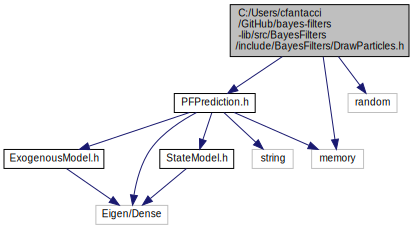
\includegraphics[width=350pt]{DrawParticles_8h__incl}
\end{center}
\end{figure}
This graph shows which files directly or indirectly include this file\+:
\nopagebreak
\begin{figure}[H]
\begin{center}
\leavevmode
\includegraphics[width=259pt]{DrawParticles_8h__dep__incl}
\end{center}
\end{figure}
\subsection*{Classes}
\begin{DoxyCompactItemize}
\item 
class \mbox{\hyperlink{classbfl_1_1DrawParticles}{bfl\+::\+Draw\+Particles}}
\end{DoxyCompactItemize}
\subsection*{Namespaces}
\begin{DoxyCompactItemize}
\item 
 \mbox{\hyperlink{namespacebfl}{bfl}}
\end{DoxyCompactItemize}

\hypertarget{EstimatesExtraction_8h}{}\section{C\+:/\+Users/cfantacci/\+Git\+Hub/bayes-\/filters-\/lib/src/\+Bayes\+Filters/include/\+Bayes\+Filters/\+Estimates\+Extraction.h File Reference}
\label{EstimatesExtraction_8h}\index{C\+:/\+Users/cfantacci/\+Git\+Hub/bayes-\/filters-\/lib/src/\+Bayes\+Filters/include/\+Bayes\+Filters/\+Estimates\+Extraction.\+h@{C\+:/\+Users/cfantacci/\+Git\+Hub/bayes-\/filters-\/lib/src/\+Bayes\+Filters/include/\+Bayes\+Filters/\+Estimates\+Extraction.\+h}}
{\ttfamily \#include $<$string$>$}\newline
{\ttfamily \#include $<$vector$>$}\newline
{\ttfamily \#include $<$Eigen/\+Core$>$}\newline
{\ttfamily \#include $<$Bayes\+Filters/\+History\+Buffer.\+h$>$}\newline
Include dependency graph for Estimates\+Extraction.\+h\+:
\nopagebreak
\begin{figure}[H]
\begin{center}
\leavevmode
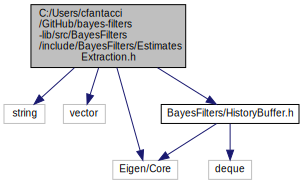
\includegraphics[width=350pt]{EstimatesExtraction_8h__incl}
\end{center}
\end{figure}
This graph shows which files directly or indirectly include this file\+:
\nopagebreak
\begin{figure}[H]
\begin{center}
\leavevmode
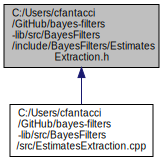
\includegraphics[width=235pt]{EstimatesExtraction_8h__dep__incl}
\end{center}
\end{figure}
\subsection*{Classes}
\begin{DoxyCompactItemize}
\item 
class \mbox{\hyperlink{classbfl_1_1EstimatesExtraction}{bfl\+::\+Estimates\+Extraction}}
\end{DoxyCompactItemize}
\subsection*{Namespaces}
\begin{DoxyCompactItemize}
\item 
 \mbox{\hyperlink{namespacebfl}{bfl}}
\end{DoxyCompactItemize}

\hypertarget{ExogenousModel_8h}{}\section{C\+:/\+Users/cfantacci/\+Git\+Hub/bayes-\/filters-\/lib/src/\+Bayes\+Filters/include/\+Bayes\+Filters/\+Exogenous\+Model.h File Reference}
\label{ExogenousModel_8h}\index{C\+:/\+Users/cfantacci/\+Git\+Hub/bayes-\/filters-\/lib/src/\+Bayes\+Filters/include/\+Bayes\+Filters/\+Exogenous\+Model.\+h@{C\+:/\+Users/cfantacci/\+Git\+Hub/bayes-\/filters-\/lib/src/\+Bayes\+Filters/include/\+Bayes\+Filters/\+Exogenous\+Model.\+h}}
{\ttfamily \#include $<$Eigen/\+Dense$>$}\newline
Include dependency graph for Exogenous\+Model.\+h\+:
\nopagebreak
\begin{figure}[H]
\begin{center}
\leavevmode
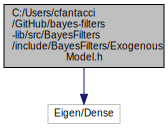
\includegraphics[width=240pt]{ExogenousModel_8h__incl}
\end{center}
\end{figure}
This graph shows which files directly or indirectly include this file\+:
\nopagebreak
\begin{figure}[H]
\begin{center}
\leavevmode
\includegraphics[width=350pt]{ExogenousModel_8h__dep__incl}
\end{center}
\end{figure}
\subsection*{Classes}
\begin{DoxyCompactItemize}
\item 
class \mbox{\hyperlink{classbfl_1_1ExogenousModel}{bfl\+::\+Exogenous\+Model}}
\end{DoxyCompactItemize}
\subsection*{Namespaces}
\begin{DoxyCompactItemize}
\item 
 \mbox{\hyperlink{namespacebfl}{bfl}}
\end{DoxyCompactItemize}

\hypertarget{FilteringAlgorithm_8h}{}\section{C\+:/\+Users/cfantacci/\+Git\+Hub/bayes-\/filters-\/lib/src/\+Bayes\+Filters/include/\+Bayes\+Filters/\+Filtering\+Algorithm.h File Reference}
\label{FilteringAlgorithm_8h}\index{C\+:/\+Users/cfantacci/\+Git\+Hub/bayes-\/filters-\/lib/src/\+Bayes\+Filters/include/\+Bayes\+Filters/\+Filtering\+Algorithm.\+h@{C\+:/\+Users/cfantacci/\+Git\+Hub/bayes-\/filters-\/lib/src/\+Bayes\+Filters/include/\+Bayes\+Filters/\+Filtering\+Algorithm.\+h}}
{\ttfamily \#include $<$condition\+\_\+variable$>$}\newline
{\ttfamily \#include $<$mutex$>$}\newline
{\ttfamily \#include $<$string$>$}\newline
{\ttfamily \#include $<$thread$>$}\newline
{\ttfamily \#include $<$unordered\+\_\+map$>$}\newline
Include dependency graph for Filtering\+Algorithm.\+h\+:
\nopagebreak
\begin{figure}[H]
\begin{center}
\leavevmode
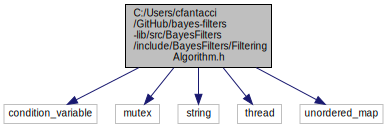
\includegraphics[width=350pt]{FilteringAlgorithm_8h__incl}
\end{center}
\end{figure}
This graph shows which files directly or indirectly include this file\+:
\nopagebreak
\begin{figure}[H]
\begin{center}
\leavevmode
\includegraphics[width=350pt]{FilteringAlgorithm_8h__dep__incl}
\end{center}
\end{figure}
\subsection*{Classes}
\begin{DoxyCompactItemize}
\item 
class \mbox{\hyperlink{classbfl_1_1FilteringAlgorithm}{bfl\+::\+Filtering\+Algorithm}}
\end{DoxyCompactItemize}
\subsection*{Namespaces}
\begin{DoxyCompactItemize}
\item 
 \mbox{\hyperlink{namespacebfl}{bfl}}
\end{DoxyCompactItemize}
\subsection*{Typedefs}
\begin{DoxyCompactItemize}
\item 
typedef std\+::unordered\+\_\+map$<$ std\+::string, double $>$ \mbox{\hyperlink{namespacebfl_aeab050cf5b080512a10c1fec72921f0c}{bfl\+::\+Filtering\+ParamtersD}}
\item 
typedef std\+::unordered\+\_\+map$<$ std\+::string, std\+::string $>$ \mbox{\hyperlink{namespacebfl_aaa1677d9f16c84aac08a5a0bf36a0fa6}{bfl\+::\+Filtering\+ParamtersS}}
\end{DoxyCompactItemize}

\hypertarget{FilteringContext_8h}{}\section{C\+:/\+Users/cfantacci/\+Git\+Hub/bayes-\/filters-\/lib/src/\+Bayes\+Filters/include/\+Bayes\+Filters/\+Filtering\+Context.h File Reference}
\label{FilteringContext_8h}\index{C\+:/\+Users/cfantacci/\+Git\+Hub/bayes-\/filters-\/lib/src/\+Bayes\+Filters/include/\+Bayes\+Filters/\+Filtering\+Context.\+h@{C\+:/\+Users/cfantacci/\+Git\+Hub/bayes-\/filters-\/lib/src/\+Bayes\+Filters/include/\+Bayes\+Filters/\+Filtering\+Context.\+h}}
{\ttfamily \#include $<$memory$>$}\newline
{\ttfamily \#include \char`\"{}Filtering\+Algorithm.\+h\char`\"{}}\newline
Include dependency graph for Filtering\+Context.\+h\+:
\nopagebreak
\begin{figure}[H]
\begin{center}
\leavevmode
\includegraphics[width=350pt]{FilteringContext_8h__incl}
\end{center}
\end{figure}
This graph shows which files directly or indirectly include this file\+:
\nopagebreak
\begin{figure}[H]
\begin{center}
\leavevmode
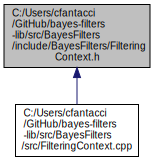
\includegraphics[width=226pt]{FilteringContext_8h__dep__incl}
\end{center}
\end{figure}
\subsection*{Classes}
\begin{DoxyCompactItemize}
\item 
class \mbox{\hyperlink{classbfl_1_1FilteringContext}{bfl\+::\+Filtering\+Context}}
\end{DoxyCompactItemize}
\subsection*{Namespaces}
\begin{DoxyCompactItemize}
\item 
 \mbox{\hyperlink{namespacebfl}{bfl}}
\end{DoxyCompactItemize}

\hypertarget{HistoryBuffer_8h}{}\section{C\+:/\+Users/cfantacci/\+Git\+Hub/bayes-\/filters-\/lib/src/\+Bayes\+Filters/include/\+Bayes\+Filters/\+History\+Buffer.h File Reference}
\label{HistoryBuffer_8h}\index{C\+:/\+Users/cfantacci/\+Git\+Hub/bayes-\/filters-\/lib/src/\+Bayes\+Filters/include/\+Bayes\+Filters/\+History\+Buffer.\+h@{C\+:/\+Users/cfantacci/\+Git\+Hub/bayes-\/filters-\/lib/src/\+Bayes\+Filters/include/\+Bayes\+Filters/\+History\+Buffer.\+h}}
{\ttfamily \#include $<$deque$>$}\newline
{\ttfamily \#include $<$Eigen/\+Core$>$}\newline
Include dependency graph for History\+Buffer.\+h\+:
\nopagebreak
\begin{figure}[H]
\begin{center}
\leavevmode
\includegraphics[width=255pt]{HistoryBuffer_8h__incl}
\end{center}
\end{figure}
This graph shows which files directly or indirectly include this file\+:
\nopagebreak
\begin{figure}[H]
\begin{center}
\leavevmode
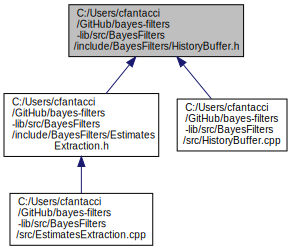
\includegraphics[width=350pt]{HistoryBuffer_8h__dep__incl}
\end{center}
\end{figure}
\subsection*{Classes}
\begin{DoxyCompactItemize}
\item 
class \mbox{\hyperlink{classbfl_1_1HistoryBuffer}{bfl\+::\+History\+Buffer}}
\end{DoxyCompactItemize}
\subsection*{Namespaces}
\begin{DoxyCompactItemize}
\item 
 \mbox{\hyperlink{namespacebfl}{bfl}}
\end{DoxyCompactItemize}

\hypertarget{Initialization_8h}{}\section{C\+:/\+Users/cfantacci/\+Git\+Hub/bayes-\/filters-\/lib/src/\+Bayes\+Filters/include/\+Bayes\+Filters/\+Initialization.h File Reference}
\label{Initialization_8h}\index{C\+:/\+Users/cfantacci/\+Git\+Hub/bayes-\/filters-\/lib/src/\+Bayes\+Filters/include/\+Bayes\+Filters/\+Initialization.\+h@{C\+:/\+Users/cfantacci/\+Git\+Hub/bayes-\/filters-\/lib/src/\+Bayes\+Filters/include/\+Bayes\+Filters/\+Initialization.\+h}}
{\ttfamily \#include $<$Eigen/\+Dense$>$}\newline
Include dependency graph for Initialization.\+h\+:
\nopagebreak
\begin{figure}[H]
\begin{center}
\leavevmode
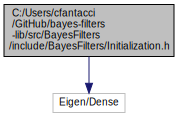
\includegraphics[width=250pt]{Initialization_8h__incl}
\end{center}
\end{figure}
This graph shows which files directly or indirectly include this file\+:
\nopagebreak
\begin{figure}[H]
\begin{center}
\leavevmode
\includegraphics[width=350pt]{Initialization_8h__dep__incl}
\end{center}
\end{figure}
\subsection*{Classes}
\begin{DoxyCompactItemize}
\item 
class \mbox{\hyperlink{classbfl_1_1Initialization}{bfl\+::\+Initialization}}
\end{DoxyCompactItemize}
\subsection*{Namespaces}
\begin{DoxyCompactItemize}
\item 
 \mbox{\hyperlink{namespacebfl}{bfl}}
\end{DoxyCompactItemize}

\hypertarget{KalmanFilter_8h}{}\section{C\+:/\+Users/cfantacci/\+Git\+Hub/bayes-\/filters-\/lib/src/\+Bayes\+Filters/include/\+Bayes\+Filters/\+Kalman\+Filter.h File Reference}
\label{KalmanFilter_8h}\index{C\+:/\+Users/cfantacci/\+Git\+Hub/bayes-\/filters-\/lib/src/\+Bayes\+Filters/include/\+Bayes\+Filters/\+Kalman\+Filter.\+h@{C\+:/\+Users/cfantacci/\+Git\+Hub/bayes-\/filters-\/lib/src/\+Bayes\+Filters/include/\+Bayes\+Filters/\+Kalman\+Filter.\+h}}
{\ttfamily \#include \char`\"{}Filtering\+Algorithm.\+h\char`\"{}}\newline
Include dependency graph for Kalman\+Filter.\+h\+:
\nopagebreak
\begin{figure}[H]
\begin{center}
\leavevmode
\includegraphics[width=350pt]{KalmanFilter_8h__incl}
\end{center}
\end{figure}
This graph shows which files directly or indirectly include this file\+:
\nopagebreak
\begin{figure}[H]
\begin{center}
\leavevmode
\includegraphics[width=254pt]{KalmanFilter_8h__dep__incl}
\end{center}
\end{figure}
\subsection*{Classes}
\begin{DoxyCompactItemize}
\item 
class \mbox{\hyperlink{classbfl_1_1KalmanFilter}{bfl\+::\+Kalman\+Filter}}
\end{DoxyCompactItemize}
\subsection*{Namespaces}
\begin{DoxyCompactItemize}
\item 
 \mbox{\hyperlink{namespacebfl}{bfl}}
\end{DoxyCompactItemize}

\hypertarget{LinearSensor_8h}{}\section{C\+:/\+Users/cfantacci/\+Git\+Hub/bayes-\/filters-\/lib/src/\+Bayes\+Filters/include/\+Bayes\+Filters/\+Linear\+Sensor.h File Reference}
\label{LinearSensor_8h}\index{C\+:/\+Users/cfantacci/\+Git\+Hub/bayes-\/filters-\/lib/src/\+Bayes\+Filters/include/\+Bayes\+Filters/\+Linear\+Sensor.\+h@{C\+:/\+Users/cfantacci/\+Git\+Hub/bayes-\/filters-\/lib/src/\+Bayes\+Filters/include/\+Bayes\+Filters/\+Linear\+Sensor.\+h}}
{\ttfamily \#include $<$functional$>$}\newline
{\ttfamily \#include $<$random$>$}\newline
{\ttfamily \#include \char`\"{}Observation\+Model.\+h\char`\"{}}\newline
Include dependency graph for Linear\+Sensor.\+h\+:
\nopagebreak
\begin{figure}[H]
\begin{center}
\leavevmode
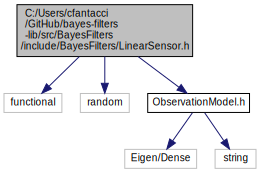
\includegraphics[width=333pt]{LinearSensor_8h__incl}
\end{center}
\end{figure}
This graph shows which files directly or indirectly include this file\+:
\nopagebreak
\begin{figure}[H]
\begin{center}
\leavevmode
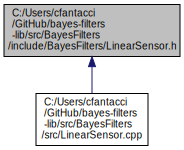
\includegraphics[width=256pt]{LinearSensor_8h__dep__incl}
\end{center}
\end{figure}
\subsection*{Classes}
\begin{DoxyCompactItemize}
\item 
class \mbox{\hyperlink{classbfl_1_1LinearSensor}{bfl\+::\+Linear\+Sensor}}
\end{DoxyCompactItemize}
\subsection*{Namespaces}
\begin{DoxyCompactItemize}
\item 
 \mbox{\hyperlink{namespacebfl}{bfl}}
\end{DoxyCompactItemize}

\hypertarget{ObservationModel_8h}{}\section{C\+:/\+Users/cfantacci/\+Git\+Hub/bayes-\/filters-\/lib/src/\+Bayes\+Filters/include/\+Bayes\+Filters/\+Observation\+Model.h File Reference}
\label{ObservationModel_8h}\index{C\+:/\+Users/cfantacci/\+Git\+Hub/bayes-\/filters-\/lib/src/\+Bayes\+Filters/include/\+Bayes\+Filters/\+Observation\+Model.\+h@{C\+:/\+Users/cfantacci/\+Git\+Hub/bayes-\/filters-\/lib/src/\+Bayes\+Filters/include/\+Bayes\+Filters/\+Observation\+Model.\+h}}
{\ttfamily \#include $<$Eigen/\+Dense$>$}\newline
{\ttfamily \#include $<$string$>$}\newline
Include dependency graph for Observation\+Model.\+h\+:
\nopagebreak
\begin{figure}[H]
\begin{center}
\leavevmode
\includegraphics[width=242pt]{ObservationModel_8h__incl}
\end{center}
\end{figure}
This graph shows which files directly or indirectly include this file\+:
\nopagebreak
\begin{figure}[H]
\begin{center}
\leavevmode
\includegraphics[width=350pt]{ObservationModel_8h__dep__incl}
\end{center}
\end{figure}
\subsection*{Classes}
\begin{DoxyCompactItemize}
\item 
class \mbox{\hyperlink{classbfl_1_1ObservationModel}{bfl\+::\+Observation\+Model}}
\end{DoxyCompactItemize}
\subsection*{Namespaces}
\begin{DoxyCompactItemize}
\item 
 \mbox{\hyperlink{namespacebfl}{bfl}}
\end{DoxyCompactItemize}

\hypertarget{ObservationModelDecorator_8h}{}\section{C\+:/\+Users/cfantacci/\+Git\+Hub/bayes-\/filters-\/lib/src/\+Bayes\+Filters/include/\+Bayes\+Filters/\+Observation\+Model\+Decorator.h File Reference}
\label{ObservationModelDecorator_8h}\index{C\+:/\+Users/cfantacci/\+Git\+Hub/bayes-\/filters-\/lib/src/\+Bayes\+Filters/include/\+Bayes\+Filters/\+Observation\+Model\+Decorator.\+h@{C\+:/\+Users/cfantacci/\+Git\+Hub/bayes-\/filters-\/lib/src/\+Bayes\+Filters/include/\+Bayes\+Filters/\+Observation\+Model\+Decorator.\+h}}
{\ttfamily \#include \char`\"{}Observation\+Model.\+h\char`\"{}}\newline
{\ttfamily \#include $<$memory$>$}\newline
Include dependency graph for Observation\+Model\+Decorator.\+h\+:
\nopagebreak
\begin{figure}[H]
\begin{center}
\leavevmode
\includegraphics[width=281pt]{ObservationModelDecorator_8h__incl}
\end{center}
\end{figure}
This graph shows which files directly or indirectly include this file\+:
\nopagebreak
\begin{figure}[H]
\begin{center}
\leavevmode
\includegraphics[width=254pt]{ObservationModelDecorator_8h__dep__incl}
\end{center}
\end{figure}
\subsection*{Classes}
\begin{DoxyCompactItemize}
\item 
class \mbox{\hyperlink{classbfl_1_1ObservationModelDecorator}{bfl\+::\+Observation\+Model\+Decorator}}
\end{DoxyCompactItemize}
\subsection*{Namespaces}
\begin{DoxyCompactItemize}
\item 
 \mbox{\hyperlink{namespacebfl}{bfl}}
\end{DoxyCompactItemize}

\hypertarget{ParticleFilter_8h}{}\section{C\+:/\+Users/cfantacci/\+Git\+Hub/bayes-\/filters-\/lib/src/\+Bayes\+Filters/include/\+Bayes\+Filters/\+Particle\+Filter.h File Reference}
\label{ParticleFilter_8h}\index{C\+:/\+Users/cfantacci/\+Git\+Hub/bayes-\/filters-\/lib/src/\+Bayes\+Filters/include/\+Bayes\+Filters/\+Particle\+Filter.\+h@{C\+:/\+Users/cfantacci/\+Git\+Hub/bayes-\/filters-\/lib/src/\+Bayes\+Filters/include/\+Bayes\+Filters/\+Particle\+Filter.\+h}}
{\ttfamily \#include \char`\"{}Filtering\+Algorithm.\+h\char`\"{}}\newline
{\ttfamily \#include \char`\"{}Initialization.\+h\char`\"{}}\newline
{\ttfamily \#include \char`\"{}P\+F\+Correction.\+h\char`\"{}}\newline
{\ttfamily \#include \char`\"{}P\+F\+Prediction.\+h\char`\"{}}\newline
{\ttfamily \#include \char`\"{}Resampling.\+h\char`\"{}}\newline
{\ttfamily \#include $<$memory$>$}\newline
Include dependency graph for Particle\+Filter.\+h\+:
\nopagebreak
\begin{figure}[H]
\begin{center}
\leavevmode
\includegraphics[width=350pt]{ParticleFilter_8h__incl}
\end{center}
\end{figure}
This graph shows which files directly or indirectly include this file\+:
\nopagebreak
\begin{figure}[H]
\begin{center}
\leavevmode
\includegraphics[width=344pt]{ParticleFilter_8h__dep__incl}
\end{center}
\end{figure}
\subsection*{Classes}
\begin{DoxyCompactItemize}
\item 
class \mbox{\hyperlink{classbfl_1_1ParticleFilter}{bfl\+::\+Particle\+Filter}}
\end{DoxyCompactItemize}
\subsection*{Namespaces}
\begin{DoxyCompactItemize}
\item 
 \mbox{\hyperlink{namespacebfl}{bfl}}
\end{DoxyCompactItemize}

\hypertarget{PFCorrection_8h}{}\section{C\+:/\+Users/cfantacci/\+Git\+Hub/bayes-\/filters-\/lib/src/\+Bayes\+Filters/include/\+Bayes\+Filters/\+P\+F\+Correction.h File Reference}
\label{PFCorrection_8h}\index{C\+:/\+Users/cfantacci/\+Git\+Hub/bayes-\/filters-\/lib/src/\+Bayes\+Filters/include/\+Bayes\+Filters/\+P\+F\+Correction.\+h@{C\+:/\+Users/cfantacci/\+Git\+Hub/bayes-\/filters-\/lib/src/\+Bayes\+Filters/include/\+Bayes\+Filters/\+P\+F\+Correction.\+h}}
{\ttfamily \#include \char`\"{}Observation\+Model.\+h\char`\"{}}\newline
{\ttfamily \#include $<$memory$>$}\newline
{\ttfamily \#include $<$Eigen/\+Dense$>$}\newline
Include dependency graph for P\+F\+Correction.\+h\+:
\nopagebreak
\begin{figure}[H]
\begin{center}
\leavevmode
\includegraphics[width=314pt]{PFCorrection_8h__incl}
\end{center}
\end{figure}
This graph shows which files directly or indirectly include this file\+:
\nopagebreak
\begin{figure}[H]
\begin{center}
\leavevmode
\includegraphics[width=350pt]{PFCorrection_8h__dep__incl}
\end{center}
\end{figure}
\subsection*{Classes}
\begin{DoxyCompactItemize}
\item 
class \mbox{\hyperlink{classbfl_1_1PFCorrection}{bfl\+::\+P\+F\+Correction}}
\end{DoxyCompactItemize}
\subsection*{Namespaces}
\begin{DoxyCompactItemize}
\item 
 \mbox{\hyperlink{namespacebfl}{bfl}}
\end{DoxyCompactItemize}

\hypertarget{PFCorrectionDecorator_8h}{}\section{C\+:/\+Users/cfantacci/\+Git\+Hub/bayes-\/filters-\/lib/src/\+Bayes\+Filters/include/\+Bayes\+Filters/\+P\+F\+Correction\+Decorator.h File Reference}
\label{PFCorrectionDecorator_8h}\index{C\+:/\+Users/cfantacci/\+Git\+Hub/bayes-\/filters-\/lib/src/\+Bayes\+Filters/include/\+Bayes\+Filters/\+P\+F\+Correction\+Decorator.\+h@{C\+:/\+Users/cfantacci/\+Git\+Hub/bayes-\/filters-\/lib/src/\+Bayes\+Filters/include/\+Bayes\+Filters/\+P\+F\+Correction\+Decorator.\+h}}
{\ttfamily \#include \char`\"{}P\+F\+Correction.\+h\char`\"{}}\newline
{\ttfamily \#include $<$memory$>$}\newline
Include dependency graph for P\+F\+Correction\+Decorator.\+h\+:
\nopagebreak
\begin{figure}[H]
\begin{center}
\leavevmode
\includegraphics[width=324pt]{PFCorrectionDecorator_8h__incl}
\end{center}
\end{figure}
This graph shows which files directly or indirectly include this file\+:
\nopagebreak
\begin{figure}[H]
\begin{center}
\leavevmode
\includegraphics[width=248pt]{PFCorrectionDecorator_8h__dep__incl}
\end{center}
\end{figure}
\subsection*{Classes}
\begin{DoxyCompactItemize}
\item 
class \mbox{\hyperlink{classbfl_1_1PFCorrectionDecorator}{bfl\+::\+P\+F\+Correction\+Decorator}}
\end{DoxyCompactItemize}
\subsection*{Namespaces}
\begin{DoxyCompactItemize}
\item 
 \mbox{\hyperlink{namespacebfl}{bfl}}
\end{DoxyCompactItemize}

\hypertarget{PFPrediction_8h}{}\section{C\+:/\+Users/cfantacci/\+Git\+Hub/bayes-\/filters-\/lib/src/\+Bayes\+Filters/include/\+Bayes\+Filters/\+P\+F\+Prediction.h File Reference}
\label{PFPrediction_8h}\index{C\+:/\+Users/cfantacci/\+Git\+Hub/bayes-\/filters-\/lib/src/\+Bayes\+Filters/include/\+Bayes\+Filters/\+P\+F\+Prediction.\+h@{C\+:/\+Users/cfantacci/\+Git\+Hub/bayes-\/filters-\/lib/src/\+Bayes\+Filters/include/\+Bayes\+Filters/\+P\+F\+Prediction.\+h}}
{\ttfamily \#include \char`\"{}Exogenous\+Model.\+h\char`\"{}}\newline
{\ttfamily \#include \char`\"{}State\+Model.\+h\char`\"{}}\newline
{\ttfamily \#include $<$Eigen/\+Dense$>$}\newline
{\ttfamily \#include $<$memory$>$}\newline
{\ttfamily \#include $<$string$>$}\newline
Include dependency graph for P\+F\+Prediction.\+h\+:
\nopagebreak
\begin{figure}[H]
\begin{center}
\leavevmode
\includegraphics[width=350pt]{PFPrediction_8h__incl}
\end{center}
\end{figure}
This graph shows which files directly or indirectly include this file\+:
\nopagebreak
\begin{figure}[H]
\begin{center}
\leavevmode
\includegraphics[width=350pt]{PFPrediction_8h__dep__incl}
\end{center}
\end{figure}
\subsection*{Classes}
\begin{DoxyCompactItemize}
\item 
class \mbox{\hyperlink{classbfl_1_1PFPrediction}{bfl\+::\+P\+F\+Prediction}}
\end{DoxyCompactItemize}
\subsection*{Namespaces}
\begin{DoxyCompactItemize}
\item 
 \mbox{\hyperlink{namespacebfl}{bfl}}
\end{DoxyCompactItemize}

\hypertarget{PFPredictionDecorator_8h}{}\section{C\+:/\+Users/cfantacci/\+Git\+Hub/bayes-\/filters-\/lib/src/\+Bayes\+Filters/include/\+Bayes\+Filters/\+P\+F\+Prediction\+Decorator.h File Reference}
\label{PFPredictionDecorator_8h}\index{C\+:/\+Users/cfantacci/\+Git\+Hub/bayes-\/filters-\/lib/src/\+Bayes\+Filters/include/\+Bayes\+Filters/\+P\+F\+Prediction\+Decorator.\+h@{C\+:/\+Users/cfantacci/\+Git\+Hub/bayes-\/filters-\/lib/src/\+Bayes\+Filters/include/\+Bayes\+Filters/\+P\+F\+Prediction\+Decorator.\+h}}
{\ttfamily \#include \char`\"{}P\+F\+Prediction.\+h\char`\"{}}\newline
{\ttfamily \#include $<$memory$>$}\newline
Include dependency graph for P\+F\+Prediction\+Decorator.\+h\+:
\nopagebreak
\begin{figure}[H]
\begin{center}
\leavevmode
\includegraphics[width=350pt]{PFPredictionDecorator_8h__incl}
\end{center}
\end{figure}
This graph shows which files directly or indirectly include this file\+:
\nopagebreak
\begin{figure}[H]
\begin{center}
\leavevmode
\includegraphics[width=247pt]{PFPredictionDecorator_8h__dep__incl}
\end{center}
\end{figure}
\subsection*{Classes}
\begin{DoxyCompactItemize}
\item 
class \mbox{\hyperlink{classbfl_1_1PFPredictionDecorator}{bfl\+::\+P\+F\+Prediction\+Decorator}}
\end{DoxyCompactItemize}
\subsection*{Namespaces}
\begin{DoxyCompactItemize}
\item 
 \mbox{\hyperlink{namespacebfl}{bfl}}
\end{DoxyCompactItemize}

\hypertarget{PFVisualCorrection_8h}{}\section{C\+:/\+Users/cfantacci/\+Git\+Hub/bayes-\/filters-\/lib/src/\+Bayes\+Filters/include/\+Bayes\+Filters/\+P\+F\+Visual\+Correction.h File Reference}
\label{PFVisualCorrection_8h}\index{C\+:/\+Users/cfantacci/\+Git\+Hub/bayes-\/filters-\/lib/src/\+Bayes\+Filters/include/\+Bayes\+Filters/\+P\+F\+Visual\+Correction.\+h@{C\+:/\+Users/cfantacci/\+Git\+Hub/bayes-\/filters-\/lib/src/\+Bayes\+Filters/include/\+Bayes\+Filters/\+P\+F\+Visual\+Correction.\+h}}
{\ttfamily \#include \char`\"{}Visual\+Observation\+Model.\+h\char`\"{}}\newline
{\ttfamily \#include $<$memory$>$}\newline
{\ttfamily \#include $<$Eigen/\+Dense$>$}\newline
{\ttfamily \#include $<$opencv2/core/core.\+hpp$>$}\newline
Include dependency graph for P\+F\+Visual\+Correction.\+h\+:
\nopagebreak
\begin{figure}[H]
\begin{center}
\leavevmode
\includegraphics[width=350pt]{PFVisualCorrection_8h__incl}
\end{center}
\end{figure}
This graph shows which files directly or indirectly include this file\+:
\nopagebreak
\begin{figure}[H]
\begin{center}
\leavevmode
\includegraphics[width=350pt]{PFVisualCorrection_8h__dep__incl}
\end{center}
\end{figure}
\subsection*{Classes}
\begin{DoxyCompactItemize}
\item 
class \mbox{\hyperlink{classbfl_1_1PFVisualCorrection}{bfl\+::\+P\+F\+Visual\+Correction}}
\end{DoxyCompactItemize}
\subsection*{Namespaces}
\begin{DoxyCompactItemize}
\item 
 \mbox{\hyperlink{namespacebfl}{bfl}}
\end{DoxyCompactItemize}

\hypertarget{PFVisualCorrectionDecorator_8h}{}\section{C\+:/\+Users/cfantacci/\+Git\+Hub/bayes-\/filters-\/lib/src/\+Bayes\+Filters/include/\+Bayes\+Filters/\+P\+F\+Visual\+Correction\+Decorator.h File Reference}
\label{PFVisualCorrectionDecorator_8h}\index{C\+:/\+Users/cfantacci/\+Git\+Hub/bayes-\/filters-\/lib/src/\+Bayes\+Filters/include/\+Bayes\+Filters/\+P\+F\+Visual\+Correction\+Decorator.\+h@{C\+:/\+Users/cfantacci/\+Git\+Hub/bayes-\/filters-\/lib/src/\+Bayes\+Filters/include/\+Bayes\+Filters/\+P\+F\+Visual\+Correction\+Decorator.\+h}}
{\ttfamily \#include \char`\"{}P\+F\+Visual\+Correction.\+h\char`\"{}}\newline
{\ttfamily \#include $<$memory$>$}\newline
Include dependency graph for P\+F\+Visual\+Correction\+Decorator.\+h\+:
\nopagebreak
\begin{figure}[H]
\begin{center}
\leavevmode
\includegraphics[width=350pt]{PFVisualCorrectionDecorator_8h__incl}
\end{center}
\end{figure}
This graph shows which files directly or indirectly include this file\+:
\nopagebreak
\begin{figure}[H]
\begin{center}
\leavevmode
\includegraphics[width=261pt]{PFVisualCorrectionDecorator_8h__dep__incl}
\end{center}
\end{figure}
\subsection*{Classes}
\begin{DoxyCompactItemize}
\item 
class \mbox{\hyperlink{classbfl_1_1PFVisualCorrectionDecorator}{bfl\+::\+P\+F\+Visual\+Correction\+Decorator}}
\end{DoxyCompactItemize}
\subsection*{Namespaces}
\begin{DoxyCompactItemize}
\item 
 \mbox{\hyperlink{namespacebfl}{bfl}}
\end{DoxyCompactItemize}

\hypertarget{Resampling_8h}{}\section{C\+:/\+Users/cfantacci/\+Git\+Hub/bayes-\/filters-\/lib/src/\+Bayes\+Filters/include/\+Bayes\+Filters/\+Resampling.h File Reference}
\label{Resampling_8h}\index{C\+:/\+Users/cfantacci/\+Git\+Hub/bayes-\/filters-\/lib/src/\+Bayes\+Filters/include/\+Bayes\+Filters/\+Resampling.\+h@{C\+:/\+Users/cfantacci/\+Git\+Hub/bayes-\/filters-\/lib/src/\+Bayes\+Filters/include/\+Bayes\+Filters/\+Resampling.\+h}}
{\ttfamily \#include $<$random$>$}\newline
{\ttfamily \#include $<$Eigen/\+Dense$>$}\newline
Include dependency graph for Resampling.\+h\+:
\nopagebreak
\begin{figure}[H]
\begin{center}
\leavevmode
\includegraphics[width=250pt]{Resampling_8h__incl}
\end{center}
\end{figure}
This graph shows which files directly or indirectly include this file\+:
\nopagebreak
\begin{figure}[H]
\begin{center}
\leavevmode
\includegraphics[width=350pt]{Resampling_8h__dep__incl}
\end{center}
\end{figure}
\subsection*{Classes}
\begin{DoxyCompactItemize}
\item 
class \mbox{\hyperlink{classbfl_1_1Resampling}{bfl\+::\+Resampling}}
\end{DoxyCompactItemize}
\subsection*{Namespaces}
\begin{DoxyCompactItemize}
\item 
 \mbox{\hyperlink{namespacebfl}{bfl}}
\end{DoxyCompactItemize}

\hypertarget{ResamplingWithPrior_8h}{}\section{C\+:/\+Users/cfantacci/\+Git\+Hub/bayes-\/filters-\/lib/src/\+Bayes\+Filters/include/\+Bayes\+Filters/\+Resampling\+With\+Prior.h File Reference}
\label{ResamplingWithPrior_8h}\index{C\+:/\+Users/cfantacci/\+Git\+Hub/bayes-\/filters-\/lib/src/\+Bayes\+Filters/include/\+Bayes\+Filters/\+Resampling\+With\+Prior.\+h@{C\+:/\+Users/cfantacci/\+Git\+Hub/bayes-\/filters-\/lib/src/\+Bayes\+Filters/include/\+Bayes\+Filters/\+Resampling\+With\+Prior.\+h}}
{\ttfamily \#include $<$memory$>$}\newline
{\ttfamily \#include $<$vector$>$}\newline
{\ttfamily \#include $<$Bayes\+Filters/\+Initialization.\+h$>$}\newline
{\ttfamily \#include $<$Bayes\+Filters/\+Resampling.\+h$>$}\newline
{\ttfamily \#include $<$Eigen/\+Dense$>$}\newline
Include dependency graph for Resampling\+With\+Prior.\+h\+:
\nopagebreak
\begin{figure}[H]
\begin{center}
\leavevmode
\includegraphics[width=350pt]{ResamplingWithPrior_8h__incl}
\end{center}
\end{figure}
This graph shows which files directly or indirectly include this file\+:
\nopagebreak
\begin{figure}[H]
\begin{center}
\leavevmode
\includegraphics[width=242pt]{ResamplingWithPrior_8h__dep__incl}
\end{center}
\end{figure}
\subsection*{Classes}
\begin{DoxyCompactItemize}
\item 
class \mbox{\hyperlink{classbfl_1_1ResamplingWithPrior}{bfl\+::\+Resampling\+With\+Prior}}
\end{DoxyCompactItemize}
\subsection*{Namespaces}
\begin{DoxyCompactItemize}
\item 
 \mbox{\hyperlink{namespacebfl}{bfl}}
\end{DoxyCompactItemize}

\hypertarget{SigmaPointTransform_8h}{}\section{C\+:/\+Users/cfantacci/\+Git\+Hub/bayes-\/filters-\/lib/src/\+Bayes\+Filters/include/\+Bayes\+Filters/\+Sigma\+Point\+Transform.h File Reference}
\label{SigmaPointTransform_8h}\index{C\+:/\+Users/cfantacci/\+Git\+Hub/bayes-\/filters-\/lib/src/\+Bayes\+Filters/include/\+Bayes\+Filters/\+Sigma\+Point\+Transform.\+h@{C\+:/\+Users/cfantacci/\+Git\+Hub/bayes-\/filters-\/lib/src/\+Bayes\+Filters/include/\+Bayes\+Filters/\+Sigma\+Point\+Transform.\+h}}

\hypertarget{SIS_8h}{}\section{C\+:/\+Users/cfantacci/\+Git\+Hub/bayes-\/filters-\/lib/src/\+Bayes\+Filters/include/\+Bayes\+Filters/\+S\+IS.h File Reference}
\label{SIS_8h}\index{C\+:/\+Users/cfantacci/\+Git\+Hub/bayes-\/filters-\/lib/src/\+Bayes\+Filters/include/\+Bayes\+Filters/\+S\+I\+S.\+h@{C\+:/\+Users/cfantacci/\+Git\+Hub/bayes-\/filters-\/lib/src/\+Bayes\+Filters/include/\+Bayes\+Filters/\+S\+I\+S.\+h}}
{\ttfamily \#include \char`\"{}Particle\+Filter.\+h\char`\"{}}\newline
{\ttfamily \#include \char`\"{}P\+F\+Correction.\+h\char`\"{}}\newline
{\ttfamily \#include \char`\"{}P\+F\+Prediction.\+h\char`\"{}}\newline
{\ttfamily \#include \char`\"{}Resampling.\+h\char`\"{}}\newline
{\ttfamily \#include $<$memory$>$}\newline
{\ttfamily \#include $<$Eigen/\+Dense$>$}\newline
Include dependency graph for S\+I\+S.\+h\+:
\nopagebreak
\begin{figure}[H]
\begin{center}
\leavevmode
\includegraphics[width=350pt]{SIS_8h__incl}
\end{center}
\end{figure}
This graph shows which files directly or indirectly include this file\+:
\nopagebreak
\begin{figure}[H]
\begin{center}
\leavevmode
\includegraphics[width=215pt]{SIS_8h__dep__incl}
\end{center}
\end{figure}
\subsection*{Classes}
\begin{DoxyCompactItemize}
\item 
class \mbox{\hyperlink{classbfl_1_1SIS}{bfl\+::\+S\+IS}}
\end{DoxyCompactItemize}
\subsection*{Namespaces}
\begin{DoxyCompactItemize}
\item 
 \mbox{\hyperlink{namespacebfl}{bfl}}
\end{DoxyCompactItemize}

\hypertarget{StateModel_8h}{}\section{C\+:/\+Users/cfantacci/\+Git\+Hub/bayes-\/filters-\/lib/src/\+Bayes\+Filters/include/\+Bayes\+Filters/\+State\+Model.h File Reference}
\label{StateModel_8h}\index{C\+:/\+Users/cfantacci/\+Git\+Hub/bayes-\/filters-\/lib/src/\+Bayes\+Filters/include/\+Bayes\+Filters/\+State\+Model.\+h@{C\+:/\+Users/cfantacci/\+Git\+Hub/bayes-\/filters-\/lib/src/\+Bayes\+Filters/include/\+Bayes\+Filters/\+State\+Model.\+h}}
{\ttfamily \#include $<$Eigen/\+Dense$>$}\newline
Include dependency graph for State\+Model.\+h\+:
\nopagebreak
\begin{figure}[H]
\begin{center}
\leavevmode
\includegraphics[width=249pt]{StateModel_8h__incl}
\end{center}
\end{figure}
This graph shows which files directly or indirectly include this file\+:
\nopagebreak
\begin{figure}[H]
\begin{center}
\leavevmode
\includegraphics[width=350pt]{StateModel_8h__dep__incl}
\end{center}
\end{figure}
\subsection*{Classes}
\begin{DoxyCompactItemize}
\item 
class \mbox{\hyperlink{classbfl_1_1StateModel}{bfl\+::\+State\+Model}}
\end{DoxyCompactItemize}
\subsection*{Namespaces}
\begin{DoxyCompactItemize}
\item 
 \mbox{\hyperlink{namespacebfl}{bfl}}
\end{DoxyCompactItemize}

\hypertarget{StateModelDecorator_8h}{}\section{C\+:/\+Users/cfantacci/\+Git\+Hub/bayes-\/filters-\/lib/src/\+Bayes\+Filters/include/\+Bayes\+Filters/\+State\+Model\+Decorator.h File Reference}
\label{StateModelDecorator_8h}\index{C\+:/\+Users/cfantacci/\+Git\+Hub/bayes-\/filters-\/lib/src/\+Bayes\+Filters/include/\+Bayes\+Filters/\+State\+Model\+Decorator.\+h@{C\+:/\+Users/cfantacci/\+Git\+Hub/bayes-\/filters-\/lib/src/\+Bayes\+Filters/include/\+Bayes\+Filters/\+State\+Model\+Decorator.\+h}}
{\ttfamily \#include \char`\"{}State\+Model.\+h\char`\"{}}\newline
{\ttfamily \#include $<$memory$>$}\newline
Include dependency graph for State\+Model\+Decorator.\+h\+:
\nopagebreak
\begin{figure}[H]
\begin{center}
\leavevmode
\includegraphics[width=241pt]{StateModelDecorator_8h__incl}
\end{center}
\end{figure}
This graph shows which files directly or indirectly include this file\+:
\nopagebreak
\begin{figure}[H]
\begin{center}
\leavevmode
\includegraphics[width=241pt]{StateModelDecorator_8h__dep__incl}
\end{center}
\end{figure}
\subsection*{Classes}
\begin{DoxyCompactItemize}
\item 
class \mbox{\hyperlink{classbfl_1_1StateModelDecorator}{bfl\+::\+State\+Model\+Decorator}}
\end{DoxyCompactItemize}
\subsection*{Namespaces}
\begin{DoxyCompactItemize}
\item 
 \mbox{\hyperlink{namespacebfl}{bfl}}
\end{DoxyCompactItemize}

\hypertarget{UnscentedKalmanFilter_8h}{}\section{C\+:/\+Users/cfantacci/\+Git\+Hub/bayes-\/filters-\/lib/src/\+Bayes\+Filters/include/\+Bayes\+Filters/\+Unscented\+Kalman\+Filter.h File Reference}
\label{UnscentedKalmanFilter_8h}\index{C\+:/\+Users/cfantacci/\+Git\+Hub/bayes-\/filters-\/lib/src/\+Bayes\+Filters/include/\+Bayes\+Filters/\+Unscented\+Kalman\+Filter.\+h@{C\+:/\+Users/cfantacci/\+Git\+Hub/bayes-\/filters-\/lib/src/\+Bayes\+Filters/include/\+Bayes\+Filters/\+Unscented\+Kalman\+Filter.\+h}}
{\ttfamily \#include \char`\"{}Filtering\+Algorithm.\+h\char`\"{}}\newline
Include dependency graph for Unscented\+Kalman\+Filter.\+h\+:
\nopagebreak
\begin{figure}[H]
\begin{center}
\leavevmode
\includegraphics[width=350pt]{UnscentedKalmanFilter_8h__incl}
\end{center}
\end{figure}
This graph shows which files directly or indirectly include this file\+:
\nopagebreak
\begin{figure}[H]
\begin{center}
\leavevmode
\includegraphics[width=238pt]{UnscentedKalmanFilter_8h__dep__incl}
\end{center}
\end{figure}
\subsection*{Classes}
\begin{DoxyCompactItemize}
\item 
class \mbox{\hyperlink{classbfl_1_1UnscentedKalmanFilter}{bfl\+::\+Unscented\+Kalman\+Filter}}
\end{DoxyCompactItemize}
\subsection*{Namespaces}
\begin{DoxyCompactItemize}
\item 
 \mbox{\hyperlink{namespacebfl}{bfl}}
\end{DoxyCompactItemize}

\hypertarget{UpdateParticles_8h}{}\section{C\+:/\+Users/cfantacci/\+Git\+Hub/bayes-\/filters-\/lib/src/\+Bayes\+Filters/include/\+Bayes\+Filters/\+Update\+Particles.h File Reference}
\label{UpdateParticles_8h}\index{C\+:/\+Users/cfantacci/\+Git\+Hub/bayes-\/filters-\/lib/src/\+Bayes\+Filters/include/\+Bayes\+Filters/\+Update\+Particles.\+h@{C\+:/\+Users/cfantacci/\+Git\+Hub/bayes-\/filters-\/lib/src/\+Bayes\+Filters/include/\+Bayes\+Filters/\+Update\+Particles.\+h}}
{\ttfamily \#include \char`\"{}P\+F\+Correction.\+h\char`\"{}}\newline
{\ttfamily \#include $<$memory$>$}\newline
{\ttfamily \#include $<$random$>$}\newline
Include dependency graph for Update\+Particles.\+h\+:
\nopagebreak
\begin{figure}[H]
\begin{center}
\leavevmode
\includegraphics[width=350pt]{UpdateParticles_8h__incl}
\end{center}
\end{figure}
This graph shows which files directly or indirectly include this file\+:
\nopagebreak
\begin{figure}[H]
\begin{center}
\leavevmode
\includegraphics[width=268pt]{UpdateParticles_8h__dep__incl}
\end{center}
\end{figure}
\subsection*{Classes}
\begin{DoxyCompactItemize}
\item 
class \mbox{\hyperlink{classbfl_1_1UpdateParticles}{bfl\+::\+Update\+Particles}}
\end{DoxyCompactItemize}
\subsection*{Namespaces}
\begin{DoxyCompactItemize}
\item 
 \mbox{\hyperlink{namespacebfl}{bfl}}
\end{DoxyCompactItemize}

\hypertarget{VisualObservationModel_8h}{}\section{C\+:/\+Users/cfantacci/\+Git\+Hub/bayes-\/filters-\/lib/src/\+Bayes\+Filters/include/\+Bayes\+Filters/\+Visual\+Observation\+Model.h File Reference}
\label{VisualObservationModel_8h}\index{C\+:/\+Users/cfantacci/\+Git\+Hub/bayes-\/filters-\/lib/src/\+Bayes\+Filters/include/\+Bayes\+Filters/\+Visual\+Observation\+Model.\+h@{C\+:/\+Users/cfantacci/\+Git\+Hub/bayes-\/filters-\/lib/src/\+Bayes\+Filters/include/\+Bayes\+Filters/\+Visual\+Observation\+Model.\+h}}
{\ttfamily \#include $<$Eigen/\+Dense$>$}\newline
{\ttfamily \#include $<$opencv2/core/core.\+hpp$>$}\newline
{\ttfamily \#include $<$string$>$}\newline
Include dependency graph for Visual\+Observation\+Model.\+h\+:
\nopagebreak
\begin{figure}[H]
\begin{center}
\leavevmode
\includegraphics[width=344pt]{VisualObservationModel_8h__incl}
\end{center}
\end{figure}
This graph shows which files directly or indirectly include this file\+:
\nopagebreak
\begin{figure}[H]
\begin{center}
\leavevmode
\includegraphics[width=350pt]{VisualObservationModel_8h__dep__incl}
\end{center}
\end{figure}
\subsection*{Classes}
\begin{DoxyCompactItemize}
\item 
class \mbox{\hyperlink{classbfl_1_1VisualObservationModel}{bfl\+::\+Visual\+Observation\+Model}}
\end{DoxyCompactItemize}
\subsection*{Namespaces}
\begin{DoxyCompactItemize}
\item 
 \mbox{\hyperlink{namespacebfl}{bfl}}
\end{DoxyCompactItemize}

\hypertarget{VisualParticleFilter_8h}{}\section{C\+:/\+Users/cfantacci/\+Git\+Hub/bayes-\/filters-\/lib/src/\+Bayes\+Filters/include/\+Bayes\+Filters/\+Visual\+Particle\+Filter.h File Reference}
\label{VisualParticleFilter_8h}\index{C\+:/\+Users/cfantacci/\+Git\+Hub/bayes-\/filters-\/lib/src/\+Bayes\+Filters/include/\+Bayes\+Filters/\+Visual\+Particle\+Filter.\+h@{C\+:/\+Users/cfantacci/\+Git\+Hub/bayes-\/filters-\/lib/src/\+Bayes\+Filters/include/\+Bayes\+Filters/\+Visual\+Particle\+Filter.\+h}}
{\ttfamily \#include \char`\"{}Filtering\+Algorithm.\+h\char`\"{}}\newline
{\ttfamily \#include \char`\"{}Initialization.\+h\char`\"{}}\newline
{\ttfamily \#include \char`\"{}P\+F\+Visual\+Correction.\+h\char`\"{}}\newline
{\ttfamily \#include \char`\"{}P\+F\+Prediction.\+h\char`\"{}}\newline
{\ttfamily \#include \char`\"{}Resampling.\+h\char`\"{}}\newline
{\ttfamily \#include $<$memory$>$}\newline
Include dependency graph for Visual\+Particle\+Filter.\+h\+:
\nopagebreak
\begin{figure}[H]
\begin{center}
\leavevmode
\includegraphics[width=350pt]{VisualParticleFilter_8h__incl}
\end{center}
\end{figure}
This graph shows which files directly or indirectly include this file\+:
\nopagebreak
\begin{figure}[H]
\begin{center}
\leavevmode
\includegraphics[width=251pt]{VisualParticleFilter_8h__dep__incl}
\end{center}
\end{figure}
\subsection*{Classes}
\begin{DoxyCompactItemize}
\item 
class \mbox{\hyperlink{classbfl_1_1VisualParticleFilter}{bfl\+::\+Visual\+Particle\+Filter}}
\end{DoxyCompactItemize}
\subsection*{Namespaces}
\begin{DoxyCompactItemize}
\item 
 \mbox{\hyperlink{namespacebfl}{bfl}}
\end{DoxyCompactItemize}

\hypertarget{WhiteNoiseAcceleration_8h}{}\section{C\+:/\+Users/cfantacci/\+Git\+Hub/bayes-\/filters-\/lib/src/\+Bayes\+Filters/include/\+Bayes\+Filters/\+White\+Noise\+Acceleration.h File Reference}
\label{WhiteNoiseAcceleration_8h}\index{C\+:/\+Users/cfantacci/\+Git\+Hub/bayes-\/filters-\/lib/src/\+Bayes\+Filters/include/\+Bayes\+Filters/\+White\+Noise\+Acceleration.\+h@{C\+:/\+Users/cfantacci/\+Git\+Hub/bayes-\/filters-\/lib/src/\+Bayes\+Filters/include/\+Bayes\+Filters/\+White\+Noise\+Acceleration.\+h}}
{\ttfamily \#include $<$functional$>$}\newline
{\ttfamily \#include $<$random$>$}\newline
{\ttfamily \#include \char`\"{}State\+Model.\+h\char`\"{}}\newline
Include dependency graph for White\+Noise\+Acceleration.\+h\+:
\nopagebreak
\begin{figure}[H]
\begin{center}
\leavevmode
\includegraphics[width=298pt]{WhiteNoiseAcceleration_8h__incl}
\end{center}
\end{figure}
This graph shows which files directly or indirectly include this file\+:
\nopagebreak
\begin{figure}[H]
\begin{center}
\leavevmode
\includegraphics[width=241pt]{WhiteNoiseAcceleration_8h__dep__incl}
\end{center}
\end{figure}
\subsection*{Classes}
\begin{DoxyCompactItemize}
\item 
class \mbox{\hyperlink{classbfl_1_1WhiteNoiseAcceleration}{bfl\+::\+White\+Noise\+Acceleration}}
\end{DoxyCompactItemize}
\subsection*{Namespaces}
\begin{DoxyCompactItemize}
\item 
 \mbox{\hyperlink{namespacebfl}{bfl}}
\end{DoxyCompactItemize}

\hypertarget{AuxiliaryFunction_8cpp}{}\section{C\+:/\+Users/cfantacci/\+Git\+Hub/bayes-\/filters-\/lib/src/\+Bayes\+Filters/src/\+Auxiliary\+Function.cpp File Reference}
\label{AuxiliaryFunction_8cpp}\index{C\+:/\+Users/cfantacci/\+Git\+Hub/bayes-\/filters-\/lib/src/\+Bayes\+Filters/src/\+Auxiliary\+Function.\+cpp@{C\+:/\+Users/cfantacci/\+Git\+Hub/bayes-\/filters-\/lib/src/\+Bayes\+Filters/src/\+Auxiliary\+Function.\+cpp}}
{\ttfamily \#include \char`\"{}Bayes\+Filters/\+Auxiliary\+Function.\+h\char`\"{}}\newline
Include dependency graph for Auxiliary\+Function.\+cpp\+:
\nopagebreak
\begin{figure}[H]
\begin{center}
\leavevmode
\includegraphics[width=238pt]{AuxiliaryFunction_8cpp__incl}
\end{center}
\end{figure}

\hypertarget{DrawParticles_8cpp}{}\section{C\+:/\+Users/cfantacci/\+Git\+Hub/bayes-\/filters-\/lib/src/\+Bayes\+Filters/src/\+Draw\+Particles.cpp File Reference}
\label{DrawParticles_8cpp}\index{C\+:/\+Users/cfantacci/\+Git\+Hub/bayes-\/filters-\/lib/src/\+Bayes\+Filters/src/\+Draw\+Particles.\+cpp@{C\+:/\+Users/cfantacci/\+Git\+Hub/bayes-\/filters-\/lib/src/\+Bayes\+Filters/src/\+Draw\+Particles.\+cpp}}
{\ttfamily \#include \char`\"{}Bayes\+Filters/\+Draw\+Particles.\+h\char`\"{}}\newline
{\ttfamily \#include $<$utility$>$}\newline
Include dependency graph for Draw\+Particles.\+cpp\+:
\nopagebreak
\begin{figure}[H]
\begin{center}
\leavevmode
\includegraphics[width=350pt]{DrawParticles_8cpp__incl}
\end{center}
\end{figure}

\hypertarget{EstimatesExtraction_8cpp}{}\section{C\+:/\+Users/cfantacci/\+Git\+Hub/bayes-\/filters-\/lib/src/\+Bayes\+Filters/src/\+Estimates\+Extraction.cpp File Reference}
\label{EstimatesExtraction_8cpp}\index{C\+:/\+Users/cfantacci/\+Git\+Hub/bayes-\/filters-\/lib/src/\+Bayes\+Filters/src/\+Estimates\+Extraction.\+cpp@{C\+:/\+Users/cfantacci/\+Git\+Hub/bayes-\/filters-\/lib/src/\+Bayes\+Filters/src/\+Estimates\+Extraction.\+cpp}}
{\ttfamily \#include \char`\"{}Bayes\+Filters/\+Estimates\+Extraction.\+h\char`\"{}}\newline
Include dependency graph for Estimates\+Extraction.\+cpp\+:
\nopagebreak
\begin{figure}[H]
\begin{center}
\leavevmode
\includegraphics[width=350pt]{EstimatesExtraction_8cpp__incl}
\end{center}
\end{figure}

\hypertarget{FilteringAlgorithm_8cpp}{}\section{C\+:/\+Users/cfantacci/\+Git\+Hub/bayes-\/filters-\/lib/src/\+Bayes\+Filters/src/\+Filtering\+Algorithm.cpp File Reference}
\label{FilteringAlgorithm_8cpp}\index{C\+:/\+Users/cfantacci/\+Git\+Hub/bayes-\/filters-\/lib/src/\+Bayes\+Filters/src/\+Filtering\+Algorithm.\+cpp@{C\+:/\+Users/cfantacci/\+Git\+Hub/bayes-\/filters-\/lib/src/\+Bayes\+Filters/src/\+Filtering\+Algorithm.\+cpp}}
{\ttfamily \#include \char`\"{}Bayes\+Filters/\+Filtering\+Algorithm.\+h\char`\"{}}\newline
{\ttfamily \#include $<$iostream$>$}\newline
Include dependency graph for Filtering\+Algorithm.\+cpp\+:
\nopagebreak
\begin{figure}[H]
\begin{center}
\leavevmode
\includegraphics[width=350pt]{FilteringAlgorithm_8cpp__incl}
\end{center}
\end{figure}

\hypertarget{FilteringContext_8cpp}{}\section{C\+:/\+Users/cfantacci/\+Git\+Hub/bayes-\/filters-\/lib/src/\+Bayes\+Filters/src/\+Filtering\+Context.cpp File Reference}
\label{FilteringContext_8cpp}\index{C\+:/\+Users/cfantacci/\+Git\+Hub/bayes-\/filters-\/lib/src/\+Bayes\+Filters/src/\+Filtering\+Context.\+cpp@{C\+:/\+Users/cfantacci/\+Git\+Hub/bayes-\/filters-\/lib/src/\+Bayes\+Filters/src/\+Filtering\+Context.\+cpp}}
{\ttfamily \#include \char`\"{}Bayes\+Filters/\+Filtering\+Context.\+h\char`\"{}}\newline
Include dependency graph for Filtering\+Context.\+cpp\+:
\nopagebreak
\begin{figure}[H]
\begin{center}
\leavevmode
\includegraphics[width=350pt]{FilteringContext_8cpp__incl}
\end{center}
\end{figure}

\hypertarget{HistoryBuffer_8cpp}{}\section{C\+:/\+Users/cfantacci/\+Git\+Hub/bayes-\/filters-\/lib/src/\+Bayes\+Filters/src/\+History\+Buffer.cpp File Reference}
\label{HistoryBuffer_8cpp}\index{C\+:/\+Users/cfantacci/\+Git\+Hub/bayes-\/filters-\/lib/src/\+Bayes\+Filters/src/\+History\+Buffer.\+cpp@{C\+:/\+Users/cfantacci/\+Git\+Hub/bayes-\/filters-\/lib/src/\+Bayes\+Filters/src/\+History\+Buffer.\+cpp}}
{\ttfamily \#include \char`\"{}Bayes\+Filters/\+History\+Buffer.\+h\char`\"{}}\newline
Include dependency graph for History\+Buffer.\+cpp\+:
\nopagebreak
\begin{figure}[H]
\begin{center}
\leavevmode
\includegraphics[width=218pt]{HistoryBuffer_8cpp__incl}
\end{center}
\end{figure}

\hypertarget{KalmanFilter_8cpp}{}\section{C\+:/\+Users/cfantacci/\+Git\+Hub/bayes-\/filters-\/lib/src/\+Bayes\+Filters/src/\+Kalman\+Filter.cpp File Reference}
\label{KalmanFilter_8cpp}\index{C\+:/\+Users/cfantacci/\+Git\+Hub/bayes-\/filters-\/lib/src/\+Bayes\+Filters/src/\+Kalman\+Filter.\+cpp@{C\+:/\+Users/cfantacci/\+Git\+Hub/bayes-\/filters-\/lib/src/\+Bayes\+Filters/src/\+Kalman\+Filter.\+cpp}}
{\ttfamily \#include \char`\"{}Bayes\+Filters/\+Kalman\+Filter.\+h\char`\"{}}\newline
Include dependency graph for Kalman\+Filter.\+cpp\+:
\nopagebreak
\begin{figure}[H]
\begin{center}
\leavevmode
\includegraphics[width=350pt]{KalmanFilter_8cpp__incl}
\end{center}
\end{figure}

\hypertarget{LinearSensor_8cpp}{}\section{C\+:/\+Users/cfantacci/\+Git\+Hub/bayes-\/filters-\/lib/src/\+Bayes\+Filters/src/\+Linear\+Sensor.cpp File Reference}
\label{LinearSensor_8cpp}\index{C\+:/\+Users/cfantacci/\+Git\+Hub/bayes-\/filters-\/lib/src/\+Bayes\+Filters/src/\+Linear\+Sensor.\+cpp@{C\+:/\+Users/cfantacci/\+Git\+Hub/bayes-\/filters-\/lib/src/\+Bayes\+Filters/src/\+Linear\+Sensor.\+cpp}}
{\ttfamily \#include \char`\"{}Bayes\+Filters/\+Linear\+Sensor.\+h\char`\"{}}\newline
{\ttfamily \#include $<$cmath$>$}\newline
{\ttfamily \#include $<$utility$>$}\newline
Include dependency graph for Linear\+Sensor.\+cpp\+:
\nopagebreak
\begin{figure}[H]
\begin{center}
\leavevmode
\includegraphics[width=350pt]{LinearSensor_8cpp__incl}
\end{center}
\end{figure}

\hypertarget{ObservationModelDecorator_8cpp}{}\section{C\+:/\+Users/cfantacci/\+Git\+Hub/bayes-\/filters-\/lib/src/\+Bayes\+Filters/src/\+Observation\+Model\+Decorator.cpp File Reference}
\label{ObservationModelDecorator_8cpp}\index{C\+:/\+Users/cfantacci/\+Git\+Hub/bayes-\/filters-\/lib/src/\+Bayes\+Filters/src/\+Observation\+Model\+Decorator.\+cpp@{C\+:/\+Users/cfantacci/\+Git\+Hub/bayes-\/filters-\/lib/src/\+Bayes\+Filters/src/\+Observation\+Model\+Decorator.\+cpp}}
{\ttfamily \#include \char`\"{}Bayes\+Filters/\+Observation\+Model\+Decorator.\+h\char`\"{}}\newline
Include dependency graph for Observation\+Model\+Decorator.\+cpp\+:
\nopagebreak
\begin{figure}[H]
\begin{center}
\leavevmode
\includegraphics[width=287pt]{ObservationModelDecorator_8cpp__incl}
\end{center}
\end{figure}

\hypertarget{ParticleFilter_8cpp}{}\section{C\+:/\+Users/cfantacci/\+Git\+Hub/bayes-\/filters-\/lib/src/\+Bayes\+Filters/src/\+Particle\+Filter.cpp File Reference}
\label{ParticleFilter_8cpp}\index{C\+:/\+Users/cfantacci/\+Git\+Hub/bayes-\/filters-\/lib/src/\+Bayes\+Filters/src/\+Particle\+Filter.\+cpp@{C\+:/\+Users/cfantacci/\+Git\+Hub/bayes-\/filters-\/lib/src/\+Bayes\+Filters/src/\+Particle\+Filter.\+cpp}}
{\ttfamily \#include \char`\"{}Bayes\+Filters/\+Particle\+Filter.\+h\char`\"{}}\newline
Include dependency graph for Particle\+Filter.\+cpp\+:
\nopagebreak
\begin{figure}[H]
\begin{center}
\leavevmode
\includegraphics[width=350pt]{ParticleFilter_8cpp__incl}
\end{center}
\end{figure}

\hypertarget{PFCorrection_8cpp}{}\section{C\+:/\+Users/cfantacci/\+Git\+Hub/bayes-\/filters-\/lib/src/\+Bayes\+Filters/src/\+P\+F\+Correction.cpp File Reference}
\label{PFCorrection_8cpp}\index{C\+:/\+Users/cfantacci/\+Git\+Hub/bayes-\/filters-\/lib/src/\+Bayes\+Filters/src/\+P\+F\+Correction.\+cpp@{C\+:/\+Users/cfantacci/\+Git\+Hub/bayes-\/filters-\/lib/src/\+Bayes\+Filters/src/\+P\+F\+Correction.\+cpp}}
{\ttfamily \#include \char`\"{}Bayes\+Filters/\+P\+F\+Correction.\+h\char`\"{}}\newline
Include dependency graph for P\+F\+Correction.\+cpp\+:
\nopagebreak
\begin{figure}[H]
\begin{center}
\leavevmode
\includegraphics[width=314pt]{PFCorrection_8cpp__incl}
\end{center}
\end{figure}

\hypertarget{PFCorrectionDecorator_8cpp}{}\section{C\+:/\+Users/cfantacci/\+Git\+Hub/bayes-\/filters-\/lib/src/\+Bayes\+Filters/src/\+P\+F\+Correction\+Decorator.cpp File Reference}
\label{PFCorrectionDecorator_8cpp}\index{C\+:/\+Users/cfantacci/\+Git\+Hub/bayes-\/filters-\/lib/src/\+Bayes\+Filters/src/\+P\+F\+Correction\+Decorator.\+cpp@{C\+:/\+Users/cfantacci/\+Git\+Hub/bayes-\/filters-\/lib/src/\+Bayes\+Filters/src/\+P\+F\+Correction\+Decorator.\+cpp}}
{\ttfamily \#include \char`\"{}Bayes\+Filters/\+P\+F\+Correction\+Decorator.\+h\char`\"{}}\newline
{\ttfamily \#include $<$utility$>$}\newline
Include dependency graph for P\+F\+Correction\+Decorator.\+cpp\+:
\nopagebreak
\begin{figure}[H]
\begin{center}
\leavevmode
\includegraphics[width=350pt]{PFCorrectionDecorator_8cpp__incl}
\end{center}
\end{figure}

\hypertarget{PFPrediction_8cpp}{}\section{C\+:/\+Users/cfantacci/\+Git\+Hub/bayes-\/filters-\/lib/src/\+Bayes\+Filters/src/\+P\+F\+Prediction.cpp File Reference}
\label{PFPrediction_8cpp}\index{C\+:/\+Users/cfantacci/\+Git\+Hub/bayes-\/filters-\/lib/src/\+Bayes\+Filters/src/\+P\+F\+Prediction.\+cpp@{C\+:/\+Users/cfantacci/\+Git\+Hub/bayes-\/filters-\/lib/src/\+Bayes\+Filters/src/\+P\+F\+Prediction.\+cpp}}
{\ttfamily \#include \char`\"{}Bayes\+Filters/\+P\+F\+Prediction.\+h\char`\"{}}\newline
{\ttfamily \#include $<$exception$>$}\newline
{\ttfamily \#include $<$iostream$>$}\newline
Include dependency graph for P\+F\+Prediction.\+cpp\+:
\nopagebreak
\begin{figure}[H]
\begin{center}
\leavevmode
\includegraphics[width=350pt]{PFPrediction_8cpp__incl}
\end{center}
\end{figure}

\hypertarget{PFPredictionDecorator_8cpp}{}\section{C\+:/\+Users/cfantacci/\+Git\+Hub/bayes-\/filters-\/lib/src/\+Bayes\+Filters/src/\+P\+F\+Prediction\+Decorator.cpp File Reference}
\label{PFPredictionDecorator_8cpp}\index{C\+:/\+Users/cfantacci/\+Git\+Hub/bayes-\/filters-\/lib/src/\+Bayes\+Filters/src/\+P\+F\+Prediction\+Decorator.\+cpp@{C\+:/\+Users/cfantacci/\+Git\+Hub/bayes-\/filters-\/lib/src/\+Bayes\+Filters/src/\+P\+F\+Prediction\+Decorator.\+cpp}}
{\ttfamily \#include \char`\"{}Bayes\+Filters/\+P\+F\+Prediction\+Decorator.\+h\char`\"{}}\newline
{\ttfamily \#include $<$utility$>$}\newline
Include dependency graph for P\+F\+Prediction\+Decorator.\+cpp\+:
\nopagebreak
\begin{figure}[H]
\begin{center}
\leavevmode
\includegraphics[width=350pt]{PFPredictionDecorator_8cpp__incl}
\end{center}
\end{figure}

\hypertarget{PFVisualCorrection_8cpp}{}\section{C\+:/\+Users/cfantacci/\+Git\+Hub/bayes-\/filters-\/lib/src/\+Bayes\+Filters/src/\+P\+F\+Visual\+Correction.cpp File Reference}
\label{PFVisualCorrection_8cpp}\index{C\+:/\+Users/cfantacci/\+Git\+Hub/bayes-\/filters-\/lib/src/\+Bayes\+Filters/src/\+P\+F\+Visual\+Correction.\+cpp@{C\+:/\+Users/cfantacci/\+Git\+Hub/bayes-\/filters-\/lib/src/\+Bayes\+Filters/src/\+P\+F\+Visual\+Correction.\+cpp}}
{\ttfamily \#include \char`\"{}Bayes\+Filters/\+P\+F\+Visual\+Correction.\+h\char`\"{}}\newline
Include dependency graph for P\+F\+Visual\+Correction.\+cpp\+:
\nopagebreak
\begin{figure}[H]
\begin{center}
\leavevmode
\includegraphics[width=350pt]{PFVisualCorrection_8cpp__incl}
\end{center}
\end{figure}

\hypertarget{PFVisualCorrectionDecorator_8cpp}{}\section{C\+:/\+Users/cfantacci/\+Git\+Hub/bayes-\/filters-\/lib/src/\+Bayes\+Filters/src/\+P\+F\+Visual\+Correction\+Decorator.cpp File Reference}
\label{PFVisualCorrectionDecorator_8cpp}\index{C\+:/\+Users/cfantacci/\+Git\+Hub/bayes-\/filters-\/lib/src/\+Bayes\+Filters/src/\+P\+F\+Visual\+Correction\+Decorator.\+cpp@{C\+:/\+Users/cfantacci/\+Git\+Hub/bayes-\/filters-\/lib/src/\+Bayes\+Filters/src/\+P\+F\+Visual\+Correction\+Decorator.\+cpp}}
{\ttfamily \#include \char`\"{}Bayes\+Filters/\+P\+F\+Visual\+Correction\+Decorator.\+h\char`\"{}}\newline
Include dependency graph for P\+F\+Visual\+Correction\+Decorator.\+cpp\+:
\nopagebreak
\begin{figure}[H]
\begin{center}
\leavevmode
\includegraphics[width=350pt]{PFVisualCorrectionDecorator_8cpp__incl}
\end{center}
\end{figure}

\hypertarget{Resampling_8cpp}{}\section{C\+:/\+Users/cfantacci/\+Git\+Hub/bayes-\/filters-\/lib/src/\+Bayes\+Filters/src/\+Resampling.cpp File Reference}
\label{Resampling_8cpp}\index{C\+:/\+Users/cfantacci/\+Git\+Hub/bayes-\/filters-\/lib/src/\+Bayes\+Filters/src/\+Resampling.\+cpp@{C\+:/\+Users/cfantacci/\+Git\+Hub/bayes-\/filters-\/lib/src/\+Bayes\+Filters/src/\+Resampling.\+cpp}}
{\ttfamily \#include \char`\"{}Bayes\+Filters/\+Resampling.\+h\char`\"{}}\newline
{\ttfamily \#include $<$utility$>$}\newline
Include dependency graph for Resampling.\+cpp\+:
\nopagebreak
\begin{figure}[H]
\begin{center}
\leavevmode
\includegraphics[width=272pt]{Resampling_8cpp__incl}
\end{center}
\end{figure}

\hypertarget{ResamplingWithPrior_8cpp}{}\section{C\+:/\+Users/cfantacci/\+Git\+Hub/bayes-\/filters-\/lib/src/\+Bayes\+Filters/src/\+Resampling\+With\+Prior.cpp File Reference}
\label{ResamplingWithPrior_8cpp}\index{C\+:/\+Users/cfantacci/\+Git\+Hub/bayes-\/filters-\/lib/src/\+Bayes\+Filters/src/\+Resampling\+With\+Prior.\+cpp@{C\+:/\+Users/cfantacci/\+Git\+Hub/bayes-\/filters-\/lib/src/\+Bayes\+Filters/src/\+Resampling\+With\+Prior.\+cpp}}
{\ttfamily \#include \char`\"{}Bayes\+Filters/\+Resampling\+With\+Prior.\+h\char`\"{}}\newline
{\ttfamily \#include $<$algorithm$>$}\newline
{\ttfamily \#include $<$numeric$>$}\newline
{\ttfamily \#include $<$vector$>$}\newline
Include dependency graph for Resampling\+With\+Prior.\+cpp\+:
\nopagebreak
\begin{figure}[H]
\begin{center}
\leavevmode
\includegraphics[width=350pt]{ResamplingWithPrior_8cpp__incl}
\end{center}
\end{figure}

\hypertarget{SIS_8cpp}{}\section{C\+:/\+Users/cfantacci/\+Git\+Hub/bayes-\/filters-\/lib/src/\+Bayes\+Filters/src/\+S\+IS.cpp File Reference}
\label{SIS_8cpp}\index{C\+:/\+Users/cfantacci/\+Git\+Hub/bayes-\/filters-\/lib/src/\+Bayes\+Filters/src/\+S\+I\+S.\+cpp@{C\+:/\+Users/cfantacci/\+Git\+Hub/bayes-\/filters-\/lib/src/\+Bayes\+Filters/src/\+S\+I\+S.\+cpp}}
{\ttfamily \#include \char`\"{}Bayes\+Filters/\+S\+I\+S.\+h\char`\"{}}\newline
{\ttfamily \#include $<$fstream$>$}\newline
{\ttfamily \#include $<$iostream$>$}\newline
{\ttfamily \#include $<$utility$>$}\newline
{\ttfamily \#include $<$Eigen/\+Dense$>$}\newline
Include dependency graph for S\+I\+S.\+cpp\+:
\nopagebreak
\begin{figure}[H]
\begin{center}
\leavevmode
\includegraphics[width=350pt]{SIS_8cpp__incl}
\end{center}
\end{figure}

\hypertarget{StateModelDecorator_8cpp}{}\section{C\+:/\+Users/cfantacci/\+Git\+Hub/bayes-\/filters-\/lib/src/\+Bayes\+Filters/src/\+State\+Model\+Decorator.cpp File Reference}
\label{StateModelDecorator_8cpp}\index{C\+:/\+Users/cfantacci/\+Git\+Hub/bayes-\/filters-\/lib/src/\+Bayes\+Filters/src/\+State\+Model\+Decorator.\+cpp@{C\+:/\+Users/cfantacci/\+Git\+Hub/bayes-\/filters-\/lib/src/\+Bayes\+Filters/src/\+State\+Model\+Decorator.\+cpp}}
{\ttfamily \#include \char`\"{}Bayes\+Filters/\+State\+Model\+Decorator.\+h\char`\"{}}\newline
Include dependency graph for State\+Model\+Decorator.\+cpp\+:
\nopagebreak
\begin{figure}[H]
\begin{center}
\leavevmode
\includegraphics[width=254pt]{StateModelDecorator_8cpp__incl}
\end{center}
\end{figure}

\hypertarget{UnscentedKalmanFilter_8cpp}{}\section{C\+:/\+Users/cfantacci/\+Git\+Hub/bayes-\/filters-\/lib/src/\+Bayes\+Filters/src/\+Unscented\+Kalman\+Filter.cpp File Reference}
\label{UnscentedKalmanFilter_8cpp}\index{C\+:/\+Users/cfantacci/\+Git\+Hub/bayes-\/filters-\/lib/src/\+Bayes\+Filters/src/\+Unscented\+Kalman\+Filter.\+cpp@{C\+:/\+Users/cfantacci/\+Git\+Hub/bayes-\/filters-\/lib/src/\+Bayes\+Filters/src/\+Unscented\+Kalman\+Filter.\+cpp}}
{\ttfamily \#include \char`\"{}Bayes\+Filters/\+Unscented\+Kalman\+Filter.\+h\char`\"{}}\newline
Include dependency graph for Unscented\+Kalman\+Filter.\+cpp\+:
\nopagebreak
\begin{figure}[H]
\begin{center}
\leavevmode
\includegraphics[width=350pt]{UnscentedKalmanFilter_8cpp__incl}
\end{center}
\end{figure}

\hypertarget{UpdateParticles_8cpp}{}\section{C\+:/\+Users/cfantacci/\+Git\+Hub/bayes-\/filters-\/lib/src/\+Bayes\+Filters/src/\+Update\+Particles.cpp File Reference}
\label{UpdateParticles_8cpp}\index{C\+:/\+Users/cfantacci/\+Git\+Hub/bayes-\/filters-\/lib/src/\+Bayes\+Filters/src/\+Update\+Particles.\+cpp@{C\+:/\+Users/cfantacci/\+Git\+Hub/bayes-\/filters-\/lib/src/\+Bayes\+Filters/src/\+Update\+Particles.\+cpp}}
{\ttfamily \#include \char`\"{}Bayes\+Filters/\+Update\+Particles.\+h\char`\"{}}\newline
{\ttfamily \#include $<$cmath$>$}\newline
{\ttfamily \#include $<$utility$>$}\newline
Include dependency graph for Update\+Particles.\+cpp\+:
\nopagebreak
\begin{figure}[H]
\begin{center}
\leavevmode
\includegraphics[width=350pt]{UpdateParticles_8cpp__incl}
\end{center}
\end{figure}

\hypertarget{VisualParticleFilter_8cpp}{}\section{C\+:/\+Users/cfantacci/\+Git\+Hub/bayes-\/filters-\/lib/src/\+Bayes\+Filters/src/\+Visual\+Particle\+Filter.cpp File Reference}
\label{VisualParticleFilter_8cpp}\index{C\+:/\+Users/cfantacci/\+Git\+Hub/bayes-\/filters-\/lib/src/\+Bayes\+Filters/src/\+Visual\+Particle\+Filter.\+cpp@{C\+:/\+Users/cfantacci/\+Git\+Hub/bayes-\/filters-\/lib/src/\+Bayes\+Filters/src/\+Visual\+Particle\+Filter.\+cpp}}
{\ttfamily \#include \char`\"{}Bayes\+Filters/\+Visual\+Particle\+Filter.\+h\char`\"{}}\newline
Include dependency graph for Visual\+Particle\+Filter.\+cpp\+:
\nopagebreak
\begin{figure}[H]
\begin{center}
\leavevmode
\includegraphics[width=350pt]{VisualParticleFilter_8cpp__incl}
\end{center}
\end{figure}

\input{WhiteNoiseAcceleration_8cpp}
%--- End generated contents ---

% Index
\backmatter
\newpage
\phantomsection
\clearemptydoublepage
\addcontentsline{toc}{chapter}{Index}
\printindex

\end{document}
